\documentclass[12pt]{article}

\usepackage{amssymb,amsmath,amsthm}
\usepackage[toc,page]{appendix}
\usepackage{authblk}

\usepackage{lmodern}
\usepackage{amssymb,amsmath}
\usepackage{ifxetex,ifluatex}
\usepackage{fontspec}
\usepackage{fullpage}
%\usepackage[utf8]{inputenc}
\usepackage{textcomp} % provide euro and other symbols
% Use upquote if available, for straight quotes in verbatim environments
\usepackage{microtype}
\usepackage{longtable,booktabs}
\usepackage{bookmark}
%\usepackage{XCharter}
\usepackage{graphicx}
\usepackage{array}
\usepackage{tikz}
\usepackage{adjustbox}
\usepackage{hyperref}

\def\citeapos#1{\citeauthor{#1}'s (\citeyear{#1})}
\usepackage{natbib}
\bibpunct[:]{(}{)}{;}{a}{}{,}



\title{Supplementary material for ``Reconstructing the evolution of Indo-European grammar''}

\author[a]{Gerd Carling}
\affil[a]{Centre for Languages and Literature\\
Lund University}
\author[b]{Chundra Cathcart}
\affil[b]{Department of Comparative Language Science\\
University of Zurich}

\date{}
\begin{document}

\newcolumntype{L}[1]{>{\raggedright\arraybackslash}p{#1}}

\maketitle

%\onehalfspacing

\begin{appendices}

Here, we describe the process used to generate the tree sample used for inference in this paper, as well as the details of the inference process used to infer evolutionary transition rates and estimate the probabilities of typological states at unobserved nodes in our tree such as the root (corresponding to Proto-Indo-European). All code is available at \url{https://github.com/chundrac/rec-evo-IE-gram} and \url{https://zenodo.org/record/4275010}.

\section{Tree Sample}

We assume a fixed topology (i.e. branching structure) for the Indo-European languages, informed by the comparative-historical \emph{communis opinio}, as well as recent work on computational phylogenetic methods \citep[cf.][]{Chang2015}, but incorporate uncertainty over branch lengths in the tree in the manner described below. For each tip (i.e. a vertex of the tree where data are observed, or an attested language) or node (i.e. a vertex of the tree where data are not observed, or a proto-language) in tree topology, we establish an upper and lower bound for the date of attestation each language or proto-language, in years before present; in the case of proto-languages, these dates are informed by existing computational phylogenetic work \citep[e.g.][]{Bouckaert2012,Chang2015} and carefully selected termini post quem and termini ante quem based on the historical and archaeological record. The following process is carried out in order to generate a tree with stochastically sampled branch lengths:

Starting at the root, we sample a value 
$\text{date}(\text{root}) \sim \text{Uniform}(\text{lower}(\text{root}),\text{upper}(\text{root}))$, where $\text{lower}$ and $\text{upper}$ refer to the lower and upper bounds established for possible dates of attestation for the root. Then subsequently, moving in pre-traversal order (i.e. from the root of the tree to the tips), we sample a date for each remaining node from the uniform distribution, as follows:

$$
\text{date}(\text{node}) \sim \text{Uniform}(\text{max}(\text{date}(\text{parent}),\text{lower}(\text{node})),\text{upper}(\text{node}))
$$

The above sampling statement ensures that all branch lengths are positive. From these sampled dates, we compute the length of the branch between a node $n$ and its daughter $d$, $b(n,d)$, as follows:

$$
b(nd) = \text{date}(n) - \text{date}(d)
$$

This process is carried out $10000$ times, yielding a tree sample. We scale our tree sample's branch lengths by dividing by $1000$.

\section{Inference of Evolutionary Rates}

For a given categorical feature with $S$ states, there are $S(S-1)$ possible transition types between different states. We assume that transitions between two different states follow a Continuous Time Markov process, parameterized by $S(S-1)$ transition rates, which we write as $\mathbf{R}$. We place a $\text{Gamma}(1,1)$ prior over each transition rate in $\mathbf{R}$; the mean of this distribution is $1$, corresponding to roughly one change per millennium. The posterior probability of the rates  $\mathbf{R}$ can be approximated as follows over an entire tree sample:

$$
P(\mathbf{R}|D,\mathbf{T}) \propto P(D,\mathbf{R}|\mathbf{T}) = \sum_{T \in \mathbf{T}} P(D,\mathbf{R}|T) P(T|\boldsymbol T) \approx \frac{1}{|\boldsymbol T|} \sum_{T \in \boldsymbol T} P(D|T,\mathbf{R}) P(\mathbf{R})
$$

$D$ refers to the observed data; \textbf{\emph{T}} denotes the tree sample, and \emph{T} a single tree in the sample. The likelihood of a given tree and set of rates under the observed data, $P(D,\mathbf{R}|\mathbf{T})$, can be efficiently computed according to Felsenstein's Pruning Algorithm \citep{Felsenstein1981}. Moving in post-traversal order (i.e. from the tips of the tree toward the root), the Pruning Algorithm calculates the likelihood of a given state $s$ at an internal (i.e. non-tip) node $n$ as follows:

$$
\mathcal{L}(n=s) = \prod_{d \in d(n)} \left ( \sum_{r \in S} \mathcal{L} (d=r) P_{sr}(b(n,d);\mathbf{R}) \right )
$$

Above, $d(n)$ denotes the daughters of node \emph{n}; $b(a,b)$ denotes the length of the branch connecting nodes $a$ and $b$ (i.e. the displacement in time between two languages); 
$P_{sr}(t;\mathbf{R})$ denotes the probability of a transition from state $s$ to state $r$ over a time period of length $t$, given the rates \textbf{\emph{R}}. If data are attested at $n$, $\mathcal{L}(n=s)$ is either 1 or 0, depending on whether the state attested is $s$. If data are missing, $\mathcal{L}(n=s)$ is set to 1 for $s \in S$. The overall likelihood of the tree is equal to the following:

$$
P(D|\mathbf{R},T) = \sum_{s \in S} \pi(s) \mathcal{L}(\text{root}=s)
$$

Above, $\pi(s)$ denotes the prior probability of state $s$, which we take to be the stationary probability of $s$ under the continuous-time Markov process, following a number of works from the biological literature \citep{Huelsenbeck2003,Nielsen2002,Felsenstein2004}; 
see Appendix \ref{root.prior}. 

We use the No U-Turn Sampler of RStan \citep{Carpenteretal2017}  to infer the posterior distributions over transition rates between different states for each categorical feature in our data set. Inference is run over 4 chains for 2000 iterations, with the first half of samples discarded as burn-in. This process is carried out for each tree in the tree sample, and posterior samples are combined for each feature.

\section{Ancestral State Reconstruction}

For each categorical feature, we estimate the distribution over possible states or values at the root of the tree (i.e. for Proto-Indo-European) using samples from the posterior distribution of $\mathbf{R}$. For a sampled vector of rates $\hat{\mathbf{R}}$, the probability of state $s$ at the root is equal to the following:

$$
P(\text{root}=s|\hat{\mathbf{R}}) = \frac{\pi(s)\mathcal{L}(\text{root}=s)}{\sum_{r \in S} \pi(r)\mathcal{L}(\text{root}=r)}
$$

At each iteration of the inference algorithm, we sample a state at the root as follows:

$$
z(\text{root}) \sim \text{Categorical}(P(\text{root}|\hat{\mathbf{R}}))
$$

We discard the first half of samples and average the remaining draws of $z$, yielding a probability between 0 and 1 for each state at the root of the tree.

\section{Validation}
\label{validation}

We employ a validation technique inspired by Leave-One-Out cross-validation (LOO-CV; see \citealt{vehtari2017practical} for a review) in order to see how well the phylogenetic model can reconstruct values observed at tips of the tree when they are held out during the inference process (in general, LOO-CV is used to facilitate direct comparison of goodness-of-fit between competing statistical models; the values we report here serve as a baseline measure against which to compare future work). 
In particular, we are interested in seeing how accurately state values for observed languages in our sample that are treated as ancestral to other languages (e.g. Latin, Sanskrit, Ancient Greek) relative to non-ancestral languages (e.g. Spanish, Hindi, Modern Greek); high accuracy for held-out ancestral languages indicates that our model carries out ancestral state reconstruction with high accuracy for attested ancestral languages (implying that the model has the potential to generalize to unattested ancestral languages such as Proto-Indo-European). For each feature and each language in our data set, we sample a tree at random, set the likelihood of each state in the language under consideration to 1 (as recommended for missing data; \citealt[255]{Felsenstein2004}), then carry out the evolutionary rate inference described above. Subsequently, we use rates from the posterior distribution of $\mathbf{R}$ to reconstruct the state of the held-out language $t$ as follows. First, we sample a vector of rates $\hat{\mathbf{R}}$ from the posterior and use it to sample a state for the direct ancestor of $t$, which we denote as $n$:

$$
z(n) \sim \text{Categorical}(\mathcal{L}(n|\hat{\mathbf{R}}))
$$

We can use this sampled ancestral state to estimate the probability that $t$ is in state $r$ under a CTM process parameterized by $\hat{\mathbf{R}}$ and sample from this probability distribution:

$$
P(t=r) = P_{sr}(b(n,t);\mathbf{R});
$$
$$
z \sim \text{Categorical}(P(t=r))
$$

We carry out this estimation procedure on a randomly sampled tree from our tree sample for each feature and language, and compute the percentage of held-out values generated on the basis of the posterior sample that match the attested value. Figure \ref{LOO} shows these accuracy scores for each language-feature pair, divided according to whether the language is ancestral or non-ancestral. 
The overall median accuracy score, pooled across ancestral and non-ancestral languages, is $0.873$. 
Accuracy scores are significantly higher for ancestral languages (median=$0.977$) than for non-ancestral languages (median=$0.830$) according to a Mann-Whitney U test ($W=7147700, p<2.2e^{-16}$), indicating that the use of ancestry constraints increases posterior predictive accuracy, and that our model can re-capture held-out ancestral values with considerable success. 
Additionally, we fit a mixed-effects model with log accuracy as a response to whether or not a language is ancestral, with random intercepts by linguistic variable and language,\footnote{The function call in {\tt lme4} \citep{Bates2015} is the following: {\tt log(accuracy) $\sim$ ancestral + (1|variable) + (1|language)}} 
finding via the likelihood ratio test that whether not a language is ancestral is a highly significant predictor of log accuracy ($\chi^2_{\text{LR}}(1) = 18.685, p < 0.0001$).

Additionally, we investigate the degree to which held-out accuracy is dependent on artifacts of the data. For non-ancestral languages, we assess the correlation between the probability of with which our model accurately generates a held-out value and the probability with which this value occurs among non-held-out languages. 
For ancestral languages, we measure the correlation between the probability of an accurate held-out value and the probability with which this value occurs among the held-out ancestral node's descendants. 
We find that both correlations are significant (non-ancestral: Spearman's $\rho=0.221,p<0.001$, ancestral: $\rho=0.676,p<0.001$), indicating that LOO-CV accuracy is sensitive to patterns found in the data. At the same time, these correlations are weak to moderate, indicating that other factors --- possibly including the ability of our model to learn meaningful diachronic patterns --- influence held-out accuracy as well. 

%{\tt give pooled values.}

\begin{figure}
    \centering
    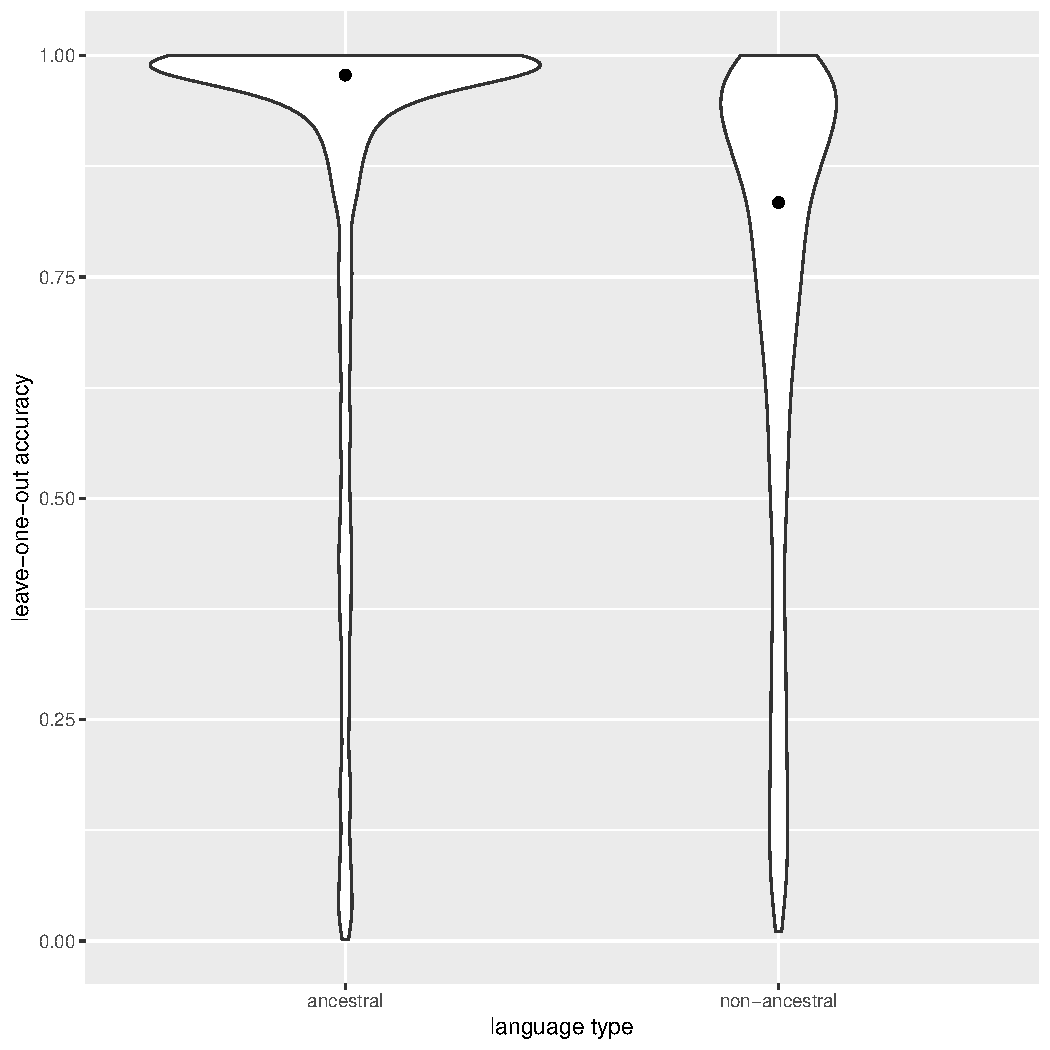
\includegraphics[width=.6\linewidth]{Figures-IE-grammar/LOO_accuracy.pdf}
    \caption{Held-out accuracy values for each language and feature, organized according to whether the feature is ancestral or not. Median values are indicated by dots.}
    \label{LOO}
\end{figure}

\section{Choice of prior probability at root}
\label{root.prior}

We investigate the extent to which our reconstructions are sensitive to choices of {\sc root prior}, a key ingredient in the {\sc pruning algorithm} \citep{Felsenstein1981,Felsenstein2004}. 
A standard practice in phylogenetics is to set the root prior to be equal to the stationary distribution of the variable of interest under the rates of the CTM process thought to characterize its evolution. For a binary character with a gain rate $\alpha$ and loss rate $\beta$, the stationary probability is equal to $\frac{\alpha}{\alpha + \beta}$.\footnote{An alternative parameterization for binary data is to draw a stationary probability $p \in [0,1]$ and a change rate $s$, from which gain and loss rates can be derived as $ps$ and $(1-p)s$, respectively.} 
For non-binary data, the stationary distribution $\boldsymbol{\pi}$ is a vector of probabilities satisfying the equations $\boldsymbol{\pi}Q$ and $\sum_{i=1}^{|\boldsymbol{\pi}|} \pi_i = 1$, where $Q$ is the CTM rate matrix. 
This practice presupposes that the character in question has been evolving for a `very long time according the particular model of [character evolution] we are using' (\citealt[255]{Felsenstein2004}; cf.\ \citealt{Cathcart2018modeling}). 

Though a sensible and established choice, this prior has the potential to influence the results of a phylogenetic reconstruction, particularly if the stationary probability is highly skewed toward a particular character value. 
To explore this issue, we carry out rate inference and reconstruction for the features in our data set using two alternative root priors, a {\sc uniform} prior which places equal prior probability of each value, and a {\sc dirichlet} prior which infers the distribution of values at the root as a free parameter to be inferred. For a variable with $D$ values, we set the prior probability of each value to $\frac{1}{D}$ under the uniform regime; under the Dirichlet regime, we place a $D$-length symmetric Dirichlet prior with a concentration parameter of $1$ over the feature distribution at the root.

The different prior regimes reconstruct the same features with highest probability for the majority of variables, but differ according to a fraction of variables. These are presented below, along with the probabilities with which they are reconstructed, for stationary probability (SP), uniform prior (UP) and Dirichlet prior (DP); cells for which an alternative regime agrees with the SP regime are blank.

\begin{center}
{\small
\begin{tabular}{p{.3\linewidth}p{.3\linewidth}p{.3\linewidth}}
\toprule
SP & UP & DP\\
\midrule
Clitic finite V: Category irrelevant (0.442) & Clitic finite V: V2 (0.270) & Clitic finite V: V2 (0.269)\\
\hline
Clitic Infinitive V: Category irrelevant (0.433) & Clitic Infinitive V: V2 (0.254) & Clitic Infinitive V: V2 (0.249)\\
\hline
Clitic Participle V: Category irrelevant (0.418) & Clitic Participle V: V2 (0.236) & Clitic Participle V: V2 (0.240)\\
\hline
No case on article (0.732) & Case on article (0.621) & Case on article (0.618)\\
\hline
No difference O and Dative (pronouns) (0.570) & Difference, O and Dative (pronouns) (0.519) & Difference, O and Dative (pronouns) (0.529)\\
\hline
No Future by participle (0.724) & Future by participle (0.767) & Future by participle (0.762)\\
\hline
Not more than 7 cases (0.583) & More than 7 cases (0.948) & More than 7 cases (0.950)\\
\hline
NRel: Noun - Relative (0.627) & NRel: Relative - Noun (0.315) & NRel: Relative - Noun (0.316)\\
\hline
Possessor - Noun (0.585) & Possessor - Noun and Noun - Possessor (0.374) & Possessor - Noun and Noun - Possessor (0.377)\\
\hline
Reflexive with Agent (0.959) & Reflexive not with Agent (0.505) & Reflexive not with Agent (0.505)\\
\hline
Simple past: Full A Agreement (0.386) & \centering --- & Simple past: Syncretic A Agreement (0.206)\\
\bottomrule
\end{tabular}
}
\end{center}

It is worth noting that with a handful of exceptions, the features reconstructed differently by the alternative models are reconstructed with high uncertainty, and as a whole, the differing features are not of key importance to the canonical model of reconstruction supported by the main results presented in this paper (see \S3, {\sc Results: reconstruction}).


\section{Entry/Gain and Exit/Loss Rates}

For each multistate character, we compute the mean rate at which each state is gained or lost in the following manner. We compute the gain rate for state $i$, or rate at which state $i$ is entered, as follows, where $R(j \rightarrow i)$ denotes the rate from state \emph{j} to state \emph{i}, and $p(s)$ denotes the equilibrium or stationary probability of state $s$:
$$
\frac{\sum_{j \neq i} p(j) R(j \rightarrow i)}{\sum_{j \neq i} p(j)}
$$
The loss rate for state $i$, or rate at which state $i$ is exited, is computed as follows:
$$
\sum_{j \neq i} R(i \rightarrow j)
$$

We thank Gerhard J\"ager for deriving the equation for entry rates for us, and for providing the following proof, which we reproduce with his permission:

\begin{proof}
Let us first consider the simpler case where we have a stochastic transition matrix $P$. We are interested in the probability of switching from state $a$ or $b$ to state $c$ or $d$:
$$
P(\{c,d\}|\{a,b\})
$$
According to the definition of conditional probability, this is:
$$
\frac{P(\{a,b\} \rightarrow \{c,d\})}{P(\{a,b\})}
$$
This is only defined if we know $P(\{a,b\})$, so we assume that the process is in equilibrium and that these are the equilibrium probabilities. Since $a$ and $b$ are disjoint, we have $P(\{a,b\}) = P_E(a) + P_E(b)$ ($P_E$ being the equilibrium probability.)

There are four different possible transitions in the numerator, which are mutually disjoint, so we have 

$$
\frac{P(a \rightarrow b) + P(a \rightarrow d) + P(b \rightarrow c) + P(b \rightarrow d)}{P_E(a)+P_E(b)}
$$

Again, $P(a \rightarrow c)$ is only defined if we know the probability of the process starting in $a$. Under the equilibrium assumption, we have $P(a \rightarrow c) = P_E(a)P(c|a)$, and likewise for the other transitions.

Putting this together, we have

\begin{align*}
P(\{c,d\}|\{a,b\}) & = \frac{P_E(a)P(c|a) + P_E(a)P(d|a) + P_E(b)P(c|b) + P_E(b)P(d|b)}{P_E(a) + P_E(b)}\\
 & = \frac{P_E(a)(P(c|a) + P(d|a)) + P_E(b)(P(c|b) + P(d|b))}{P_E(a) + P_E(b)}\\
\end{align*}

Now let us assume that we have a continuous-time Markov process, where $P$ is time dependent. 
The {\em rate} $r_{\{a,b\} \rightarrow \{c,d\}}$ is the limit of the expected number of transitions from 
$\{a,b\}$ 
into 
$\{c,d\}$ 
per 
time period for infinitesimal time periods, provided the system starts in $\{a,b\}$:

\begin{align*}
    r_{\{a,b\} \rightarrow \{c,d\}} & = \frac{d}{dt} P_t(\{c,d\}|\{a,b\})\Bigr|_{t=0}\\
     & = \frac{d}{dt}\frac{P_E(a)(P(c|a) + P(d|a)) + P_E(b)(P(c|b) + P(d|b))}{P_E(a) + P_E(b)}\Bigr|_{t=0}
\end{align*}
$P_E$ does not depend on $t$, and $\frac{d}{dt}P_t(c|a)\Bigr|_{t=0} = r_{ac}$ (and likewise for other transitions); therefore we get
$$
r_{\{a,b\} \rightarrow \{c,d\}} = \frac{P_E(a)(r_{ac} + r_{ad}) + P_E(b)(r_{bc} + r_{bd})}{P_E(a) + P_E(b)}
$$

\end{proof}

\bibliographystyle{chicagoa}
\bibliography{Reconstructing_evolution}


\end{appendices}

\pagebreak

\pagestyle{empty}


\section*{Supplementary materials: data and results}

\subsection*{S1}
Languages, including latitude and longitude, used in the current study.

\begin{longtable}{lll}
\toprule
Language & Longitude & Latitude\\
\midrule
Albanian (Tosk) & 19.988251 & 40.446947\\
Angloromani & -2.355272 & 53.779521\\
Ashkun & 70.791057 & 35.255909\\
Assamese & 91.79022 & 26.143538\\
Avestan & 55.9499 & 31.70708\\
Baluchi & 65.03622 & 26.27794\\
Bengali & 88.36119 & 22.566866\\
Breton & -4.102864 & 47.995619\\
Bulgarian & 23.3535 & 42.698586\\
Catalan & 2.179642 & 41.379225\\
Classical Greek & 23.999205 & 37.696861\\
Cornish & -5.567517 & 50.191816\\
Croatian & 15.992661 & 45.813486\\
Czech & 14.468136 & 50.071244\\
Danish & 12.583182 & 55.679885\\
Dutch & 4.898126 & 52.374367\\
Elfdalian & 14.040485 & 61.225938\\
English & -0.100059 & 51.497728\\
Faroese & -6.773322 & 62.009754\\
French & 2.347857 & 48.854451\\
Frisian & 5.795597 & 53.20394\\
Friulian & 13.485001 & 46.127028\\
German & 13.409092 & 52.520822\\
Gilaki & 49.283999 & 37.526056\\
Gothic & 20.199324 & 53.042874\\
Gujarati & 72.139869 & 22.44456\\
Hindi & 77.224996 & 28.625252\\
Hittite & 34.621158 & 40.013951\\
Icelandic & -21.939672 & 64.144237\\
Irish & -9.301101 & 53.244432\\
Italian & 12.385145 & 43.115956\\
Kashmiri & 75.939182 & 34.322996\\
Kati & 71.314571 & 35.799992\\
Khowar & 72.51658 & 36.457958\\
Konkani & 72.871066 & 19.262081\\
Kurdish (Kurmanji) & 43.822746 & 37.788081\\
Kurdish (Sorani) & 45.728512 & 35.821161\\
Ladin & 11.923755 & 46.657384\\
Latin & 12.4923 & 41.890189\\
Latvian & 24.113274 & 56.915\\
Lithuanian & 25.255852 & 54.680183\\
Low German & 9.488653 & 53.931994\\
Luwian & 36.788273 & 36.620598\\
Maithili & 86.155454 & 26.075397\\
Maldivian & 73.511939 & 4.17191\\
Manx & -4.484657 & 54.151988\\
Marathi & 75.494714 & 19.38701\\
Middle Breton & -1.532472 & 47.207854\\
Middle Dutch & 5.959192 & 52.213073\\
Middle English & -0.758622 & 51.313607\\
Middle Greek & 28.997555 & 41.058644\\
Middle High German & 9.717403 & 48.742717\\
Middle Irish & -8.634407 & 52.658918\\
Middle Low German & 10.68504 & 53.867783\\
Middle Persian & 51.675883 & 32.647027\\
Middle Welsh & -3.380017 & 52.240359\\
Modern Armenian & 44.527159 & 40.147389\\
Modern Greek & 23.694334 & 38.028622\\
Nepali & 89.243625 & 26.659702\\
Norwegian (Bokm\r{a}l) & 10.740802 & 59.912785\\
Norwegian (Nynorsk) & 5.075361 & 60.330984\\
Old Church Slavonic & 30.453243 & 50.415519\\
Old Dutch & 5.123259 & 52.09095\\
Old English & -1.314163 & 51.060696\\
Old French & 2.347857 & 48.854451\\
Old Frisian & 6.567738 & 53.215696\\
Old High German & 9.962616 & 49.795477\\
Old Irish & -6.873827 & 53.726794\\
Old Italian & 11.249249 & 43.776281\\
Old Norse & 10.397522 & 63.426975\\
Old Persian & 52.891196 & 29.935501\\
Old Portuguese & -8.629141 & 41.15818\\
Old Proven\c{c}al & 6.222519 & 43.426825\\
Old Prussian & 19.900799 & 54.436292\\
Old Russian & 31.275345 & 58.521428\\
Old Saxon & 8.806043 & 53.07585\\
Old Spanish & -4.023666 & 39.857094\\
Old Swedish & 16.321936 & 58.481083\\
Oriya & 86.278412 & 20.608549\\
Ossetian (Iron) & 44.675689 & 43.043802\\
Pali & 83.000379 & 27.617895\\
Parachi & 69.702595 & 34.832889\\
Pashto & 68.188804 & 31.432929\\
Persian & 55.748043 & 32.735314\\
Polish & 20.994015 & 52.237892\\
Portuguese & -9.135132 & 38.708043\\
Prakrit & 84.727979 & 25.379098\\
Prasun & 70.741619 & 35.33661\\
Proven\c{c}al & 6.222519 & 43.426825\\
Punjabi & 74.349411 & 31.536604\\
Romani (Arli) & 19.881168 & 42.970349\\
Romani (Bugurd\v{z}i) & 21.222651 & 42.118106\\
Romani (Burgenland) & 16.377534 & 47.193164\\
Romani (Kale) & 21.470967 & 60.972087\\
Romani (Kelderash) & 22.495093 & 47.187683\\
Romani (Lovara) & 23.090199 & 47.401544\\
Romani (Sepe\v{c}ides) & 27.131666 & 38.392804\\
Romani (Sinte) & 10.203424 & 51.4992\\
Romanian & 26.086373 & 44.427511\\
Romansh & 9.838341 & 46.496755\\
Russian & 37.64843 & 55.677584\\
Sanskrit & 76.28612 & 23.511415\\
Sardinian & 9.32737 & 40.31746\\
Scandoromani & 13.158622 & 59.481307\\
Scottish Gaelic & -7.368974 & 57.16276\\
Serbian & 20.472164 & 44.801327\\
Shughni & 71.503041 & 38.389635\\
Sicilian & 13.368345 & 38.115141\\
Sindhi & 69.674802 & 23.253479\\
Sinhalese & 79.85635 & 6.935115\\
Slovene & 14.50823 & 46.050593\\
Sogdian & 66.962682 & 39.646576\\
Spanish & -3.703482 & 40.416881\\
Swedish & 17.438718 & 59.73823\\
Swiss German & 8.538354 & 47.36888\\
Tajik & 70.342617 & 38.663458\\
Talysh & 48.730017 & 38.854174\\
Tocharian A & 86.154785 & 41.760336\\
Tocharian B & 81.514435 & 41.645502=\\
Ukrainian & 30.525414 & 50.449474\\
Upper Sorbian & 14.425442 & 51.179914\\
Urdu & 73.018423 & 33.681135\\
Wakhi & 72.760057 & 37.219477\\
Walloon & 4.865382 & 50.464478\\
Welsh & -4.38518 & 52.926407\\
Yiddish & 24.031167 & 49.853028\\
\bottomrule
\end{longtable}

\pagebreak

\subsection*{S2a}

List of typological features (from DiACL database https://diacl.ht.lu.se) used in the current study.

Grid = topmost organizational unit in database, corresponding to linguistic domain; Feature = second organizational unit in database; Feature description = Description of Feature in database; Variant = lowest organizational unit in database; Variant description = description of variant in database; ID = unique database ID of Variant.

{\footnotesize 
\begin{longtable}{p{.12\linewidth}p{.12\linewidth}p{.16\linewidth}p{.12\linewidth}p{.26\linewidth}p{.6\linewidth}}
Grid & Feature & Feature description & Variant & Variant description &  ID\\
Word order & Adpositions & Do adpositions normally occur before or after the noun? & Prep & Does the language have a substantial set of prepositions? E.g. English in the house & 213\\
Word order & Adpositions & Do adpositions normally occur before or after the noun? & Post & Does the language have a substantial set of postpositions? & 214\\
Word order & Noun-adjective & Do adjectives normally occur before or after the noun? & NA & Do most adjectives occur after the noun? & 215\\
Word order & Noun-adjective & Do adjectives normally occur before or after the noun? & AN & Do most adjectives occur before the noun? & 216\\
Word order & Noun-relative clause & Do relative clauses normally occur before or after the noun? & NRel & Do most relative clauses occur after the noun? & 217\\
Word order & Noun-relative clause & Do relative clauses normally occur before or after the noun? & RelN & Do most relative clauses occur before the noun? & 218\\
Word order & Noun-possessor & Do possessors normally occur before or after the noun? & N-Poss & Do most possessors occur after the noun they possess? The possessor should be an animate noun, and neither a proper name nor a pronoun! & 219\\
Word order & Noun-possessor & Do possessors normally occur before or after the noun? & Poss-N & Do most possessors occur before the noun they possess? The possessor should be an animate noun, and neither a proper name nor a pronoun! & 220\\
Word order & WH-element & What is the position of the WH-question word?  & WH-initial & Is the WH-question word always obligatorily the first element in a question (e.g., it does not trigger inversion)? & 221\\
Word order & WH-element & What is the position of the WH-question word?  & WH-V & Does the WH-question word always immediately precede the verb (i.e., stand directly before the verb, either initially or non-initially)? & 222\\
Word order & Main clause & What is the canonical (neutral) word order in a main clause? & SVO & What is the canonical (neutral) word order in a main clause? NB: V2 languages like Swe and Ger do NOT count as SVO even though SVO is most frequent. & 223\\
Word order & Main clause & What is the canonical (neutral) word order in a main clause? & V2 & V2 implies that initial adverb triggers V-SUBJ word order (Swedish, German etc.). & 224\\
Word order & Main clause & What is the canonical (neutral) word order in a main clause? & VSO & What is the canonical (neutral) word order in a main clause? & 225\\
Word order & Main clause & What is the canonical (neutral) word order in a main clause? & SOV & What is the canonical (neutral) word order in a main clause? & 226\\
Word order & Subordinate clause & What is the canonical (neutral) word order in a subordinate clause?  & SVO & What is the canonical (neutral) word order in a subordinate clause? NB: V2 languages like Swe and Ger do NOT count as SVO even though SVO is most frequent. & 227\\
Word order & Subordinate clause & What is the canonical (neutral) word order in a subordinate clause?  & V2 & V2 implies that initial adverb triggers V-SUBJ word order (Swedish, German etc.). & 228\\
Word order & Subordinate clause & What is the canonical (neutral) word order in a subordinate clause?  & VSO & What is the canonical (neutral) word order in a subordinate clause?  & 229\\
Word order & Subordinate clause & What is the canonical (neutral) word order in a subordinate clause?  & SOV & What is the canonical (neutral) word order in a subordinate clause?  & 230\\
Word order & Infinitive & Does the object normally occur before or after an infinitive? E.g.: to make pancakes (VO) Pfannkuchen machen (OV) & VO &  & 231\\
Word order & Infinitive & Does the object normally occur before or after an infinitive? E.g.: to make pancakes (VO) Pfannkuchen machen (OV) & OV &  & 232\\
Word order & Participle & Does the object normally occur before or after a participle?  E.g.: making pancakes (VO)  Pfannkuchen machend (OV) & VO &  & 233\\
Word order & Participle & Does the object normally occur before or after a participle?  E.g.: making pancakes (VO)  Pfannkuchen machend (OV) & OV &  & 234\\
Word order & Clitic pronouns finite verb & Does the clitic object pronoun normally occur before or after a finite verb?  E.g.: Je les fais. (OV)  If a language does not have clitic object pronouns, it would be 0 in both OV and VO. & VO &  & 235\\
Word order & Clitic pronouns finite verb & Does the clitic object pronoun normally occur before or after a finite verb?  E.g.: Je les fais. (OV)  If a language does not have clitic object pronouns, it would be 0 in both OV and VO. & OV &  & 236\\
Word order & Clitic pronouns finite verb & Does the clitic object pronoun normally occur before or after a finite verb?  E.g.: Je les fais. (OV)  If a language does not have clitic object pronouns, it would be 0 in both OV and VO. & 2nd position & Does the clitic pronoun always occur in 2nd position, not specifically before or after the verb? (Wackernagel position) & 237\\
Word order & Clitic pronouns infinitive & Does the clitic object pronoun normally occur before or after an infinitive? E.g.: Je veux les faire. (OV) If a language does not have clitic object pronouns, it would be 0 in both OV and VO. & VO &  & 238\\
Word order & Clitic pronouns infinitive & Does the clitic object pronoun normally occur before or after an infinitive? E.g.: Je veux les faire. (OV) If a language does not have clitic object pronouns, it would be 0 in both OV and VO. & OV &  & 239\\
Word order & Clitic pronouns infinitive & Does the clitic object pronoun normally occur before or after an infinitive? E.g.: Je veux les faire. (OV) If a language does not have clitic object pronouns, it would be 0 in both OV and VO. & 2nd position & Does the clitic pronoun always occur in 2nd position, not specifically before or after the verb? & 240\\
Word order & Clitic pronouns participle & Does the clitic object pronoun normally occur before or after a participle? E.g.: En les faisant... (OV) If a language does not have clitic object pronouns, it would be 0 in both OV and VO. & VO &  & 241\\
Word order & Clitic pronouns participle & Does the clitic object pronoun normally occur before or after a participle? E.g.: En les faisant... (OV) If a language does not have clitic object pronouns, it would be 0 in both OV and VO. & OV &  & 242\\
Word order & Clitic pronouns participle & Does the clitic object pronoun normally occur before or after a participle? E.g.: En les faisant... (OV) If a language does not have clitic object pronouns, it would be 0 in both OV and VO. & 2nd position & Does the clitic pronoun always occur in 2nd position, not specifically before or after the verb? & 243\\
Nominal morphology & Nominal case & What is the realization of case at nouns (nominal heads)? & O-case & Are there different noun forms for agent and object case? (English: 0 (no cases)  Russian: 1 (different noun forms for accusative and nominative)  Basque: 1 (different noun forms for ergative and absolutive) & 244\\
Nominal morphology & Nominal case & What is the realization of case at nouns (nominal heads)? & DAT & Is there a specific case form for the recipient, which is different from the case form of, e.g., the object?  (E.g. The man gives a book (O) to the child (DAT)) & 245\\
Nominal morphology & Nominal case & What is the realization of case at nouns (nominal heads)? & GEN & Is there a special case form to express genitive, which is different from the agent/object case? & 246\\
Nominal morphology & Nominal case & What is the realization of case at nouns (nominal heads)? & GEN/DAT & Is there a special noun form to express genitive, which is not the same as dative (recipient) case? & 247\\
Nominal morphology & Nominal case & What is the realization of case at nouns (nominal heads)? & VOC & Is there a special noun form to express vocative which is not the same as agent or object case? & 248\\
Nominal morphology & Nominal case & What is the realization of case at nouns (nominal heads)? & OBL-Cases & Are there any cases besides agent, object, genitive, dative, and vocative? (E.g., local cases) & 249\\
Nominal morphology & Nominal case & What is the realization of case at nouns (nominal heads)? & $>$7 Cases & Are there more than 7 cases? & 250\\
Nominal morphology & Nominal case & What is the realization of case at nouns (nominal heads)? & AGGL.CASE & Are there cases which are visibly agglutinative, i.e., built up by several distinct, segmentable affixes? & 251\\
Nominal morphology & Nominal case & What is the realization of case at nouns (nominal heads)? & AGGL.CASE.NR & Are plural cases formed by combining an (infixed) plural affix and a case affix in an agglutinative manner? & 252\\
Nominal morphology & Pronominal case & What is the realization of case at pronouns (pronominal heads)? Mainly 1st and 2nd person pronouns, ignoring 3rd person pronouns (which often come from demonstratives). & A $\neq$�O & In pronouns, is the marking different for the case of the agent and object?  & 253\\
Nominal morphology & Pronominal case & What is the realization of case at pronouns (pronominal heads)? Mainly 1st and 2nd person pronouns, ignoring 3rd person pronouns (which often come from demonstratives). & DAT $\neq$�O & In pronouns, is the marking different for the case of the recipient and the object?  & 254\\
Nominal morphology & Pronominal case & What is the realization of case at pronouns (pronominal heads)? Mainly 1st and 2nd person pronouns, ignoring 3rd person pronouns (which often come from demonstratives). & VOC & See Nominal case & 255\\
Nominal morphology & Pronominal case & What is the realization of case at pronouns (pronominal heads)? Mainly 1st and 2nd person pronouns, ignoring 3rd person pronouns (which often come from demonstratives). & OBL-Cases & See Nominal case & 256\\
Nominal morphology & Pronominal case & What is the realization of case at pronouns (pronominal heads)? Mainly 1st and 2nd person pronouns, ignoring 3rd person pronouns (which often come from demonstratives). & $>$7 Cases & See Nominal case & 257\\
Nominal morphology & Pronominal case & What is the realization of case at pronouns (pronominal heads)? Mainly 1st and 2nd person pronouns, ignoring 3rd person pronouns (which often come from demonstratives). & AGGL.CASE & See Nominal case & 258\\
Nominal morphology & Pronominal case & What is the realization of case at pronouns (pronominal heads)? Mainly 1st and 2nd person pronouns, ignoring 3rd person pronouns (which often come from demonstratives). & AGGL.CASE.NR & See Nominal case & 259\\
Nominal morphology & Case marking & On which elements of the NP is the case marking obligatory? & CASE-LAST & Is the case marking obligatory on the last element of the NP (i.e., it is only realized once in the NP, even if it consists of several elements)? & 260\\
Nominal morphology & Case marking & On which elements of the NP is the case marking obligatory? & CASE-FIRST & Is the case marking obligatory on the first element of the NP (i.e., it is only realized once in the NP, even if it consists of several elements)? & 261\\
Nominal morphology & Case marking & On which elements of the NP is the case marking obligatory? & CASE-N & Is the case marking obligatory realized on the noun? & 262\\
Nominal morphology & Case marking & On which elements of the NP is the case marking obligatory? & CASE-ADJ & Is the case marking obligatory on the adjective? & 263\\
Nominal morphology & Case marking & On which elements of the NP is the case marking obligatory? & CASE-ART & Is the case marking realized on the article? & 264\\
Nominal morphology & Gender / noun class & How is gender / noun class realized in the language? & M/F & Is there an obligatory gender distinction between masculine and feminine realized on an agreeing article or adjective?  Can be either on the adjective (Russian) or on both the article and the adjective (German), or even on a verb (as in some NE Caucasian languages).  & 265\\
Nominal morphology & Gender / noun class & How is gender / noun class realized in the language? & NEUTR & Is there a special neutral gender for nouns realized on an agreeing article,  adjective or verb? & 266\\
Nominal morphology & Gender / noun class & How is gender / noun class realized in the language? & ANIM & Is there a special noun class for non-human animates realized on an agreeing article, adjective or verb? & 267\\
Nominal morphology & Gender / noun class & How is gender / noun class realized in the language? & $<$5 GENDER & Are there more than 5 noun classes (or genders)? & 268\\
Nominal morphology & Definiteness marking & How is definiteness marking realized in the language? & DEF-ART & Is there a special word class of definite articles which occur in NPs without adjectives?  (E.g.: German, English but not Swedish) & 269\\
Nominal morphology & Definiteness marking & How is definiteness marking realized in the language? & N-DEF & Is there a suffix for definiteness on the noun? (E.g.: Swedish but not English!) & 270\\
Nominal morphology & Definiteness marking & How is definiteness marking realized in the language? & ADJ-DEF & Is there a suffix for definiteness on the adjective? This includes cases when the ADJ has a different form in definite and indefinite NPs (Swe ``det stora huset", Ger ``das grosse Haus"). & 271\\
Nominal morphology & Definiteness marking & How is definiteness marking realized in the language? & DEF-LAST & Is the definiteness marking obligatory on the last element of the NP (so it is only realized once in the NP, even if it consists of several elements)?  If there is no definiteness marking at all, it will be 0! & 272\\
Nominal morphology & Definiteness marking & How is definiteness marking realized in the language? & DEF-FIRST & Is the definiteness marking obligatory on the first element of the NP (so it is only realized once in the NP, even if it consists of several elements)?  If there is no definiteness marking at all, it will be 0! & 273\\
Nominal morphology & Gender agreement & How is gender agreement realized in the language? & PRED-ADJ & Does a predicative adjective agree with the subject of the clause in gender? & 274\\
Nominal morphology & Preposition agreement & How is preposition agreement realized in the language? & PREP-PRON-AGR & Can a preposition agree in person with its object? & 275\\
Verbal morphology & Simple PAST, A & In simple past, how is verbal agreement realized with respect to the agent? & PST:A-AGR-FULL & In simple past: does the verb crossreference the agent in all persons /numbers? & 276\\
Verbal morphology & Simple PAST, A & In simple past, how is verbal agreement realized with respect to the agent? & PST:NO-A-AGR & In simple past: does the verb not crossreference the agent on the verb at all (e.g., Swedish)? & 277\\
Verbal morphology & Simple PAST, A & In simple past, how is verbal agreement realized with respect to the agent? & PST:A-Gender-AGR & In simple past, does the verb agree in gender with the subject of a transitive verb? (e.g., Russian, Polish). & 278\\
Verbal morphology & Simple PAST, O & In simple past, how is verbal agreement realized with respect to the object?  & PST:O-AGR-FULL & In simple past: does the verb crossreference the object in all persons /numbers? & 279\\
Verbal morphology & Simple PAST, O & In simple past, how is verbal agreement realized with respect to the object?  & PST:NO-O-AGR & In simple past: does the verb not crossreference the object on the verb at all (e.g., Swedish, English, Russian)? & 280\\
Verbal morphology & Simple PAST, O & In simple past, how is verbal agreement realized with respect to the object?  & PST:O-Gender-AGR & In simple past, does the verb agree in gender with the object? & 281\\
Verbal morphology & Simple PAST, DAT & In simple past, how is verbal agreement realized with respect to the indirect object of ditransitive verbs? & PST:DAT-AGR-FULL & In simple past: does the verb crossreference the dative in all persons /numbers? & 282\\
Verbal morphology & Simple PAST, DAT & In simple past, how is verbal agreement realized with respect to the indirect object of ditransitive verbs? & PST:NO-DAT-AGR & In simple past: does the verb not crossreference the dative on the verb at all (e.g., Swedish, English, Russian) & 283\\
Verbal morphology & Simple PAST, DAT & In simple past, how is verbal agreement realized with respect to the indirect object of ditransitive verbs? & PST:DAT-Gender-AGR & In simple past, does the verb agree in gender with the indirect object of a ditransitive verb? & 284\\
Verbal morphology & Present progressive, A & In present progressive: how is verbal agreement realized with respect to the agent?  & PROG:A-AGR-FULL & In present progressive: does the verb crossreference the agent in all persons /numbers? & 285\\
Verbal morphology & Present progressive, A & In present progressive: how is verbal agreement realized with respect to the agent?  & PROG:NO-A-AGR & In present progressive: does the verb not crossreference the agent on the verb at all (e.g., Swedish) & 286\\
Verbal morphology & Present progressive, A & In present progressive: how is verbal agreement realized with respect to the agent?  & PROG:A-Gender-AGR & In present progressive, does the verb agree in gender with the subject of a transitive verb? & 287\\
Verbal morphology & Present progressive, O & In present progressive, how is verbal agreement organized with respect to the object? & PROG:O-AGR-FULL & In present progressive: does the verb crossreference the object in all persons /numbers? & 288\\
Verbal morphology & Present progressive, O & In present progressive, how is verbal agreement organized with respect to the object? & PROG:NO-O-AGR & In present progressive: does the verb not crossreference the object on the verb at all (e.g. Swedish, Russian)? & 289\\
Verbal morphology & Present progressive, O & In present progressive, how is verbal agreement organized with respect to the object? & PROG:O-Gender-AGR & In present progressive, does the verb agree in gender with the object of a transitive verb? & 290\\
Verbal morphology & Present progressive, DAT & In present progressive, how is verbal agreement organized with respect to the indirect object of ditransitive verbs? & PROG:DAT-AGR-FULL & Iin present progressive: does the verb crossreference the indirect object of a ditransitive verb in all persons /numbers? & 291\\
Verbal morphology & Present progressive, DAT & In present progressive, how is verbal agreement organized with respect to the indirect object of ditransitive verbs? & PROG:NO-DAT-AGR & In present progressive: does the verb not crossreference the indirect object of ditransitive verbs at all (e.g. Swedish, English, Russian)? & 292\\
Verbal morphology & Present progressive, DAT & In present progressive, how is verbal agreement organized with respect to the indirect object of ditransitive verbs? & PROG:DAT-Gender-AGR & In the present progressive, does the verb agree in gender with the indirect object of a ditransitive verb? & 293\\
Verbal morphology & Allocutive agreement & Does the verb agree with the receiver (the person one is speaking to) without the speaker being an argument in the sentence (allocutive agreement, probably no for all languages but Basque!)  & ALLOC & Does the verb agree with the receiver (the person one is speaking to) without the speaker being an argument in the sentence (allocutive agreement, probably no for all languages but Basque!) & 294\\
Tense & Future & How is future realized in the language? & FUT.AUX & Is there a future formed by an auxiliary? (E.g., will in English? & 295\\
Tense & Future & How is future realized in the language? & PERF.FUT & Is there a future formed by using the perfective aspect? (0 if the language does not have verbal aspects! E.g., Russian, Georgian) & 296\\
Tense & Future & How is future realized in the language? & FUT.Participle & Is there a future formed by a participle? (E.g., Armenian, Basque) & 297\\
Tense & Future & How is future realized in the language? & FUT.Particle & Is there a future formed by a particle preceding a finite verb? (E.g., Albanian) & 298\\
Tense & Future & How is future realized in the language? & FUT.Synth & Is there a synthetical future? (E.g., French, Spanish) & 299\\
Tense & Continous present & How is present progressive realized in the language? & Present & Is there a synthetic present in progressive function? & 300\\
Tense & Continous present & How is present progressive realized in the language? & Progressive present & Is there a progressive present form constructed by combining a present participle with a finite auxiliary verb? & 301\\
Alignment & Noun: Simple Past & In simple past: how is the marking of subject and object of nouns realized? & N:PST:A=O? & In simple past: Is the noun form for A the same as for O? Ie: Does the noun look the same when it is subject of a transitive clause than when it is object of a transitive clause? & 302\\
Alignment & Noun: Simple Past & In simple past: how is the marking of subject and object of nouns realized? & N:PST:A=Sa? & In simple past:Is the noun form for A the same as for Sa? Ie: Does the noun look the same when it is subject of a transitive clause as when it is subject of an agentive intransitive verb such as ``work" or ``dance"? & 303\\
Alignment & Noun: Simple Past & In simple past: how is the marking of subject and object of nouns realized? & N:PST: O=So? & In simple past: Is the noun form for O the same as for So? Ie: Does the noun look the same when it is object of a transitive clause as when it is subject of an unaccusative verb such as ``fall" or ``die"? & 304\\
Alignment & Noun: Simple Past & In simple past: how is the marking of subject and object of nouns realized? & N:PST: Sa=So? & In simple past: Does a noun bear the same case form when it is Sa (subject of e.g. work) or So (subject of e.g. fall or die)? Ie: There does not exist a split into stative and active intransitive verbs. & 305\\
Alignment & Noun: Present Progressive & In present progressive: how is the marking of subject and object of nouns realized?  & N:PROG: A=O? & In present progressive: Is the noun form for A the same as for O?  I.e.: Does the noun look the same when it is subject of a transitive clause and when it is object of a transitive clause? & 306\\
Alignment & Noun: Present Progressive & In present progressive: how is the marking of subject and object of nouns realized?  & N:PROG: A=Sa? & In present progressive:Is the noun form for A the same as for Sa?  I.e.: Does the noun look the same when it is subject of a transitive clause and when it is subject of an agentive intransitive verb such as ``work" or ``dance"? & 307\\
Alignment & Noun: Present Progressive & In present progressive: how is the marking of subject and object of nouns realized?  & N:PROG: O=So? & In present progressive: Is the noun form for O the same as for So?  I.e.: Does the noun look the same when it is object of a transitive clause and when it is subject of an unaccusative verb such as ``fall" or ``die"? & 308\\
Alignment & Noun: Present Progressive & In present progressive: how is the marking of subject and object of nouns realized?  & N:PROG: Sa=So? & In present progressive: does a noun bear the same case form when it is Sa (subject of e.g., ``work") or So (subject of e.g., ``fall" or ``die")?  I.e.: The language does not have a split between stative and active intransitive verbs. & 309\\
Alignment & Pronoun: Simple Past & In present progressive: how is the marking of subject and object of pronouns realized? & P:PST: A=O? & In simple past: Is the pronoun form for A the same as for O?  I.e.: Does the pronoun look the same when it is subject of a transitive clause than when it is object of a transitive clause? & 310\\
Alignment & Pronoun: Simple Past & In present progressive: how is the marking of subject and object of pronouns realized? & P:PST: A=Sa? & In simple past: Is the pronoun form for A the same as for Sa?  I.e.: Does the pronoun look the same when it is subject of a transitive clause than when it is subject of an agentive intransitive verb such as ``work" or ``dance"? & 311\\
Alignment & Pronoun: Simple Past & In present progressive: how is the marking of subject and object of pronouns realized? & P:PST: O=So? & In simple past: Is the pronoun form for O the same as for So?  I.e.: Does the pronoun look the same when it is object of a transitive clause than when it is subject of an unaccusative verb such as ``fall" or ``die"? & 312\\
Alignment & Pronoun: Simple Past & In present progressive: how is the marking of subject and object of pronouns realized? & P:PST: Sa=So? & In simple past: Does the pronoun bear the same case form when it is Sa (subject of e.g. work) or So (subject of e.g. fall or die)?  I.e.: There does not exist a split into stative and active intransitive verbs. & 313\\
Alignment & Pronoun: Present Progressive &  In present progressive: how is the marking of subject and object of pronouns realized? & P:PROG: A=O? & In present progressive: Is the pronoun form for A the same as for O?  I.e.: Does the pronoun look the same when it is subject of a transitive clause than when it is object of a transitive clause? & 314\\
Alignment & Pronoun: Present Progressive &  In present progressive: how is the marking of subject and object of pronouns realized? & P:PROG: A=Sa? & In present progressive:Is the pronoun form for A the same as for Sa?  I.e.: Does the pronoun look the same when it is subject of a transitive clause as when it is subject of an agentive intransitive verb such as ``work" or ``dance"? & 315\\
Alignment & Pronoun: Present Progressive &  In present progressive: how is the marking of subject and object of pronouns realized? & P:PROG: O=So? & In present progressive: Is the pronoun form for O the same as for So?  I.e.: Does the pronoun look the same when it is object of a transitive clause than when it is subject of an unaccusative verb such as ``die" or ``fall"? & 316\\
Alignment & Pronoun: Present Progressive &  In present progressive: how is the marking of subject and object of pronouns realized? & P:PROG: Sa=So? & In present progressive: Does a pronoun bear the same case form when it is Sa (subject of e.g. work) or So (subject of e.g. fall or die)? Ie: There does not exist a split into stative and active intransitive verbs. & 317\\
Alignment & Verb: Simple Past & In simple past, how is alignment realized on the verb? & V:PST:A=O? & In simple past: Is the verb affix for A the same as for O?  I.e.: Does the verb look the same when it refers to the  subject of a transitive clause than when it refers to the object of a transitive clause?  If there is no O-marking on the verb, but there is an S-marking, the answer would be no, they do not look the same. (e.g., German, Russian)  If there is neither an O, nor an A marking, like in Swedish, the answer would be yes, they look the same! & 318\\
Alignment & Verb: Simple Past & In simple past, how is alignment realized on the verb? & V:PST:A=Sa? & In simple past: Is the verb affix for A the same as for Sa?  I.e.: Does the verb look the same when it refers to subject of a transitive clause than when it refers to subject of an agentive intransitive verb like ``work" or ``dance"? & 319\\
Alignment & Verb: Simple Past & In simple past, how is alignment realized on the verb? & V:PST:O=So? & In simple past: Is the verb affix for O the same as for So?  I.e.: Does the verb look the same when it refers to the object of a transitive clause as when it refers to the subject of an unaccusative verb (such as ``fall" or ``die")? & 320\\
Alignment & Verb: Simple Past & In simple past, how is alignment realized on the verb? & V:PST:Sa=So? & In simple past: Is the verb affix the same for Sa (subject of e.g. work) as or So (subject of e.g. fall or die)? I.e., does the verb agreement affix look the same regardless of whether the verb is ``work" or ``die" (as in German: ``arbeitete-st", ``starb-st").  I.e.: There does not exist a split into unaccusative and agentive intransitive verbs. & 321\\
Alignment & Verb: Present Progressive & In present progressive, how is alignment realized on the verb? & V:PROG: A=O? & In present progressive: Is the verb affix for A the same as for O? Ie: Does the verb look the same when it refers to the  subject of a transitive clause than when it refers to the object of a transitive clause? If there is no O-marking on the verb, but there is an S-marking, the answer would be no, they do not look the same. (e.g. German, Russian) If there is neither an O, nor an A marking like in Swedish, the answer would be yes, they look the same! & 322\\
Alignment & Verb: Present Progressive & In present progressive, how is alignment realized on the verb? & V:PROG: A=Sa? & In present progressive:Is the verb affix for A the same as for Sa? Ie: Does the verb look the same when it refers to subject of a transitive clause as when it refers to subject of an agentive intransitive verb such as ``work"? & 323\\
Alignment & Verb: Present Progressive & In present progressive, how is alignment realized on the verb? & V:PROG: O=So? & In present progressive: Is the verb affix the same for O as for So? Ie: Does the verb look the same when it refers to the object of a transitive clause as when it refers to the subject of an unaccusative verb (such as ``fall" or ``die")? & 324\\
Alignment & Verb: Present Progressive & In present progressive, how is alignment realized on the verb? & V:PROG: Sa=So? & In present progressive: Is the verb affix the same for Sa (subject of e.g. ``work") as or So (subject of e.g. ``fall" or ``die")? I.e. does the verb agreement affix look the same regardless of whether the verb is ``work" or ``die" (as in German: arbeite-t, stirb-t).  I.e.: There does not exist a split into unaccusative and agentive intransitive verbs. & 325\\
Alignment & Compare PROG-PAST & What is the marking relation between subject and object in present progressive and simple past? & PROG\underline{\phantom{X}}So= PAST\underline{\phantom{X}}So & Does the subject of e.g. die or fall bear the same case in both progressive present and simple past? (the answer for e.g., Megrelian would be no) & 326\\
Alignment & Compare PROG-PAST & What is the marking relation between subject and object in present progressive and simple past? & PROG\underline{\phantom{X}}A= PAST\underline{\phantom{X}}O & Does the subject of a transitive verb in the present progressive bear the same case form as the object of a transitive verb in the simple past? (e.g. as in Georgian) & 327\\
Alignment & Compare PROG-PAST & What is the marking relation between subject and object in present progressive and simple past? & PAST\underline{\phantom{X}}A= PROG\underline{\phantom{X}}O & Does the subject of a transitive verb in the simple past bear the same case form as the object of a verb in the present progressive? (e.g., Kurdish) & 328\\
Alignment & Reflexive pronoun in transitive clause & What is the alignment of reflexive pronouns? & REFL-ref-A & In a transitive clause, can O be a reflexive which refers back to A (as in English ``herself", Swedish ``sig")? & 329\\
Alignment & Reflexive pronoun in transitive clause & What is the alignment of reflexive pronouns? & REFL-ref-O & In a transitive clause, can A be a reflexive which refers back to O (as appears to be the case in some Caucasian languages)? & 330
\end{longtable}
}

\pagebreak

\subsection*{S2b}

Matrix of coding of schools with sources of data. ID = Variant ID of database (S2a).

{\scriptsize 
\begin{longtable}{p{.04\linewidth}p{.1\linewidth}p{.16\linewidth}p{.08\linewidth}p{.16\linewidth}p{.08\linewidth}p{.16\linewidth}}
ID & Canonical & Brugmann-{Delbr\"{u}ck} & Isolating & Hirt & Active-stative & Gamkrelidze \& Ivanov\\
\hline
213 & 1 & 1900:104-109 & 0 & 1937:135f. & 0 & 1995:313\\
214 & 1 & 1900:104-109 & 1 & 1937:135f. & 1 & 1995:313\\
215 & 0 &  & 1 & 1937:243 & 0 & \\
216 & 1 & 1900:94-100 & 1 & 1937:243 & 1 & \\
217 & 0 &  & 1 & 1937:234 & 0 & \\
218 & 1 & 1900:405-406 & 1 & 1937:235 & 1 & 1995:307\\
219 & 0 &  & 1 & 1937:234 & 0 & \\
220 & 1 & 1900:102-103 & 1 &  & 1 & 1995:304\\
221 & 1 & 1900:259-271 & NA &  & NA & \\
222 & 0 &  & NA &  & NA & \\
223 & 0 &  & 1 & 1937:227ff & 0 & \\
224 & 0 &  & 0 & 1937:263f. & 0 & \\
225 & 0 &  & 1 & 1937:227ff & 0 & \\
226 & 1 & 1900:80-83 & 1 & 1937:227ff & 1 & 1995:313f\\
227 & 0 &  & 1 & 1937:227ff & 0 & \\
228 & 0 &  & 0 & 1937:263f & 0 & \\
229 & 0 &  & 1 & 1937:227ff & 0 & \\
230 & 1 & 1900:83-85 & 1 & 1937:227ff & 1 & 1995:313f\\
231 & 0 &  & 1 & 1937:267 & 0 & \\
232 & 1 & 1900:80-83 & 1 & 1937:267 & 1 & 1995:313f\\
233 & 0 &  & 1 & 1937 & 0 & \\
234 & 1 & 1900:80-83 & 1 &  & 1 & 1995:313f\\
235 & 0 &  & 0 & 1937:228ff & 0 & \\
236 & 0 &  & 0 & 1937:228ff & 1 & 1995:313f\\
237 & 1 & 1900:416-417. 1893:475 & 1 & 1937:228ff & 0 & \\
238 & NA &  & NA &  & NA & \\
239 & NA &  & NA &  & NA & \\
240 & NA &  & NA &  & NA & \\
241 & NA &  & NA &  & NA & \\
242 & NA &  & NA &  & NA & \\
243 & NA &  & NA &  & NA & \\
244 & 1 & 1893:189-190 & 0 & 1934:29ff & 1 & 1995:244f.\\
245 & 1 & 1893:189-190 & 0 & 1934:29ff & 0 & 1995:249\\
246 & 1 & 1893:185-187 & 0 & 1934:29ff & 0 & 1995:245\\
247 & 1 & 1893:184-187 & 0 & 1934:29ff & 1 & 1995:246\\
248 & 1 & 1893:188 & 0 & 1934:29ff & NA & \\
249 & 1 & 1893:180-191 & 0 & 1934:29ff & 0 & 1995:245ff\\
250 & 0 & 1893:180-191 & 0 & 1934:29ff & 0 & 1995:245\\
251 & 0 &  & 0 & 1934:29ff & 1 & 1995:245\\
252 & 0 &  & 0 & 1934:29ff & 1 & 1995:245\\
253 & 1 & 1911: 412-427 & 0 & 1937:237 & 1 & 1995:253f\\
254 & 1 &  & 0 & 1937:237 & 0 & 1995:253f\\
255 & 0 &  & 0 & 1937:237 & NA & \\
256 & 1 &  & 0 & 1937:237 & 0 & 1995:253f\\
257 & 0 &  & 0 & 1937:237 & 0 & 1995:253f\\
258 & 0 &  & 0 & 1937:237 & NA & \\
259 & 0 &  & 0 & 1937:237 & NA & \\
260 & 0 &  & 0 & 1934:29ff & 1 & 1995:242\\
261 & 0 &  & 0 & 1934:29ff & 0 & 1995:242\\
262 & 1 & 1893:172-400 & 0 & 1934:29ff & 1 & 1995:242\\
263 & 1 & 1893:172-400 & 0 & 1934:29ff & 1 & 1995:242\\
264 & 0 &  & 0 & 1934:29ff & 0 & 1995:242\\
265 & 1 & 1893:132-133 & 0 & 1934:27ff & 0 & 1995:243\\
266 & 1 & 1893:132-133 & 1 & 1934:27ff & 1 & \\
267 & 1 & 1893:132-133 & 1 & 1934:27ff & 1 & 1995:238\\
268 & 0 &  & 0 & 1934:27ff & 0 & \\
269 & 0 &  & 1 & 1937:236f. & 0 & \\
270 & 0 &  & 0 &  & 0 & \\
271 & 0 &  & 0 &  & 0 & \\
272 & 0 &  & 1 & 1937:236f. & 0 & \\
273 & 0 &  & 0 &  & 0 & \\
274 & 1 &  &  &  & 1 & 1995:242\\
275 & 0 &  & NA &  & 0 & \\
276 & 1 & 1916:670-671 & 0 & 1928:357ff & 0 & 1995:258\\
277 & 0 &  & 0 &  & 0 & 1995:258\\
278 & 0 &  & 0 &  & 0 & \\
279 & 0 &  & NA &  & 0 & \\
280 & 1 &  & NA &  & 0 & \\
281 & 0 &  & NA &  & 0 & \\
282 & 0 &  & NA &  & 0 & \\
283 & 1 &  & NA &  & 1 & \\
284 & 0 &  & NA &  & 0 & \\
285 & 1 & 1916:595-596 & 0 & 1928:357ff & 0 & 1995:258\\
286 & 0 &  & 0 & 1928:357ff & 0 & \\
287 & 0 &  & 0 & 1928:357ff & 0 & \\
288 & 0 &  & NA &  & 1 & 1995:258\\
289 & 1 &  & NA &  & 0 & \\
290 & 0 &  & NA &  & 0 & \\
291 & 0 &  & NA &  & NA & \\
292 & 1 &  & NA &  & NA & \\
293 & 0 &  & NA &  & NA & \\
294 & 0 &  & NA &  & 0 & \\
295 & 0 & 1897:242-255 & 0 & 1928:357ff & 0 & \\
296 & 0 &  & 0 & 1928:357ff & 0 & \\
297 & 0 &  & 0 & 1928:357ff & 0 & \\
298 & 0 &  & 0 & 1928:357ff & 0 & \\
299 & 0 &  & 0 & 1928:357ff & 0 & \\
300 & 1 & 1916:668-669 & 0 & 1928:357ff & 1 & 1995:258\\
301 & 0 &  & 0 & 1928:357ff & 0 & \\
302 & 0 &  & 1 &  & 0 & \\
303 & 1 & 1893:187-188 & 1 &  & 1 & 1995:267\\
304 & 0 &  & 1 &  & 1 & 1995:267f\\
305 & 1 &  & 1 &  & 0 & \\
306 & 0 &  & 1 &  & 0 & \\
307 & 1 &  & 1 &  & 1 & 1995:267f\\
308 & 0 &  & 1 &  & 1 & 1995:267f\\
309 & 1 &  & 1 &  & 0 & \\
310 & 0 &  & NA &  & 0 & \\
311 & 1 &  & NA &  & 1 & 1995:267f\\
312 & 0 &  & NA &  & 1 & 1995:267f\\
313 & 1 &  & NA &  & 0 & \\
314 & 0 &  & NA &  & 0 & \\
315 & 1 &  & NA &  & 1 & 1995:267f\\
316 & 0 &  & NA &  & 1 & 1995:267f\\
317 & 1 &  & NA &  & 0 & \\
318 & 0 &  & 1 & 1934:76ff. & 0 & \\
319 & 1 &  & 1 & 1934:76ff. & 1 & 1995:267f\\
320 & 0 &  & 1 & 1934:76ff. & 1 & 1995:267f\\
321 & 1 &  & 1 & 1934:76ff. & 0 & \\
322 & 0 &  & 1 & 1934:76ff. & 0 & \\
323 & 1 &  & 1 & 1934:76ff. & 1 & 1995:267f\\
324 & 0 &  & 1 & 1934:76ff. & 1 & 1995:267f\\
325 & 1 &  & 1 & 1934:76ff. & 0 & \\
326 & 1 &  & 1 & 1934:76ff. & 1 & \\
327 & 0 &  & 0 &  & 0 & \\
328 & 0 &  & 0 &  & 0 & \\
329 & 1 & 1893:497-498 & NA &  & NA & \\
330 & 0 &  & NA &  & NA & \\
\end{longtable}
}

\pagebreak

\subsection*{S3a}

Categorical variables and values recoded from the original binary DiACL data set. The column {\sc Label} provides each re-coded variable followed by the possible values that it can express, along with the corresponding combination of values of feature variants from the original DiACL dataset. The column ID gives a unique feature ID (A = alignment, NM = nominal morphology, T = tense, VM = verbal morphology, WO = word order).

%Categorical features and reconstructed probabilities of traits at the root of the tree. For each number or categorical feature in the column ``CFID'' (Categorical Feature ID), the top-most level of the hierarchically organized features in the original dataset (Grids in the dataset) are given by their name (e.g., Alignment), followed by a vertical line and the name of a Feature (e.g.. Noun: Present Progressive). This Feature may or may not correspond to a categorical feature; for this matter the combination of Grid|Feature may recur in several multistate characters. Each categorical feature has a unique ID number (1-64) and each trait has a unique ID number (A1-WO50). Each categorical feature is described as Grid|Feature|Variant (dataset terms), which are given next to the categorical feature ID. The combination of values (1/0), which represent the unique trait, are given in the row below each cell with a value of a categorical feature. The ID in the row gives the unique trait ID and the unique label describes the trait.

%CFID = ID of multistate character block (for reference in text). Label = descriptive property label; ID = unique trait ID (A = alignment, NM = nominal morphology, T = tense, VM = verbal morphology, WO = word order); Variant (1-4) = Variant of multistate character from DiACL, given as Grid|Feature|Variant (see S2a); Result = reconstructed probability of presence for each trait at the protolanguage state.

%Label & ID &  &. &. & 


{\scriptsize 
\begin{longtable}{L{.13\linewidth}L{.03\linewidth}L{.18\linewidth}L{.18\linewidth}L{.18\linewidth}L{.18\linewidth}}
%\begin{longtable}{llllll}
%\begin{longtable}{p{.12\linewidth}p{.12\linewidth}p{.16\linewidth}p{.12\linewidth}p{.26\linewidth}p{.6\linewidth}}
\toprule
Label & ID & (Variant 1) & (Variant 2) & (Variant 3) & (Variant 4) \\
\midrule
Present-Past &  & ALIGNMENT; Compare PROG-PAST; PAST\underline{\phantom{X}}A$=$PROG\underline{\phantom{X}}O & ALIGNMENT; Compare PROG-PAST; PROG\underline{\phantom{X}}A$=$PST\underline{\phantom{X}}O & ALIGNMENT; Compare PROG-PAST; PROG\underline{\phantom{X}}So$=$PST\underline{\phantom{X}}So & \\
Present-Past: No marking difference & A1 & 0 & 0 & 0 & \\
Present-Past: A  marking in Present Progressive and Past & A2 & 0 & 0 & 1 & \\
Present-Past: Active-ergative in Present Prog and Past & A3 & 0 & 1 & 1 & \\
Present-Past: All systems & A4 & 1 & 1 & 1 & \\
\midrule
Alignment; Noun: Present Progressive &  & ALIGNMENT; Noun: Present Progressive; N:PROG: O$=$So? & ALIGNMENT; Noun: Present Progressive; N:PROG:A$=$O? & ALIGNMENT; Noun: Present Progressive; N:PROG:A$=$Sa? & ALIGNMENT; Noun: Present Progressive; N:PROG:Sa$=$So?\\
Noun, Present progressive: Tripartite & A5 & 0 & 0 & 0 & 1\\
Noun, Present progressive: Nominative-accusative & A6 & 0 & 0 & 1 & 1\\
Noun, Present progressive: No marking & A7 & 1 & 1 & 1 & 1\\
\midrule
Alignment; Noun: Simple Past &  & ALIGNMENT; Noun: Simple Past; N:PST: O$=$So? & ALIGNMENT; Noun: Simple Past; N:PST:A$=$O? & ALIGNMENT; Noun: Simple Past; N:PST:A$=$Sa? & ALIGNMENT; Noun: Simple Past; N:PST:Sa$=$So?\\
Noun, Simple past: Tripartite & A8 & 0 & 0 & 0 & 1\\
Noun, Simple past: Nominative-accusative & A9 & 0 & 0 & 1 & 1\\
Noun, Simple past: Ergative & A10 & 1 & 0 & 0 & 1\\
Noun, Simple past: No marking & A11 & 1 & 1 & 1 & 1\\
\midrule
Alignment; Pronoun: Present Progressive &  & ALIGNMENT; Pronoun: Present Progressive; P:PROG: O$=$So? & ALIGNMENT; Pronoun: Present Progressive; P:PROG:A$=$O? & ALIGNMENT; Pronoun: Present Progressive; P:PROG:A$=$Sa? & ALIGNMENT; Pronoun: Present Progressive; P:PROG:Sa$=$So?\\
Pronoun, Present progressive: Nominative-accusative & A13 & 0 & 0 & 1 & 1\\
Pronoun, Present progressive: No marking & A14 & 1 & 1 & 1 & 1\\
\midrule
Alignment; Pronoun: Simple Past &  & ALIGNMENT; Pronoun: Simple Past; P:PST: O$=$So? & ALIGNMENT; Pronoun: Simple Past; P:PST:A$=$O? & ALIGNMENT; Pronoun: Simple Past; P:PST:A$=$Sa? & ALIGNMENT; Pronoun: Simple Past; P:PST:Sa$=$So?\\
Pronoun, Simple past: Tripartite & A15 & 0 & 0 & 0 & 1\\
Pronoun, Simple past: Nominative-accusative & A16 & 0 & 0 & 1 & 1\\
Pronoun, Simple past: Ergative & A18 & 1 & 0 & 0 & 1\\
Pronoun, Simple past: No marking & A19 & 1 & 1 & 1 & 1\\
\midrule
Alignment; Reflexive pronoun in transitive clause, A &  & ALIGNMENT; Reflexive Pronoun in trans. Clause; REFL-ref-A &  &  & \\
Reflexive not with Agent & A20 & 0 &  &  & \\
Reflexive with Agent & A21 & 1 &  & � & �\\
\midrule
Alignment; Reflexive pronoun in transitive clause, O &  & ALIGNMENT; Reflexive Pronoun in trans. Clause; REFL-ref-O &  &  & \\
Reflexive not with Object & A22 & 0 &  & � & �\\
Reflexive with Object & A23 & 1 &  &  & \\
\midrule
Alignment; Verb: Present Progressive &  & ALIGNMENT; Verb: Present Progressive; V:PROG: O$=$So? & ALIGNMENT; Verb: Present Progressive; V:PROG:A$=$O? & ALIGNMENT; Verb: Present Progressive; V:PROG:A$=$Sa? & ALIGNMENT; Verb: Present Progressive; V:PROG:Sa$=$So?\\
Verb, Present progressive: Tripartite & A24 & 0 & 0 & 0 & 1\\
Verb, Present progressive: Nominative-Accusative & A25 & 0 & 0 & 1 & 1\\
Verb, Present progressive: No marking & A26 & 1 & 1 & 1 & 1\\
\midrule
Alignment; Verb: Simple Past &  & ALIGNMENT; Verb: Simple Past; V:PST: O$=$So? & ALIGNMENT; Verb: Simple Past; V:PST:A$=$O? & ALIGNMENT; Verb: Simple Past; V:PST:A$=$Sa? & ALIGNMENT; Verb: Simple Past; V:PST:Sa$=$So?\\
Verb, Simple past: Tripartite & A27 & 0 & 0 & 0 & 1\\
Verb, Simple past: Nominative-accusative & A28 & 0 & 0 & 1 & 1\\
Verb, Simple past: Ergative & A29 & 1 & 0 & 0 & 1\\
Verb, Simple past: No marking & A30 & 1 & 1 & 1 & 1\\
\midrule
Nominal morphology; Case on adjective &  & Nominal morphology; Case marking; CASE-ADJ &  &  & \\
No case on adjective & NM1 & 0 &  & � & �\\
Case on adjective & NM2 & 1 &  & � & �\\
\midrule
Nominal morphology; Case on article &  & Nominal morphology; Case marking; CASE-ART &  &  & \\
No case on article & NM3 & 0 &  & � & �\\
Case on article & NM4 & 1 &  & � & �\\
\midrule
Nominal morphology; Case on NP &  & Nominal morphology; Case marking; CASE-FIRST & Nominal morphology; Case marking; CASE-LAST &  & \\
No rule of case on last/first member of NP & NM5 & 0 & 0 &  & \\
Case on last member of NP & NM6 & 0 & 1 &  & \\
\midrule
Nominal morphology; Case on noun &  & Nominal morphology; Case marking; CASE-N &  &  & \\
No case on noun & NM7 & 0 &  & � & �\\
Case on noun & NM8 & 1 &  & � & �\\
\midrule
Nominal morphology; Definite suffix on adjective &  & Nominal morphology; Definiteness marking; ADJ-DEF &  &  & \\
No definite suffix on adjective & NM9 & 0 &  & � & �\\
Definite suffix on adjective & NM10 & 1 &  &  & \\
\midrule
Nominal morphology; Definiteness obligatory &  & Nominal morphology; Definiteness marking; DEF-FIRST & Nominal morphology; Definiteness marking; DEF-LAST &  & \\
No obligatory definiteness & NM11 & 0 & 0 &  & �\\
Obligatory definiteness on last member of NP & NM12 & 0 & 1 &  & \\
Obligatory definiteness on first member of NP & NM13 & 1 & 0 &  & \\
\midrule
Nominal morphology; Definite article &  & Nominal morphology; Definiteness marking; DEF.ART &  &  & \\
No definite article & NM14 & 0 &  & � & �\\
Definite article & NM15 & 1 &  &  & \\
\midrule
Nominal morphology; Definite suffix noun &  & Nominal morphology; Definiteness marking; N-DEF &  &  & \\
No definite suffix on noun & NM16 & 0 &  &  & \\
Definite suffix on noun & NM17 & 1 &  &  & \\
\midrule
Nominal morphology; 5 genders &  & Nominal morphology; Gender / Noun class; <5 GENDER &  &  & \\
Fewer than five genders & NM18 & 0 &  &  & \\
More than five genders & NM19 & 1 &  &  & \\
\midrule
Nominal morphology; Noun class for animates &  & Nominal morphology; Gender / Noun class; ANIM &  &  & \\
No noun class for animates & NM20 & 0 &  &  & \\
Noun class for animates & NM21 & 1 &  &  & \\
\midrule
Nominal morphology; Masculine/feminine &  & Nominal morphology; Gender / Noun class; M/F &  &  & \\
No masculine/feminine distinction & NM22 & 0 &  & � & �\\
Masculine/feminine distinction & NM23 & 1 &  & � & �\\
\midrule
Nominal morphology; Neuter &  & Nominal morphology; Gender / Noun class; NEUTR &  &  & \\
No neuter gender & NM24 & 0 &  & � & �\\
Neuter gender & NM25 & 1 &  & � & �\\
\midrule
Nominal morphology; Gender on predicative adjective &  & Nominal morphology; Gender agreement; PRED-ADJ &  &  & \\
No gender on predicative adjective & NM26 & 0 &  & � & �\\
Gender on predicative adjective & NM27 & 1 &  & � & �\\
\midrule
Nominal morphology; More than 7 cases &  & Nominal morphology; Nominal cases; <7 Cases &  &  & \\
Not more than 7 cases & NM28 & 0 &  & � & �\\
More than 7 cases & NM29 & 1 &  & � & �\\
\midrule
Nominal morphology; Agglutination for number &  & Nominal morphology; Nominal cases; AGG.CASE.NR &  &  & \\
No agglutination for number & NM30 & 0 &  &  & \\
Agglutination for number & NM31 & 1 &  &  & \\
\midrule
Nominal morphology; Agglutination for case &  & Nominal morphology; Nominal cases; AGGL.CASE &  &  & \\
No agglutination for case & NM32 & 0 &  &  & \\
Agglutination for case & NM33 & 1 &  &  & \\
\midrule
Nominal morphology; Genitive/dative &  & Nominal morphology; Nominal cases; DAT & Nominal morphology; Nominal cases; GEN & Nominal morphology; Nominal cases; GEN/DAT & \\
No genitive or dative & NM34 & 0 & 0 & 0 & \\
Genitive but no dative & NM35 & 0 & 1 & 0 & \\
Genitive but no dative & NM36 & 0 & 1 & 1 & \\
Dative but no genitive & NM37 & 1 & 0 & 0 & \\
Genitive and dative & NM38 & 1 & 1 & 1 & \\
\midrule
Nominal morphology; Case difference A/O &  & Nominal morphology; Nominal cases; O-case &  &  & \\
No case difference A and O & NM39 & 0 &  & � & �\\
Case difference A and O & NM40 & 1 &  & � & �\\
\midrule
Nominal morphology; Peripheral cases &  & Nominal morphology; Nominal cases; OBL-Cases &  &  & \\
No peripheral cases & NM41 & 0 &  &  & \\
Peripheral cases & NM42 & 1 &  &  & \\
\midrule
Nominal morphology; Vocative &  & Nominal morphology; Nominal cases; VOC &  &  & \\
No Vocative & NM43 & 0 &  &  & \\
Vocative & NM44 & 1 &  &  & \\
\midrule
Nominal morphology; Agreement on prepositions &  & Nominal morphology; Preposition agreement; PRON-AGR &  &  & \\
No agreement on prepositions & NM45 & 0 &  &  & \\
Agreement on prepositions & NM46 & 1 &  &  & \\
\midrule
Nominal morphology; More tha 7 pronominal cases &  & Nominal morphology; Pronominal Cases; <7 Cases &  &  & \\
 Less than 7 pronominal cases (pronouns) & NM47 & 0 &  &  & \\
More than 7 pronominal cases (pronouns) & NM48 & 1 &  &  & \\
\midrule
Nominal morphology; Agglutination for cases (pronouns) &  & Nominal morphology; Pronominal Cases; AGGL.CASE &  &  & \\
No agglutination for number (pronouns) & NM49 & 0 &  &  & \\
Agglutination for number (pronouns) & NM50 & 1 &  &  & \\
\midrule
Nominal morphology; Agglutination for case (pronouns) &  & Nominal morphology; Pronominal Cases; AGGL.CASE.NR &  &  & \\
Agglutination for case (pronouns) & NM51 & 0 &  &  & \\
No agglutination for case (pronouns) & NM52 & 1 &  &  & \\
\midrule
Nominal morphology; Difference A/O (pronouns) &  & Nominal morphology; Pronominal Cases; A $\neq$�O &  &  & \\
No difference A and O (pronouns) & NM53 & 0 &  &  & \\
Difference A and O (pronouns) & NM54 & 1 &  &  & \\
\midrule
Nominal morphology; Difference O/DAT (pronouns) &  & Nominal morphology; Pronominal Cases; DAT $\neq$�O &  &  & \\
No difference O and Dative (pronouns) & NM55 & 0 &  &  & \\
Difference, O and Dative (pronouns) & NM56 & 1 &  &  & \\
\midrule
Nominal morphology; Peripheral cases (pronouns) &  & Nominal morphology; Pronominal Cases; OBL-Cases &  &  & \\
No peripheral cases (pronouns) & NM57 & 0 &  &  & \\
Peripheral cases (pronouns) & NM58 & 1 &  &  & \\
\midrule
Nominal morphology; Vocative (pronouns) &  & Nominal morphology; Pronominal Cases; VOC &  &  & \\
No Vocative (pronouns) & NM59 & 0 &  &  & \\
Vocative (pronouns) & NM60 & 1 &  &  & \\
\midrule
Tense; Synthetic Present progressive &  & TENSE; Continous present; Present ? &  &  & \\
No synthetic Present progressive & T1 & 0 &  &  & \\
Synthetic Present progressive & T2 & 1 &  &  & \\
\midrule
Tense; Present progressive by auxiliary &  & TENSE; Continous present; Progressive present &  &  & \\
No Present progressive by auxiliary & T3 & 0 &  &  & \\
Present progressive by auxiliary & T4 & 1 &  &  & \\
\midrule
Tense; Future by auxiliary &  & TENSE; Future; FUT.AUX &  &  & \\
No Future by auxiliary & T5 & 0 &  &  & \\
Future by auxiliary & T6 & 1 &  &  & \\
\midrule
Tense; Future by participle &  & TENSE; Future; FUT.Participle &  &  & \\
No Future by participle & T7 & 0 &  &  & \\
Future by participle & T8 & 1 &  &  & \\
\midrule
Tense; Future by particle &  & TENSE; Future; FUT.Particle &  &  & \\
No Future by particle & T9 & 0 &  &  & \\
Future by particle & T10 & 1 &  &  & \\
\midrule
Tense; Synthetic future &  & TENSE; Future; FUT.Synth &  &  & \\
No synthetic Future & T11 & 0 &  &  & \\
Synthetic Future & T12 & 1 &  &  & \\
\midrule
Tense; Future by perfect &  & TENSE; Future; PERF.FUT &  &  & \\
No Future by perfect & T13 & 0 &  &  & \\
Future by perfect & T14 & 1 &  &  & \\
\midrule
Verbal morphology; Present progressive A Agreement &  & Verbal morphology; present progressive, A; PROG:A-AGR-FULL & Verbal morphology; present progressive, A; PROG:A-Gender-AGR & Verbal morphology; present progressive, A; PROG:NO-A-AGR & \\
Present progressive: Syncretic A Agrement & VM1 & 0 & 0 & 0 & \\
Present progressive: No A Agreement & VM2 & 0 & 0 & 1 & \\
Present progressive: Gender A Agreement & VM3 & 0 & 1 & 0 & \\
Present progressive: Full A Agreement & VM4 & 1 & 0 & 0 & \\
Present progressive: Full and Gender A Agreement & VM5 & 1 & 1 & 0 & \\
\midrule
Verbal morphology; Present progressive Dative Agreement  & & Verbal morphology; present progressive, DAT; PROG:DAT-AGR-FULL & Verbal morphology; present progressive, DAT; PROG:DAT-Gender-AGR & Verbal morphology; present progressive, DAT; PROG:NO-DAT-AGR & \\
Present progressive: Syncretic Dative Agreement & VM6 & 0 & 0 & 0 & \\
Present progressive: No Dative Agreement & VM7 & 0 & 0 & 1 & \\
Present progressive: Full Dative Agreement & VM8 & 1 & 0 & 0 & \\
\midrule
 Verbal morphology; Present progressive O Agreement & & Verbal morphology; present progressive, O; PROG:NO-O-AGR & Verbal morphology; present progressive, O; PROG:O-AGR-FULL & Verbal morphology; present progressive, O; PROG:O-Gender-AGR & \\
Present progressive: Syncretic O Agreement & VM9 & 0 & 0 & 0 & \\
Present progressive: Full O Agreement & VM10 & 0 & 1 & 0 & \\
Present progressive: No O Agreement & VM11 & 1 & 0 & 0 & \\
\midrule
Verbal morphology; Simple past A Agreement &  & Verbal morphology; simple PAST, A; PST:A-AGR-FULL & Verbal morphology; simple PAST, A; PST:A-Gender-AGR & Verbal morphology; simple PAST, A; PST:NO-A-AGR & \\
Simple past: Syncretic A Agreement & VM12 & 0 & 0 & 0 & \\
Simple past: No A Agreement & VM13 & 0 & 0 & 1 & \\
Simple past: Gender A Agreement & VM14 & 0 & 1 & 0 & \\
Simple past: Full A Agreement & VM16 & 1 & 0 & 0 & \\
Simple past: Full and Gender A Agreement & VM17 & 1 & 1 & 0 & \\
\midrule
Verbal morphology; Simple past Dative Agreement &  & Verbal morphology; simple PAST, DAT; PST:DAT-AGR-FULL & Verbal morphology; simple PAST, DAT; PST:DAT-Gender-AGR & Verbal morphology; simple PAST, DAT; PST:NO-DAT-AGR & \\
Simple past: Syncretic Dative Agreement & VM18 & 0 & 0 & 0 & \\
Simple past: No Dative Agreement & VM19 & 0 & 0 & 1 & \\
Simple past: Gender Dative Agreement & VM20 & 0 & 1 & 0 & \\
Simple past: Full Dative Agreement & VM21 & 1 & 0 & 0 & \\
\midrule
Verbal morphology; Simple past O Agreement &  & Verbal morphology; simple PAST, O; PST:NO-O-AGR & Verbal morphology; simple PAST, O; PST:O-AGR-FULL & Verbal morphology; simple PAST, O; PST:O-Gender-AGR & \\
Simple past: Syncretic O Agreement & VM22 & 0 & 0 & 0 & \\
Simple past: Gender O Agreement & VM23 & 0 & 1 & 0 & \\
Simple past: Gender and full O Agreement & VM24 & 0 & 1 & 1 & \\
Simple past: No O Agreement & VM25 & 1 & 0 & 0 & \\
\midrule
Word order; Postpostions &  & Word order; Adpositions; Post &  &  & \\
No Postpositions & WO1 & 0 &  &  & \\
Postpositions & WO2 & 1 &  &  & \\
\midrule
Word order; Prepositions &  & Word order; Adpositions; Prep &  &  & \\
No Prepositions & WO3 & 0 &  &  & \\
Prepositions & WO4 & 1 &  &  & \\
\midrule
Word order; Clitic finite V &  & Word order; Clitic pronouns finite verb; 2nd position & Word order; Clitic pronouns finite verb; OV & Word order; Clitic pronouns finite verb; VO & \\
Clitic finite V: Category irrelevant & WO5 & 0 & 0 & 0 & \\
Clitic finite V: VO & WO6 & 0 & 0 & 1 & \\
Clitic finite V: OV & WO7 & 0 & 1 & 0 & \\
Clitic finite V: VO and OV & WO8 & 0 & 1 & 1 & \\
Clitic finite V: V2 & WO9 & 1 & 0 & 0 & \\
\midrule
Word order; Infinitive V &  & Word order; Clitic pronouns infinitive; 2nd position & Word order; Clitic pronouns infinitive; OV & Word order; Clitic pronouns infinitive; VO & \\
Clitic Infinitive V: Category irrelevant & WO10 & 0 & 0 & 0 & \\
Clitic Infinitive V: VO & WO11 & 0 & 0 & 1 & \\
Clitic Infinitive V: OV & WO12 & 0 & 1 & 0 & \\
Clitic Infinitive V: VO and OV & WO13 & 0 & 1 & 1 & \\
Clitic Infinitive V: V2 & WO14 & 1 & 0 & 0 & \\
\midrule
Word order; Clitic particle V &  & Word order; Clitic pronouns participle; 2nd position & Word order; Clitic pronouns participle; OV & Word order; Clitic pronouns participle; VO & \\
Clitic Participle V: Category irrelevant & WO15 & 0 & 0 & 0 & \\
Clitic Participle V: VO & WO16 & 0 & 0 & 1 & \\
Clitic Participle V: OV & WO17 & 0 & 1 & 0 & \\
Clitic Participle V: VO and OV & WO18 & 0 & 1 & 1 & \\
Clitic Participle V: V2 & WO19 & 1 & 0 & 0 & \\
\midrule
Word order; Infinitive &  & Word order; Infinitive; OV & Word order; Infinitive; VO &  & \\
Infinitive: Category irrelevant & WO20 & 0 & 0 &  & \\
Infinitive: VO & WO21 & 0 & 1 &  & \\
Infinitive: OV & WO22 & 1 & 0 &  & \\
Infinitive: OV and VO & WO23 & 1 & 1 &  & \\
\midrule
Word order; Main clause &  & Word order; Main clauses; SOV & Word order; Main clauses; SVO & Word order; Main clauses; V2 & Word order; Main clauses; VSO\\
Main clause: VSO & WO24 & 0 & 0 & 0 & 1\\
Main clause: V2 & WO25 & 0 & 0 & 1 & 0\\
Main clause: SVO & WO26 & 0 & 1 & 0 & 0\\
Main clause: SOV & WO27 & 1 & 0 & 0 & 0\\
Main clause: SOV/SVO & WO28 & 1 & 1 & 0 & 0\\
\midrule
Word order; Posessor-Noun &  & Word order; Noun-Possessor; N-Poss & Word order; Noun-Possessor; Poss-N &  & \\
Possessor - Noun & WO29 & 0 & 1 &  & \\
Noun - Possessor & WO30 & 1 & 0 &  & \\
Possessor -- Noun and Noun -- Possessor & WO31 & 1 & 1 &  & \\
\midrule
Word order; Noun-Adjective &  & Word order; Noun-adjective; AN & Word order; Noun-adjective; NA &  & \\
Noun -- Adjective & WO32 & 0 & 1 &  & \\
Adjective - Noun & WO33 & 1 & 0 &  & \\
Adjective -- Noun and Noun -- Adjective & WO34 & 1 & 1 &  & \\
\midrule
Word order; Nound - Relative &  & Word order; Noun-relative clause; NRel & Word order; Noun-relative clause; RelN &  & \\
NRel: Category irrelevant & WO35 & 0 & 0 &  & \\
NRel: Relative - Noun & WO36 & 0 & 1 &  & \\
NRel: Noun - Relative & WO37 & 1 & 0 &  & \\
NRel: Relative - Noun and Noun - Relative & WO38 & 1 & 1 &  & \\
\midrule
Word order; Participle &  & Word order; Participle; OV & Word order; Participle; VO &  & \\
Participle - O & WO39 & 0 & 1 &  & \\
O - Participle & WO40 & 1 & 0 &  & \\
Participle - O and O - Participle & WO41 & 1 & 1 &  & \\
\midrule
Word order; Subordinate clause &  & Word order; Subordinate clause; SOV & Word order; Subordinate clause; SVO & Word order; Subordinate clause; V2 & Word order; Subordinate clause; VSO\\
Subordinate clause: VSO & WO42 & 0 & 0 & 0 & 1\\
Subordinate clause: V2 & WO43 & 0 & 0 & 1 & 0\\
Subordinate clause: SVO & WO44 & 0 & 1 & 0 & 0\\
Subordinate clause: SOV & WO45 & 1 & 0 & 0 & 0\\
Subordinate clause: SOV and SVO & WO46 & 1 & 1 & 0 & 0\\
\midrule
Word order; WH - Verb &  & Word order; WH-element; WH-V &  &  & \\
No WH - Verb (initial or not) & WO47 & 0 &  &  & \\
WH - Verb (initial or not) & WO48 & 1 &  &  & \\
\midrule
Word order; WH-initial &  & Word order; WH-element; WH-initial &  &  & \\
No WH-initial (no inversion) & WO49 & 0 &  &  & \\
WH-initial (no inversion) & WO50 & 1 &  &  & \\
\bottomrule
\end{longtable}
}

\pagebreak

\subsection*{S3b}

Coded variants of S2b (different schools) transformed into the traits of S3a, organized by their categorical features. ID = feature ID of S3a.

{\scriptsize 
\begin{longtable}{lllll}
ID & Label & Canonical & Isolating & Active-stative\\
\hline
A1 & Present-Past: No marking difference & 0 & 0 & 0\\
A2 & Present-Past: A  marking in Present Progressive and Past & 1 & 1 & 1\\
A3 & Present-Past: Active-ergative in Present Prog and Past & 0 & 0 & 0\\
A4 & Present-Past: All systems & 0 & 0 & 0\\
\hline
A5 & Noun, Present progressive: Tripartite & 0 & 0 & 0\\
A6 & Noun, Present progressive: Nominative-accusative & 1 & 0 & 0\\
A7 & Noun, Present progressive: No marking & 0 & 1 & 0\\
\hline
A8 & Noun, Simple past: Tripartite & 0 & 0 & 0\\
A9 & Noun, Simple past: Nominative-accusative & 1 & 0 & 0\\
A10 & Noun, Simple past: Ergative & 0 & 0 & 0\\
A11 & Noun, Simple past: No marking & 0 & 1 & 0\\
\hline
A13 & Pronoun, Present progressive: Nominative-accusative & 1 & NA & 0\\
A14 & Pronoun, Present progressive: No marking & 0 & NA & 0\\
\hline
A15 & Pronoun, Simple past: Tripartite & 0 & NA & 0\\
A16 & Pronoun, Simple past: Nominative-accusative & 1 & NA & 0\\
A18 & Pronoun, Simple past: Ergative & 0 & NA & 0\\
A19 & Pronoun, Simple past: No marking & 0 & NA & 0\\
\hline
A20 & Reflexive not with Agent & 0 & NA & NA\\
A21 & Reflexive with Agent & 1 & NA & NA\\
\hline
A22 & Reflexive not with Object & 1 & NA & NA\\
A23 & Reflexive with Object & 0 & NA & NA\\
\hline
A24 & Verb, Present progressive: Tripartite & 0 & 0 & 0\\
A25 & Verb, Present progressive: Nominative-Accusative & 1 & 0 & 0\\
A26 & Verb, Present progressive: No marking & 0 & 1 & 0\\
\hline
A27 & Verb, Simple past: Tripartite & 0 & 0 & 0\\
A28 & Verb, Simple past: Nominative-accusative & 1 & 0 & 0\\
A29 & Verb, Simple past: Ergative & 0 & 0 & 0\\
A30 & Verb, Simple past: No marking & 0 & 1 & 0\\
\hline
NM1 & No case on adjective & 0 & 1 & 0\\
NM2 & Case on adjective & 1 & 0 & 1\\
\hline
NM3 & No case on article & 1 & 1 & 1\\
NM4 & Case on article & 0 & 0 & 0\\
\hline
NM5 & No rule of case on last/first member of NP & 1 & 1 & 0\\
NM6 & Case on last member of NP & 0 & 0 & 1\\
\hline
NM7 & No case on noun & 0 & 1 & 0\\
NM8 & Case on noun & 1 & 0 & 1\\
\hline
NM9 & No definite suffix on adjective & 1 & 1 & 1\\
NM10 & Definite suffix on adjective & 0 & 0 & 0\\
\hline
NM11 & No obligatory definiteness & 1 & � & 1\\
NM12 & Obligatory definiteness on last member of NP & 0 & 1 & 0\\
NM13 & Obligatory definiteness on first member of NP & 0 & 0 & 0\\
\hline
NM14 & No definite article & 1 & 0 & 1\\
NM15 & Definite article & 0 & 1 & 0\\
\hline
NM16 & No definite suffix on noun & 1 & 1 & 1\\
NM17 & Definite suffix on noun & 0 & 0 & 0\\
\hline
NM18 & Less than five genders & 1 & 1 & 1\\
NM19 & More than five genders & 0 & 0 & 0\\
\hline
NM20 & No noun class for animates & 0 & 0 & 0\\
NM21 & Noun class for animates & 1 & 1 & 1\\
\hline
NM22 & No masculine/feminine distinction & 0 & 1 & 1\\
NM23 & Masculine/feminine distinction & 1 & 0 & 0\\
\hline
NM24 & No neuter gender & 0 & 0 & 0\\
NM25 & Neuter gender & 1 & 1 & 1\\
\hline
NM26 & No gender on predicative adjective & 0 & NA & 0\\
NM27 & Gender on predicative adjective & 1 & NA & 1\\
\hline
NM28 & Not more than 7 cases & 0 & 0 & 0\\
NM29 & More than 7 cases & 1 & 1 & 1\\
\hline
NM30 & No agglutination for number & 1 & 1 & 0\\
NM31 & Agglutination for number & 0 & 0 & 1\\
\hline
NM32 & No agglutination for case & 1 & 1 & 0\\
NM33 & Agglutination for case & 0 & 0 & 1\\
\hline
NM34 & No genitive or dative & 0 & 1 & 0\\
NM35 & Genitive but no dative & 0 & 0 & 0\\
NM36 & Genitive but no dative & 0 & 0 & 0\\
NM37 & Dative but no genitive & 0 & 0 & 0\\
NM38 & Genitive and dative & 1 & 0 & 0\\
\hline
NM39 & No case difference A and O & 0 & 1 & 0\\
NM40 & Case difference A and O & 1 & 0 & 1\\
\hline
NM41 & No peripheral cases & 0 & 1 & 1\\
NM42 & Peripheral cases & 1 & 0 & 0\\
\hline
NM43 & No Vocative & 0 & 1 & NA\\
NM44 & Vocative & 1 & 0 & NA\\
\hline
NM45 & No agreement on prepositions & 1 & NA & 1\\
NM46 & Agreement on prepositions & 0 & NA & 0\\
\hline
NM47 &  Less than 7 pronominal cases (pronouns) & 1 & 1 & 1\\
NM48 & More than 7 pronominal cases (pronouns) & 0 & 0 & 0\\
\hline
NM49 & No agglutination for number (pronouns) & 1 & 1 & NA\\
NM50 & Agglutination for number (pronouns) & 0 & 0 & NA\\
\hline
NM51 & Agglutination for case (pronouns) & 0 & 0 & NA\\
NM52 & No agglutination for case (pronouns) & 1 & 1 & NA\\
\hline
NM53 & No difference A and O (pronouns) & 0 & 1 & 0\\
NM54 & Difference A and O (pronouns) & 1 & 0 & 1\\
\hline
NM55 & No difference O and Dative (pronouns) & 0 & 1 & 1\\
NM56 & Difference, O and Dative (pronouns) & 1 & 0 & 0\\
\hline
NM57 & No peripheral cases (pronouns) & 0 & 1 & 1\\
NM58 & Peripheral cases (pronouns) & 1 & 0 & 0\\
\hline
NM59 & No Vocative (pronouns) & 1 & 1 & NA\\
NM60 & Vocative (pronouns) & 0 & 0 & NA\\
\hline
T1 & No synthetic Present progressive & 1 & 1 & 1\\
T2 & Synthetic Present progressive & 0 & 0 & 0\\
\hline
T3 & No Present progressive by auxiliary & 1 & 1 & 1\\
T4 & Present progressive by auxiliary & 0 & 0 & 0\\
\hline
T5 & No Future by auxiliary & 1 & 1 & 1\\
T6 & Future by auxiliary & 0 & 0 & 0\\
\hline
T7 & No Future by participle & 1 & 1 & 1\\
T8 & Future by participle & 0 & 0 & 0\\
\hline
T9 & No Future by particle & 1 & 1 & 1\\
T10 & Future by particle & 0 & 0 & 0\\
\hline
T11 & No synthetic Future & 1 & 1 & 1\\
T12 & Synthetic Future & 0 & 0 & 0\\
\hline
T13 & No Future by perfect & 1 & 1 & 1\\
T14 & Future by perfect & 0 & 0 & 0\\
\hline
VM1 & Present progressive: Syncretic A Agrement & 0 & 1 & 0\\
VM2 & Present progressive: No A Agreement & 0 & 0 & 0\\
VM3 & Present progressive: Gender A Agreement & 0 & 0 & 0\\
VM4 & Present progressive: Full A Agreement & 1 & 0 & 1\\
VM5 & Present progressive: Full and Gender A Agreement & 0 & 0 & 0\\
\hline
VM6 & Present progressive: Syncretic Dative Agreement & 0 & NA & NA\\
VM7 & Present progressive: No Dative Agreement & 1 & NA & NA\\
VM8 & Present progressive: Full Dative Agreement & 0 & NA & NA\\
\hline
VM9 & Present progressive: Syncretic O Agreement & 0 & NA & 1\\
VM10 & Present progressive: Full O Agreement & 0 & NA & 0\\
VM11 & Present progressive: No O Agreement & 1 & NA & 0\\
\hline
VM12 & Simple past: Syncretic A Agreement & 0 & 1 & 1\\
VM13 & Simple past: No A Agreement & 0 & 0 & 0\\
VM14 & Simple past: Gender A Agreement & 0 & 0 & 0\\
VM16 & Simple past: Full A Agreement & 1 & 0 & 0\\
VM17 & Simple past: Full and Gender A Agreement & 0 & 0 & 0\\
\hline
VM18 & Simple past: Syncretic Dative Agreement & 0 & NA & 0\\
VM19 & Simple past: No Dative Agreement & 1 & NA & 1\\
VM20 & Simple past: Gender Dative Agreement & 0 & NA & 0\\
VM21 & Simple past: Full Dative Agreement & 0 & NA & 0\\
\hline
VM22 & Simple past: Syncretic O Agreement & 0 & NA & 1\\
VM23 & Simple past: Gender O Agreement & 0 & NA & 0\\
VM24 & Simple past: Gender and full O Agreement & 0 & NA & 0\\
VM25 & Simple past: No O Agreement & 1 & NA & 0\\
\hline
WO1 & No Postpositions & 0 & 0 & 0\\
WO2 & Postpositions & 1 & 1 & 1\\
\hline
WO3 & No Prepositions & 0 & 0 & 0\\
WO4 & Prepositions & 1 & 0 & 0\\
\hline
WO5 & Clitic finite V: Category irrelevant & 0 & 0 & 0\\
WO6 & Clitic finite V: VO & 0 & 0 & 0\\
WO7 & Clitic finite V: OV & 0 & 0 & 1\\
WO8 & Clitic finite V: VO and OV & 0 & 0 & 0\\
WO9 & Clitic finite V: V2 & 0 & 0 & 0\\
\hline
WO10 & Clitic Infinitive V: Category irrelevant & NA & NA & NA\\
WO11 & Clitic Infinitive V: VO & NA & NA & NA\\
WO12 & Clitic Infinitive V: OV & NA & NA & NA\\
WO13 & Clitic Infinitive V: VO and OV & NA & NA & NA\\
WO14 & Clitic Infinitive V: V2 & NA & NA & NA\\
\hline
WO15 & Clitic Participle V: Category irrelevant & NA & NA & NA\\
WO16 & Clitic Participle V: VO & NA & NA & NA\\
WO17 & Clitic Participle V: OV & NA & NA & NA\\
WO18 & Clitic Participle V: VO and OV & NA & NA & NA\\
WO19 & Clitic Participle V: V2 & NA & NA & NA\\
\hline
WO20 & Infinitive: Category irrelevant & 0 & 0 & 0\\
WO21 & Infinitive: VO & 0 & 1 & 0\\
WO22 & Infinitive: OV & 1 & 1 & 1\\
WO23 & Infinitive: OV and VO & 0 & 1 & 0\\
\hline
WO24 & Main clause: VSO & 0 & 1 & 0\\
WO25 & Main clause: V2 & 0 & 0 & 0\\
WO26 & Main clause: SVO & 0 & 1 & 0\\
WO27 & Main clause: SOV & 1 & 1 & 1\\
WO28 & Main clause: SOV/SVO & 0 & 1 & 0\\
\hline
WO29 & Possessor - Noun & 1 & 1 & 1\\
WO30 & Noun - Possessor & 0 & 1 & 0\\
WO31 & Possessor ? Noun and Noun ? Possessor & 0 & 1 & 0\\
\hline
WO32 & Noun ? Adjective & 0 & 1 & 0\\
WO33 & Adjective - Noun & 1 & 1 & 1\\
WO34 & Adjective ? Noun and Noun ? Adjective & 0 & 1 & 0\\
\hline
WO35 & NRel: Category irrelevant & 0 & 0 & 0\\
WO36 & NRel: Relative - Noun & 1 & 1 & 1\\
WO37 & NRel: Noun - Relative & 0 & 1 & 0\\
WO38 & NRel: Relative - Noun and Noun - Relative & 0 & 1 & 0\\
\hline
WO39 & Participle - O & 0 & 1 & 0\\
WO40 & O - Participle & 1 & 1 & 1\\
WO41 & Participle - O and O - Participle & 0 & 1 & 0\\
\hline
WO42 & Subordinate clause: VSO & 0 & 1 & 0\\
WO43 & Subordinate clause: V2 & 0 & 0 & 0\\
WO44 & Subordinate clause: SVO & 0 & 1 & 0\\
WO45 & Subordinate clause: SOV & 1 & 1 & 1\\
WO46 & Subordinate clause: SOV and SVO & 0 & 1 & 0\\
\hline
WO47 & No WH - Verb (initial or not) & 1 & NA & NA\\
WO48 & WH - Verb (initial or not) & 0 & NA & NA\\
\hline
WO49 & No WH-initial (no inversion) & 0 & NA & NA\\
WO50 & WH-initial (no inversion) & 1 & NA & NA\\
\end{longtable}}

\pagebreak

\subsection*{S4}
Reconstruction probabilities for values of each variable.

\begin{longtable}{lllll}
\toprule
ID & Value & SP & Dir & Unif\\
\midrule
A1 & Present-Past: A marking in Present Progressive and Past & 0.781 & 0.312 & 0.311\\
A2 & Present-Past: Active-ergative in Present Progressive and Past & 0.101 & 0.200 & 0.200\\
A3 & Present-Past: All systems & 0.091 & 0.251 & 0.251\\
A4 & Present-Past: No marking difference & 0.027 & 0.236 & 0.237\\
A5 & Noun, Present progressive: No marking & 0.315 & 0.315 & 0.312\\
A6 & Noun, Present progressive: Nominative-accusative & 0.654 & 0.363 & 0.361\\
A7 & Noun, Present progressive: Tripartite & 0.031 & 0.321 & 0.328\\
A8 & Noun, Simple past: Ergative & 0.125 & 0.189 & 0.187\\
A9 & Noun, Simple past: No marking & 0.303 & 0.272 & 0.274\\
A10 & Noun, Simple past: Nominative-accusative & 0.538 & 0.297 & 0.302\\
A11 & Noun, Simple past: Tripartite & 0.035 & 0.242 & 0.238\\
A12 & Pronoun, Present progressive: No marking & 0.092 & 0.463 & 0.461\\
A13 & Pronoun, Present progressive: Nominative-accusative & 0.908 & 0.537 & 0.539\\
A14 & Pronoun, Simple past: Ergative & 0.082 & 0.143 & 0.146\\
A15 & Pronoun, Simple past: No marking & 0.061 & 0.197 & 0.197\\
A16 & Pronoun, Simple past: Nominative-accusative & 0.831 & 0.446 & 0.447\\
A17 & Pronoun, Simple past: Tripartite & 0.027 & 0.214 & 0.211\\
A18 & Reflexive not with Agent & 0.041 & 0.505 & 0.505\\
A19 & Reflexive with Agent & 0.959 & 0.495 & 0.495\\
A20 & Reflexive not with Object & 0.958 & 0.547 & 0.548\\
A21 & Reflexive with Object & 0.042 & 0.453 & 0.452\\
A22 & Verb, Present progressive: A=O/So=O & 0.025 & 0.241 & 0.242\\
A23 & Verb, Present progressive: No marking & 0.060 & 0.244 & 0.244\\
A24 & Verb, Present progressive: Nominative-Accusative & 0.874 & 0.276 & 0.277\\
A25 & Verb, Present progressive: Tripartite & 0.041 & 0.239 & 0.237\\
A26 & Verb, Simple past: Double oblique & 0.031 & 0.192 & 0.194\\
A27 & Verb, Simple past: Ergative & 0.106 & 0.168 & 0.175\\
A28 & Verb, Simple past: No marking & 0.105 & 0.202 & 0.197\\
A29 & Verb, Simple past: Nominative-accusative & 0.675 & 0.251 & 0.252\\
A30 & Verb, Simple past: Tripartite & 0.084 & 0.186 & 0.182\\
NM1 & Case on adjective & 0.559 & 0.618 & 0.609\\
NM2 & No case on adjective & 0.441 & 0.382 & 0.391\\
NM3 & Case on article & 0.267 & 0.618 & 0.621\\
NM4 & No case on article & 0.733 & 0.382 & 0.379\\
NM5 & Case on last member of NP & 0.076 & 0.121 & 0.124\\
NM6 & No rule of case on last/first member of NP & 0.924 & 0.879 & 0.876\\
NM7 & Case on noun & 0.745 & 0.517 & 0.522\\
NM8 & No case on noun & 0.255 & 0.482 & 0.478\\
NM9 & Definite suffix on adjective & 0.076 & 0.301 & 0.303\\
NM10 & No definite suffix on adjective & 0.924 & 0.699 & 0.697\\
NM11 & No obligatory definiteness & 0.857 & 0.556 & 0.563\\
NM12 & Obligatory definiteness on first member of NP & 0.076 & 0.096 & 0.098\\
NM13 & Obligatory definiteness on last member of NP & 0.067 & 0.348 & 0.339\\
NM14 & Definite article & 0.059 & 0.087 & 0.085\\
NM15 & No definite article & 0.941 & 0.913 & 0.915\\
NM16 & Definite suffix on noun & 0.088 & 0.197 & 0.195\\
NM17 & No definite suffix on noun & 0.912 & 0.803 & 0.805\\
NM18 & Fewer than five genders & 0.987 & 0.582 & 0.588\\
NM19 & More than five genders & 0.013 & 0.418 & 0.412\\
NM20 & No noun class for animates & 0.913 & 0.591 & 0.588\\
NM21 & Noun class for animates & 0.087 & 0.409 & 0.412\\
NM22 & Masculine/feminine distinction & 0.684 & 0.597 & 0.598\\
NM23 & No masculine/feminine distinction & 0.316 & 0.403 & 0.402\\
NM24 & Neuter gender & 0.855 & 0.966 & 0.968\\
NM25 & No neuter gender & 0.145 & 0.034 & 0.032\\
NM26 & Gender on predicative adjective & 0.673 & 0.624 & 0.620\\
NM27 & No gender on predicative adjective & 0.327 & 0.376 & 0.380\\
NM28 & More than 7 cases & 0.416 & 0.950 & 0.949\\
NM29 & Not more than 7 cases & 0.584 & 0.050 & 0.051\\
NM30 & Agglutination for number & 0.229 & 0.361 & 0.356\\
NM31 & No agglutination for number & 0.771 & 0.639 & 0.644\\
NM32 & Agglutination for case & 0.218 & 0.429 & 0.426\\
NM33 & No agglutination for case & 0.782 & 0.571 & 0.574\\
NM34 & Dative but no genitive & 0.070 & 0.251 & 0.252\\
NM35 & Genitive and dative & 0.608 & 0.399 & 0.405\\
NM36 & Genitive but no dative & 0.138 & 0.235 & 0.234\\
NM37 & No genitive or dative & 0.184 & 0.116 & 0.110\\
NM38 & Case difference A and O & 0.715 & 0.561 & 0.561\\
NM39 & No case difference A and O & 0.285 & 0.439 & 0.439\\
NM40 & No peripheral cases & 0.017 & 0.003 & 0.003\\
NM41 & Peripheral cases & 0.983 & 0.997 & 0.997\\
NM42 & No Vocative & 0.115 & 0.054 & 0.053\\
NM43 & Vocative & 0.885 & 0.946 & 0.947\\
NM44 & Agreement on prepositions & 0.032 & 0.111 & 0.109\\
NM45 & No agreement on prepositions & 0.968 & 0.889 & 0.891\\
NM46 & Fewer than 7 pronominal cases (pronouns) & 0.969 & 0.544 & 0.546\\
NM47 & More than 7 pronominal cases (pronouns) & 0.031 & 0.456 & 0.454\\
NM48 & Agglutination for number (pronouns) & 0.081 & 0.190 & 0.185\\
NM49 & No agglutination for number (pronouns) & 0.919 & 0.810 & 0.815\\
NM50 & Agglutination for case (pronouns) & 0.962 & 0.760 & 0.759\\
NM51 & No agglutination for case (pronouns) & 0.038 & 0.240 & 0.241\\
NM52 & Difference A and O (pronouns) & 0.934 & 0.743 & 0.741\\
NM53 & No difference A and O (pronouns) & 0.066 & 0.257 & 0.259\\
NM54 & Difference, O and Dative (pronouns) & 0.429 & 0.529 & 0.519\\
NM55 & No difference O and Dative (pronouns) & 0.571 & 0.471 & 0.481\\
NM56 & No peripheral cases (pronouns) & 0.077 & 0.013 & 0.011\\
NM57 & Peripheral cases (pronouns) & 0.922 & 0.987 & 0.989\\
NM58 & No Vocative (pronouns) & 0.985 & 0.549 & 0.551\\
NM59 & Vocative (pronouns) & 0.015 & 0.451 & 0.449\\
T1 & No synthetic Present progressive & 0.078 & 0.382 & 0.379\\
T2 & Synthetic Present progressive & 0.922 & 0.618 & 0.621\\
T3 & No Present progressive by auxiliary & 0.676 & 0.562 & 0.559\\
T4 & Present progressive by auxiliary & 0.324 & 0.438 & 0.441\\
T5 & Future by auxiliary & 0.372 & 0.425 & 0.427\\
T6 & No Future by auxiliary & 0.628 & 0.575 & 0.573\\
T7 & Future by participle & 0.276 & 0.762 & 0.768\\
T8 & No Future by participle & 0.724 & 0.238 & 0.232\\
T9 & Future by particle & 0.107 & 0.368 & 0.368\\
T10 & No Future by particle & 0.893 & 0.632 & 0.632\\
T11 & No synthetic Future & 0.731 & 0.661 & 0.662\\
T12 & Synthetic Future & 0.270 & 0.339 & 0.338\\
T13 & Future by perfect & 0.020 & 0.272 & 0.279\\
T14 & No Future by perfect & 0.980 & 0.728 & 0.721\\
VM1 & Present progressive: Full A Agreement & 0.657 & 0.329 & 0.327\\
VM2 & Present progressive: Full and Gender A Agreement & 0.025 & 0.190 & 0.194\\
VM3 & Present progressive: Gender A Agreement & 0.041 & 0.190 & 0.190\\
VM4 & Present progressive: No A Agreement & 0.065 & 0.183 & 0.179\\
VM5 & Present progressive: Syncretic A Agreement & 0.212 & 0.107 & 0.110\\
VM6 & Present progressive: Full Dative Agreement & 0.020 & 0.304 & 0.308\\
VM7 & Present progressive: No Dative Agreement & 0.922 & 0.420 & 0.420\\
VM8 & Present progressive: Syncretic Dative Agreement & 0.057 & 0.277 & 0.272\\
VM9 & Present progressive: Full O Agreement & 0.022 & 0.302 & 0.308\\
VM10 & Present progressive: No O Agreement & 0.920 & 0.418 & 0.416\\
VM11 & Present progressive: Syncretic O Agreement & 0.058 & 0.280 & 0.276\\
VM12 & Simple past: Full A Agreement & 0.031 & 0.201 & 0.203\\
VM13 & Simple past: Full and Gender A Agreement & 0.270 & 0.198 & 0.200\\
VM14 & Simple past: Gender A Agreement & 0.049 & 0.200 & 0.200\\
VM15 & Simple past: No A Agreement & 0.056 & 0.195 & 0.199\\
VM16 & Simple past: Syncretic A Agreement & 0.207 & 0.207 & 0.199\\
VM17 & Simple past: Full A Agreement & 0.387 & 0.201 & 0.203\\
VM18 & Simple past: Full Dative Agreement & 0.022 & 0.240 & 0.237\\
VM19 & Simple past: Gender Dative Agreement & 0.021 & 0.237 & 0.238\\
VM20 & Simple past: No Dative Agreement & 0.893 & 0.302 & 0.303\\
VM21 & Simple past: Syncretic Dative Agreement & 0.064 & 0.222 & 0.222\\
VM22 & Simple past: Gender and full O Agreement & 0.028 & 0.189 & 0.183\\
VM23 & Simple past: Gender O Agreement & 0.036 & 0.185 & 0.183\\
VM24 & Simple past: No O Agreement & 0.785 & 0.289 & 0.296\\
VM25 & Simple Past: Syncretic and gender A Agreement & 0.067 & 0.172 & 0.171\\
VM26 & Simple past: Syncretic O Agreement & 0.083 & 0.165 & 0.168\\
WO1 & No Postpositions & 0.151 & 0.052 & 0.050\\
WO2 & Postpositions & 0.849 & 0.948 & 0.950\\
WO3 & No Prepositions & 0.738 & 0.819 & 0.817\\
WO4 & Prepositions & 0.262 & 0.181 & 0.183\\
WO5 & Clitic finite V: Category irrelevant & 0.442 & 0.171 & 0.168\\
WO6 & Clitic finite V: OV & 0.141 & 0.165 & 0.164\\
WO7 & Clitic finite V: V2 & 0.161 & 0.269 & 0.270\\
WO8 & Clitic finite V: VO & 0.181 & 0.183 & 0.186\\
WO9 & Clitic finite V: VO and OV & 0.074 & 0.212 & 0.212\\
WO10 & Clitic Infinitive V: Category irrelevant & 0.434 & 0.137 & 0.136\\
WO11 & Clitic Infinitive V: OV & 0.189 & 0.208 & 0.206\\
WO12 & Clitic Infinitive V: V2 & 0.162 & 0.249 & 0.254\\
WO13 & Clitic Infinitive V: VO & 0.169 & 0.205 & 0.210\\
WO14 & Clitic Infinitive V: VO and OV & 0.046 & 0.200 & 0.195\\
WO15 & Clitic Participle V: Category irrelevant & 0.418 & 0.140 & 0.149\\
WO16 & Clitic Participle V: OV & 0.198 & 0.201 & 0.196\\
WO17 & Clitic Participle V: V2 & 0.148 & 0.241 & 0.237\\
WO18 & Clitic Participle V: VO & 0.181 & 0.208 & 0.214\\
WO19 & Clitic Participle V: VO and OV & 0.054 & 0.210 & 0.204\\
WO20 & Infinitive: Category irrelevant & 0.063 & 0.262 & 0.262\\
WO21 & Infinitive: OV & 0.806 & 0.405 & 0.404\\
WO22 & Infinitive: OV and VO & 0.039 & 0.246 & 0.248\\
WO23 & Infinitive: VO & 0.092 & 0.087 & 0.086\\
WO24 & Main clause: SOV & 0.905 & 0.640 & 0.638\\
WO25 & Main clause: SOV/SVO & 0.010 & 0.134 & 0.137\\
WO26 & Main clause: SVO & 0.034 & 0.028 & 0.029\\
WO27 & Main clause: V2 & 0.030 & 0.058 & 0.056\\
WO28 & Main clause: VSO & 0.021 & 0.140 & 0.139\\
WO29 & Noun - Possessor & 0.347 & 0.338 & 0.337\\
WO30 & Possessor - Noun & 0.585 & 0.285 & 0.289\\
WO31 & Possessor - Noun and Noun - Possessor & 0.068 & 0.377 & 0.374\\
WO32 & Adjective - Noun & 0.870 & 0.536 & 0.538\\
WO33 & Adjective - Noun and Noun - Adjective & 0.054 & 0.306 & 0.306\\
WO34 & Noun - Adjective & 0.076 & 0.158 & 0.156\\
WO35 & NRel: Category irrelevant & 0.040 & 0.280 & 0.282\\
WO36 & NRel: Noun - Relative & 0.627 & 0.118 & 0.113\\
WO37 & NRel: Relative - Noun & 0.292 & 0.316 & 0.316\\
WO38 & NRel: Relative - Noun and Noun - Relative & 0.041 & 0.286 & 0.289\\
WO39 & O - Participle & 0.894 & 0.619 & 0.618\\
WO40 & Participle - O & 0.050 & 0.054 & 0.054\\
WO41 & Participle - O and O - Participle & 0.057 & 0.327 & 0.327\\
WO42 & Subordinate clause: SOV & 0.899 & 0.558 & 0.560\\
WO43 & Subordinate clause: SOV and SVO & 0.012 & 0.162 & 0.160\\
WO44 & Subordinate clause: SVO & 0.037 & 0.025 & 0.027\\
WO45 & Subordinate clause: V2 & 0.014 & 0.092 & 0.089\\
WO46 & Subordinate clause: VSO & 0.038 & 0.163 & 0.163\\
WO47 & No WH - Verb (initial or not) & 0.778 & 0.801 & 0.800\\
WO48 & WH - Verb (initial or not) & 0.222 & 0.199 & 0.200\\
WO49 & No WH-initial (no inversion) & 0.212 & 0.178 & 0.176\\
WO50 & WH-initial (no inversion) & 0.788 & 0.822 & 0.824\\
\bottomrule
\end{longtable}

\pagebreak

\subsection*{S5}
Transition rates for features, organized by category (S3a). %Mean rate = transition rate between features; Loss trait = trait which transition leads from; Loss ID = trait ID of loss character; Gain trait = trait which transition leads to; Gain ID = character ID of gain trait. 

\begin{longtable}{p{.4\linewidth}p{.4\linewidth}p{.1\linewidth}}
\toprule
Feature 1 & Feature 1 & Rate(F1$\rightarrow$F2)\\
\midrule
Present-Past: A marking in Present Progressive and Past & Present-Past: Active-ergative in Present Progressive and Past & 0.090\\
Present-Past: A marking in Present Progressive and Past & Present-Past: All systems & 0.237\\
Present-Past: A marking in Present Progressive and Past & Present-Past: No marking difference & 0.057\\
Present-Past: Active-ergative in Present Progressive and Past & Present-Past: A marking in Present Progressive and Past & 0.563\\
Present-Past: Active-ergative in Present Progressive and Past & Present-Past: All systems & 0.609\\
Present-Past: Active-ergative in Present Progressive and Past & Present-Past: No marking difference & 0.330\\
Present-Past: All systems & Present-Past: A marking in Present Progressive and Past & 1.663\\
Present-Past: All systems & Present-Past: Active-ergative in Present Progressive and Past & 0.906\\
Present-Past: All systems & Present-Past: No marking difference & 0.462\\
Present-Past: No marking difference & Present-Past: A marking in Present Progressive and Past & 1.552\\
Present-Past: No marking difference & Present-Past: Active-ergative in Present Progressive and Past & 1.569\\
Present-Past: No marking difference & Present-Past: All systems & 1.526\\
Noun, Present progressive: No marking & Noun, Present progressive: Nominative-accusative & 1.044\\
Noun, Present progressive: No marking & Noun, Present progressive: Tripartite & 0.175\\
Noun, Present progressive: Nominative-accusative & Noun, Present progressive: No marking & 0.593\\
Noun, Present progressive: Nominative-accusative & Noun, Present progressive: Tripartite & 0.082\\
Noun, Present progressive: Tripartite & Noun, Present progressive: No marking & 1.563\\
Noun, Present progressive: Tripartite & Noun, Present progressive: Nominative-accusative & 1.819\\
Noun, Simple past: Ergative & Noun, Simple past: No marking & 0.365\\
Noun, Simple past: Ergative & Noun, Simple past: Nominative-accusative & 0.533\\
Noun, Simple past: Ergative & Noun, Simple past: Tripartite & 0.310\\
Noun, Simple past: No marking & Noun, Simple past: Ergative & 0.282\\
Noun, Simple past: No marking & Noun, Simple past: Nominative-accusative & 1.105\\
Noun, Simple past: No marking & Noun, Simple past: Tripartite & 0.194\\
Noun, Simple past: Nominative-accusative & Noun, Simple past: Ergative & 0.113\\
Noun, Simple past: Nominative-accusative & Noun, Simple past: No marking & 0.751\\
Noun, Simple past: Nominative-accusative & Noun, Simple past: Tripartite & 0.095\\
Noun, Simple past: Tripartite & Noun, Simple past: Ergative & 1.455\\
Noun, Simple past: Tripartite & Noun, Simple past: No marking & 1.336\\
Noun, Simple past: Tripartite & Noun, Simple past: Nominative-accusative & 1.629\\
Pronoun, Present progressive: No marking & Pronoun, Present progressive: Nominative-accusative & 0.807\\
Pronoun, Present progressive: Nominative-accusative & Pronoun, Present progressive: No marking & 0.118\\
Pronoun, Simple past: Ergative & Pronoun, Simple past: No marking & 0.301\\
Pronoun, Simple past: Ergative & Pronoun, Simple past: Nominative-accusative & 0.326\\
Pronoun, Simple past: Ergative & Pronoun, Simple past: Tripartite & 0.311\\
Pronoun, Simple past: No marking & Pronoun, Simple past: Ergative & 0.828\\
Pronoun, Simple past: No marking & Pronoun, Simple past: Nominative-accusative & 0.641\\
Pronoun, Simple past: No marking & Pronoun, Simple past: Tripartite & 0.502\\
Pronoun, Simple past: Nominative-accusative & Pronoun, Simple past: Ergative & 0.061\\
Pronoun, Simple past: Nominative-accusative & Pronoun, Simple past: No marking & 0.140\\
Pronoun, Simple past: Nominative-accusative & Pronoun, Simple past: Tripartite & 0.057\\
Pronoun, Simple past: Tripartite & Pronoun, Simple past: Ergative & 1.547\\
Pronoun, Simple past: Tripartite & Pronoun, Simple past: No marking & 1.156\\
Pronoun, Simple past: Tripartite & Pronoun, Simple past: Nominative-accusative & 1.261\\
Reflexive not with Agent & Reflexive with Agent & 0.888\\
Reflexive with Agent & Reflexive not with Agent & 0.042\\
Reflexive not with Object & Reflexive with Object & 0.035\\
Reflexive with Object & Reflexive not with Object & 0.548\\
Verb, Present progressive: A=O/So=O & Verb, Present progressive: No marking & 1.299\\
Verb, Present progressive: A=O/So=O & Verb, Present progressive: Nominative-Accusative & 1.546\\
Verb, Present progressive: A=O/So=O & Verb, Present progressive: Tripartite & 1.192\\
Verb, Present progressive: No marking & Verb, Present progressive: A=O/So=O & 0.587\\
Verb, Present progressive: No marking & Verb, Present progressive: Nominative-Accusative & 1.552\\
Verb, Present progressive: No marking & Verb, Present progressive: Tripartite & 0.734\\
Verb, Present progressive: Nominative-Accusative & Verb, Present progressive: A=O/So=O & 0.037\\
Verb, Present progressive: Nominative-Accusative & Verb, Present progressive: No marking & 0.129\\
Verb, Present progressive: Nominative-Accusative & Verb, Present progressive: Tripartite & 0.044\\
Verb, Present progressive: Tripartite & Verb, Present progressive: A=O/So=O & 0.734\\
Verb, Present progressive: Tripartite & Verb, Present progressive: No marking & 0.963\\
Verb, Present progressive: Tripartite & Verb, Present progressive: Nominative-Accusative & 1.214\\
Verb, Simple past: Double oblique & Verb, Simple past: Ergative & 1.480\\
Verb, Simple past: Double oblique & Verb, Simple past: No marking & 1.291\\
Verb, Simple past: Double oblique & Verb, Simple past: Nominative-accusative & 1.431\\
Verb, Simple past: Double oblique & Verb, Simple past: Tripartite & 1.443\\
Verb, Simple past: Ergative & Verb, Simple past: Double oblique & 0.374\\
Verb, Simple past: Ergative & Verb, Simple past: No marking & 0.463\\
Verb, Simple past: Ergative & Verb, Simple past: Nominative-accusative & 0.536\\
Verb, Simple past: Ergative & Verb, Simple past: Tripartite & 0.705\\
Verb, Simple past: No marking & Verb, Simple past: Double oblique & 0.437\\
Verb, Simple past: No marking & Verb, Simple past: Ergative & 0.753\\
Verb, Simple past: No marking & Verb, Simple past: Nominative-accusative & 1.485\\
Verb, Simple past: No marking & Verb, Simple past: Tripartite & 0.775\\
Verb, Simple past: Nominative-accusative & Verb, Simple past: Double oblique & 0.053\\
Verb, Simple past: Nominative-accusative & Verb, Simple past: Ergative & 0.064\\
Verb, Simple past: Nominative-accusative & Verb, Simple past: No marking & 0.371\\
Verb, Simple past: Nominative-accusative & Verb, Simple past: Tripartite & 0.073\\
Verb, Simple past: Tripartite & Verb, Simple past: Double oblique & 0.508\\
Verb, Simple past: Tripartite & Verb, Simple past: Ergative & 1.002\\
Verb, Simple past: Tripartite & Verb, Simple past: No marking & 0.676\\
Verb, Simple past: Tripartite & Verb, Simple past: Nominative-accusative & 0.811\\
Case on adjective & No case on adjective & 0.562\\
No case on adjective & Case on adjective & 0.408\\
Case on article & No case on article & 0.722\\
No case on article & Case on article & 0.182\\
Case on last member of NP & No rule of case on last/first member of NP & 0.258\\
No rule of case on last/first member of NP & Case on last member of NP & 0.138\\
Case on noun & No case on noun & 0.316\\
No case on noun & Case on noun & 0.718\\
Definite suffix on adjective & No definite suffix on adjective & 0.274\\
No definite suffix on adjective & Definite suffix on adjective & 0.061\\
No obligatory definiteness & Obligatory definiteness on first member of NP & 0.093\\
No obligatory definiteness & Obligatory definiteness on last member of NP & 0.182\\
Obligatory definiteness on first member of NP & No obligatory definiteness & 0.185\\
Obligatory definiteness on first member of NP & Obligatory definiteness on last member of NP & 0.132\\
Obligatory definiteness on last member of NP & No obligatory definiteness & 1.551\\
Obligatory definiteness on last member of NP & Obligatory definiteness on first member of NP & 0.639\\
Definite article & No definite article & 0.135\\
No definite article & Definite article & 0.102\\
Definite suffix on noun & No definite suffix on noun & 0.308\\
No definite suffix on noun & Definite suffix on noun & 0.124\\
Fewer than five genders & More than five genders & 0.017\\
More than five genders & Fewer than five genders & 0.650\\
No noun class for animates & Noun class for animates & 0.070\\
Noun class for animates & No noun class for animates & 0.508\\
Masculine/feminine distinction & No masculine/feminine distinction & 0.214\\
No masculine/feminine distinction & Masculine/feminine distinction & 0.373\\
Neuter gender & No neuter gender & 0.361\\
No neuter gender & Neuter gender & 0.094\\
Gender on predicative adjective & No gender on predicative adjective & 0.311\\
No gender on predicative adjective & Gender on predicative adjective & 0.395\\
More than 7 cases & Not more than 7 cases & 0.728\\
Not more than 7 cases & More than 7 cases & 0.057\\
Agglutination for number & No agglutination for number & 0.353\\
No agglutination for number & Agglutination for number & 0.187\\
Agglutination for case & No agglutination for case & 0.520\\
No agglutination for case & Agglutination for case & 0.218\\
Dative but no genitive & Genitive and dative & 1.332\\
Dative but no genitive & Genitive but no dative & 1.218\\
Dative but no genitive & No genitive or dative & 0.859\\
Genitive and dative & Dative but no genitive & 0.165\\
Genitive and dative & Genitive but no dative & 0.346\\
Genitive and dative & No genitive or dative & 0.161\\
Genitive but no dative & Dative but no genitive & 0.579\\
Genitive but no dative & Genitive and dative & 0.930\\
Genitive but no dative & No genitive or dative & 0.737\\
No genitive or dative & Dative but no genitive & 0.164\\
No genitive or dative & Genitive and dative & 0.137\\
No genitive or dative & Genitive but no dative & 0.238\\
Case difference A and O & No case difference A and O & 0.355\\
No case difference A and O & Case difference A and O & 0.583\\
No peripheral cases & Peripheral cases & 0.046\\
Peripheral cases & No peripheral cases & 0.150\\
No Vocative & Vocative & 0.128\\
Vocative & No Vocative & 0.253\\
Agreement on prepositions & No agreement on prepositions & 0.110\\
No agreement on prepositions & Agreement on prepositions & 0.039\\
Fewer than 7 pronominal cases (pronouns) & More than 7 pronominal cases (pronouns) & 0.038\\
More than 7 pronominal cases (pronouns) & Fewer than 7 pronominal cases (pronouns) & 0.740\\
Agglutination for number (pronouns) & No agglutination for number (pronouns) & 0.324\\
No agglutination for number (pronouns) & Agglutination for number (pronouns) & 0.132\\
Agglutination for case (pronouns) & No agglutination for case (pronouns) & 0.058\\
No agglutination for case (pronouns) & Agglutination for case (pronouns) & 0.434\\
Difference A and O (pronouns) & No difference A and O (pronouns) & 0.085\\
No difference A and O (pronouns) & Difference A and O (pronouns) & 0.396\\
Difference, O and Dative (pronouns) & No difference O and Dative (pronouns) & 0.535\\
No difference O and Dative (pronouns) & Difference, O and Dative (pronouns) & 0.381\\
No peripheral cases (pronouns) & Peripheral cases (pronouns) & 0.056\\
Peripheral cases (pronouns) & No peripheral cases (pronouns) & 0.236\\
No Vocative (pronouns) & Vocative (pronouns) & 0.019\\
Vocative (pronouns) & No Vocative (pronouns) & 0.721\\
No synthetic Present progressive & Synthetic Present progressive & 0.522\\
Synthetic Present progressive & No synthetic Present progressive & 0.071\\
No Present progressive by auxiliary & Present progressive by auxiliary & 0.270\\
Present progressive by auxiliary & No Present progressive by auxiliary & 0.440\\
Future by auxiliary & No Future by auxiliary & 0.463\\
No Future by auxiliary & Future by auxiliary & 0.383\\
Future by participle & No Future by participle & 0.653\\
No Future by participle & Future by participle & 0.093\\
Future by particle & No Future by particle & 0.581\\
No Future by particle & Future by particle & 0.132\\
No synthetic Future & Synthetic Future & 0.165\\
Synthetic Future & No synthetic Future & 0.206\\
Future by perfect & No Future by perfect & 0.360\\
No Future by perfect & Future by perfect & 0.023\\
Present progressive: Full A Agreement & Present progressive: Full and Gender A Agreement & 0.077\\
Present progressive: Full A Agreement & Present progressive: Gender A Agreement & 0.112\\
Present progressive: Full A Agreement & Present progressive: No A Agreement & 0.097\\
Present progressive: Full A Agreement & Present progressive: Syncretic A Agreement & 0.207\\
Present progressive: Full and Gender A Agreement & Present progressive: Full A Agreement & 1.548\\
Present progressive: Full and Gender A Agreement & Present progressive: Gender A Agreement & 1.269\\
Present progressive: Full and Gender A Agreement & Present progressive: No A Agreement & 1.367\\
Present progressive: Full and Gender A Agreement & Present progressive: Syncretic A Agreement & 1.598\\
Present progressive: Gender A Agreement & Present progressive: Full A Agreement & 1.350\\
Present progressive: Gender A Agreement & Present progressive: Full and Gender A Agreement & 0.763\\
Present progressive: Gender A Agreement & Present progressive: No A Agreement & 1.095\\
Present progressive: Gender A Agreement & Present progressive: Syncretic A Agreement & 1.322\\
Present progressive: No A Agreement & Present progressive: Full A Agreement & 1.047\\
Present progressive: No A Agreement & Present progressive: Full and Gender A Agreement & 0.586\\
Present progressive: No A Agreement & Present progressive: Gender A Agreement & 0.807\\
Present progressive: No A Agreement & Present progressive: Syncretic A Agreement & 1.355\\
Present progressive: Syncretic A Agreement & Present progressive: Full A Agreement & 0.115\\
Present progressive: Syncretic A Agreement & Present progressive: Full and Gender A Agreement & 0.109\\
Present progressive: Syncretic A Agreement & Present progressive: Gender A Agreement & 0.147\\
Present progressive: Syncretic A Agreement & Present progressive: No A Agreement & 0.352\\
Present progressive: Full Dative Agreement & Present progressive: No Dative Agreement & 1.441\\
Present progressive: Full Dative Agreement & Present progressive: Syncretic Dative Agreement & 1.328\\
Present progressive: No Dative Agreement & Present progressive: Full Dative Agreement & 0.032\\
Present progressive: No Dative Agreement & Present progressive: Syncretic Dative Agreement & 0.069\\
Present progressive: Syncretic Dative Agreement & Present progressive: Full Dative Agreement & 0.457\\
Present progressive: Syncretic Dative Agreement & Present progressive: No Dative Agreement & 0.669\\
Present progressive: Full O Agreement & Present progressive: No O Agreement & 1.435\\
Present progressive: Full O Agreement & Present progressive: Syncretic O Agreement & 1.329\\
Present progressive: No O Agreement & Present progressive: Full O Agreement & 0.032\\
Present progressive: No O Agreement & Present progressive: Syncretic O Agreement & 0.069\\
Present progressive: Syncretic O Agreement & Present progressive: Full O Agreement & 0.454\\
Present progressive: Syncretic O Agreement & Present progressive: No O Agreement & 0.661\\
Simple past: Full A Agreement & Simple past: Full and Gender A Agreement & 1.733\\
Simple past: Full A Agreement & Simple past: Gender A Agreement & 1.217\\
Simple past: Full A Agreement & Simple past: No A Agreement & 1.299\\
Simple past: Full A Agreement & Simple past: Syncretic A Agreement & 1.729\\
Simple past: Full and Gender A Agreement & Simple past: Full A Agreement & 0.179\\
Simple past: Full and Gender A Agreement & Simple past: Gender A Agreement & 0.236\\
Simple past: Full and Gender A Agreement & Simple past: No A Agreement & 0.284\\
Simple past: Full and Gender A Agreement & Simple past: Syncretic A Agreement & 0.822\\
Simple past: Gender A Agreement & Simple past: Full A Agreement & 0.748\\
Simple past: Gender A Agreement & Simple past: Full and Gender A Agreement & 1.432\\
Simple past: Gender A Agreement & Simple past: No A Agreement & 1.011\\
Simple past: Gender A Agreement & Simple past: Syncretic A Agreement & 1.422\\
Simple past: No A Agreement & Simple past: Full A Agreement & 0.725\\
Simple past: No A Agreement & Simple past: Full and Gender A Agreement & 1.524\\
Simple past: No A Agreement & Simple past: Gender A Agreement & 0.923\\
Simple past: No A Agreement & Simple past: Syncretic A Agreement & 1.527\\
Simple past: Syncretic A Agreement & Simple past: Full A Agreement & 0.265\\
Simple past: Syncretic A Agreement & Simple past: Full and Gender A Agreement & 1.143\\
Simple past: Syncretic A Agreement & Simple past: Gender A Agreement & 0.364\\
Simple past: Syncretic A Agreement & Simple past: No A Agreement & 0.443\\
Simple past: Full Dative Agreement & Simple past: Gender Dative Agreement & 1.016\\
Simple past: Full Dative Agreement & Simple past: No Dative Agreement & 1.462\\
Simple past: Full Dative Agreement & Simple past: Syncretic Dative Agreement & 1.347\\
Simple past: Gender Dative Agreement & Simple past: Full Dative Agreement & 1.005\\
Simple past: Gender Dative Agreement & Simple past: No Dative Agreement & 1.490\\
Simple past: Gender Dative Agreement & Simple past: Syncretic Dative Agreement & 1.378\\
Simple past: No Dative Agreement & Simple past: Full Dative Agreement & 0.033\\
Simple past: No Dative Agreement & Simple past: Gender Dative Agreement & 0.035\\
Simple past: No Dative Agreement & Simple past: Syncretic Dative Agreement & 0.069\\
Simple past: Syncretic Dative Agreement & Simple past: Full Dative Agreement & 0.468\\
Simple past: Syncretic Dative Agreement & Simple past: Gender Dative Agreement & 0.461\\
Simple past: Syncretic Dative Agreement & Simple past: No Dative Agreement & 0.678\\
Simple past: Gender and full O Agreement & Simple past: Gender O Agreement & 1.097\\
Simple past: Gender and full O Agreement & Simple past: No O Agreement & 1.109\\
Simple past: Gender and full O Agreement & Simple Past: Syncretic and gender A Agreement & 1.350\\
Simple past: Gender and full O Agreement & Simple past: Syncretic O Agreement & 1.355\\
Simple past: Gender O Agreement & Simple past: Gender and full O Agreement & 0.924\\
Simple past: Gender O Agreement & Simple past: No O Agreement & 1.008\\
Simple past: Gender O Agreement & Simple Past: Syncretic and gender A Agreement & 1.268\\
Simple past: Gender O Agreement & Simple past: Syncretic O Agreement & 1.285\\
Simple past: No O Agreement & Simple past: Gender and full O Agreement & 0.052\\
Simple past: No O Agreement & Simple past: Gender O Agreement & 0.056\\
Simple past: No O Agreement & Simple Past: Syncretic and gender A Agreement & 0.073\\
Simple past: No O Agreement & Simple past: Syncretic O Agreement & 0.092\\
Simple Past: Syncretic and gender A Agreement & Simple past: Gender and full O Agreement & 0.584\\
Simple Past: Syncretic and gender A Agreement & Simple past: Gender O Agreement & 0.653\\
Simple Past: Syncretic and gender A Agreement & Simple past: No O Agreement & 0.623\\
Simple Past: Syncretic and gender A Agreement & Simple past: Syncretic O Agreement & 0.886\\
Simple past: Syncretic O Agreement & Simple past: Gender and full O Agreement & 0.474\\
Simple past: Syncretic O Agreement & Simple past: Gender O Agreement & 0.530\\
Simple past: Syncretic O Agreement & Simple past: No O Agreement & 0.439\\
Simple past: Syncretic O Agreement & Simple Past: Syncretic and gender A Agreement & 0.733\\
No Postpositions & Postpositions & 0.034\\
Postpositions & No Postpositions & 0.085\\
No Prepositions & Prepositions & 0.060\\
Prepositions & No Prepositions & 0.037\\
Clitic finite V: Category irrelevant & Clitic finite V: OV & 0.076\\
Clitic finite V: Category irrelevant & Clitic finite V: V2 & 0.117\\
Clitic finite V: Category irrelevant & Clitic finite V: VO & 0.543\\
Clitic finite V: Category irrelevant & Clitic finite V: VO and OV & 0.097\\
Clitic finite V: OV & Clitic finite V: Category irrelevant & 0.376\\
Clitic finite V: OV & Clitic finite V: V2 & 0.123\\
Clitic finite V: OV & Clitic finite V: VO & 0.174\\
Clitic finite V: OV & Clitic finite V: VO and OV & 0.130\\
Clitic finite V: V2 & Clitic finite V: Category irrelevant & 0.762\\
Clitic finite V: V2 & Clitic finite V: OV & 0.242\\
Clitic finite V: V2 & Clitic finite V: VO & 0.612\\
Clitic finite V: V2 & Clitic finite V: VO and OV & 0.431\\
Clitic finite V: VO & Clitic finite V: Category irrelevant & 1.187\\
Clitic finite V: VO & Clitic finite V: OV & 0.240\\
Clitic finite V: VO & Clitic finite V: V2 & 0.563\\
Clitic finite V: VO & Clitic finite V: VO and OV & 0.364\\
Clitic finite V: VO and OV & Clitic finite V: Category irrelevant & 0.833\\
Clitic finite V: VO and OV & Clitic finite V: OV & 0.517\\
Clitic finite V: VO and OV & Clitic finite V: V2 & 0.836\\
Clitic finite V: VO and OV & Clitic finite V: VO & 0.778\\
Clitic Infinitive V: Category irrelevant & Clitic Infinitive V: OV & 0.096\\
Clitic Infinitive V: Category irrelevant & Clitic Infinitive V: V2 & 0.062\\
Clitic Infinitive V: Category irrelevant & Clitic Infinitive V: VO & 0.097\\
Clitic Infinitive V: Category irrelevant & Clitic Infinitive V: VO and OV & 0.081\\
Clitic Infinitive V: OV & Clitic Infinitive V: Category irrelevant & 0.316\\
Clitic Infinitive V: OV & Clitic Infinitive V: V2 & 0.625\\
Clitic Infinitive V: OV & Clitic Infinitive V: VO & 0.668\\
Clitic Infinitive V: OV & Clitic Infinitive V: VO and OV & 0.388\\
Clitic Infinitive V: V2 & Clitic Infinitive V: Category irrelevant & 0.563\\
Clitic Infinitive V: V2 & Clitic Infinitive V: OV & 0.626\\
Clitic Infinitive V: V2 & Clitic Infinitive V: VO & 0.412\\
Clitic Infinitive V: V2 & Clitic Infinitive V: VO and OV & 0.426\\
Clitic Infinitive V: VO & Clitic Infinitive V: Category irrelevant & 0.170\\
Clitic Infinitive V: VO & Clitic Infinitive V: OV & 0.940\\
Clitic Infinitive V: VO & Clitic Infinitive V: V2 & 0.345\\
Clitic Infinitive V: VO & Clitic Infinitive V: VO and OV & 0.272\\
Clitic Infinitive V: VO and OV & Clitic Infinitive V: Category irrelevant & 1.434\\
Clitic Infinitive V: VO and OV & Clitic Infinitive V: OV & 1.263\\
Clitic Infinitive V: VO and OV & Clitic Infinitive V: V2 & 1.191\\
Clitic Infinitive V: VO and OV & Clitic Infinitive V: VO & 1.054\\
Clitic Participle V: Category irrelevant & Clitic Participle V: OV & 0.139\\
Clitic Participle V: Category irrelevant & Clitic Participle V: V2 & 0.090\\
Clitic Participle V: Category irrelevant & Clitic Participle V: VO & 0.116\\
Clitic Participle V: Category irrelevant & Clitic Participle V: VO and OV & 0.101\\
Clitic Participle V: OV & Clitic Participle V: Category irrelevant & 0.494\\
Clitic Participle V: OV & Clitic Participle V: V2 & 0.433\\
Clitic Participle V: OV & Clitic Participle V: VO & 0.595\\
Clitic Participle V: OV & Clitic Participle V: VO and OV & 0.361\\
Clitic Participle V: V2 & Clitic Participle V: Category irrelevant & 0.604\\
Clitic Participle V: V2 & Clitic Participle V: OV & 0.759\\
Clitic Participle V: V2 & Clitic Participle V: VO & 0.561\\
Clitic Participle V: V2 & Clitic Participle V: VO and OV & 0.475\\
Clitic Participle V: VO & Clitic Participle V: Category irrelevant & 0.233\\
Clitic Participle V: VO & Clitic Participle V: OV & 0.821\\
Clitic Participle V: VO & Clitic Participle V: V2 & 0.512\\
Clitic Participle V: VO & Clitic Participle V: VO and OV & 0.408\\
Clitic Participle V: VO and OV & Clitic Participle V: Category irrelevant & 0.864\\
Clitic Participle V: VO and OV & Clitic Participle V: OV & 1.317\\
Clitic Participle V: VO and OV & Clitic Participle V: V2 & 1.111\\
Clitic Participle V: VO and OV & Clitic Participle V: VO & 1.687\\
Infinitive: Category irrelevant & Infinitive: OV & 0.545\\
Infinitive: Category irrelevant & Infinitive: OV and VO & 0.532\\
Infinitive: Category irrelevant & Infinitive: VO & 0.577\\
Infinitive: OV & Infinitive: Category irrelevant & 0.038\\
Infinitive: OV & Infinitive: OV and VO & 0.038\\
Infinitive: OV & Infinitive: VO & 0.075\\
Infinitive: OV and VO & Infinitive: Category irrelevant & 1.365\\
Infinitive: OV and VO & Infinitive: OV & 0.567\\
Infinitive: OV and VO & Infinitive: VO & 0.757\\
Infinitive: VO & Infinitive: Category irrelevant & 0.106\\
Infinitive: VO & Infinitive: OV & 0.080\\
Infinitive: VO & Infinitive: OV and VO & 0.151\\
Main clause: SOV & Main clause: SOV/SVO & 0.047\\
Main clause: SOV & Main clause: SVO & 0.043\\
Main clause: SOV & Main clause: V2 & 0.035\\
Main clause: SOV & Main clause: VSO & 0.031\\
Main clause: SOV/SVO & Main clause: SOV & 1.082\\
Main clause: SOV/SVO & Main clause: SVO & 1.547\\
Main clause: SOV/SVO & Main clause: V2 & 1.331\\
Main clause: SOV/SVO & Main clause: VSO & 0.969\\
Main clause: SVO & Main clause: SOV & 0.048\\
Main clause: SVO & Main clause: SOV/SVO & 0.078\\
Main clause: SVO & Main clause: V2 & 0.197\\
Main clause: SVO & Main clause: VSO & 0.057\\
Main clause: V2 & Main clause: SOV & 0.086\\
Main clause: V2 & Main clause: SOV/SVO & 0.133\\
Main clause: V2 & Main clause: SVO & 0.423\\
Main clause: V2 & Main clause: VSO & 0.145\\
Main clause: VSO & Main clause: SOV & 0.419\\
Main clause: VSO & Main clause: SOV/SVO & 0.451\\
Main clause: VSO & Main clause: SVO & 0.540\\
Main clause: VSO & Main clause: V2 & 0.491\\
Noun - Possessor & Possessor - Noun & 0.154\\
Noun - Possessor & Possessor - Noun and Noun - Possessor & 0.159\\
Possessor - Noun & Noun - Possessor & 0.088\\
Possessor - Noun & Possessor - Noun and Noun - Possessor & 0.054\\
Possessor - Noun and Noun - Possessor & Noun - Possessor & 0.929\\
Possessor - Noun and Noun - Possessor & Possessor - Noun & 0.689\\
Adjective - Noun & Adjective - Noun and Noun - Adjective & 0.086\\
Adjective - Noun & Noun - Adjective & 0.024\\
Adjective - Noun and Noun - Adjective & Adjective - Noun & 0.775\\
Adjective - Noun and Noun - Adjective & Noun - Adjective & 1.035\\
Noun - Adjective & Adjective - Noun & 0.079\\
Noun - Adjective & Adjective - Noun and Noun - Adjective & 0.253\\
NRel: Category irrelevant & NRel: Noun - Relative & 1.470\\
NRel: Category irrelevant & NRel: Relative - Noun & 1.526\\
NRel: Category irrelevant & NRel: Relative - Noun and Noun - Relative & 1.045\\
NRel: Noun - Relative & NRel: Category irrelevant & 0.046\\
NRel: Noun - Relative & NRel: Relative - Noun & 0.030\\
NRel: Noun - Relative & NRel: Relative - Noun and Noun - Relative & 0.030\\
NRel: Relative - Noun & NRel: Category irrelevant & 0.160\\
NRel: Relative - Noun & NRel: Noun - Relative & 0.210\\
NRel: Relative - Noun & NRel: Relative - Noun and Noun - Relative & 0.221\\
NRel: Relative - Noun and Noun - Relative & NRel: Category irrelevant & 0.962\\
NRel: Relative - Noun and Noun - Relative & NRel: Noun - Relative & 1.271\\
NRel: Relative - Noun and Noun - Relative & NRel: Relative - Noun & 1.595\\
O - Participle & Participle - O & 0.081\\
O - Participle & Participle - O and O - Participle & 0.036\\
Participle - O & O - Participle & 0.091\\
Participle - O & Participle - O and O - Participle & 0.066\\
Participle - O and O - Participle & O - Participle & 0.392\\
Participle - O and O - Participle & Participle - O & 0.334\\
Subordinate clause: SOV & Subordinate clause: SOV and SVO & 0.048\\
Subordinate clause: SOV & Subordinate clause: SVO & 0.059\\
Subordinate clause: SOV & Subordinate clause: V2 & 0.054\\
Subordinate clause: SOV & Subordinate clause: VSO & 0.028\\
Subordinate clause: SOV and SVO & Subordinate clause: SOV & 1.322\\
Subordinate clause: SOV and SVO & Subordinate clause: SVO & 1.398\\
Subordinate clause: SOV and SVO & Subordinate clause: V2 & 1.053\\
Subordinate clause: SOV and SVO & Subordinate clause: VSO & 1.012\\
Subordinate clause: SVO & Subordinate clause: SOV & 0.078\\
Subordinate clause: SVO & Subordinate clause: SOV and SVO & 0.064\\
Subordinate clause: SVO & Subordinate clause: V2 & 0.053\\
Subordinate clause: SVO & Subordinate clause: VSO & 0.051\\
Subordinate clause: V2 & Subordinate clause: SOV & 0.311\\
Subordinate clause: V2 & Subordinate clause: SOV and SVO & 0.407\\
Subordinate clause: V2 & Subordinate clause: SVO & 0.992\\
Subordinate clause: V2 & Subordinate clause: VSO & 0.309\\
Subordinate clause: VSO & Subordinate clause: SOV & 0.303\\
Subordinate clause: VSO & Subordinate clause: SOV and SVO & 0.247\\
Subordinate clause: VSO & Subordinate clause: SVO & 0.199\\
Subordinate clause: VSO & Subordinate clause: V2 & 0.208\\
No WH - Verb (initial or not) & WH - Verb (initial or not) & 0.267\\
WH - Verb (initial or not) & No WH - Verb (initial or not) & 0.253\\
No WH-initial (no inversion) & WH-initial (no inversion) & 0.213\\
WH-initial (no inversion) & No WH-initial (no inversion) & 0.219\\
\end{longtable}

\pagebreak

\subsection*{S6}
Entry and exit (gain and loss) rates of features. %For a description of how these are computed, see Appendix (8.5). 
%Trait = trait label; ID = trait ID; 
Type = A (alignment), NM (nominal morphology), T (tense), VM (verbal morphology), WO (word order).

\begin{longtable}{llll}
\toprule
Type & Feature & Entry rate & Exit rate\\
\midrule
A1 & Present-Past: A marking in Present Progressive and Past & 1.087 & 0.385\\
A2 & Present-Past: Active-ergative in Present Progressive and Past & 0.232 & 1.503\\
A3 & Present-Past: All systems & 0.333 & 3.032\\
A4 & Present-Past: No marking difference & 0.136 & 4.647\\
A5 & Noun, Present progressive: No marking & 0.642 & 1.219\\
A6 & Noun, Present progressive: Nominative-accusative & 1.112 & 0.675\\
A7 & Noun, Present progressive: Tripartite & 0.115 & 3.383\\
A8 & Noun, Simple past: Ergative & 0.231 & 1.209\\
A9 & Noun, Simple past: No marking & 0.692 & 1.582\\
A10 & Noun, Simple past: Nominative-accusative & 0.959 & 0.960\\
A11 & Noun, Simple past: Tripartite & 0.162 & 4.421\\
A12 & Pronoun, Present progressive: No marking & 0.118 & 0.807\\
A13 & Pronoun, Present progressive: Nominative-accusative & 0.807 & 0.118\\
A14 & Pronoun, Simple past: Ergative & 0.224 & 0.938\\
A15 & Pronoun, Simple past: No marking & 0.217 & 1.973\\
A16 & Pronoun, Simple past: Nominative-accusative & 0.527 & 0.259\\
A17 & Pronoun, Simple past: Tripartite & 0.154 & 3.964\\
A18 & Reflexive not with Agent & 0.042 & 0.888\\
A19 & Reflexive with Agent & 0.888 & 0.042\\
A20 & Reflexive not with Object & 0.548 & 0.035\\
A21 & Reflexive with Object & 0.035 & 0.548\\
A22 & Verb, Present progressive: A=O/So=O & 0.101 & 4.038\\
A23 & Verb, Present progressive: No marking & 0.195 & 2.874\\
A24 & Verb, Present progressive: Nominative-Accusative & 1.446 & 0.211\\
A25 & Verb, Present progressive: Tripartite & 0.120 & 2.912\\
A26 & Verb, Simple past: Double oblique & 0.183 & 5.646\\
A27 & Verb, Simple past: Ergative & 0.303 & 2.078\\
A28 & Verb, Simple past: No marking & 0.448 & 3.451\\
A29 & Verb, Simple past: Nominative-accusative & 0.981 & 0.562\\
A30 & Verb, Simple past: Tripartite & 0.298 & 2.998\\
NM1 & Case on adjective & 0.408 & 0.562\\
NM2 & No case on adjective & 0.562 & 0.408\\
NM3 & Case on article & 0.182 & 0.722\\
NM4 & No case on article & 0.722 & 0.182\\
NM5 & Case on last member of NP & 0.138 & 0.258\\
NM6 & No rule of case on last/first member of NP & 0.258 & 0.138\\
NM7 & Case on noun & 0.718 & 0.316\\
NM8 & No case on noun & 0.316 & 0.718\\
NM9 & Definite suffix on adjective & 0.061 & 0.274\\
NM10 & No definite suffix on adjective & 0.274 & 0.061\\
NM11 & No obligatory definiteness & 0.431 & 0.275\\
NM12 & Obligatory definiteness on first member of NP & 0.149 & 0.318\\
NM13 & Obligatory definiteness on last member of NP & 0.165 & 2.191\\
NM14 & Definite article & 0.102 & 0.135\\
NM15 & No definite article & 0.135 & 0.102\\
NM16 & Definite suffix on noun & 0.124 & 0.308\\
NM17 & No definite suffix on noun & 0.308 & 0.124\\
NM18 & Fewer than five genders & 0.650 & 0.017\\
NM19 & More than five genders & 0.017 & 0.650\\
NM20 & No noun class for animates & 0.508 & 0.070\\
NM21 & Noun class for animates & 0.070 & 0.508\\
NM22 & Masculine/feminine distinction & 0.373 & 0.214\\
NM23 & No masculine/feminine distinction & 0.214 & 0.373\\
NM24 & Neuter gender & 0.094 & 0.361\\
NM25 & No neuter gender & 0.361 & 0.094\\
NM26 & Gender on predicative adjective & 0.395 & 0.311\\
NM27 & No gender on predicative adjective & 0.311 & 0.395\\
NM28 & More than 7 cases & 0.057 & 0.728\\
NM29 & Not more than 7 cases & 0.728 & 0.057\\
NM30 & Agglutination for number & 0.187 & 0.353\\
NM31 & No agglutination for number & 0.353 & 0.187\\
NM32 & Agglutination for case & 0.218 & 0.520\\
NM33 & No agglutination for case & 0.520 & 0.218\\
NM34 & Dative but no genitive & 0.225 & 3.409\\
NM35 & Genitive and dative & 0.440 & 0.673\\
NM36 & Genitive but no dative & 0.358 & 2.247\\
NM37 & No genitive or dative & 0.367 & 0.540\\
NM38 & Case difference A and O & 0.583 & 0.355\\
NM39 & No case difference A and O & 0.355 & 0.583\\
NM40 & No peripheral cases & 0.150 & 0.046\\
NM41 & Peripheral cases & 0.046 & 0.150\\
NM42 & No Vocative & 0.253 & 0.128\\
NM43 & Vocative & 0.128 & 0.253\\
NM44 & Agreement on prepositions & 0.039 & 0.110\\
NM45 & No agreement on prepositions & 0.110 & 0.039\\
NM46 & Fewer than 7 pronominal cases (pronouns) & 0.740 & 0.038\\
NM47 & More than 7 pronominal cases (pronouns) & 0.038 & 0.740\\
NM48 & Agglutination for number (pronouns) & 0.132 & 0.324\\
NM49 & No agglutination for number (pronouns) & 0.324 & 0.132\\
NM50 & Agglutination for case (pronouns) & 0.434 & 0.058\\
NM51 & No agglutination for case (pronouns) & 0.058 & 0.434\\
NM52 & Difference A and O (pronouns) & 0.396 & 0.085\\
NM53 & No difference A and O (pronouns) & 0.085 & 0.396\\
NM54 & Difference, O and Dative (pronouns) & 0.381 & 0.535\\
NM55 & No difference O and Dative (pronouns) & 0.535 & 0.381\\
NM56 & No peripheral cases (pronouns) & 0.236 & 0.056\\
NM57 & Peripheral cases (pronouns) & 0.056 & 0.236\\
NM58 & No Vocative (pronouns) & 0.721 & 0.019\\
NM59 & Vocative (pronouns) & 0.019 & 0.721\\
T1 & No synthetic Present progressive & 0.071 & 0.522\\
T2 & Synthetic Present progressive & 0.522 & 0.071\\
T3 & No Present progressive by auxiliary & 0.440 & 0.270\\
T4 & Present progressive by auxiliary & 0.270 & 0.440\\
T5 & Future by auxiliary & 0.383 & 0.463\\
T6 & No Future by auxiliary & 0.463 & 0.383\\
T7 & Future by participle & 0.093 & 0.653\\
T8 & No Future by participle & 0.653 & 0.093\\
T9 & Future by particle & 0.132 & 0.581\\
T10 & No Future by particle & 0.581 & 0.132\\
T11 & No synthetic Future & 0.206 & 0.165\\
T12 & Synthetic Future & 0.165 & 0.206\\
T13 & Future by perfect & 0.023 & 0.360\\
T14 & No Future by perfect & 0.360 & 0.023\\
VM1 & Present progressive: Full A Agreement & 0.408 & 0.494\\
VM2 & Present progressive: Full and Gender A Agreement & 0.159 & 5.784\\
VM3 & Present progressive: Gender A Agreement & 0.211 & 4.530\\
VM4 & Present progressive: No A Agreement & 0.293 & 3.796\\
VM5 & Present progressive: Syncretic A Agreement & 0.491 & 0.724\\
VM6 & Present progressive: Full Dative Agreement & 0.068 & 2.770\\
VM7 & Present progressive: No Dative Agreement & 0.842 & 0.102\\
VM8 & Present progressive: Syncretic Dative Agreement & 0.103 & 1.127\\
VM9 & Present progressive: Full O Agreement & 0.068 & 2.764\\
VM10 & Present progressive: No O Agreement & 0.833 & 0.101\\
VM11 & Present progressive: Syncretic O Agreement & 0.102 & 1.116\\
VM12 & Simple past: Full A Agreement & 0.247 & 7.639\\
VM13 & Simple past: Full and Gender A Agreement & 0.766 & 2.130\\
VM14 & Simple past: Gender A Agreement & 0.308 & 5.932\\
VM15 & Simple past: No A Agreement & 0.352 & 6.085\\
VM16 & Simple past: Syncretic A Agreement & 0.784 & 2.993\\
VM17 & Simple past: Full Dative Agreement & 0.091 & 3.825\\
VM18 & Simple past: Gender Dative Agreement & 0.092 & 3.874\\
VM19 & Simple past: No Dative Agreement & 0.978 & 0.138\\
VM20 & Simple past: Syncretic Dative Agreement & 0.134 & 1.607\\
VM21 & Simple past: Gender and full O Agreement & 0.194 & 4.912\\
VM22 & Simple past: Gender O Agreement & 0.211 & 4.485\\
VM23 & Simple past: No O Agreement & 0.673 & 0.273\\
VM24 & Simple Past: Syncretic and gender A Agreement & 0.270 & 2.748\\
VM25 & Simple past: Syncretic O Agreement & 0.287 & 2.177\\
VM26 & No Postpositions & 0.085 & 0.034\\
WO1 & Postpositions & 0.034 & 0.085\\
WO2 & No Prepositions & 0.037 & 0.060\\
WO3 & Prepositions & 0.060 & 0.037\\
WO4 & Clitic finite V: Category irrelevant & 0.786 & 0.835\\
WO5 & Clitic finite V: OV & 0.165 & 0.805\\
WO6 & Clitic finite V: V2 & 0.254 & 2.048\\
WO7 & Clitic finite V: VO & 0.493 & 2.355\\
WO8 & Clitic finite V: VO and OV & 0.192 & 2.965\\
WO9 & Clitic Infinitive V: Category irrelevant & 0.429 & 0.338\\
WO10 & Clitic Infinitive V: OV & 0.358 & 1.999\\
WO11 & Clitic Infinitive V: V2 & 0.252 & 2.029\\
WO12 & Clitic Infinitive V: VO & 0.281 & 1.729\\
WO13 & Clitic Infinitive V: VO and OV & 0.197 & 4.943\\
WO14 & Clitic Participle V: Category irrelevant & 0.471 & 0.447\\
WO15 & Clitic Participle V: OV & 0.414 & 1.884\\
WO16 & Clitic Participle V: V2 & 0.285 & 2.400\\
WO17 & Clitic Participle V: VO & 0.360 & 1.975\\
WO18 & Clitic Participle V: VO and OV & 0.241 & 4.980\\
WO19 & Infinitive: Category irrelevant & 0.119 & 1.655\\
WO20 & Infinitive: OV & 0.196 & 0.152\\
WO21 & Infinitive: OV and VO & 0.112 & 2.691\\
WO22 & Infinitive: VO & 0.166 & 0.339\\
WO23 & Main clause: SOV & 0.115 & 0.158\\
WO24 & Main clause: SOV/SVO & 0.089 & 4.931\\
WO25 & Main clause: SVO & 0.211 & 0.381\\
WO26 & Main clause: V2 & 0.153 & 0.788\\
WO27 & Main clause: VSO & 0.077 & 1.902\\
WO28 & Noun - Possessor & 0.154 & 0.313\\
WO29 & Possessor - Noun & 0.228 & 0.142\\
WO30 & Possessor - Noun and Noun - Possessor & 0.091 & 1.618\\
WO31 & Adjective - Noun & 0.223 & 0.110\\
WO32 & Adjective - Noun and Noun - Adjective & 0.133 & 1.811\\
WO33 & Noun - Adjective & 0.118 & 0.333\\
WO34 & NRel: Category irrelevant & 0.082 & 4.043\\
WO35 & NRel: Noun - Relative & 0.458 & 0.107\\
WO36 & NRel: Relative - Noun & 0.103 & 0.592\\
WO37 & NRel: Relative - Noun and Noun - Relative & 0.080 & 3.829\\
WO38 & O - Participle & 0.132 & 0.118\\
WO39 & Participle - O & 0.109 & 0.158\\
WO40 & Participle - O and O - Participle & 0.049 & 0.726\\
WO41 & Subordinate clause: SOV & 0.161 & 0.191\\
WO42 & Subordinate clause: SOV and SVO & 0.082 & 4.786\\
WO43 & Subordinate clause: SVO & 0.178 & 0.246\\
WO44 & Subordinate clause: V2 & 0.082 & 2.020\\
WO45 & Subordinate clause: VSO & 0.068 & 0.958\\
WO46 & No WH - Verb (initial or not) & 0.253 & 0.267\\
WO47 & WH - Verb (initial or not) & 0.267 & 0.253\\
WO48 & No WH-initial (no inversion) & 0.219 & 0.213\\
WO49 & WH-initial (no inversion) & 0.213 & 0.219\\\bottomrule
\end{longtable}


\pagebreak

\subsection*{S7}

List of pairwise organized features, which are identified to be in a relation by a marking hierarchy. Feature 1 = Trait higher in hierarchy (more frequent, unmarked); 
%ID 1 = trait ID of trait 1; 
Feature 2 = trait lower in hierarchy (less frequent, marked); 
%ID 2 = Trait ID of trait 2; 
Type = type of property distinguishing hierarchical relation between traits.

\begin{longtable}{p{.3\linewidth}p{.05\linewidth}p{.3\linewidth}p{.05\linewidth}p{.2\linewidth}}
\toprule
Feature 1 (Unmarked) & ID 1 & Feature 2 (Marked) & ID 2 & Type\\
\midrule
Pronoun, Present progressive: Nominative-accusative & A13 & Noun, Present progressive: Nominative-accusative & A6 & pronoun < noun\\
Pronoun, Present progressive: No marking & A14 & Noun, Present progressive: No marking & A7 & pronoun < noun\\
Pronoun, Simple past: Nominative-accusative & A16 & Noun, Simple past: Nominative-accusative & A9 & pronoun < noun\\
Pronoun, Simple past: No marking & A19 & Noun, Simple past: No marking & A11 & pronoun < noun\\
Pronoun, Simple past: Ergative & A18 & Noun, Simple past: Ergative & A10 & pronoun < noun\\
Pronoun, Simple past: Tripartite & A15 & Noun, Simple past: Tripartite & A8 & pronoun < noun\\
Agglutination for case (pronouns) & NM51 & Agglutination for case & NM33 & pronoun < noun\\
Agglutination for number (pronouns) & NM50 & Agglutination for number & NM31 & pronoun < noun\\
No agglutination for case (pronouns) & NM52 & No agglutination for case & NM32 & pronoun < noun\\
No agglutination for number (pronouns) & NM49 & No agglutination for number & NM30 & pronoun < noun\\
Difference A and O (pronouns) & NM54 & Case difference A and O & NM40 & pronoun < noun\\
No peripheral cases (pronouns) & NM57 & Peripheral cases & NM42 & pronoun < noun\\
Difference, O and Dative (pronouns) & NM56 & No peripheral cases & NM41 & pronoun < noun\\
Vocative (pronouns) & NM60 & Vocative & NM44 & pronoun < noun\\
No Vocative (pronouns) & NM59 & No Vocative & NM43 & pronoun < noun\\
More than 7 pronominal cases & NM48 & More than 7 cases & NM29 & pronoun < noun\\
Less than 7 pronominal cases & NM47 & Not more than 7 cases & NM28 & pronoun < noun\\
Synthetic Present progressive & T2 & Synthetic Future & T12 & present < future\\
No synthetic Present progressive & T1 & No synthetic Future & T11 & present < future\\
Present progressive by auxiliary & T4 & Future by auxiliary & T6 & present < future\\
No Present progressive by auxiliary & T3 & No Future by auxiliary & T5 & present < future\\
Pronoun, Present progressive: Nominative-accusative & A13 & Pronoun, Simple past: Nominative-accusative & A16 & present < past\\
Pronoun, Present progressive: No marking & A14 & Pronoun, Simple past: No marking & A19 & present < past\\
Noun, Present progressive: Nominative-accusative & A6 & Noun, Simple past: Nominative-accusative & A9 & present < past\\
Noun, Present progressive: No marking & A7 & Noun, Simple past: No marking & A11 & present < past\\
Noun, Present progressive: Tripartite & A5 & Noun, Simple past: Tripartite & A8 & present < past\\
Verb, Present progressive: Nominative-Accusative & A25 & Verb, Simple past: Nominative-accusative & A28 & present < past\\
Verb, Present progressive: No marking & A26 & Verb, Simple past: No marking & A30 & present < past\\
Verb, Present progressive: Tripartite & A24 & Verb, Simple past: Tripartite & A27 & present < past\\
Present progressive: Syncretic A Agreement & VM1 & Simple past: Syncretic A Agreement & VM12 & present < past\\
Present progressive: No A Agreement & VM2 & Simple past: No A Agreement & VM13 & present < past\\
Present progressive: Gender A Agreement & VM3 & Simple past: Gender A Agreement & VM14 & present < past\\
Present progressive: Full A Agreement & VM4 & Simple past: Full A Agreement & VM16 & present < past\\
Present progressive: Full and Gender A Agreement & VM5 & Simple past: Full and Gender A Agreement & VM17 & present < past\\
Present progressive: Syncretic Dative Agreement & VM6 & Simple past: Syncretic Dative Agreement & VM18 & present < past\\
Present progressive: No Dative Agreement & VM7 & Simple past: No Dative Agreement & VM19 & present < past\\
Present progressive: Full Dative Agreement & VM8 & Simple past: Full Dative Agreement & VM21 & present < past\\
Present progressive: Syncretic O Agreement & VM9 & Simple past: Syncretic O Agreement & VM22 & present < past\\
Present progressive: No O Agreement & VM11 & Simple past: No O Agreement & VM25 & present < past\\
Reflexive with Agent & A21 & Reflexive with Object & A23 & agent < object\\
Reflexive not with Agent & A20 & Reflexive not with Object & A22 & agent < object\\
Case difference A and O & NM40 & Genitive and dative & NM38 & agent/object < oblique\\
Difference A and O (pronouns) & NM54 & Difference, O and Dative (pronouns) & NM56 & agent/object < oblique\\
No difference A and O (pronouns) & NM53 & No difference O and Dative (pronouns) & NM55 & agent/object < oblique\\
Masculine/feminine distinction & NM23 & Neuter gender & NM25 & masculine/feminine < neuter\\
No masculine/feminine distinction & NM22 & No neuter gender & NM24 & masculine/feminine < neuter\\
\bottomrule
\end{longtable}

\break

\subsection*{S8}

Reconstructed probability distributions of variables in our data set over all nodes of the phylogeny, visualized on a maximum clade credibility (MCC) tree of Indo-European. Labels lacking color indicate languages with missing data in our sample.

%\begin{figure}
%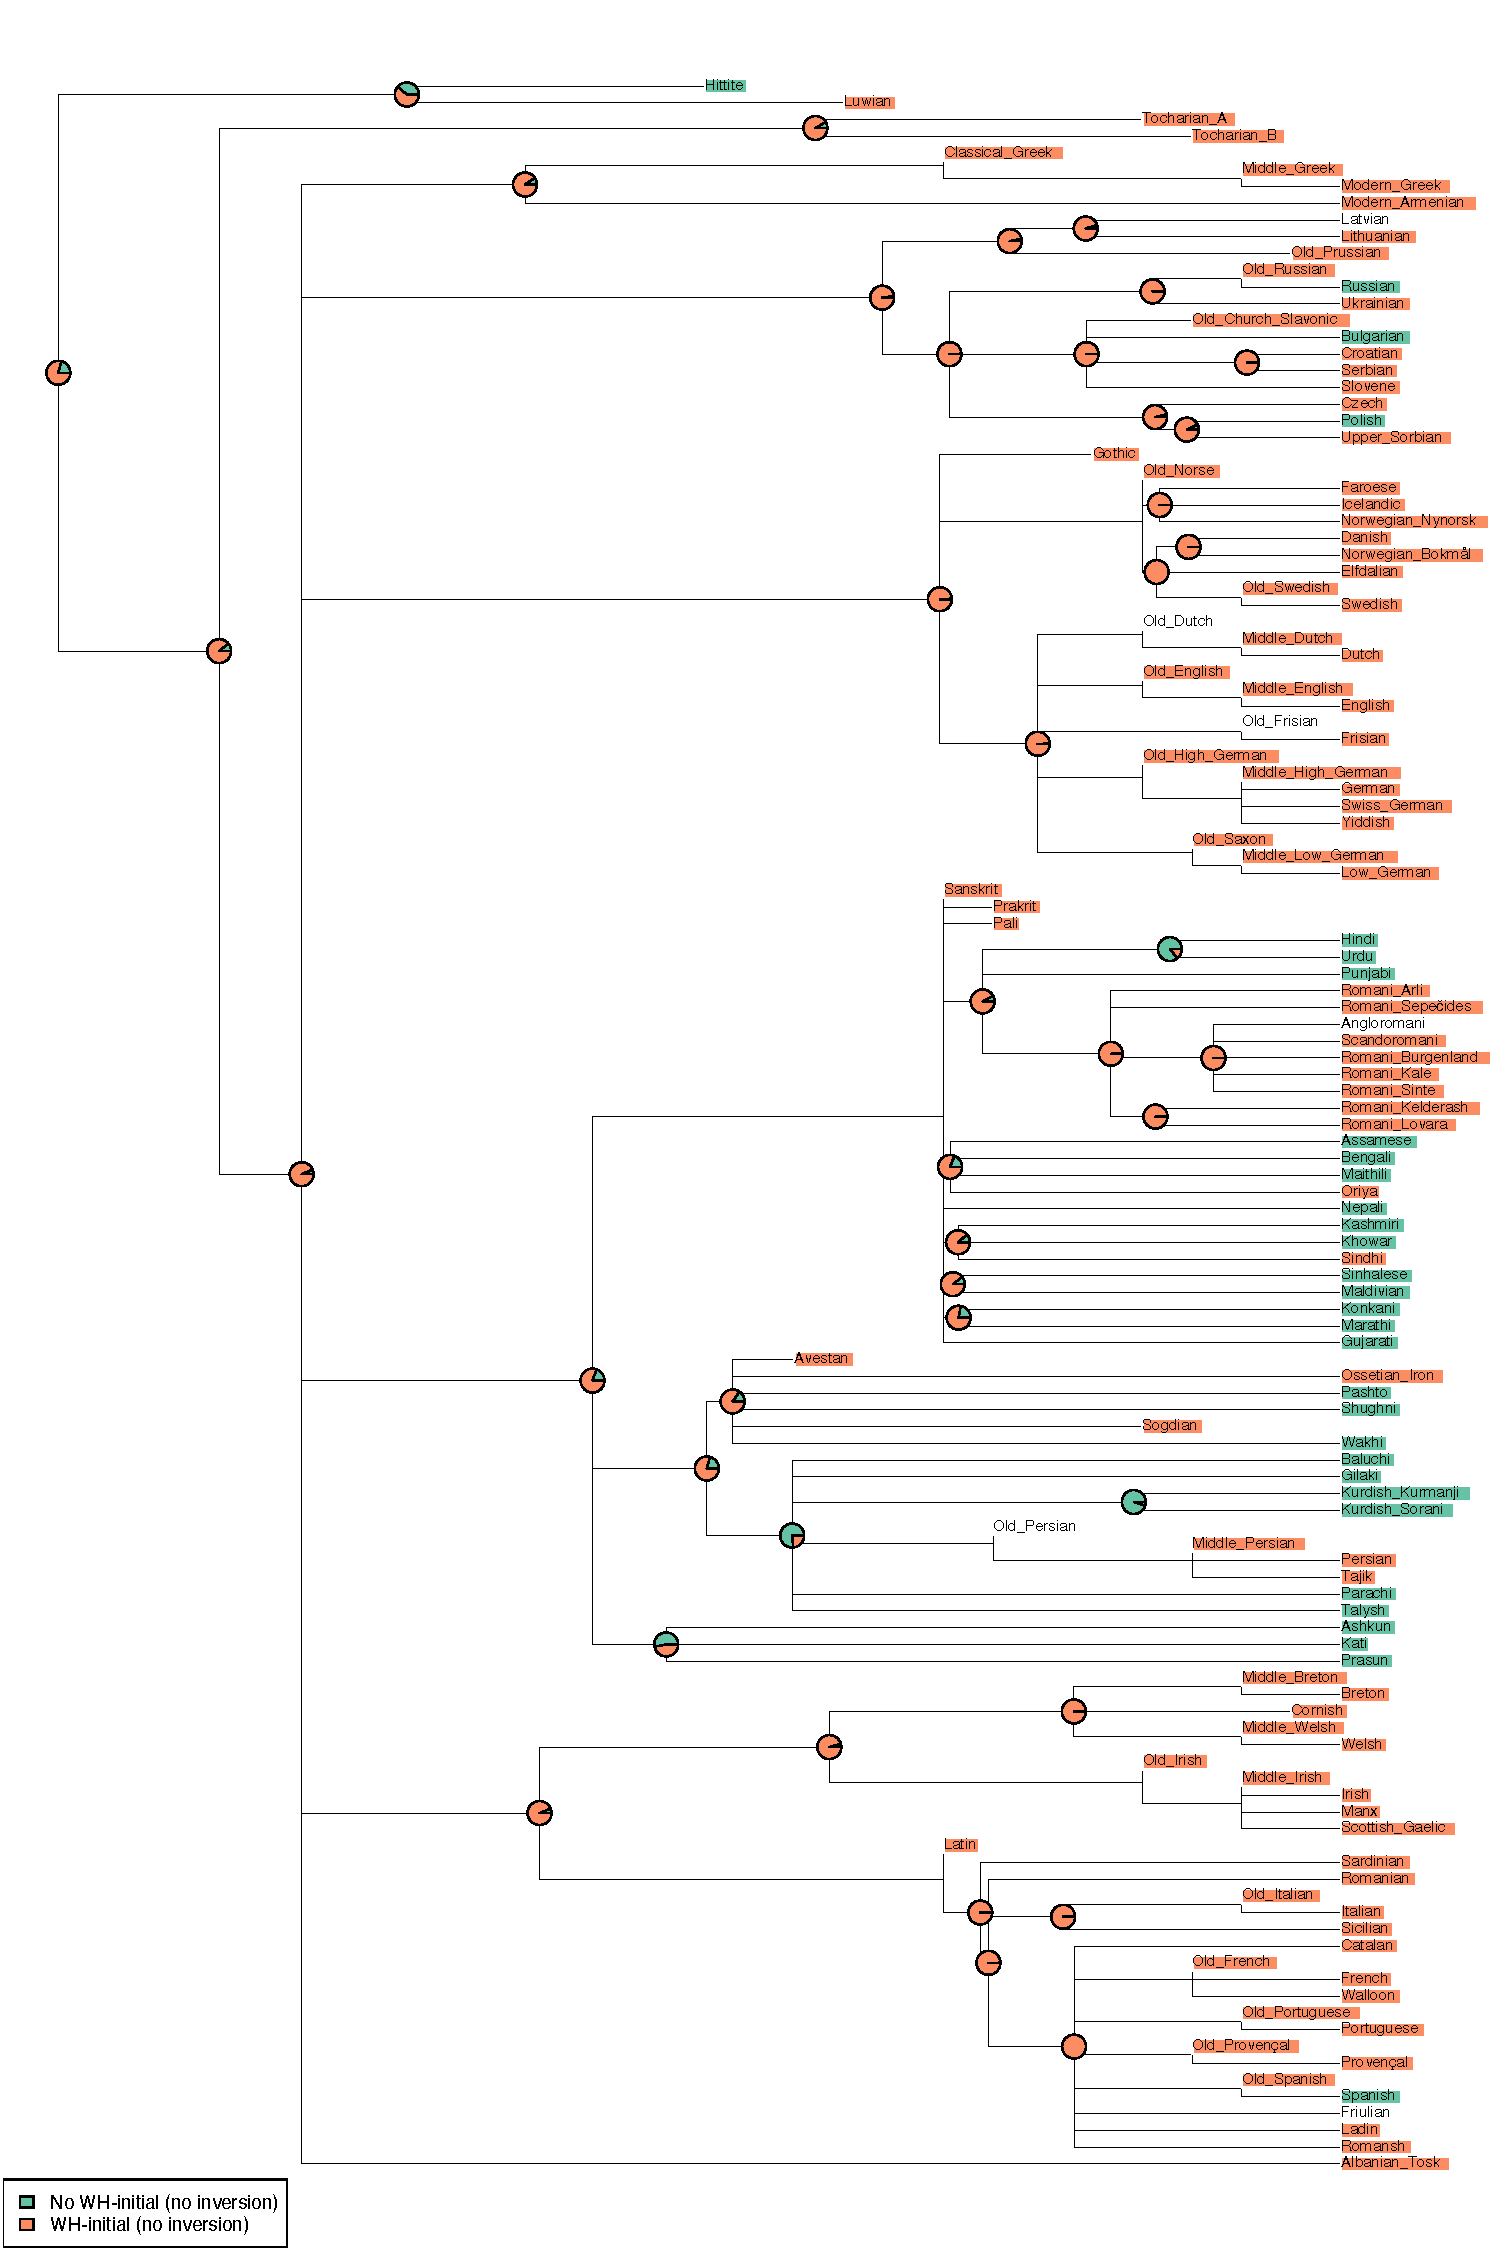
\includegraphics{supp-graphics/Word.order.WH.element.WH.initial.pdf}
%\end{figure}

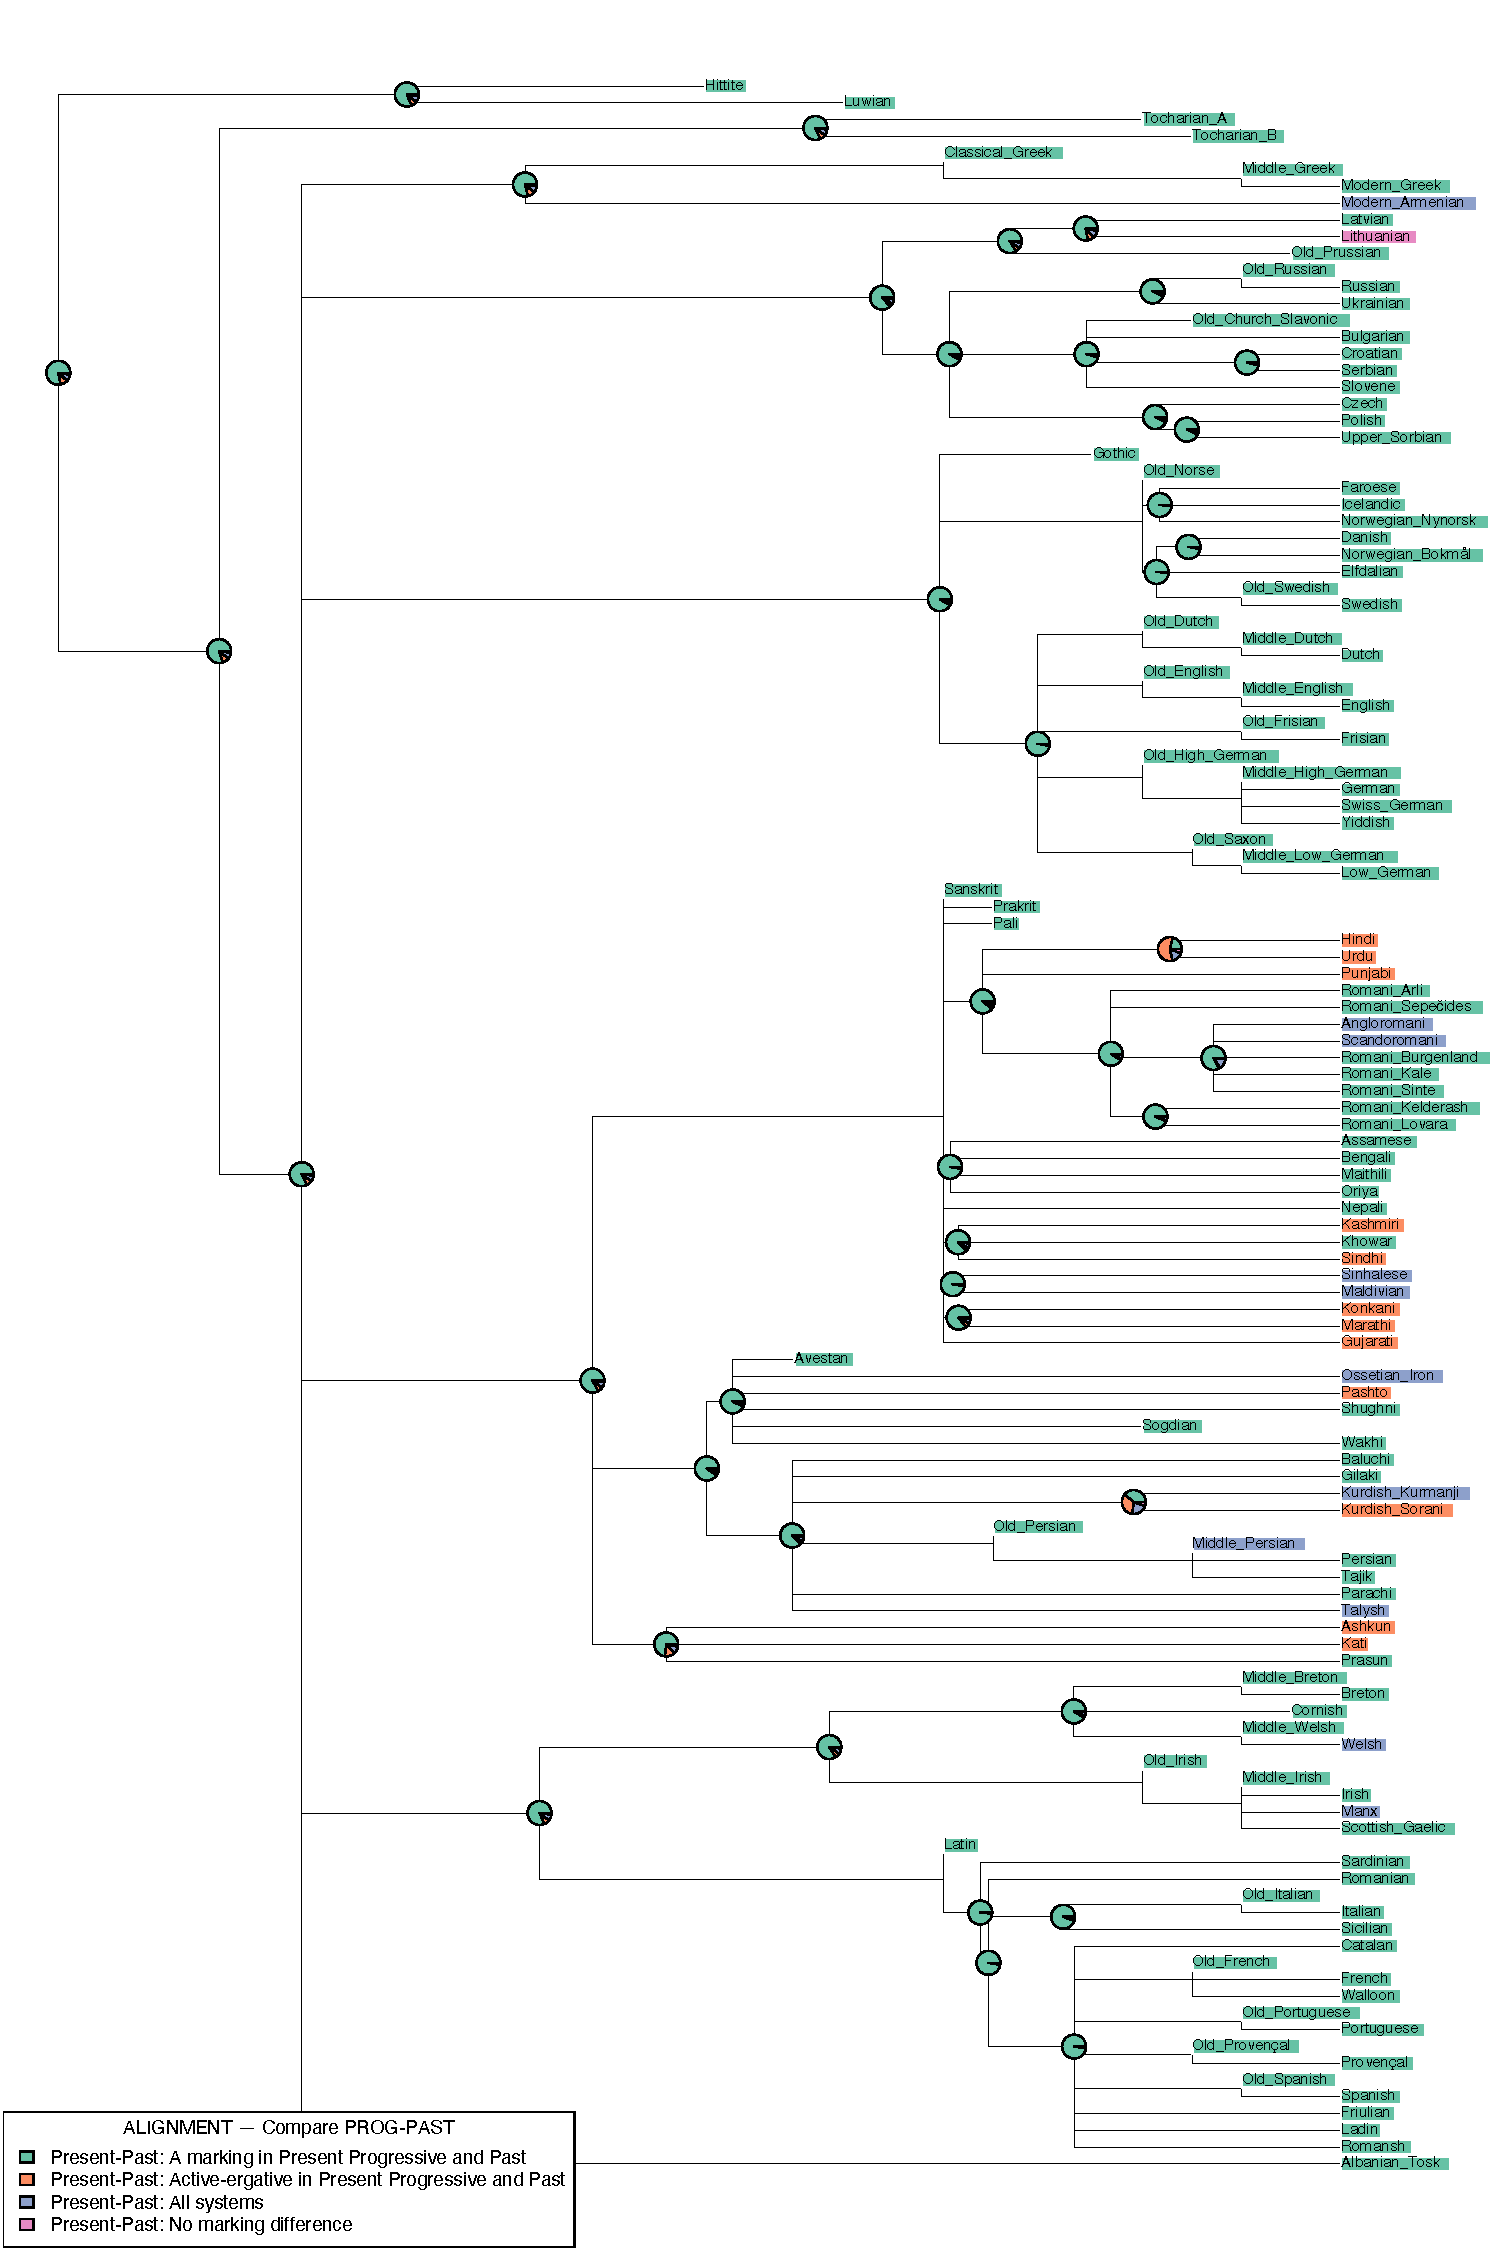
\includegraphics[width=.9\linewidth]{supp-graphics/ALIGNMENTComparePROGPASTPAST-APROG-OALIGNMENTComparePROGPASTPROG-APST-OALIGNMENTComparePROGPASTPROG-SoPST-So.pdf}

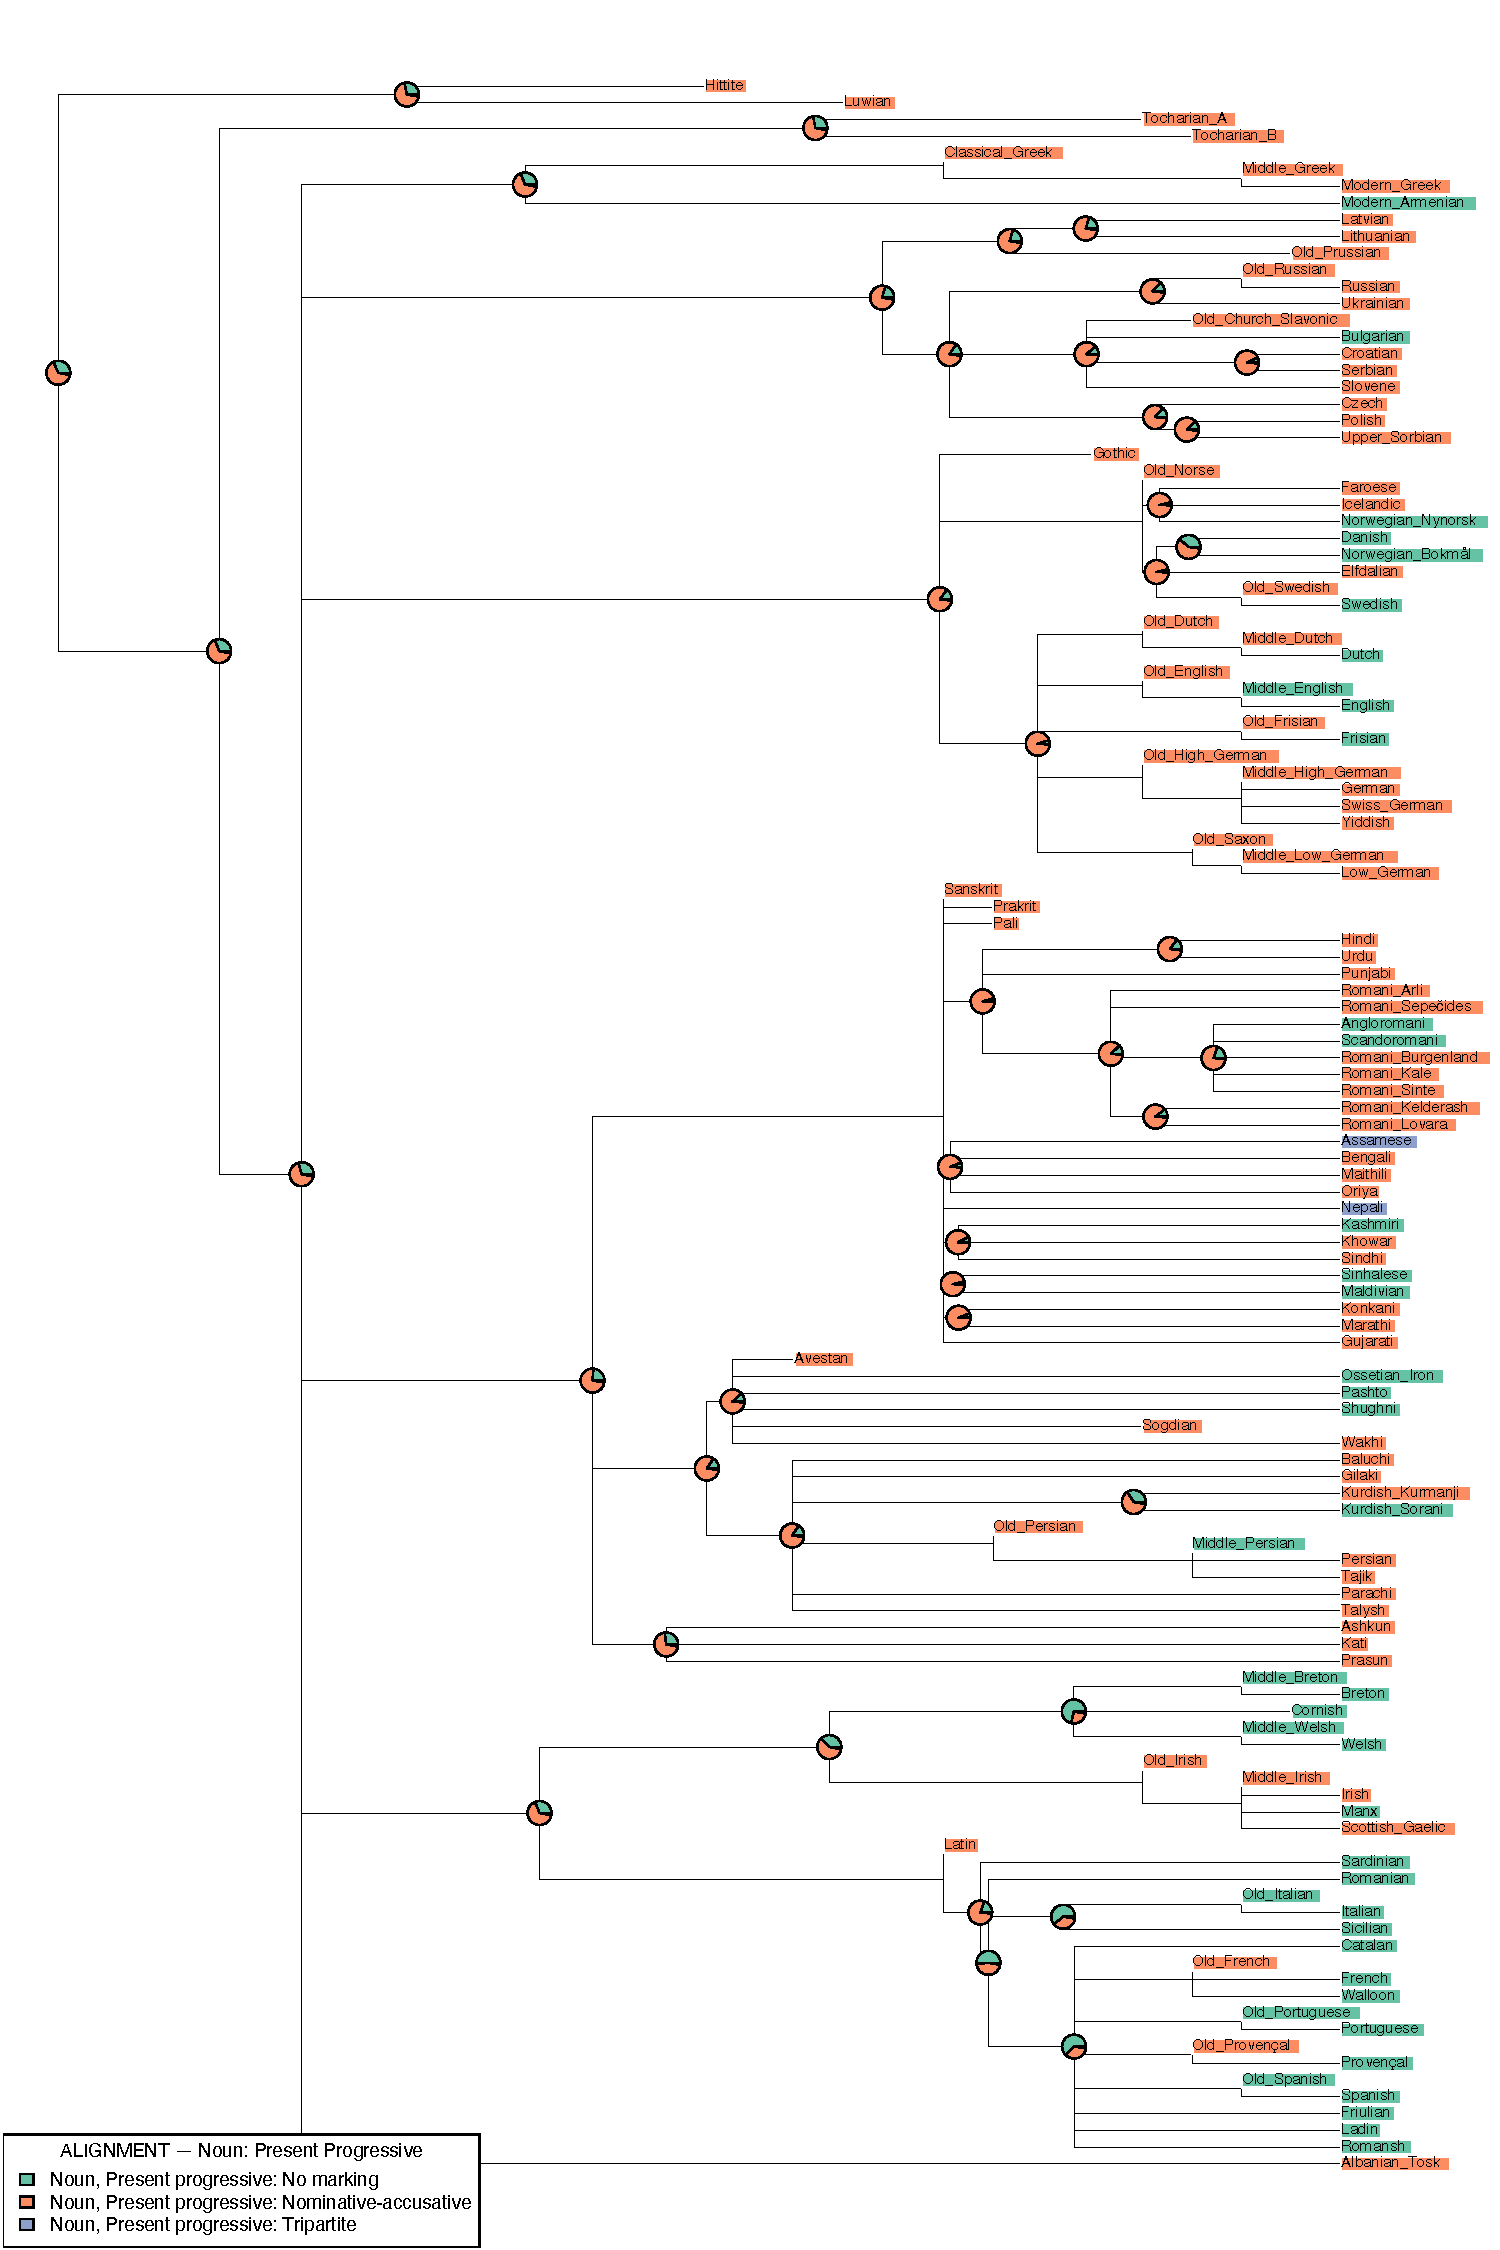
\includegraphics[width=.9\linewidth]{supp-graphics/ALIGNMENTNounPresentProgressiveNPROGOSoALIGNMENTNounPresentProgressiveNPROGAOALIGNMENTNounPresentProgressiveNPROGASaALIGNMENTNounPresentProgressiveNPROGSaSo.pdf}

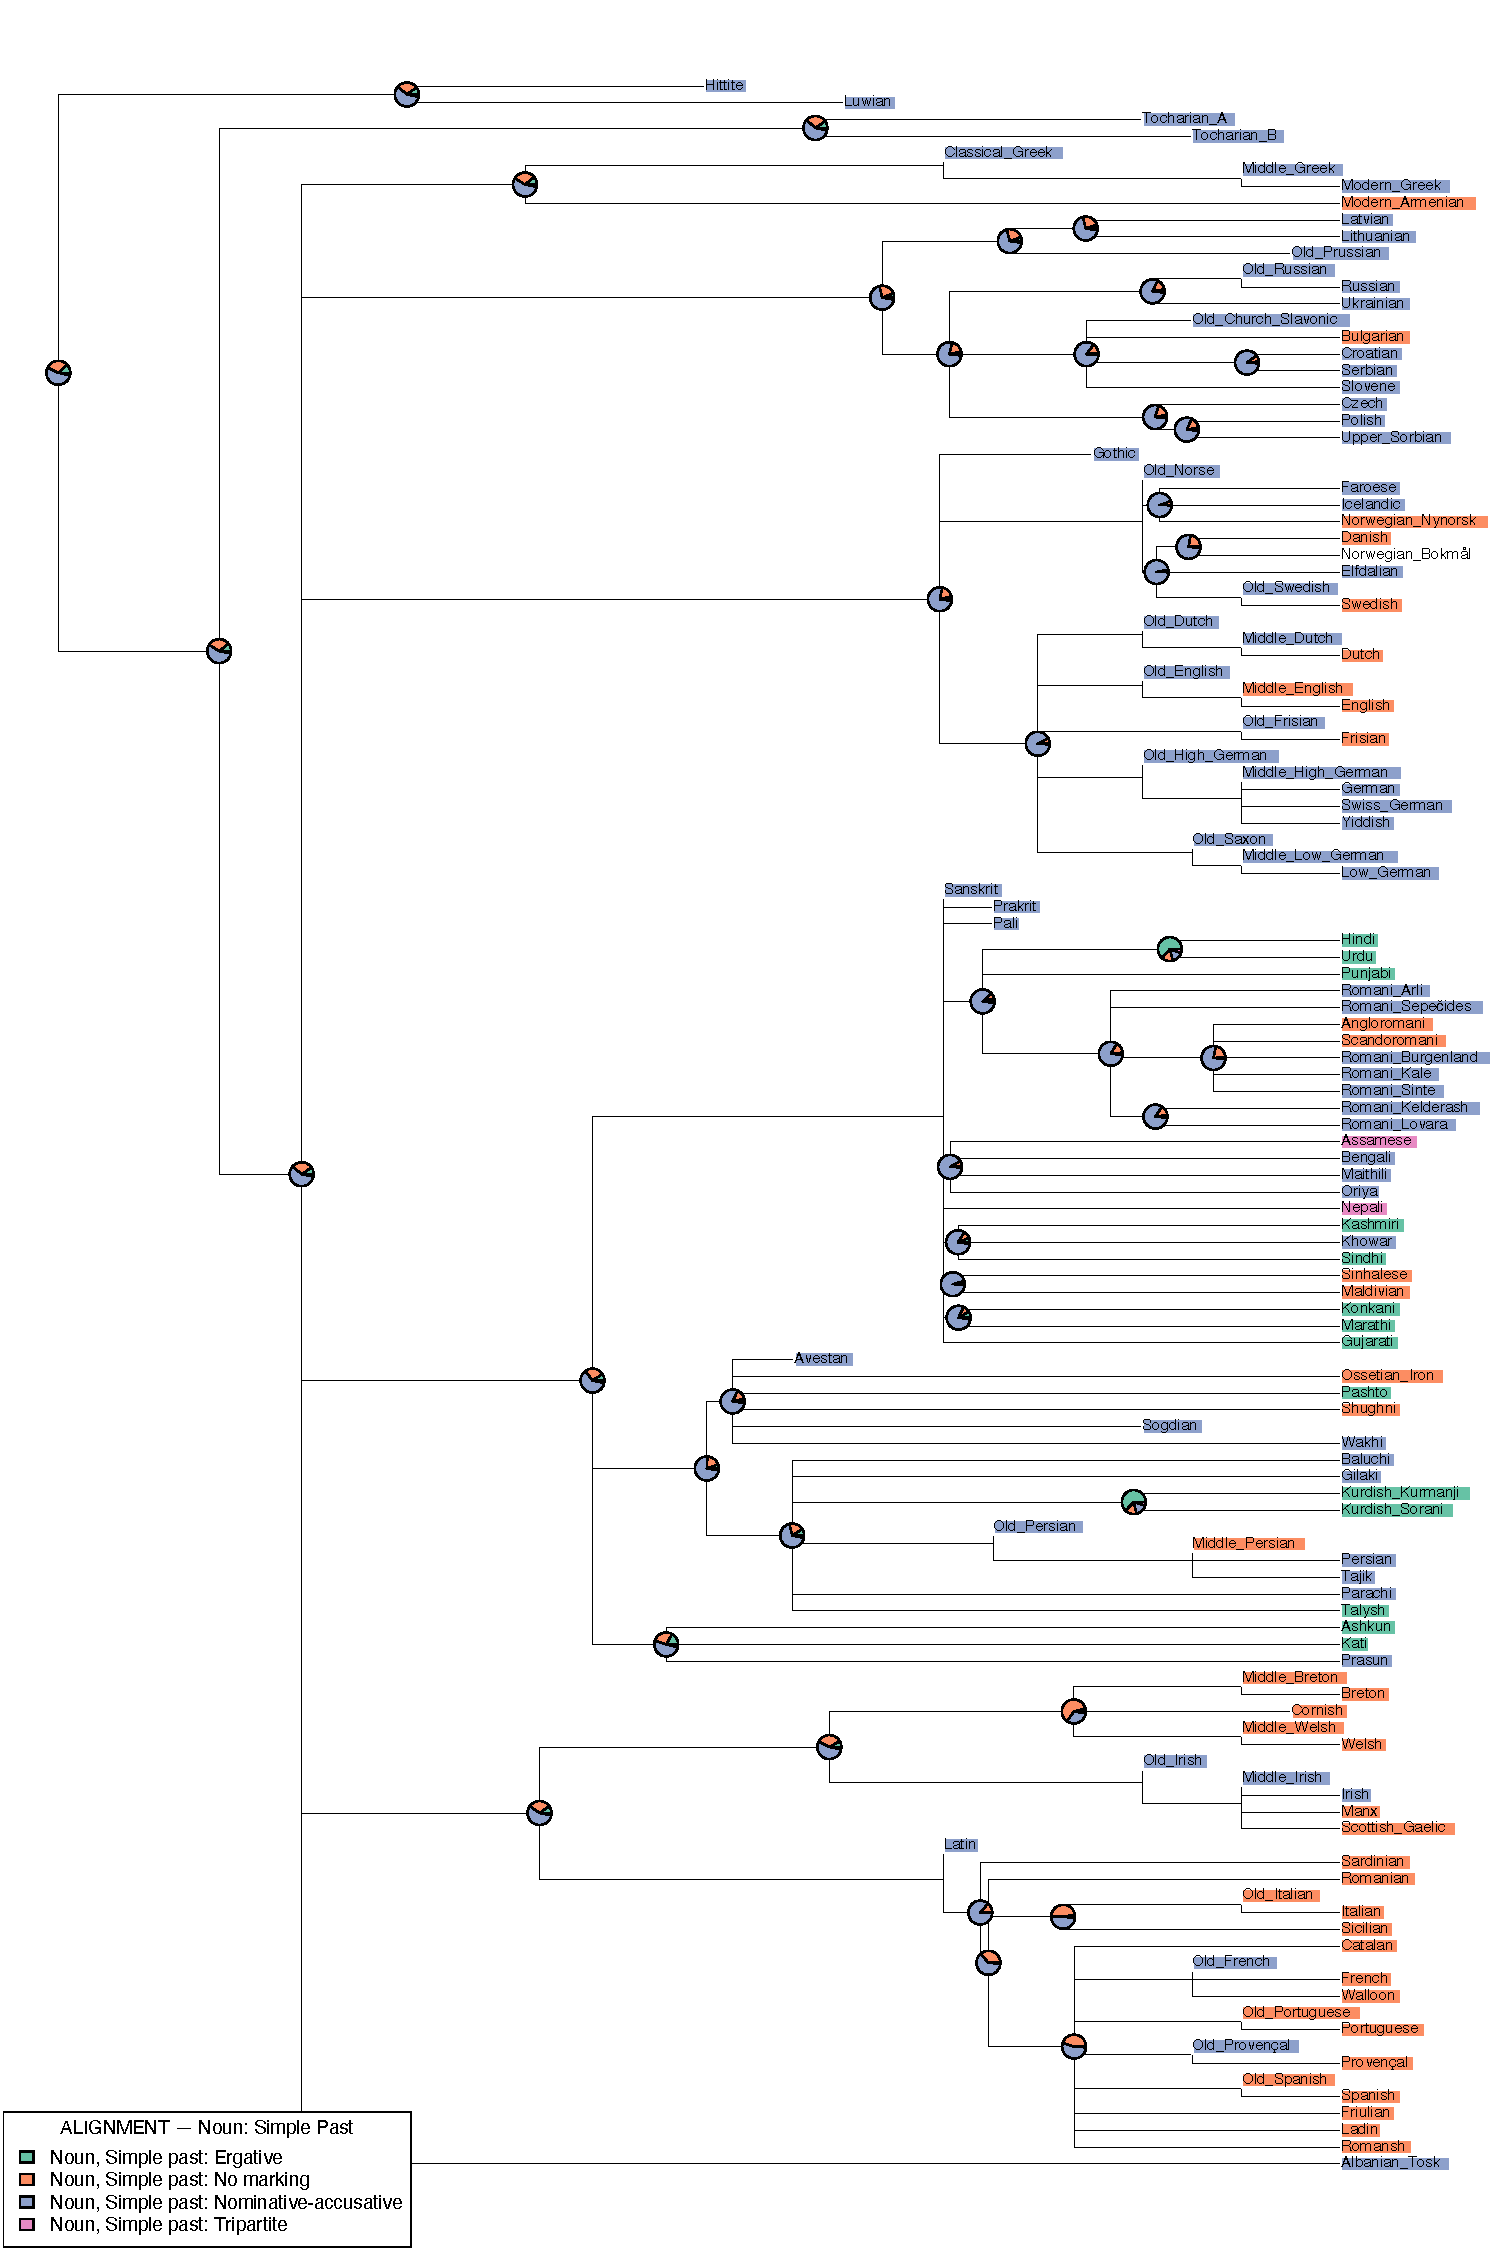
\includegraphics[width=.9\linewidth]{supp-graphics/ALIGNMENTNounSimplePastNPSTOSoALIGNMENTNounSimplePastNPSTAOALIGNMENTNounSimplePastNPSTASaALIGNMENTNounSimplePastNPSTSaSo.pdf}

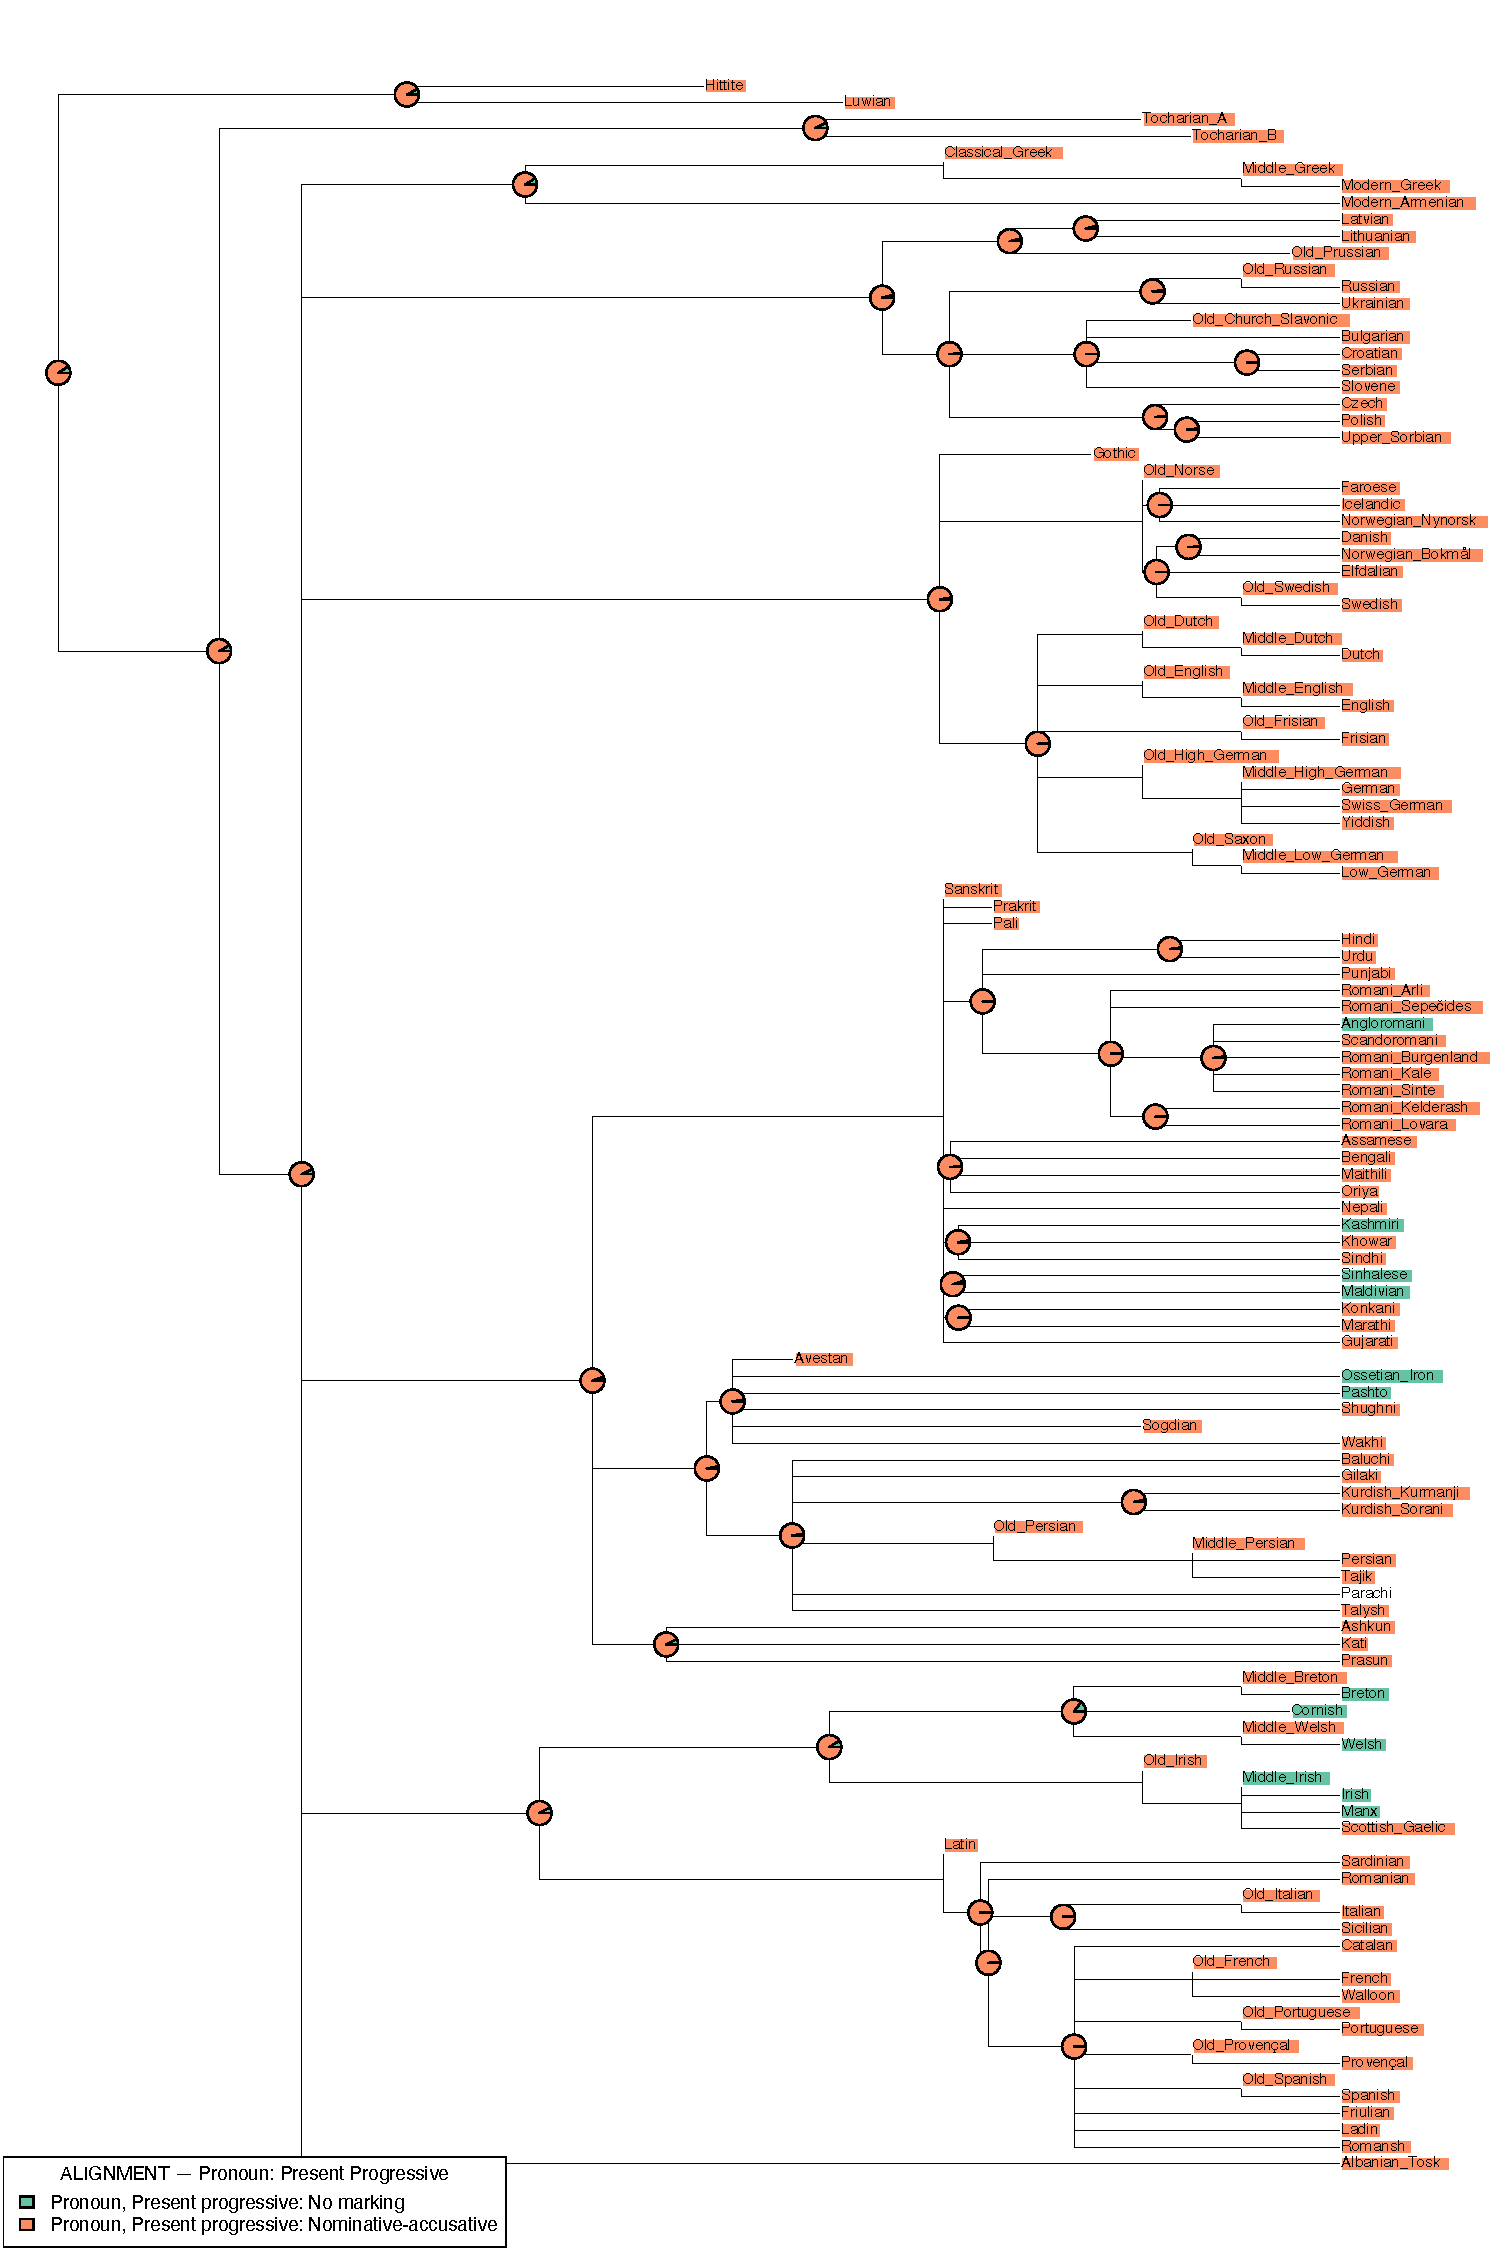
\includegraphics[width=.9\linewidth]{supp-graphics/ALIGNMENTPronounPresentProgressivePPROGOSoALIGNMENTPronounPresentProgressivePPROGAOALIGNMENTPronounPresentProgressivePPROGASaALIGNMENTPronounPresentProgressivePPROGSaSo.pdf}

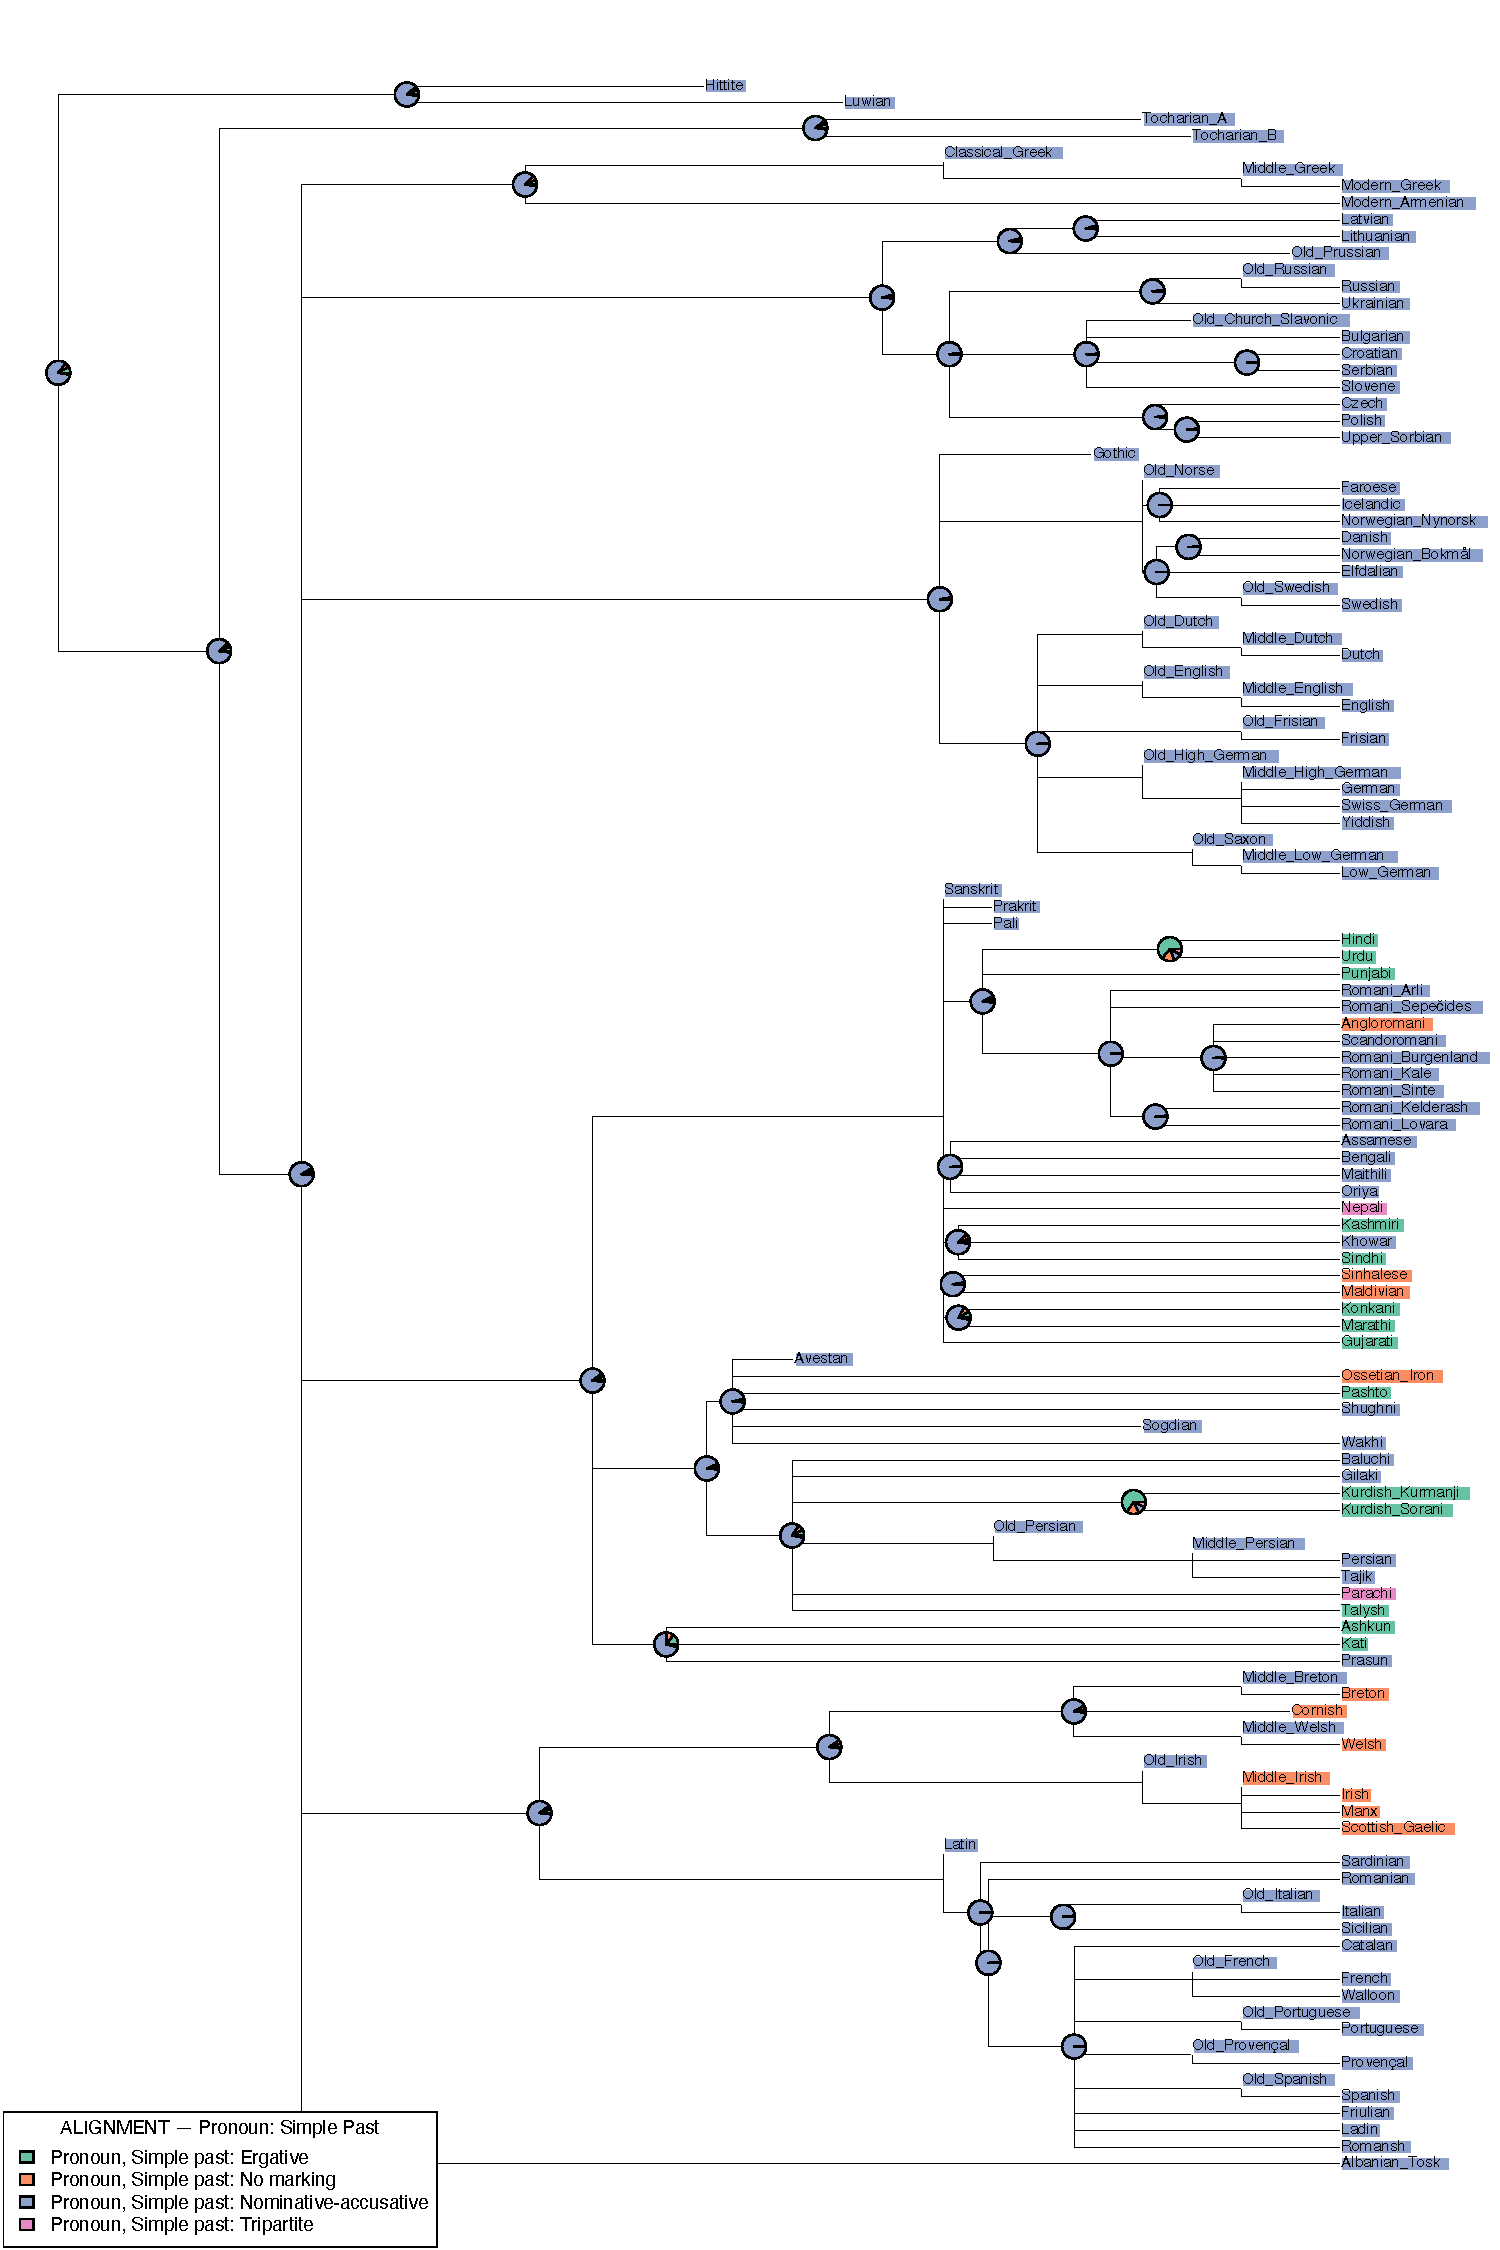
\includegraphics[width=.9\linewidth]{supp-graphics/ALIGNMENTPronounSimplePastPPSTOSoALIGNMENTPronounSimplePastPPSTAOALIGNMENTPronounSimplePastPPSTASaALIGNMENTPronounSimplePastPPSTSaSo.pdf}

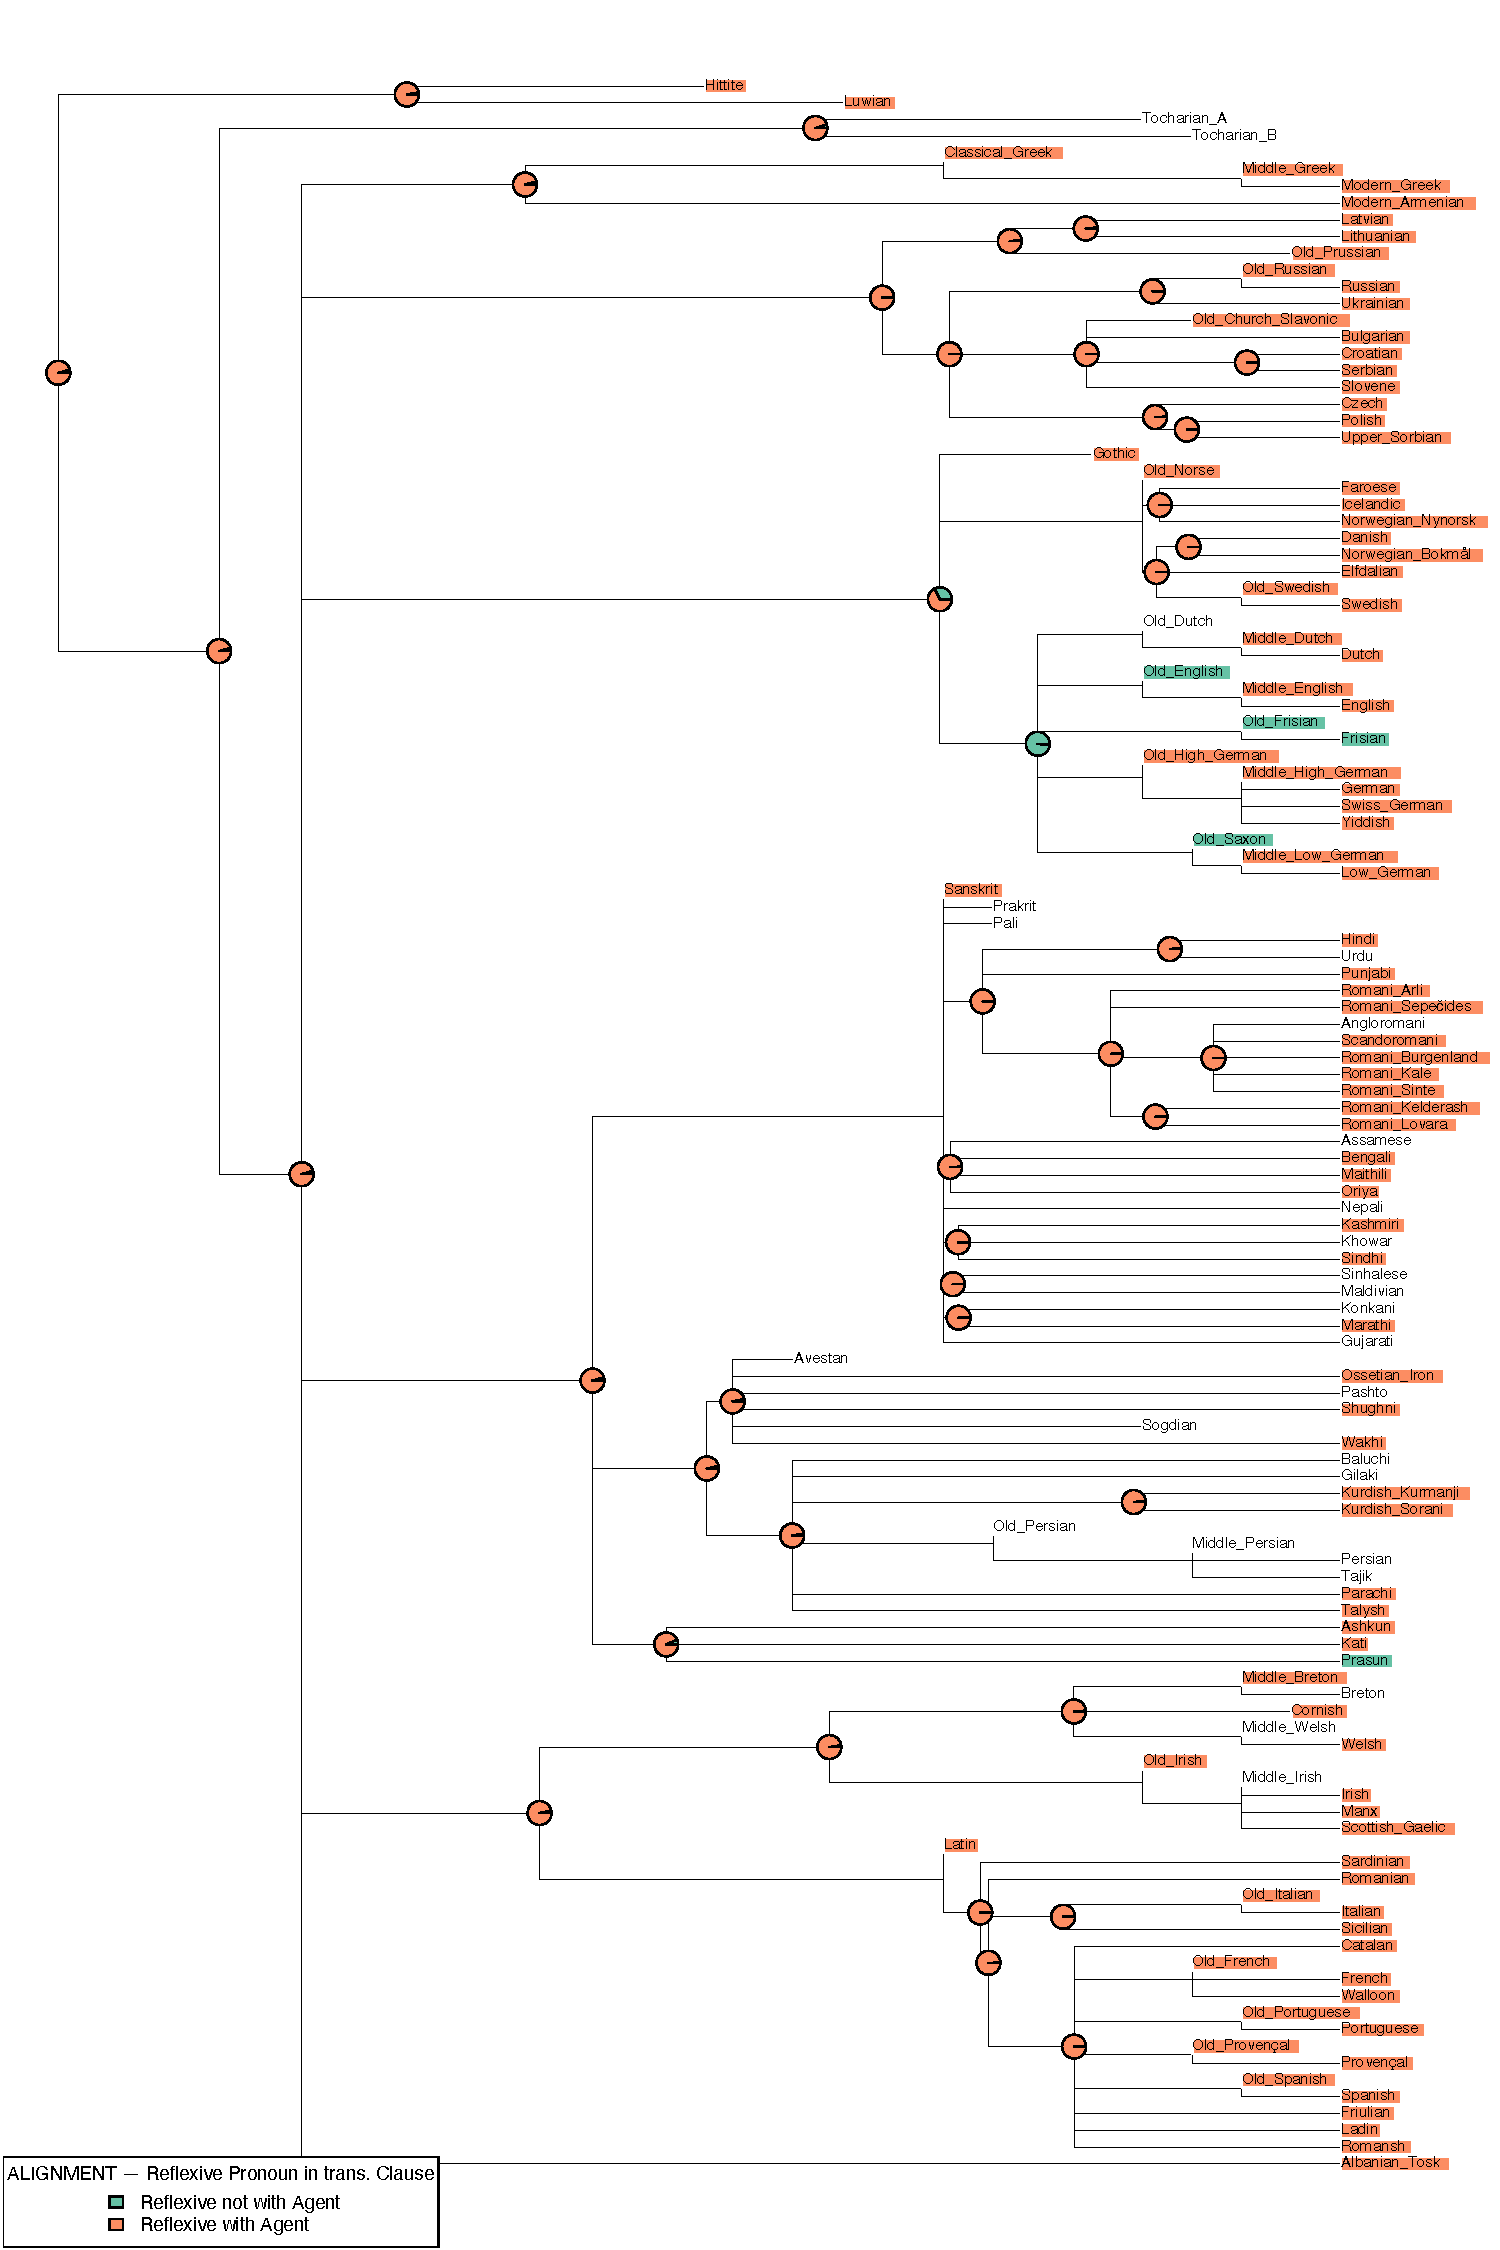
\includegraphics[width=.9\linewidth]{supp-graphics/ALIGNMENTReflexivePronounintransClauseREFLrefA.pdf}

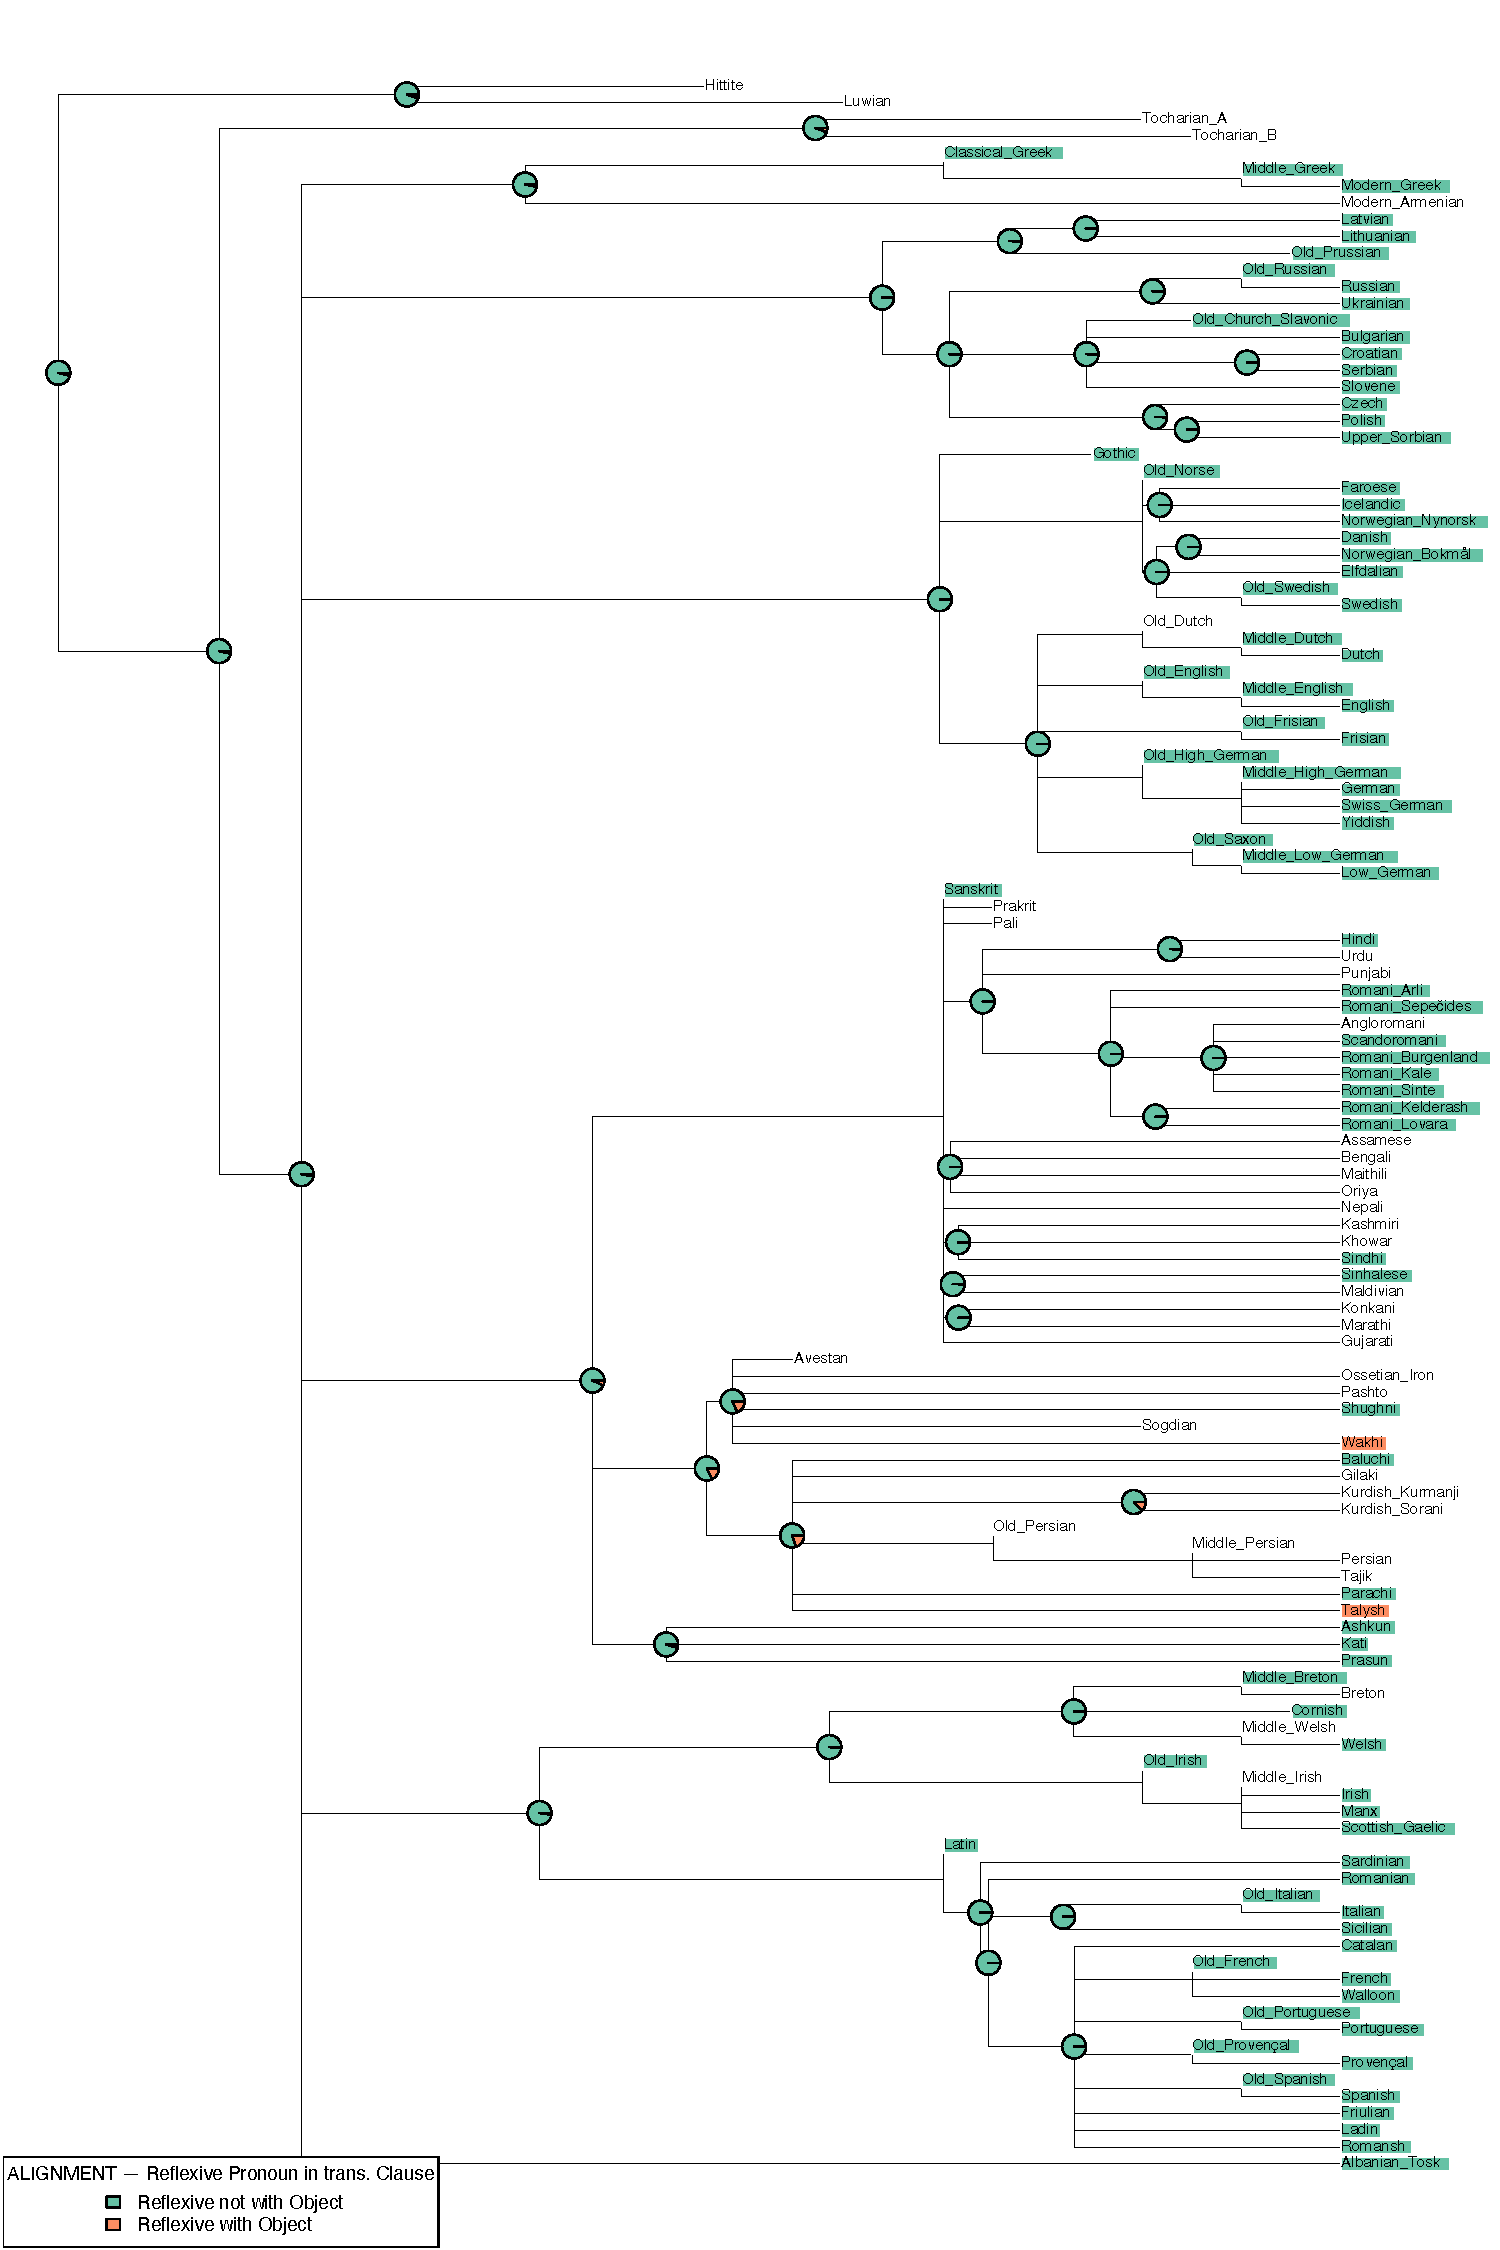
\includegraphics[width=.9\linewidth]{supp-graphics/ALIGNMENTReflexivePronounintransClauseREFLrefO.pdf}

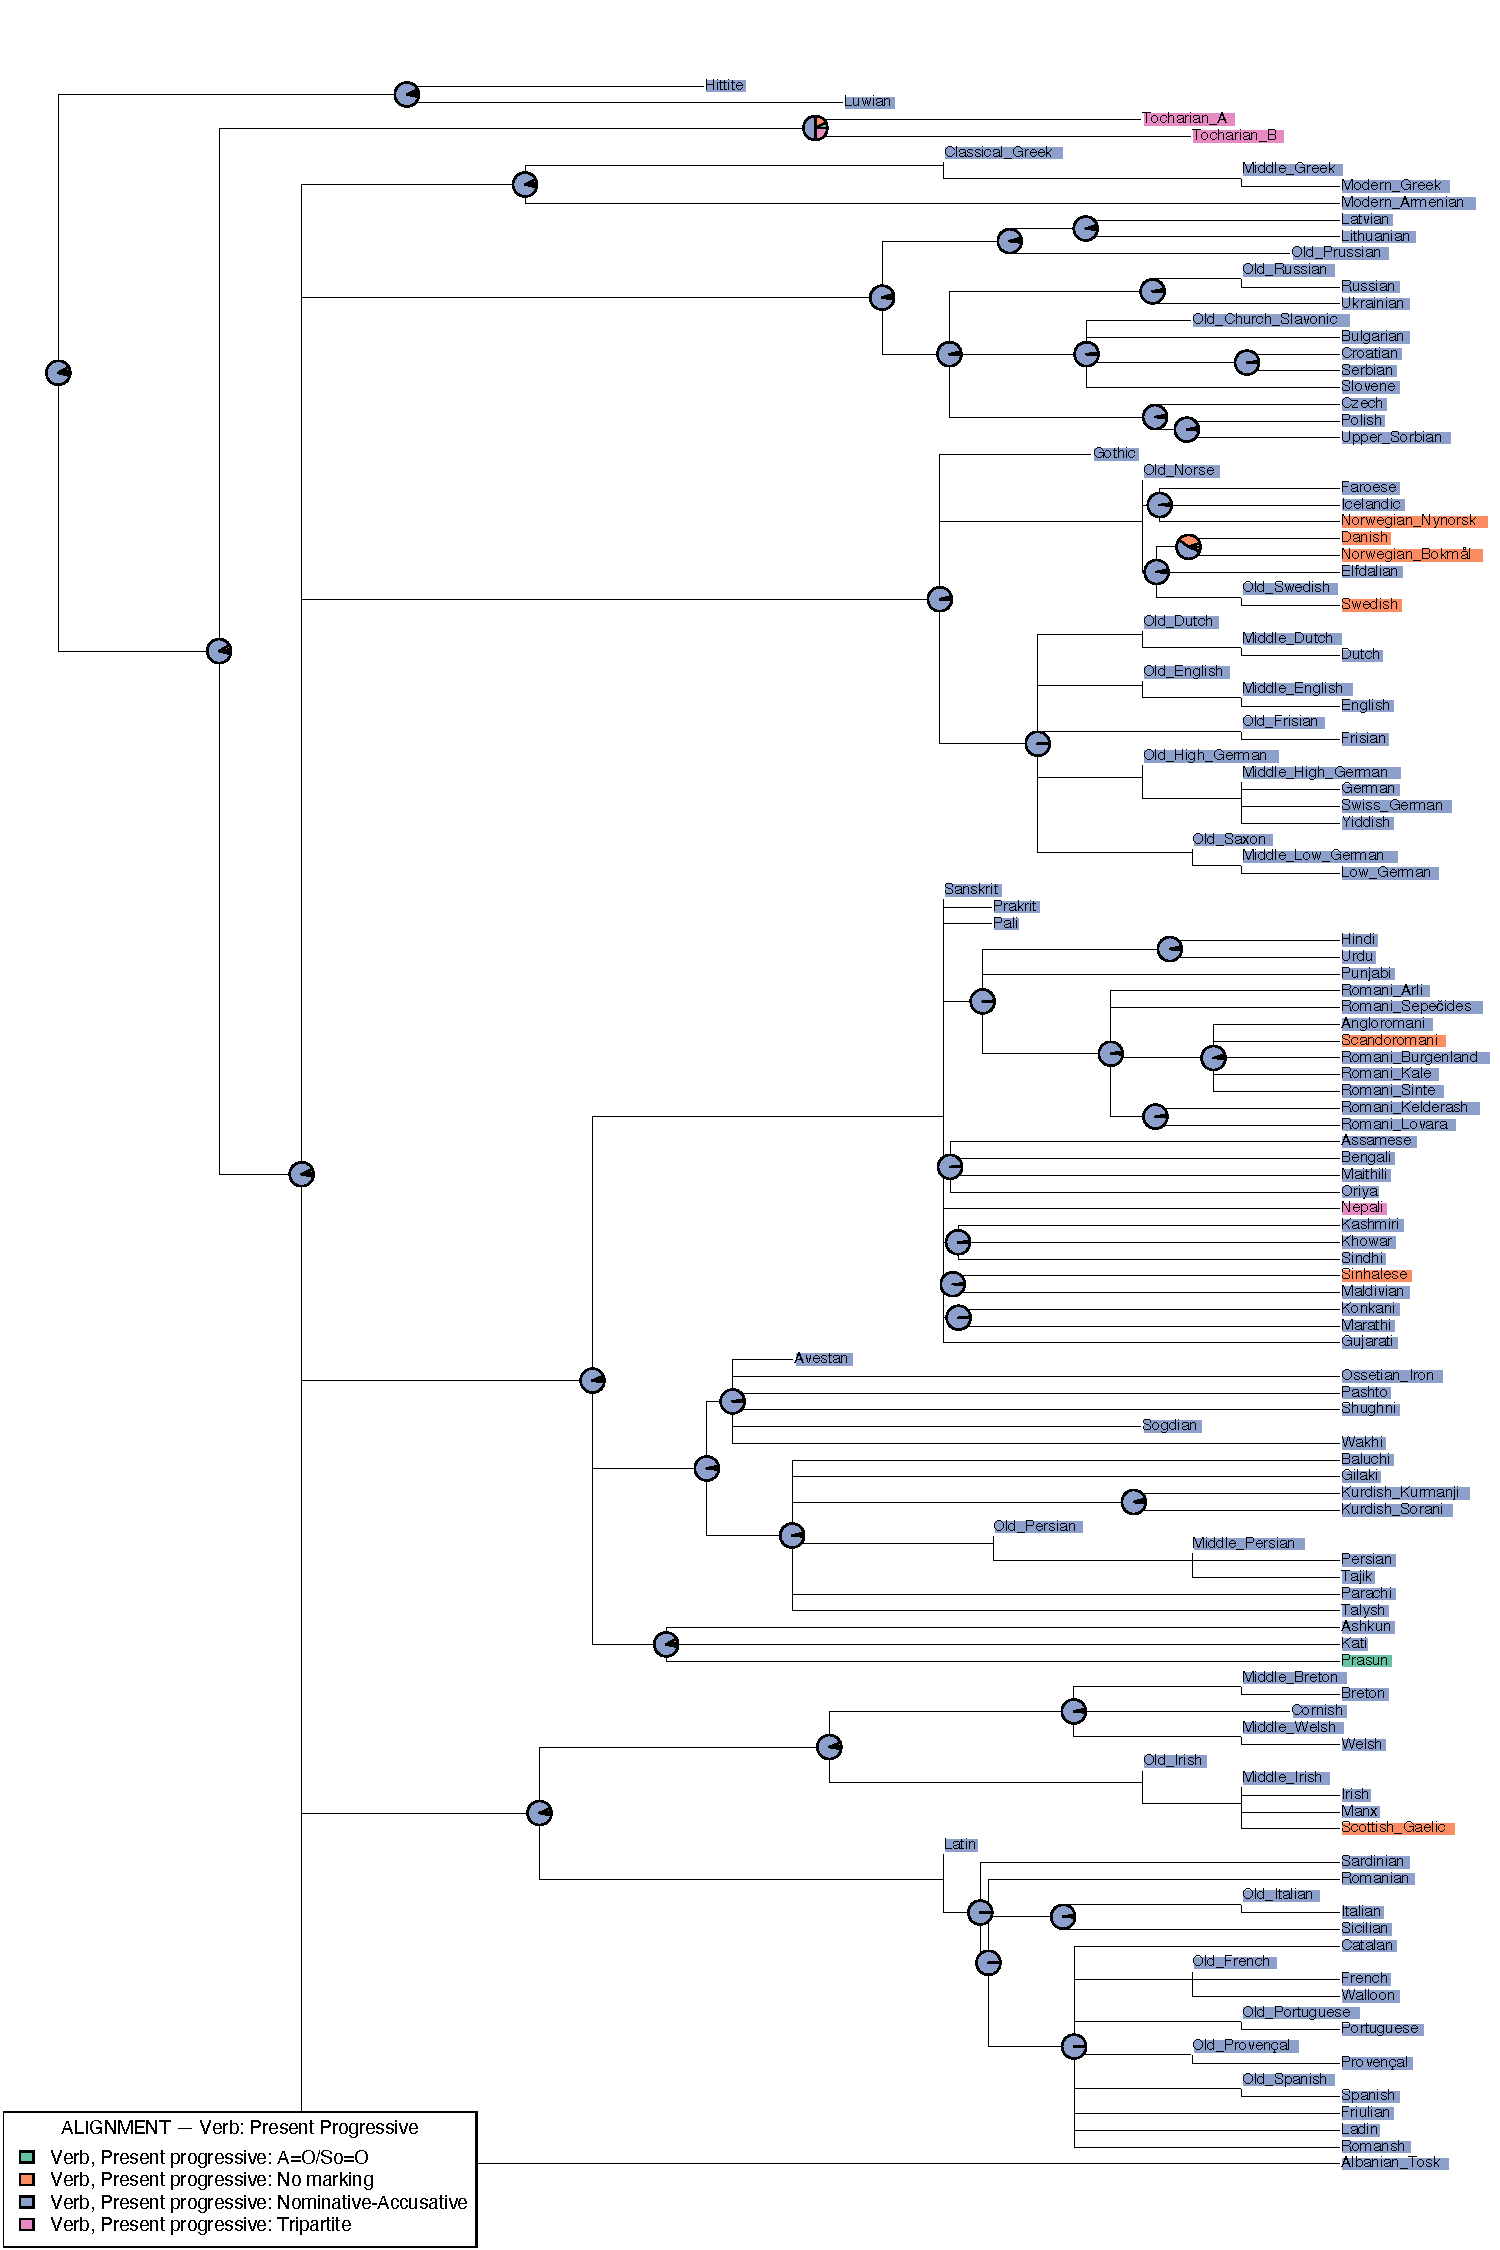
\includegraphics[width=.9\linewidth]{supp-graphics/ALIGNMENTVerbPresentProgressiveVPROGOSoALIGNMENTVerbPresentProgressiveVPROGAOALIGNMENTVerbPresentProgressiveVPROGASaALIGNMENTVerbPresentProgressiveVPROGSaSo.pdf}

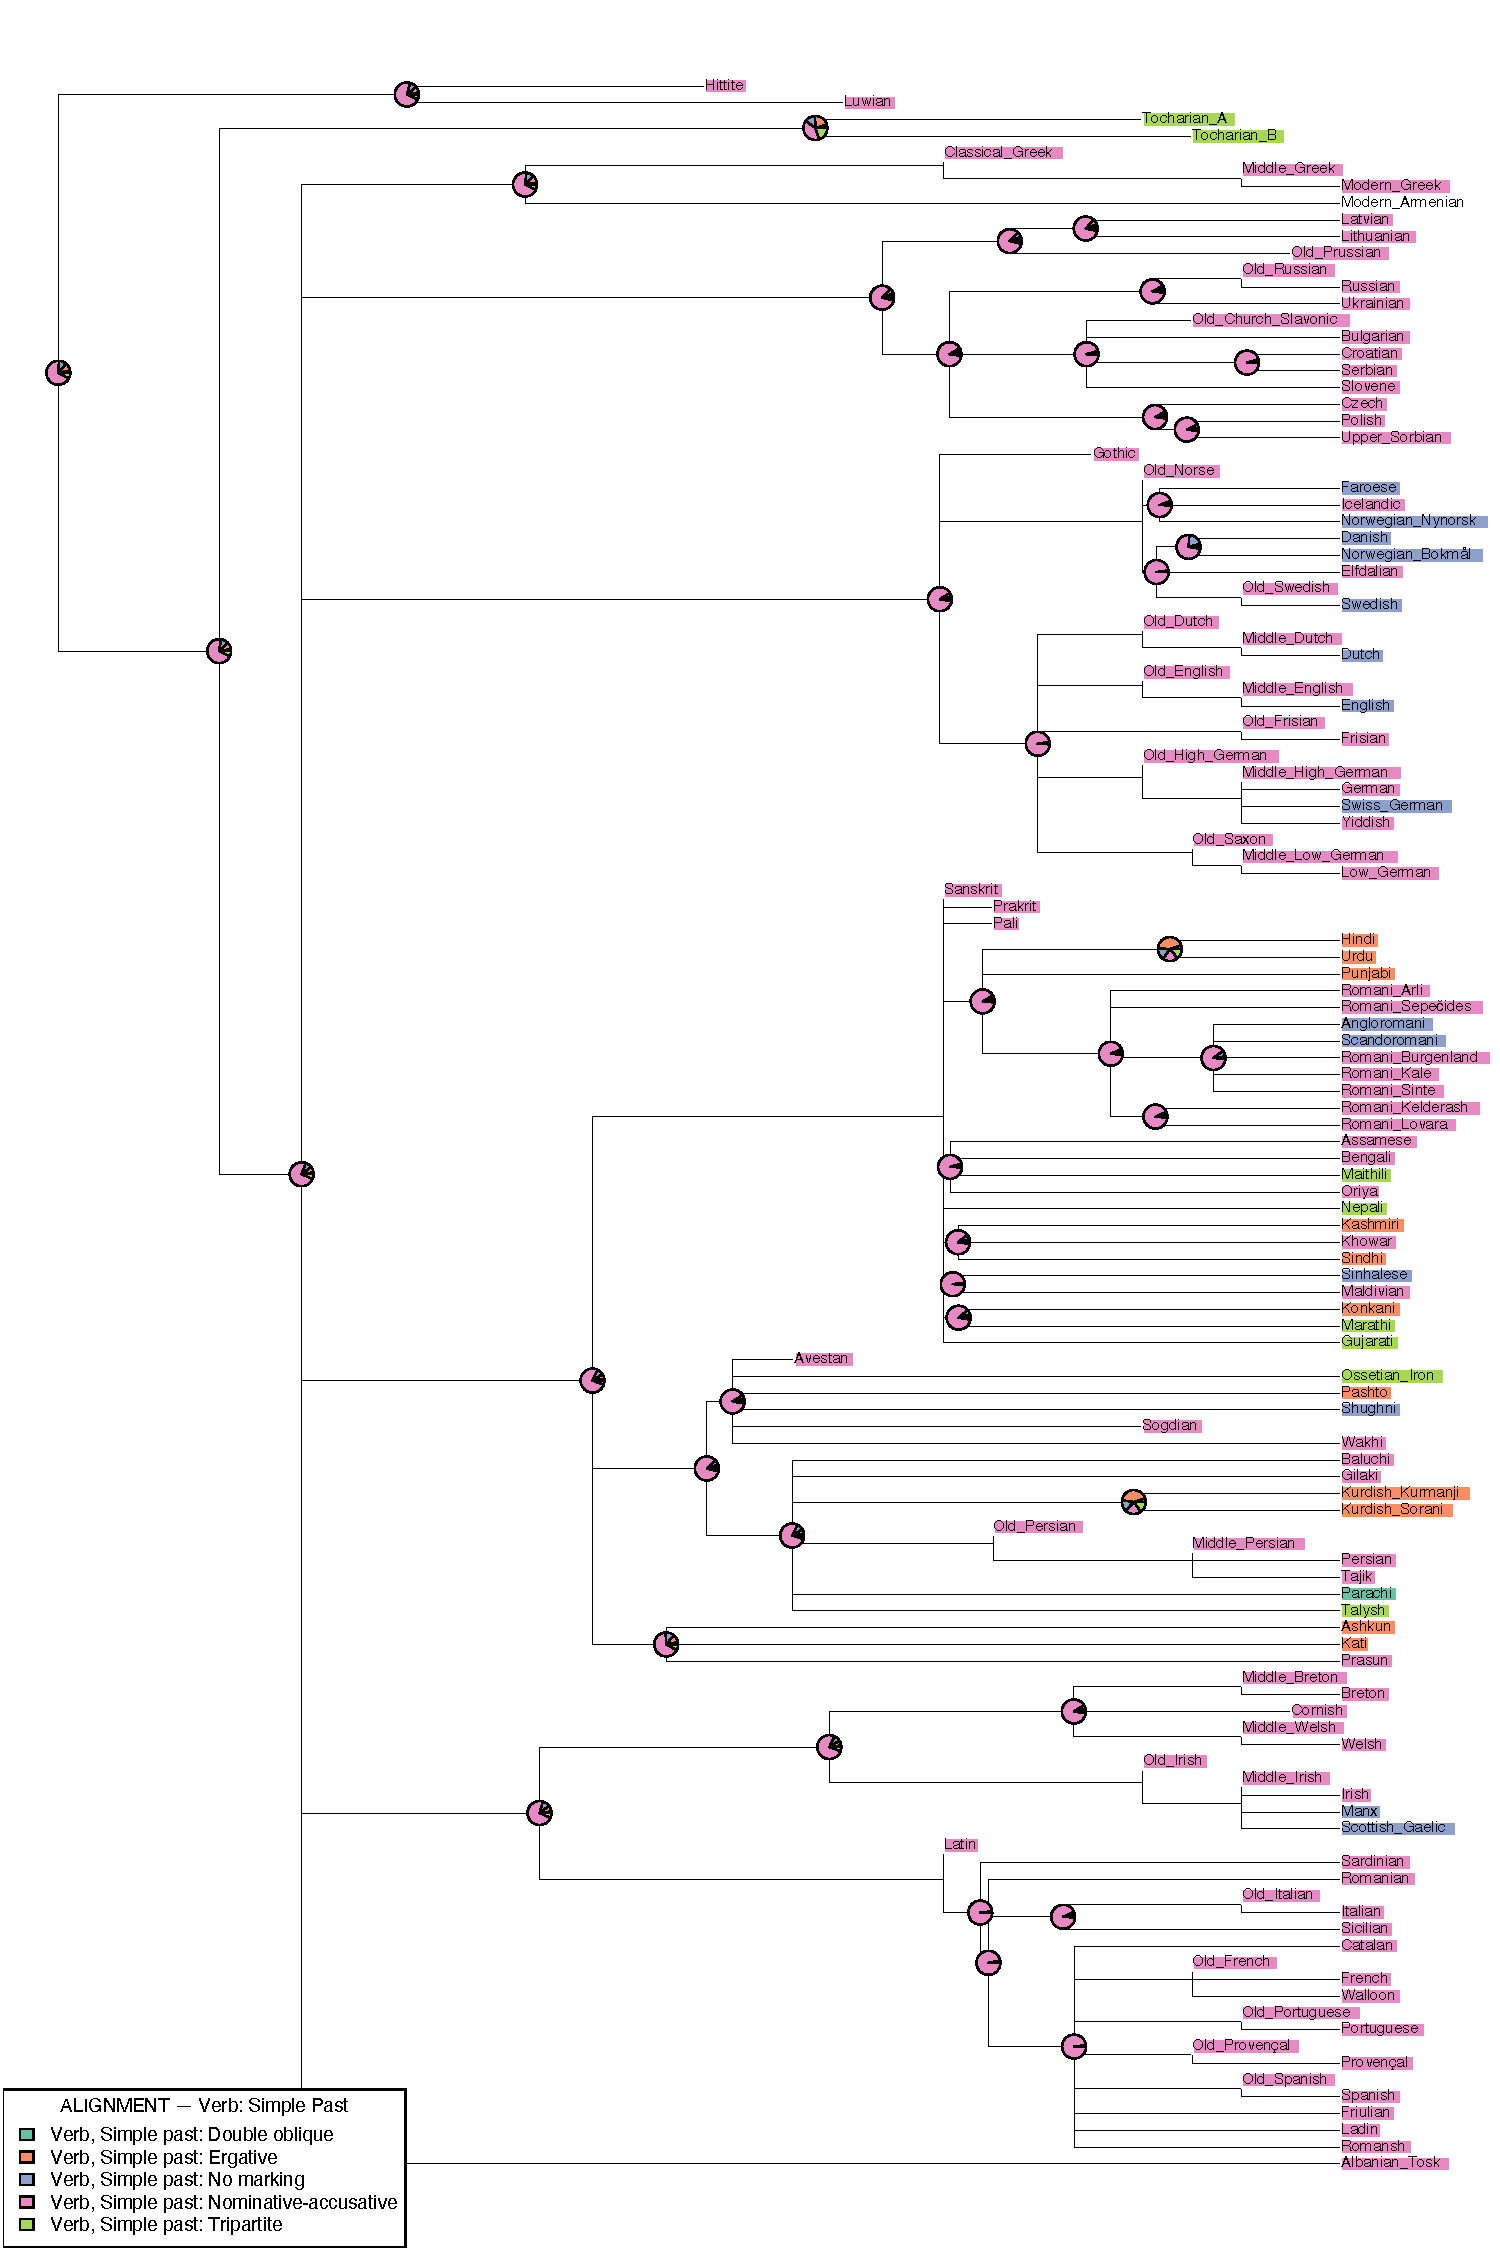
\includegraphics[width=.9\linewidth]{supp-graphics/ALIGNMENTVerbSimplePastVPSTOSoALIGNMENTVerbSimplePastVPSTAOALIGNMENTVerbSimplePastVPSTASaALIGNMENTVerbSimplePastVPSTSaSo.pdf}

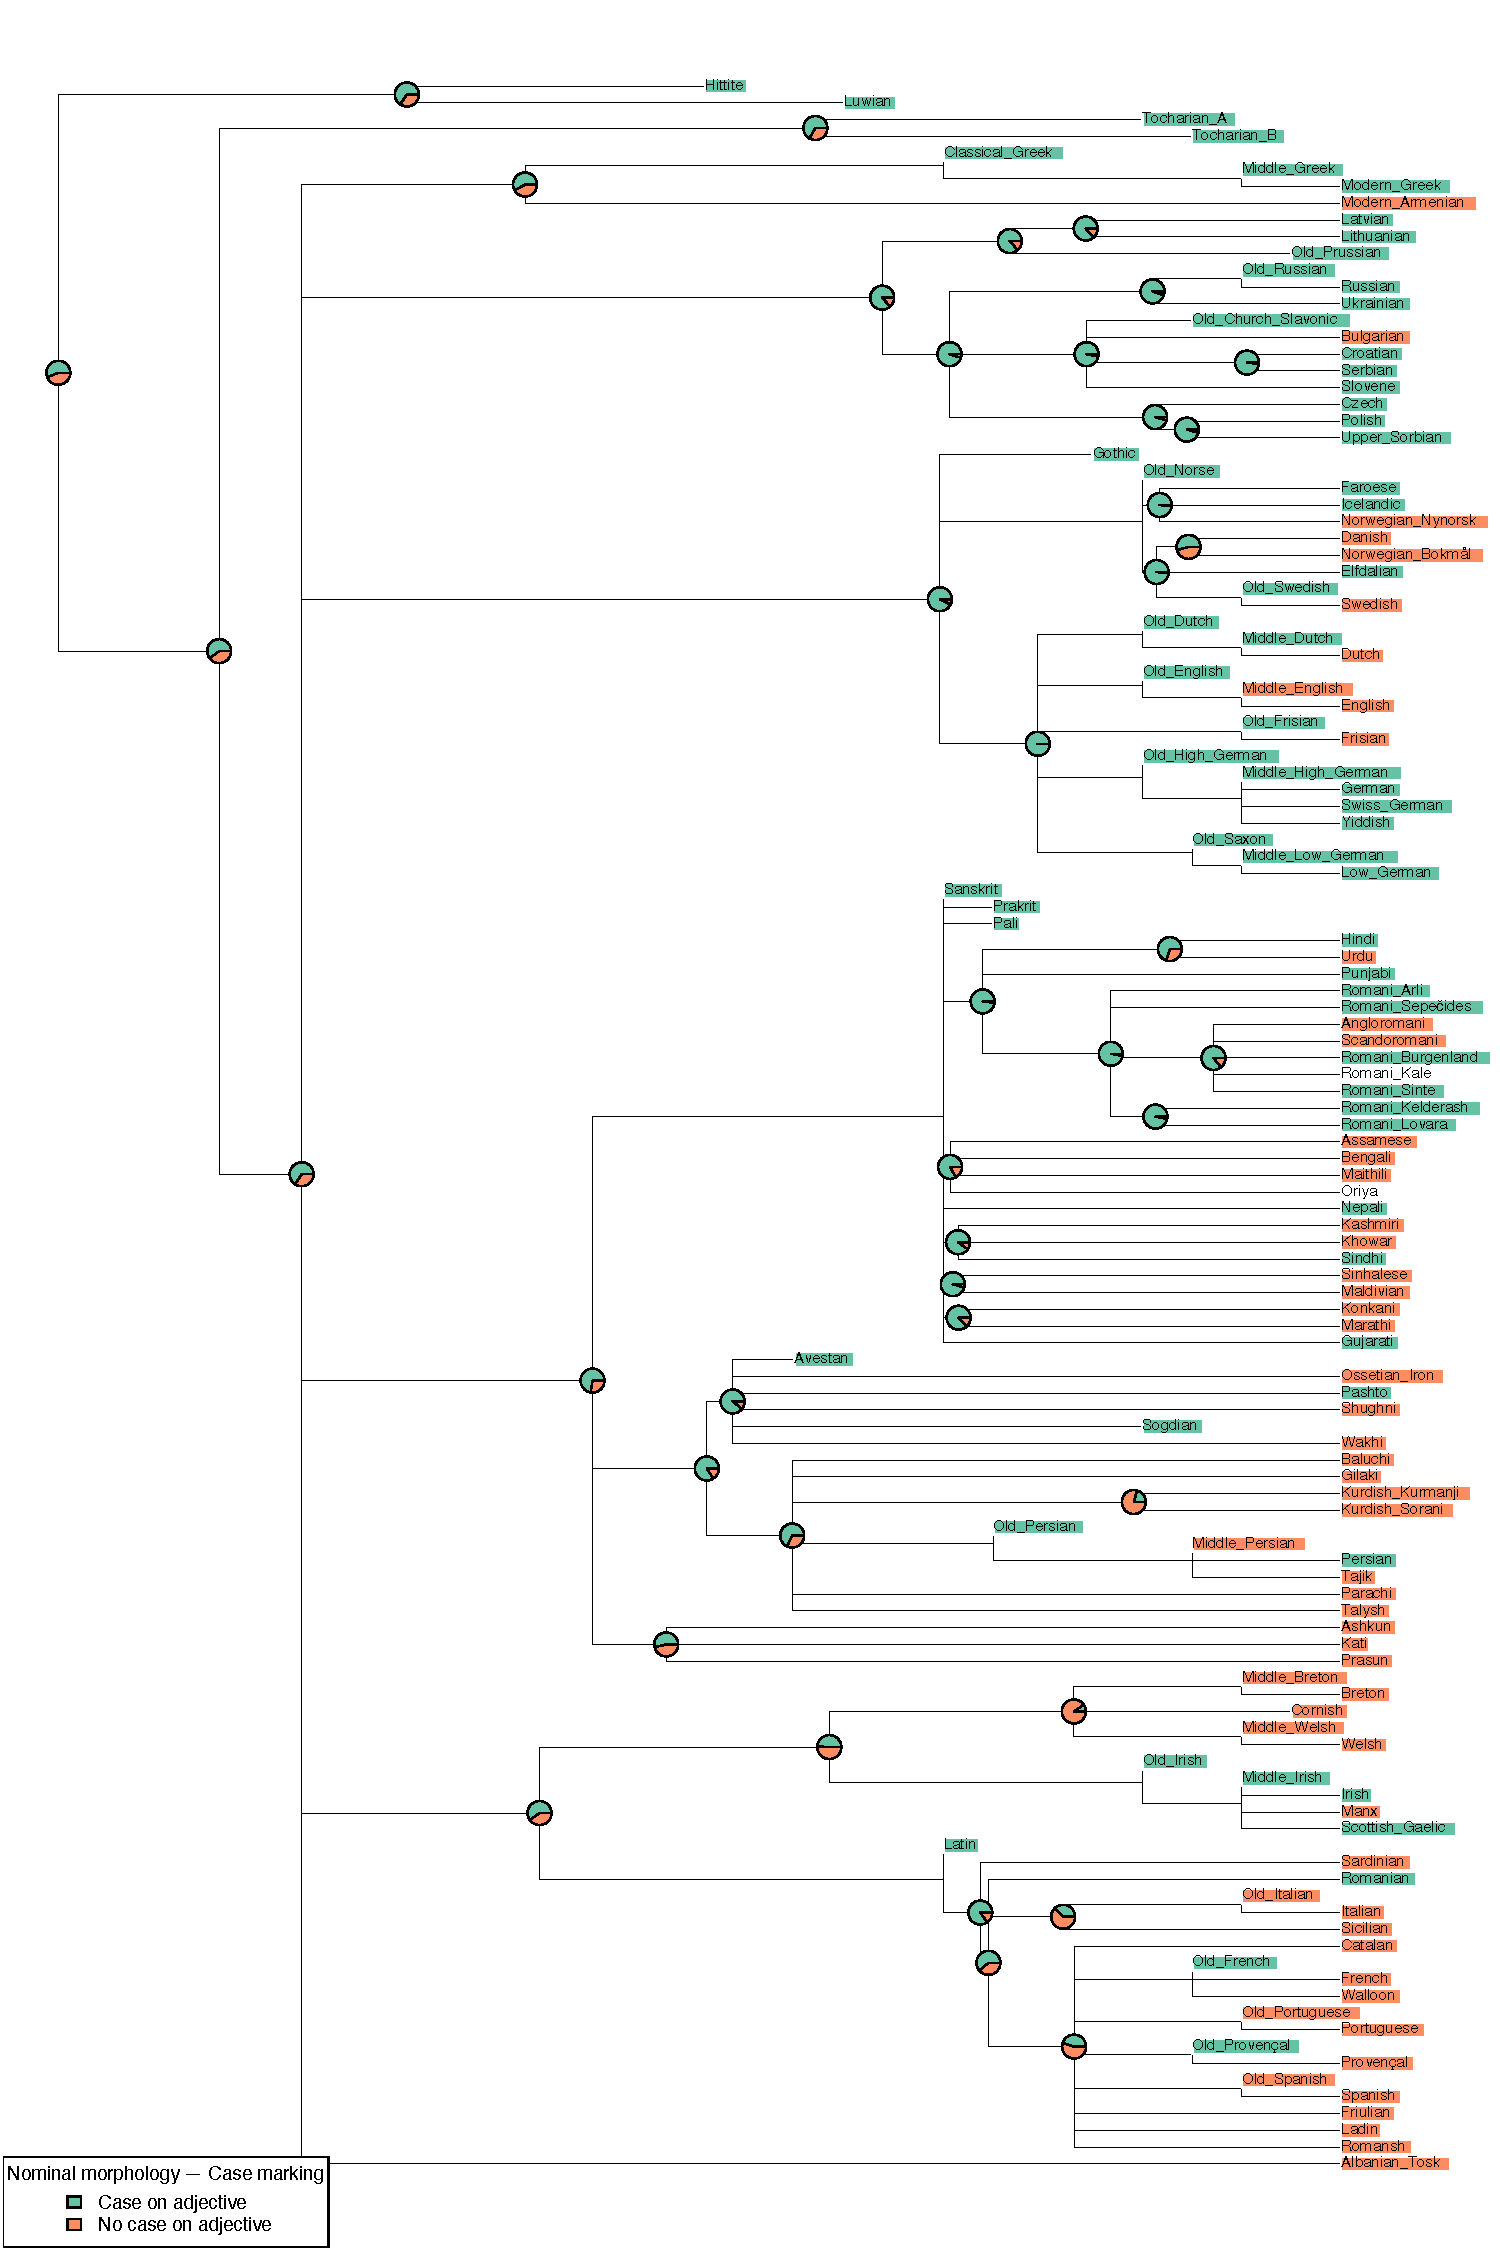
\includegraphics[width=.9\linewidth]{supp-graphics/NominalmorphologyCasemarkingCASEADJ.pdf}

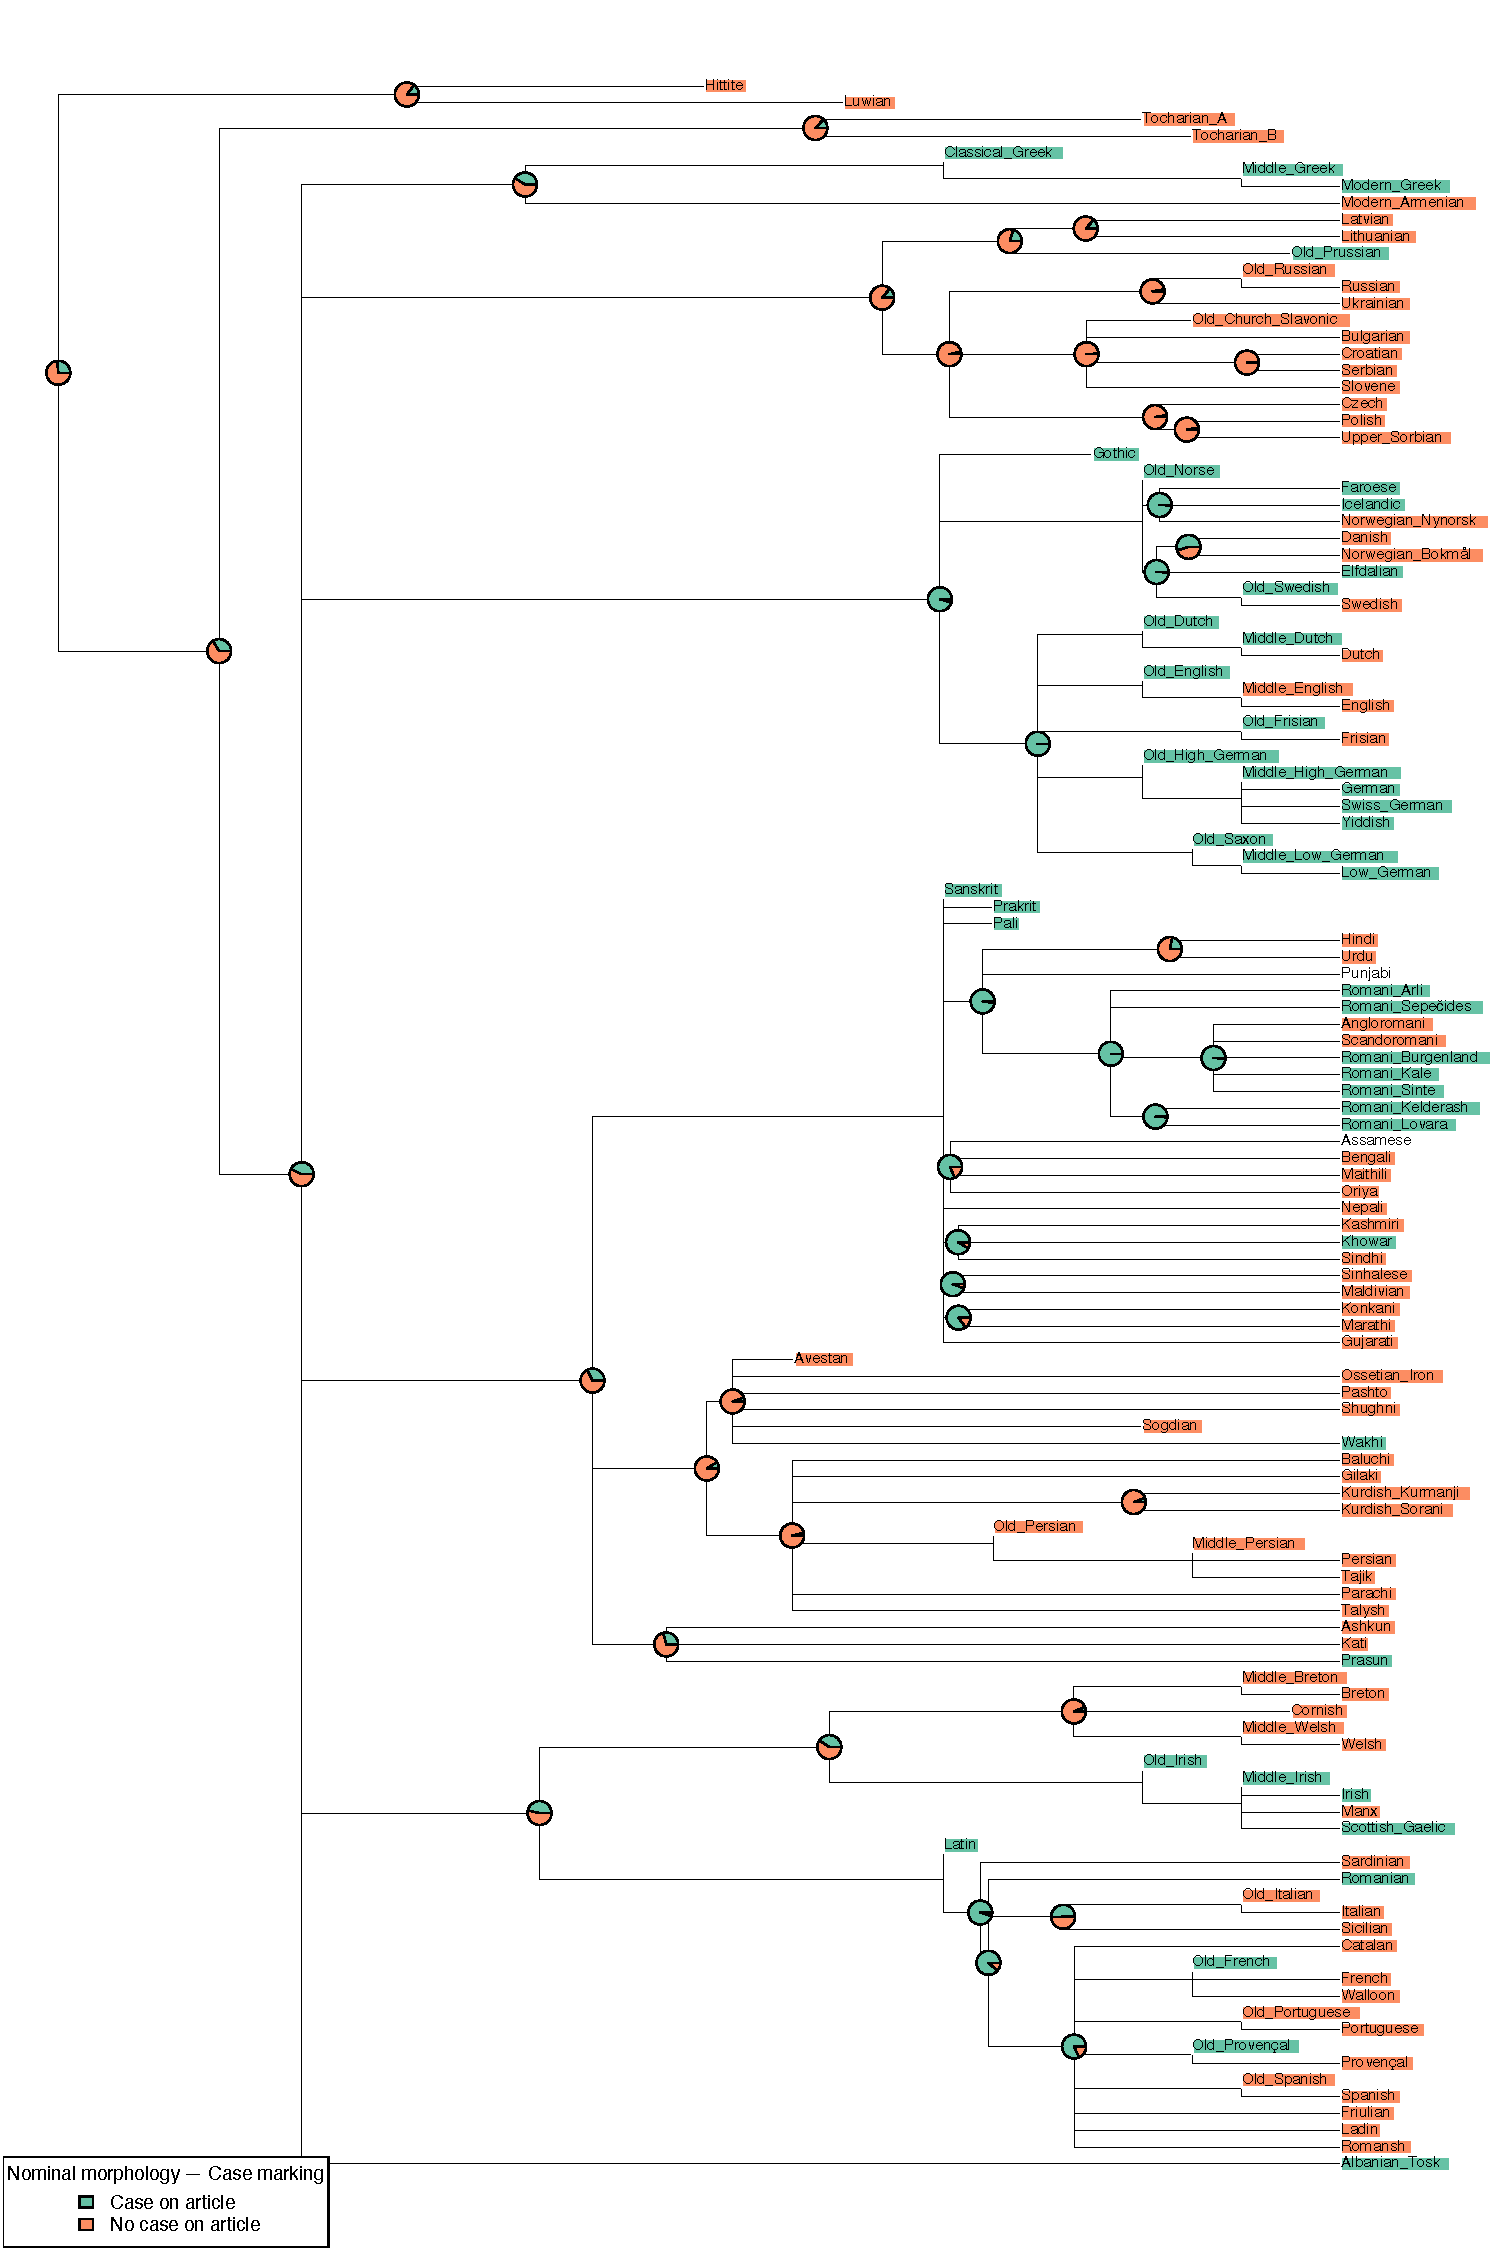
\includegraphics[width=.9\linewidth]{supp-graphics/NominalmorphologyCasemarkingCASEART.pdf}

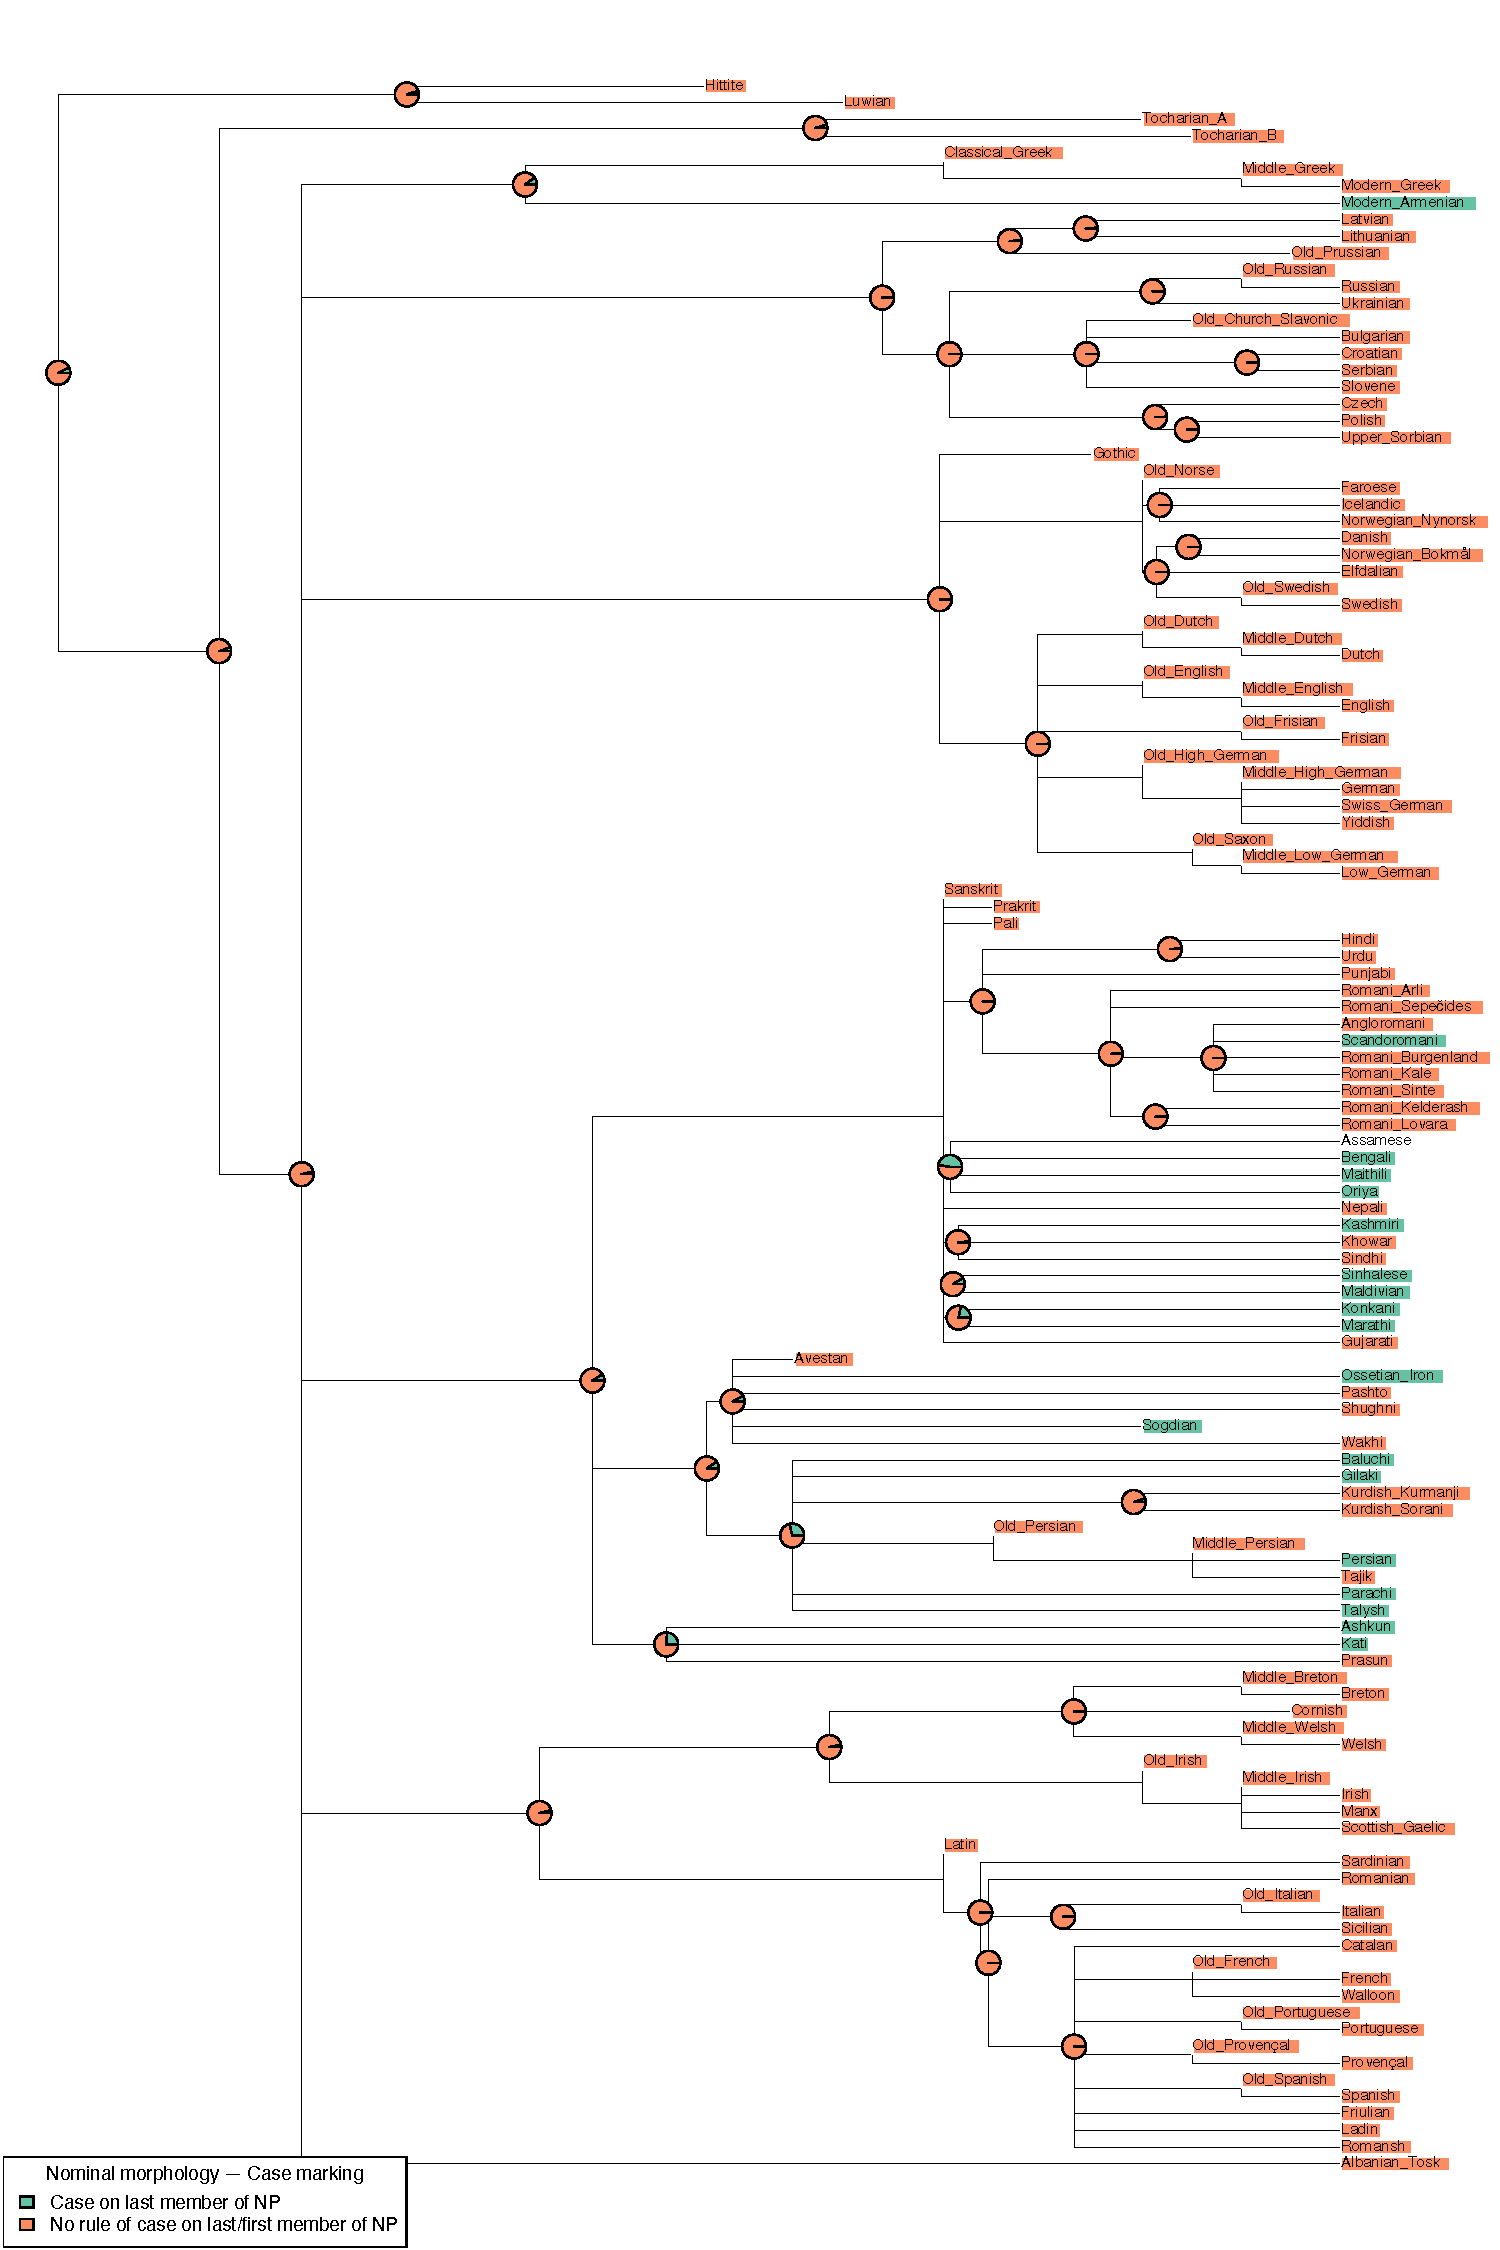
\includegraphics[width=.9\linewidth]{supp-graphics/NominalmorphologyCasemarkingCASEFIRSTNominalmorphologyCasemarkingCASELAST.pdf}

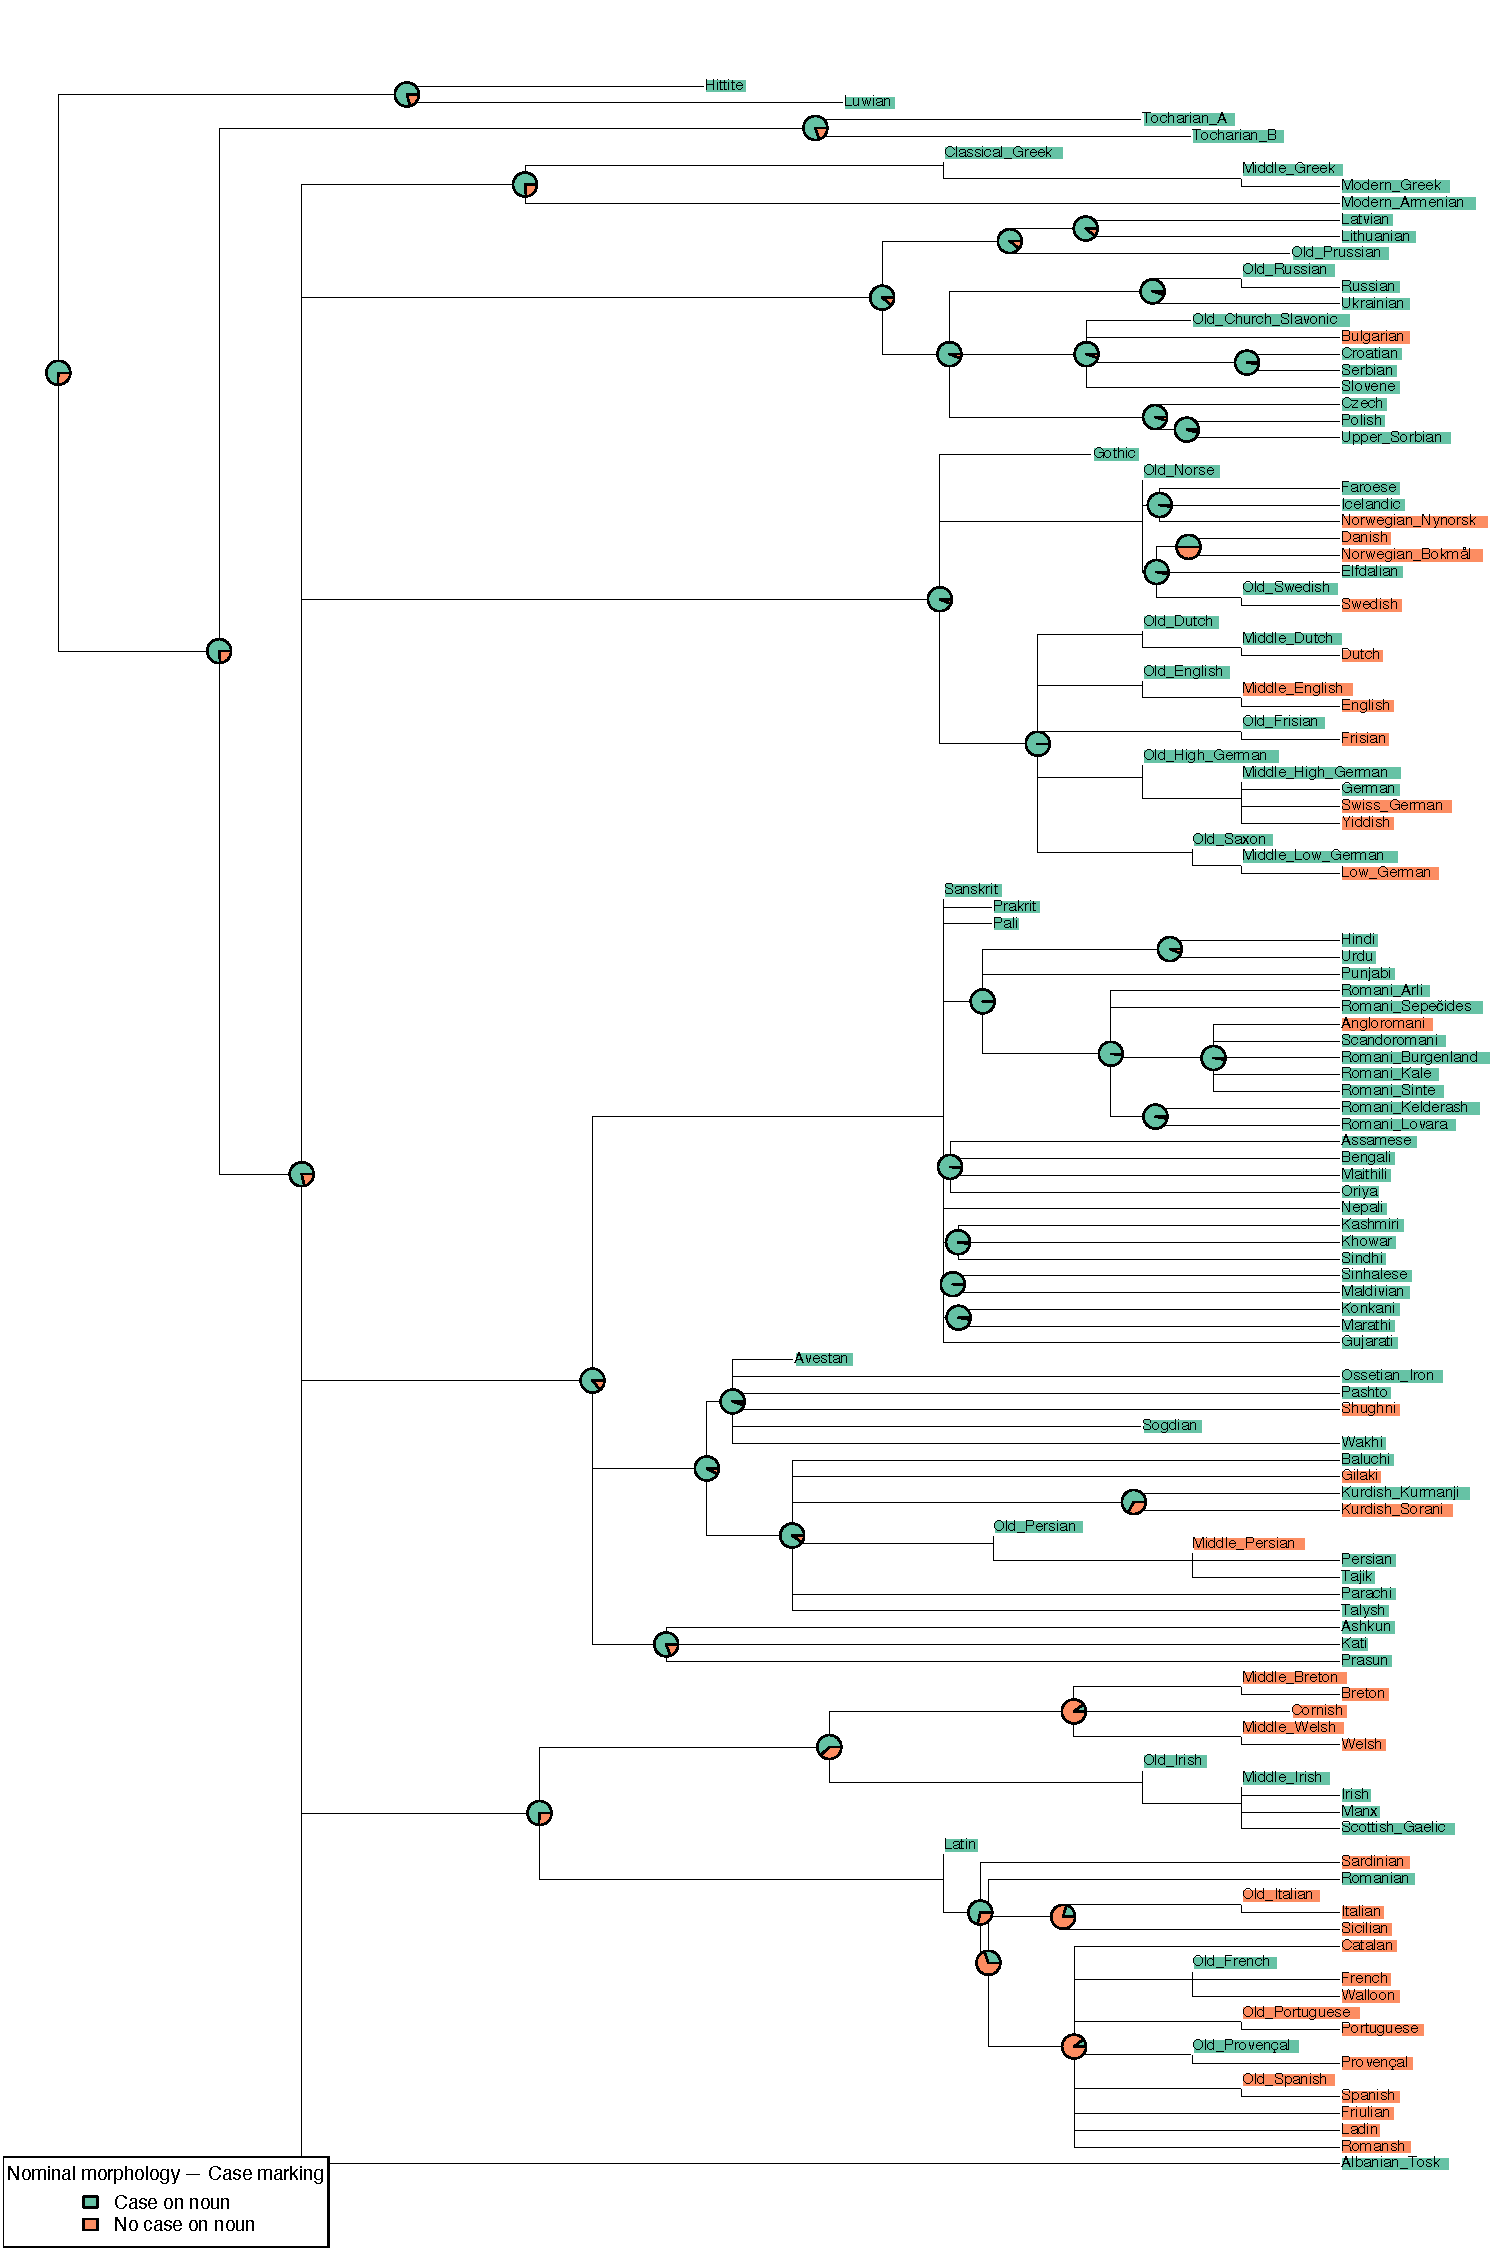
\includegraphics[width=.9\linewidth]{supp-graphics/NominalmorphologyCasemarkingCASEN.pdf}

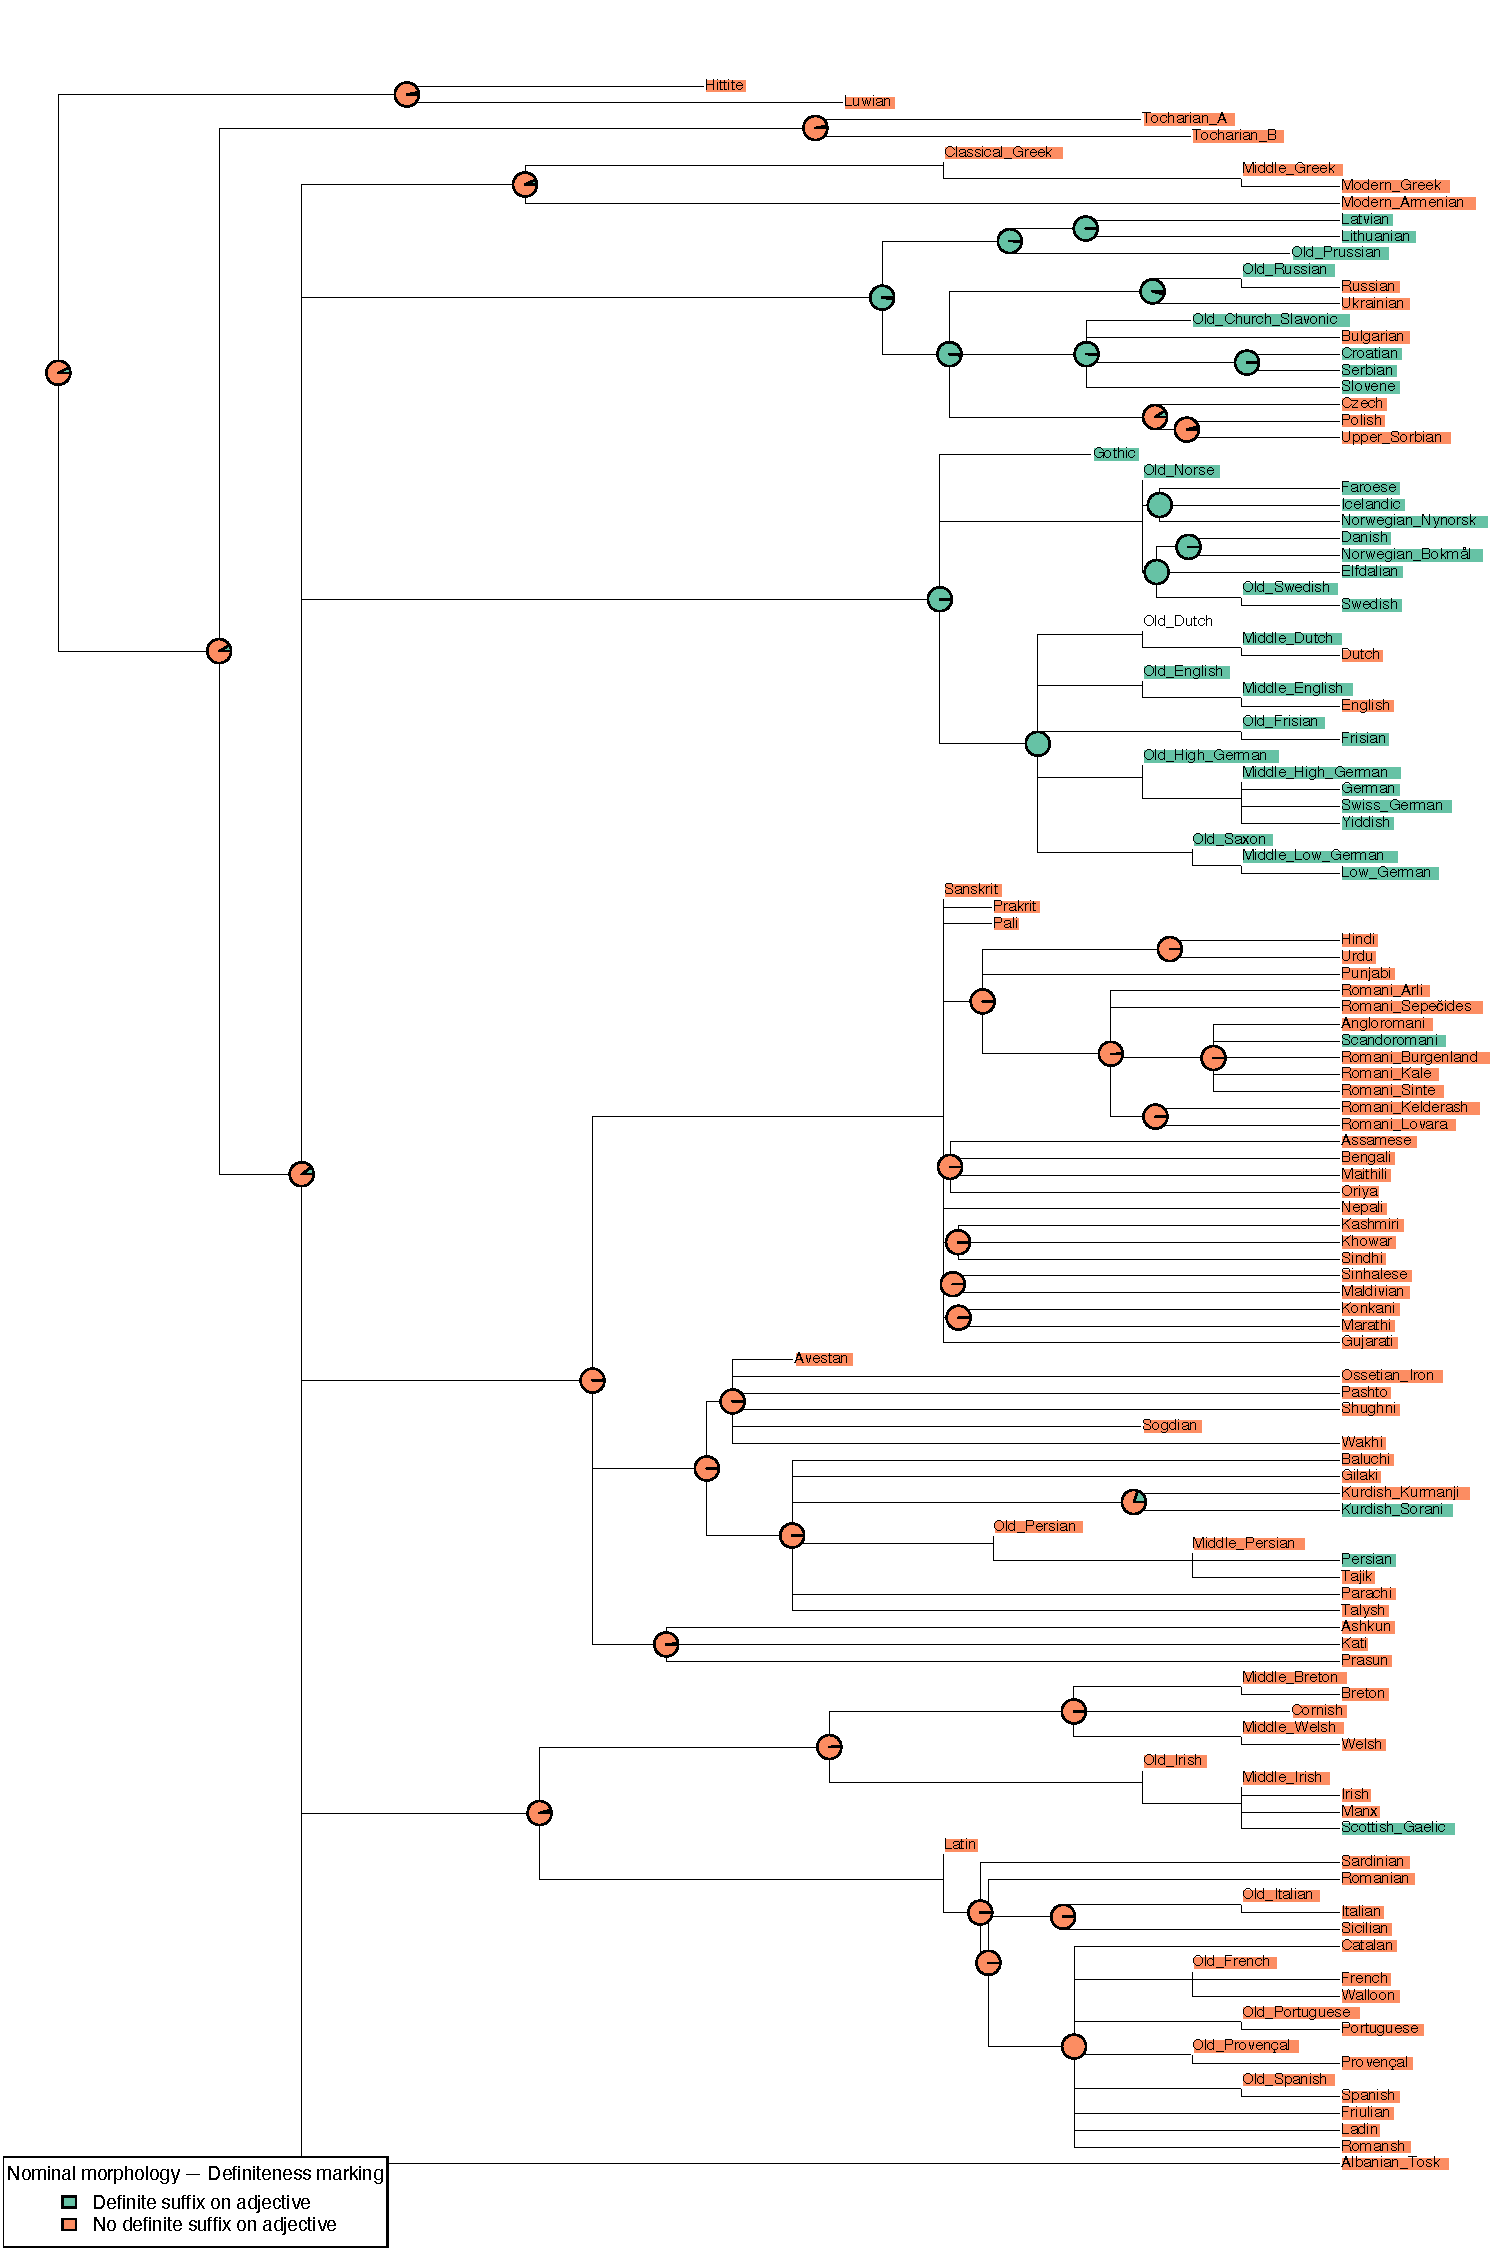
\includegraphics[width=.9\linewidth]{supp-graphics/NominalmorphologyDefinitenessmarkingADJDEF.pdf}

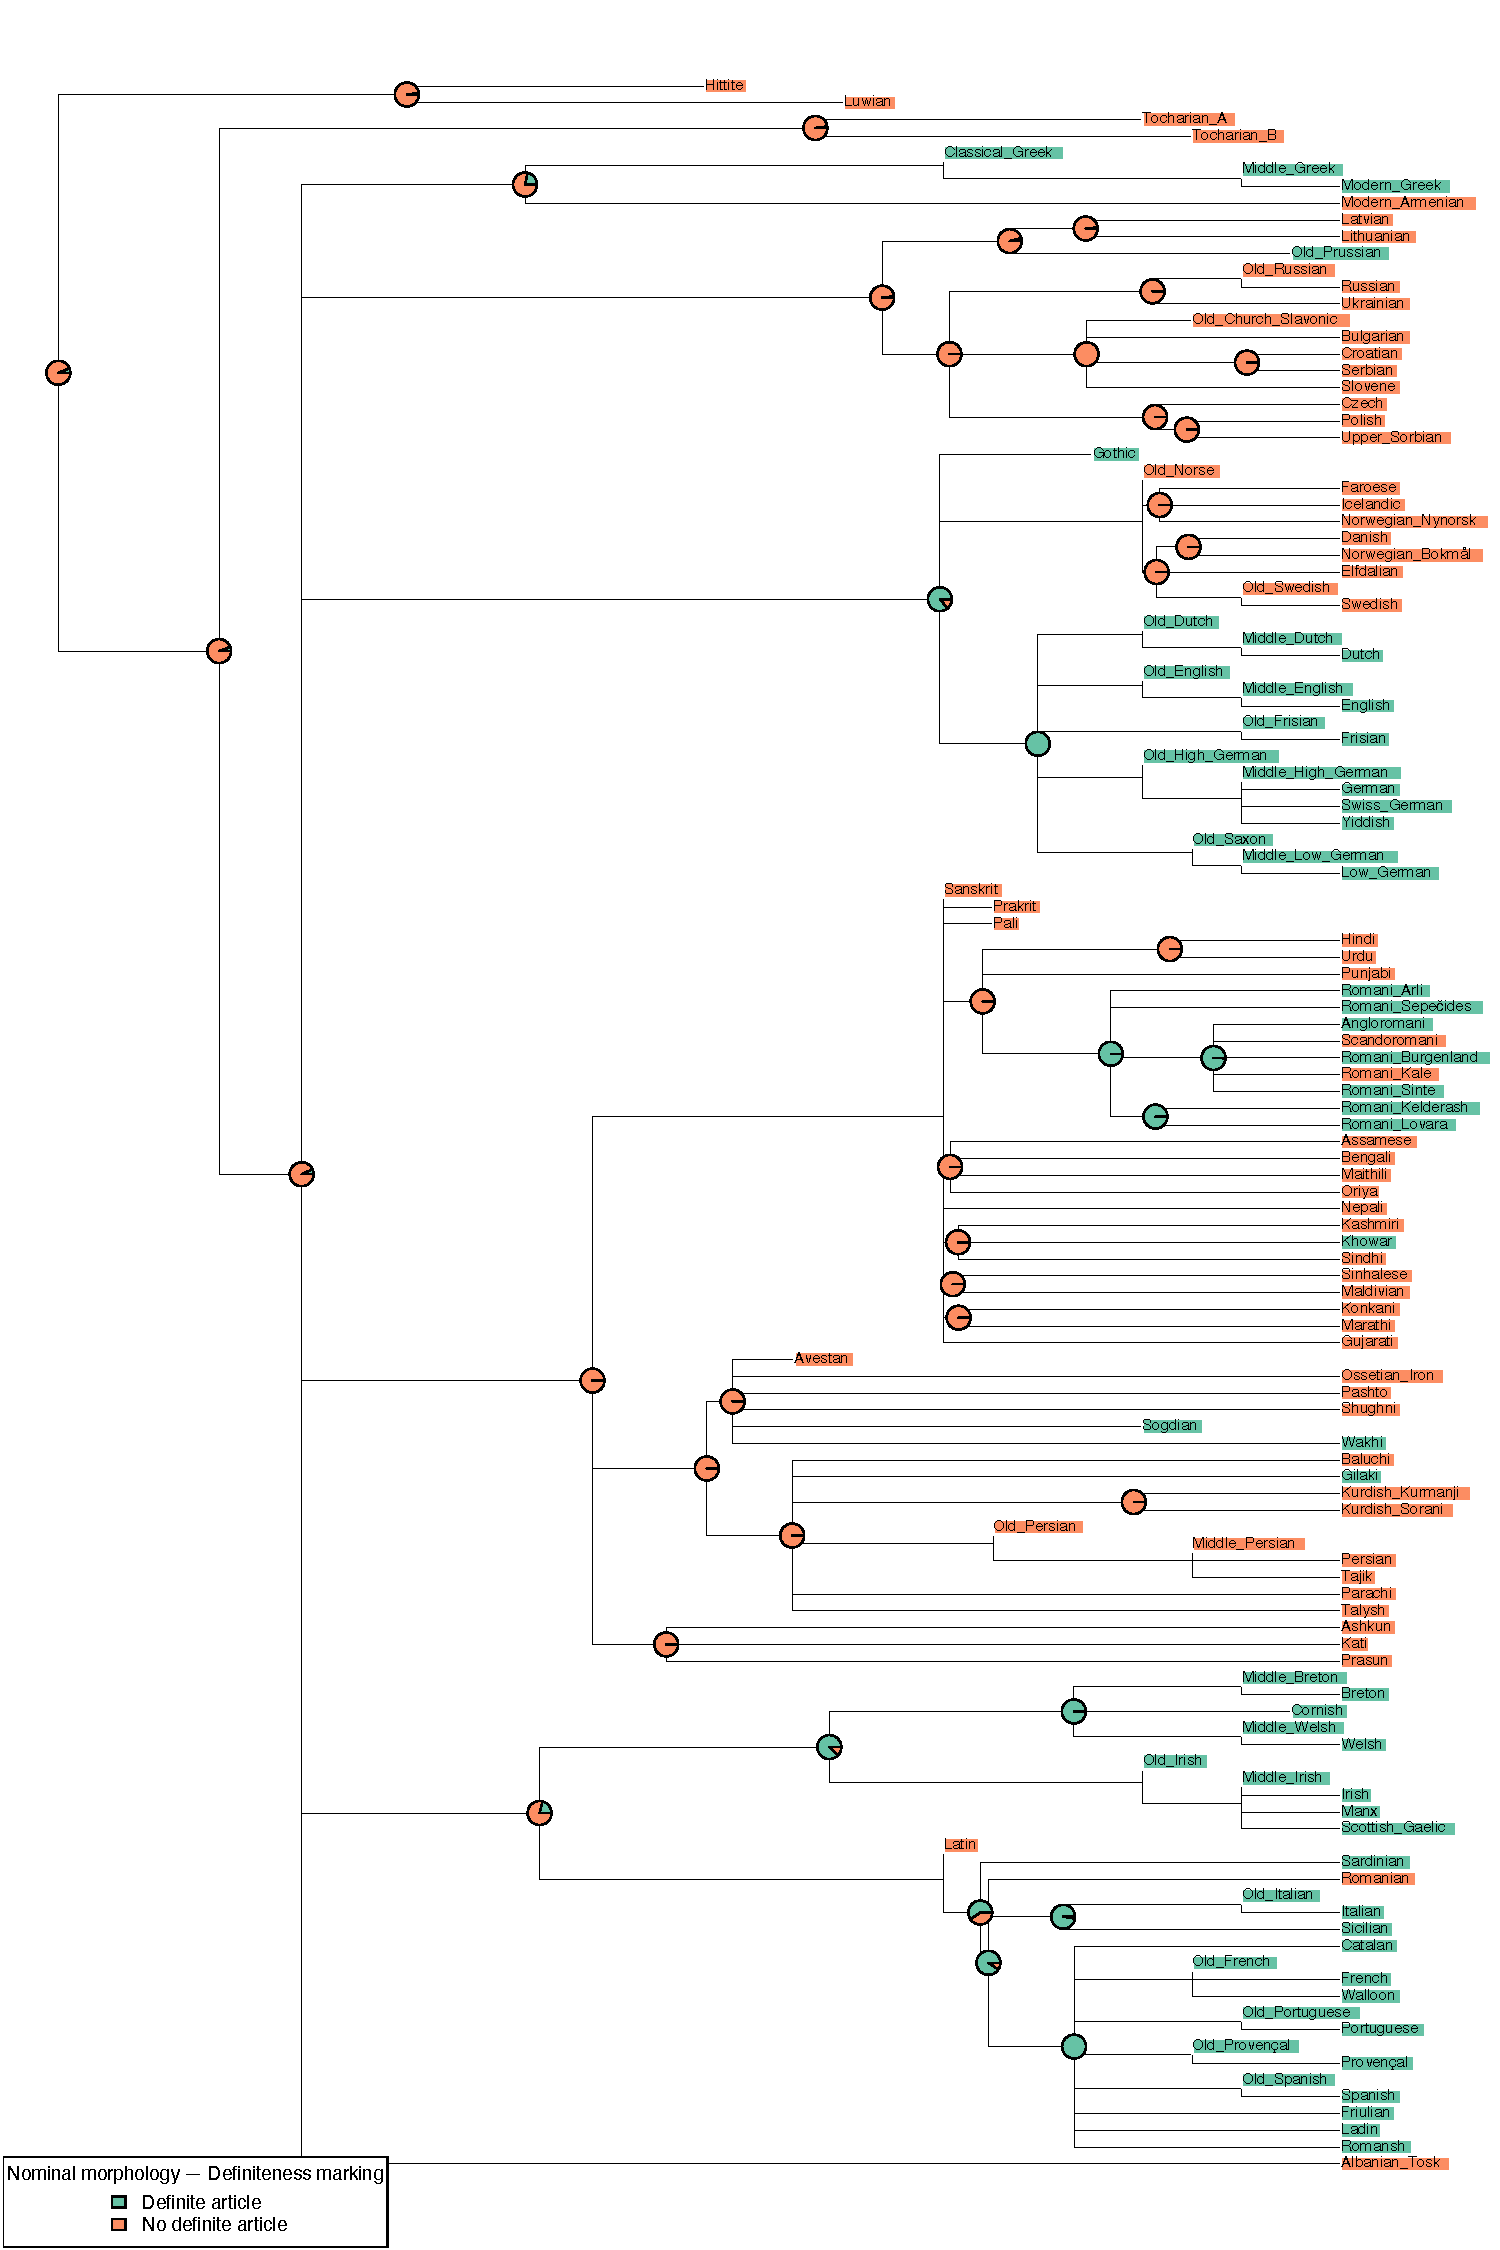
\includegraphics[width=.9\linewidth]{supp-graphics/NominalmorphologyDefinitenessmarkingDEFART.pdf}

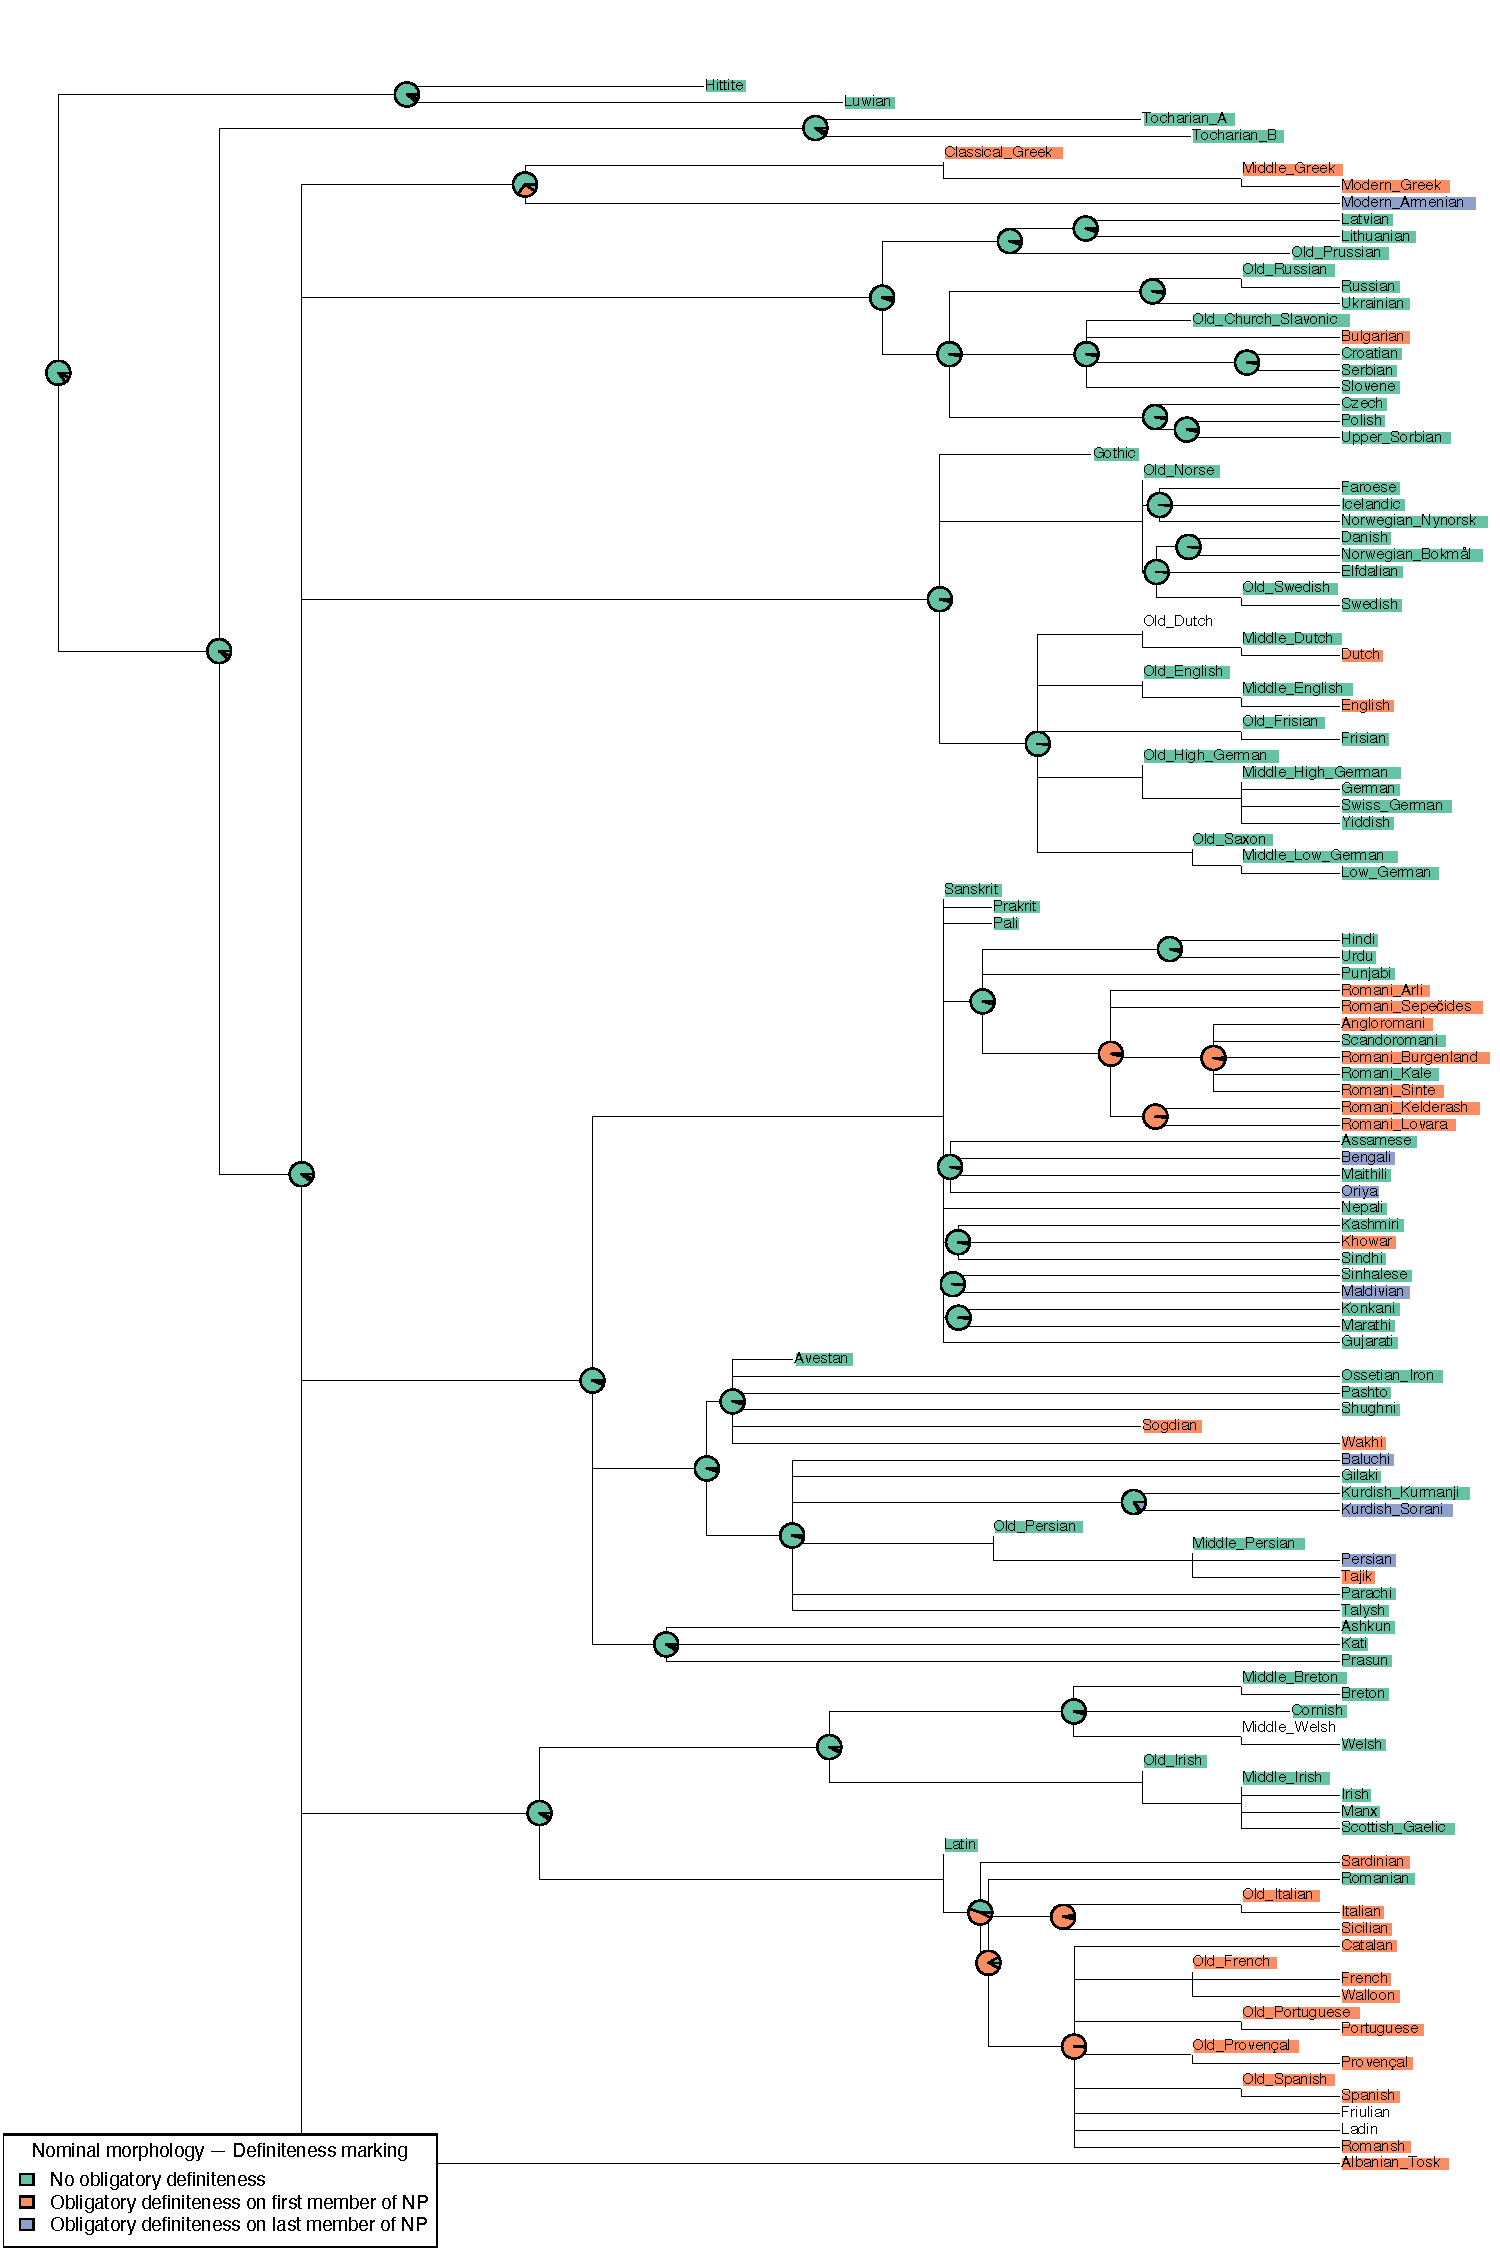
\includegraphics[width=.9\linewidth]{supp-graphics/NominalmorphologyDefinitenessmarkingDEFFIRSTNominalmorphologyDefinitenessmarkingDEFLAST.pdf}

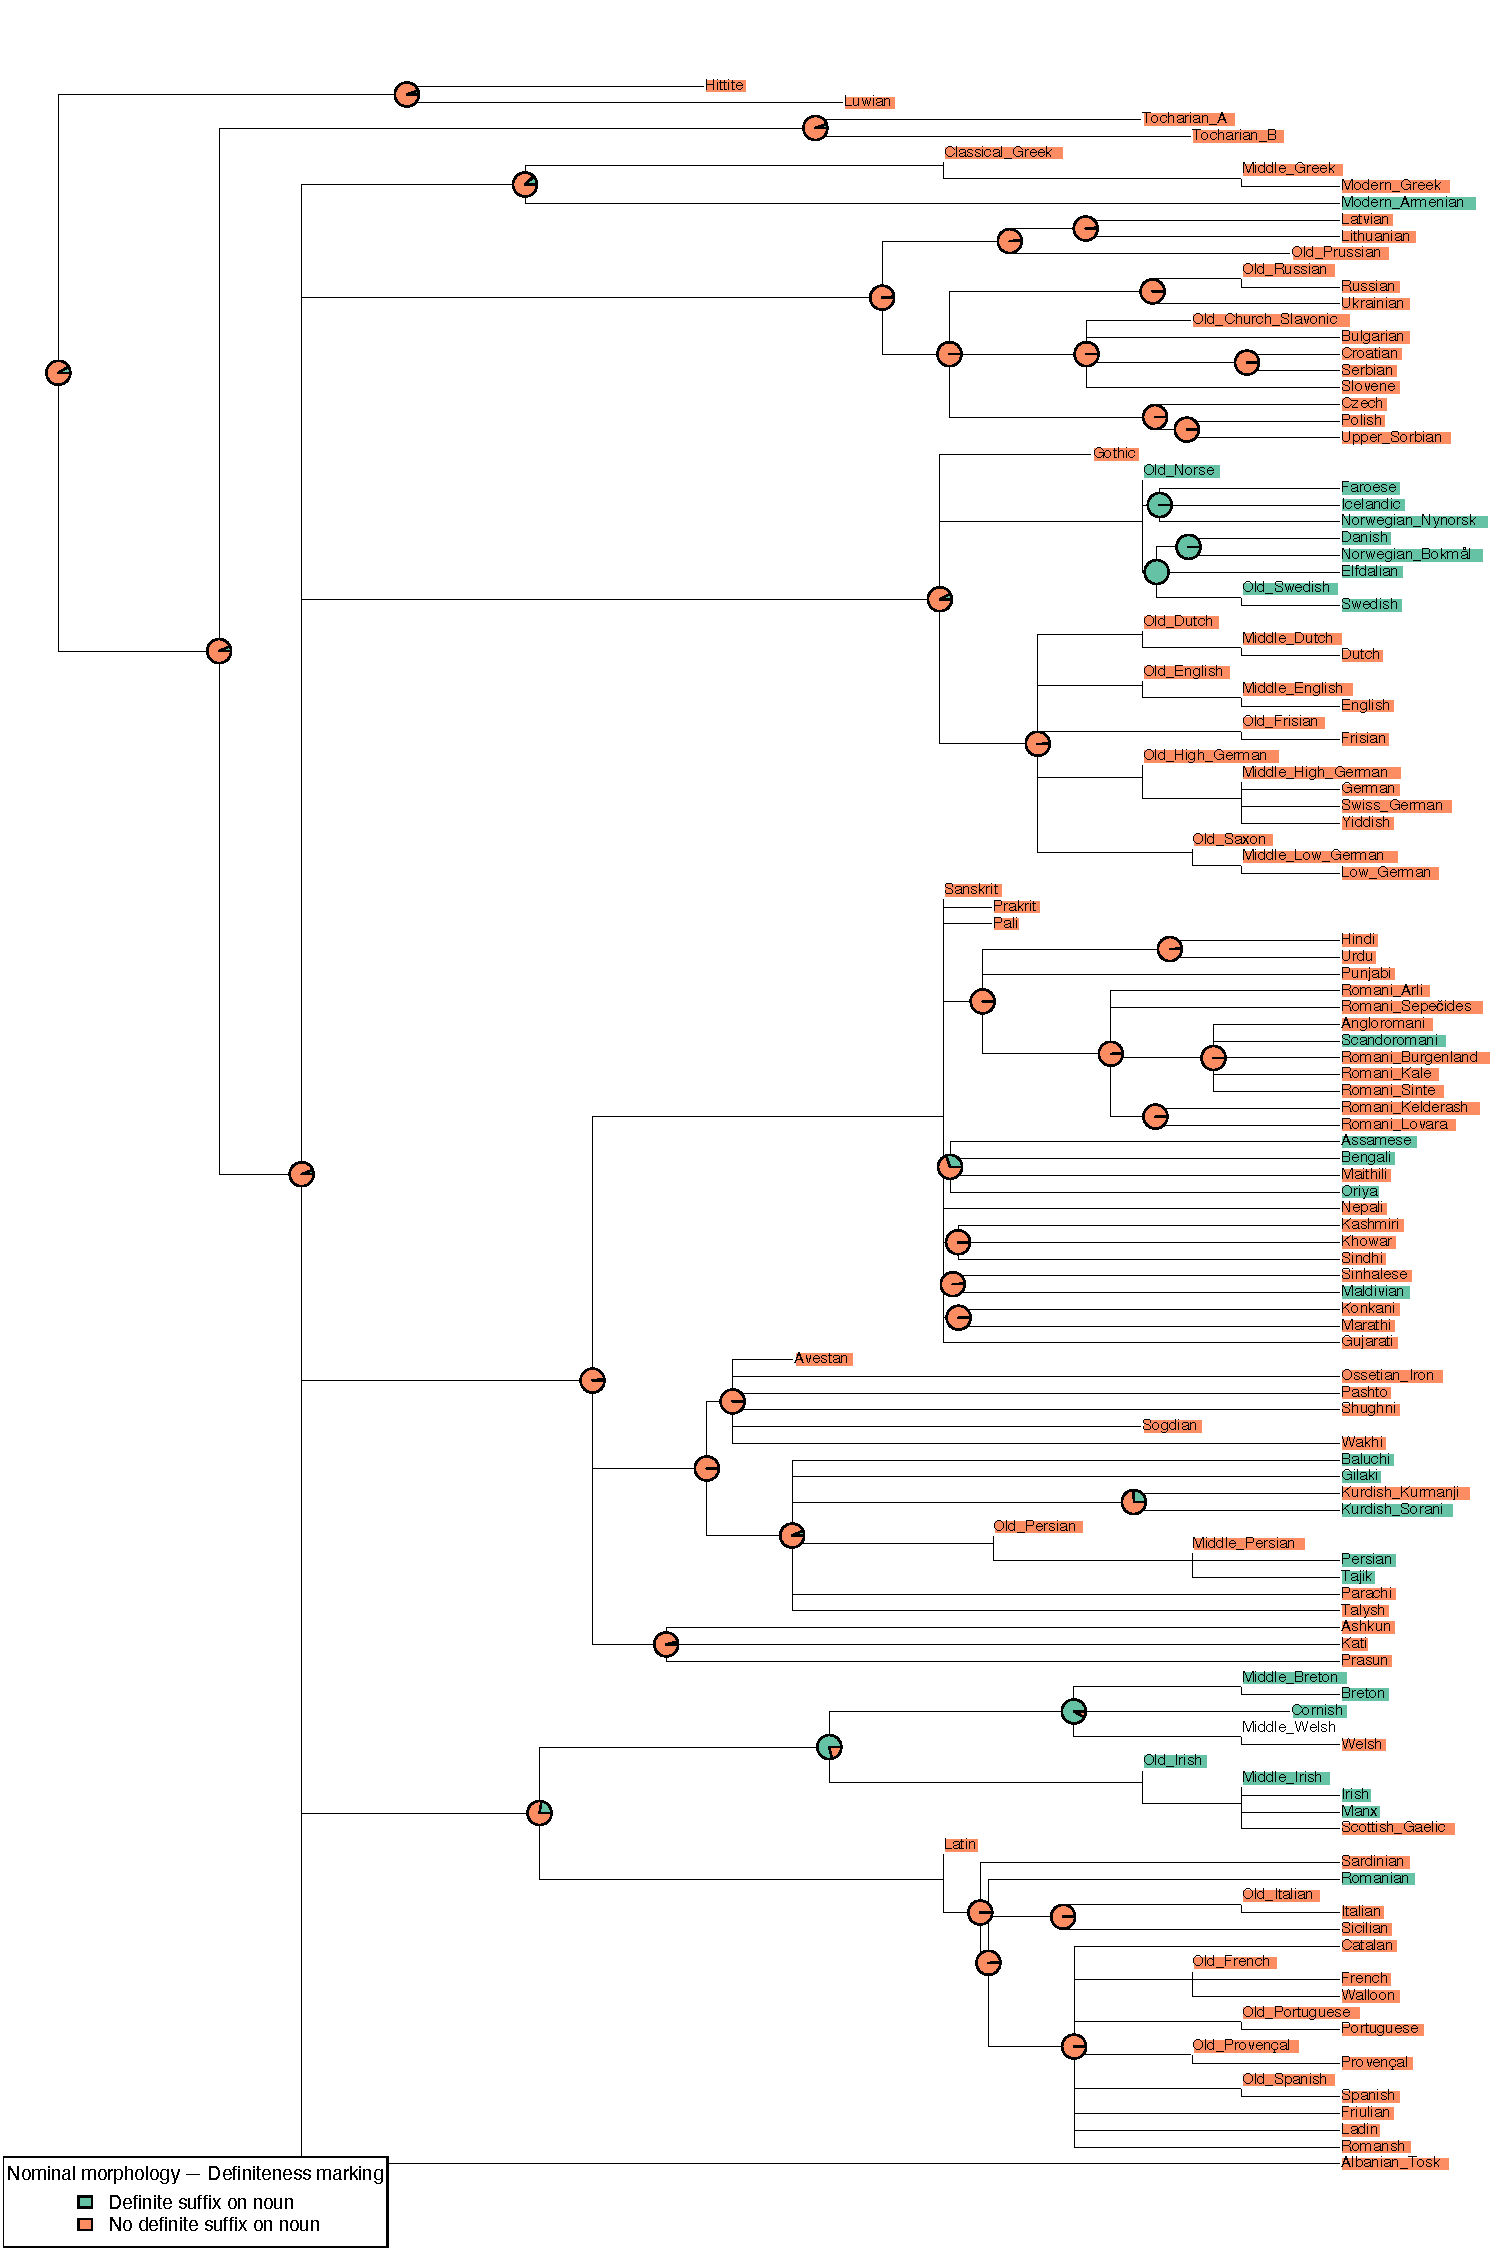
\includegraphics[width=.9\linewidth]{supp-graphics/NominalmorphologyDefinitenessmarkingNDEF.pdf}

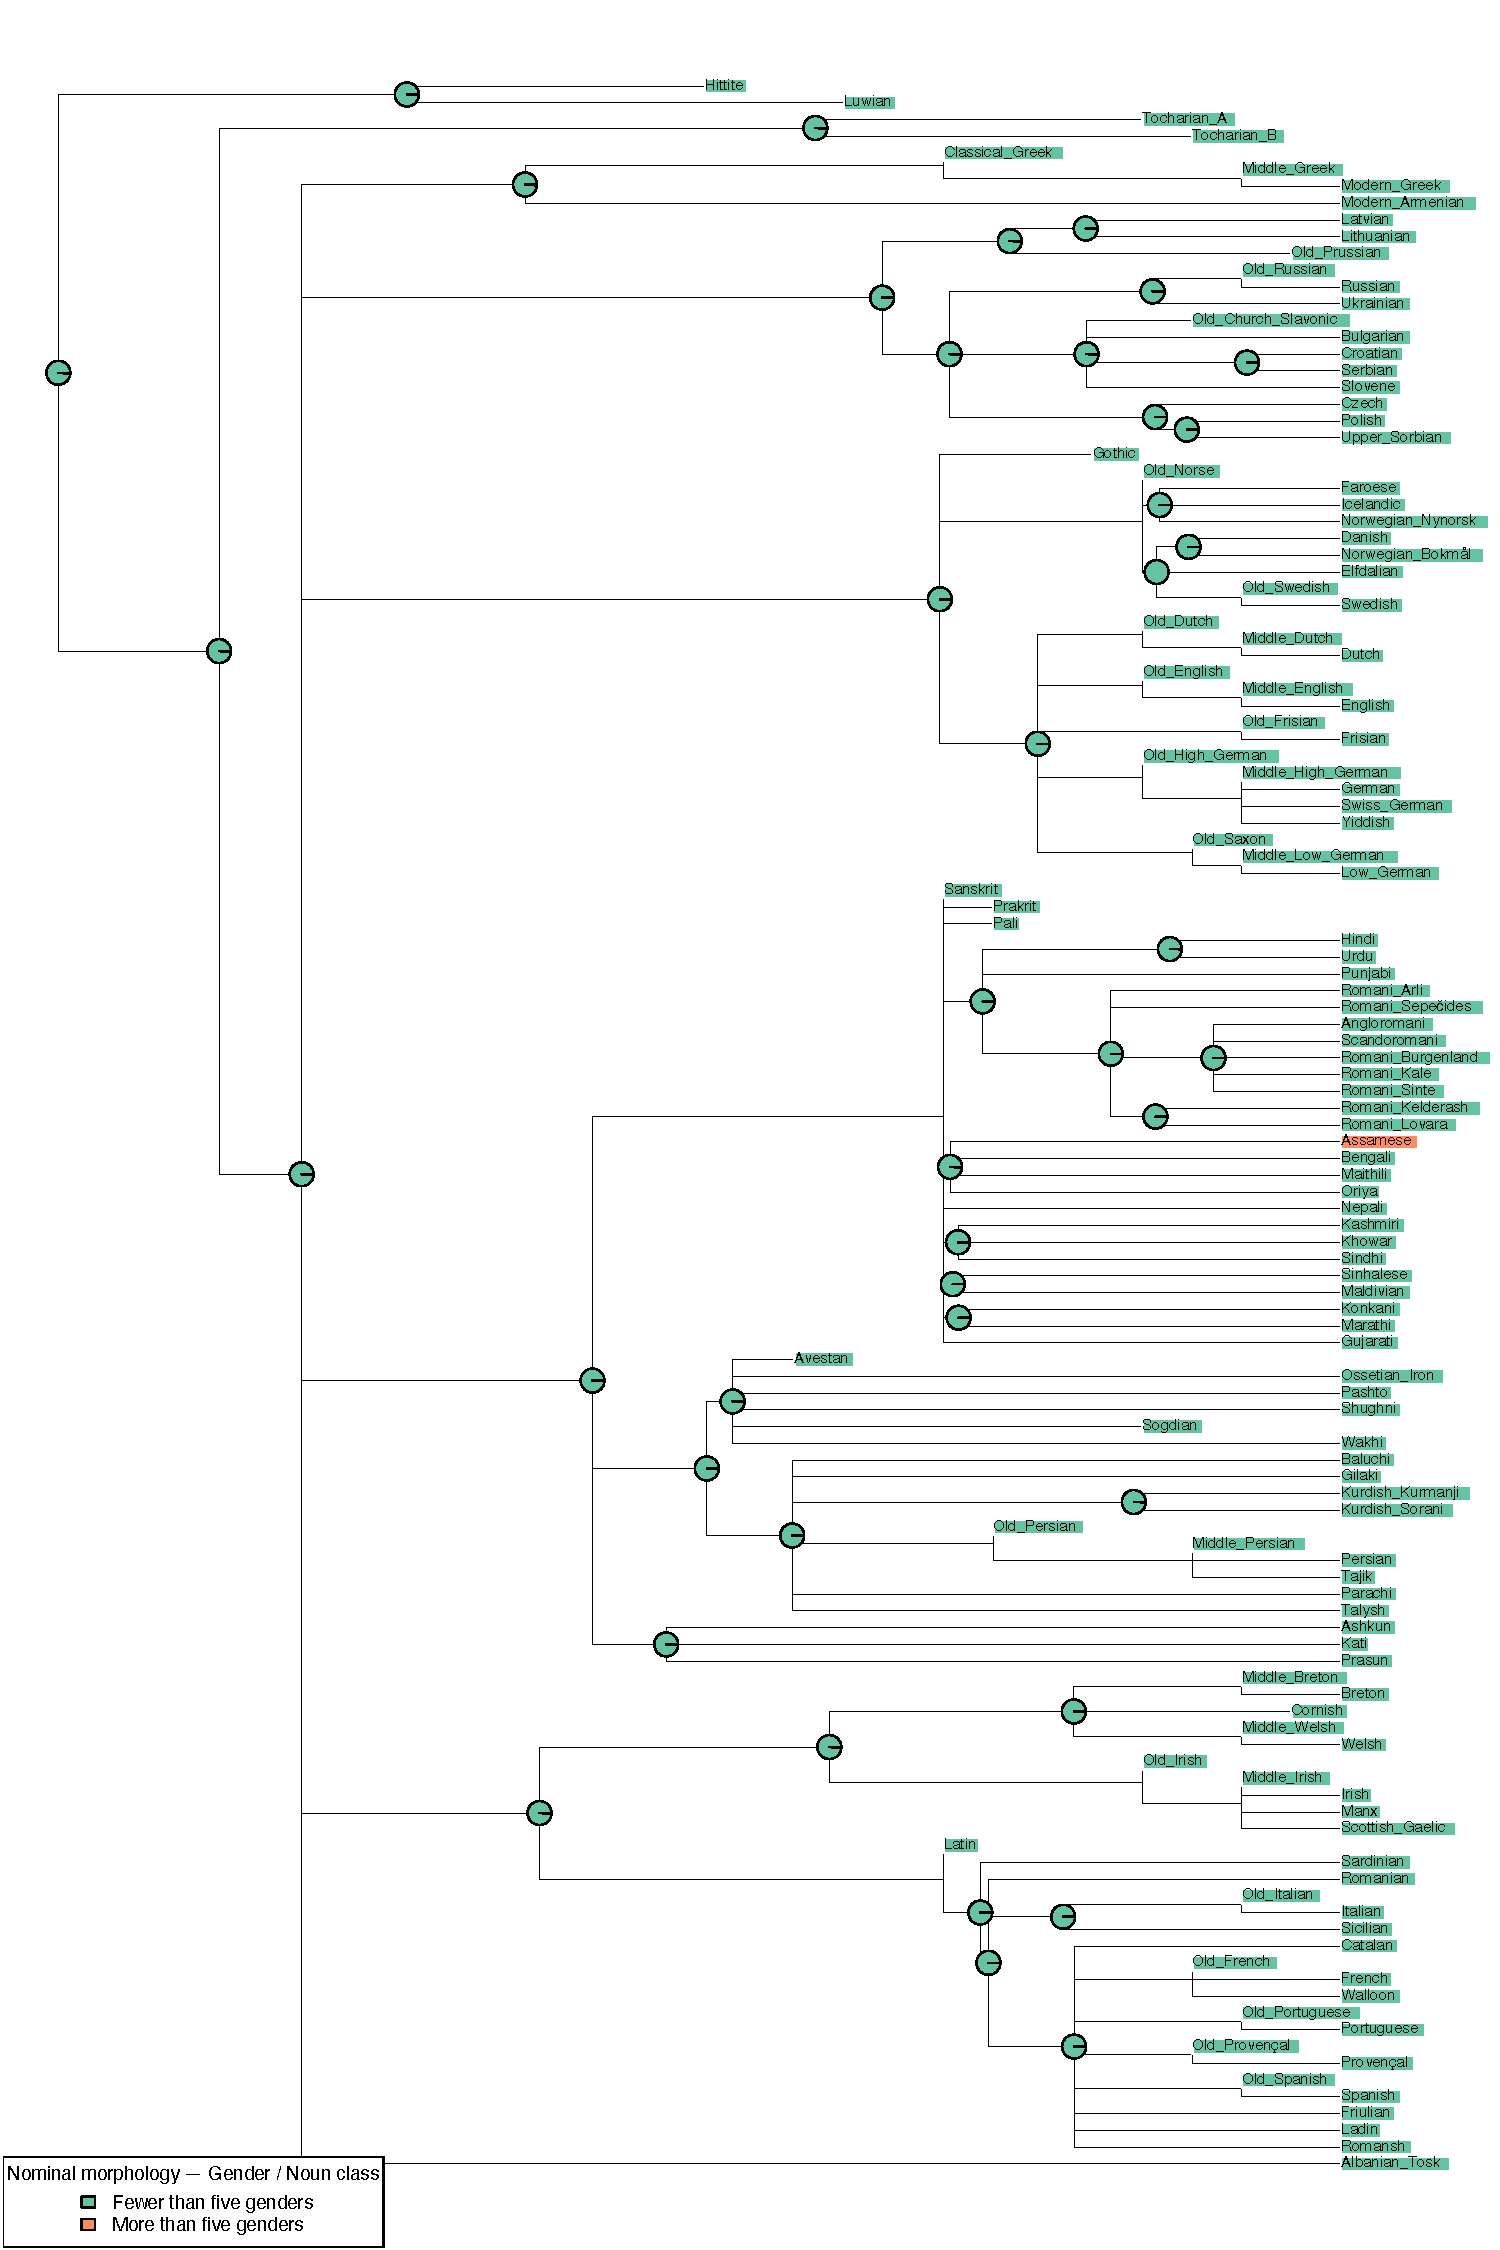
\includegraphics[width=.9\linewidth]{supp-graphics/NominalmorphologyGenderNounclass5GENDER.pdf}

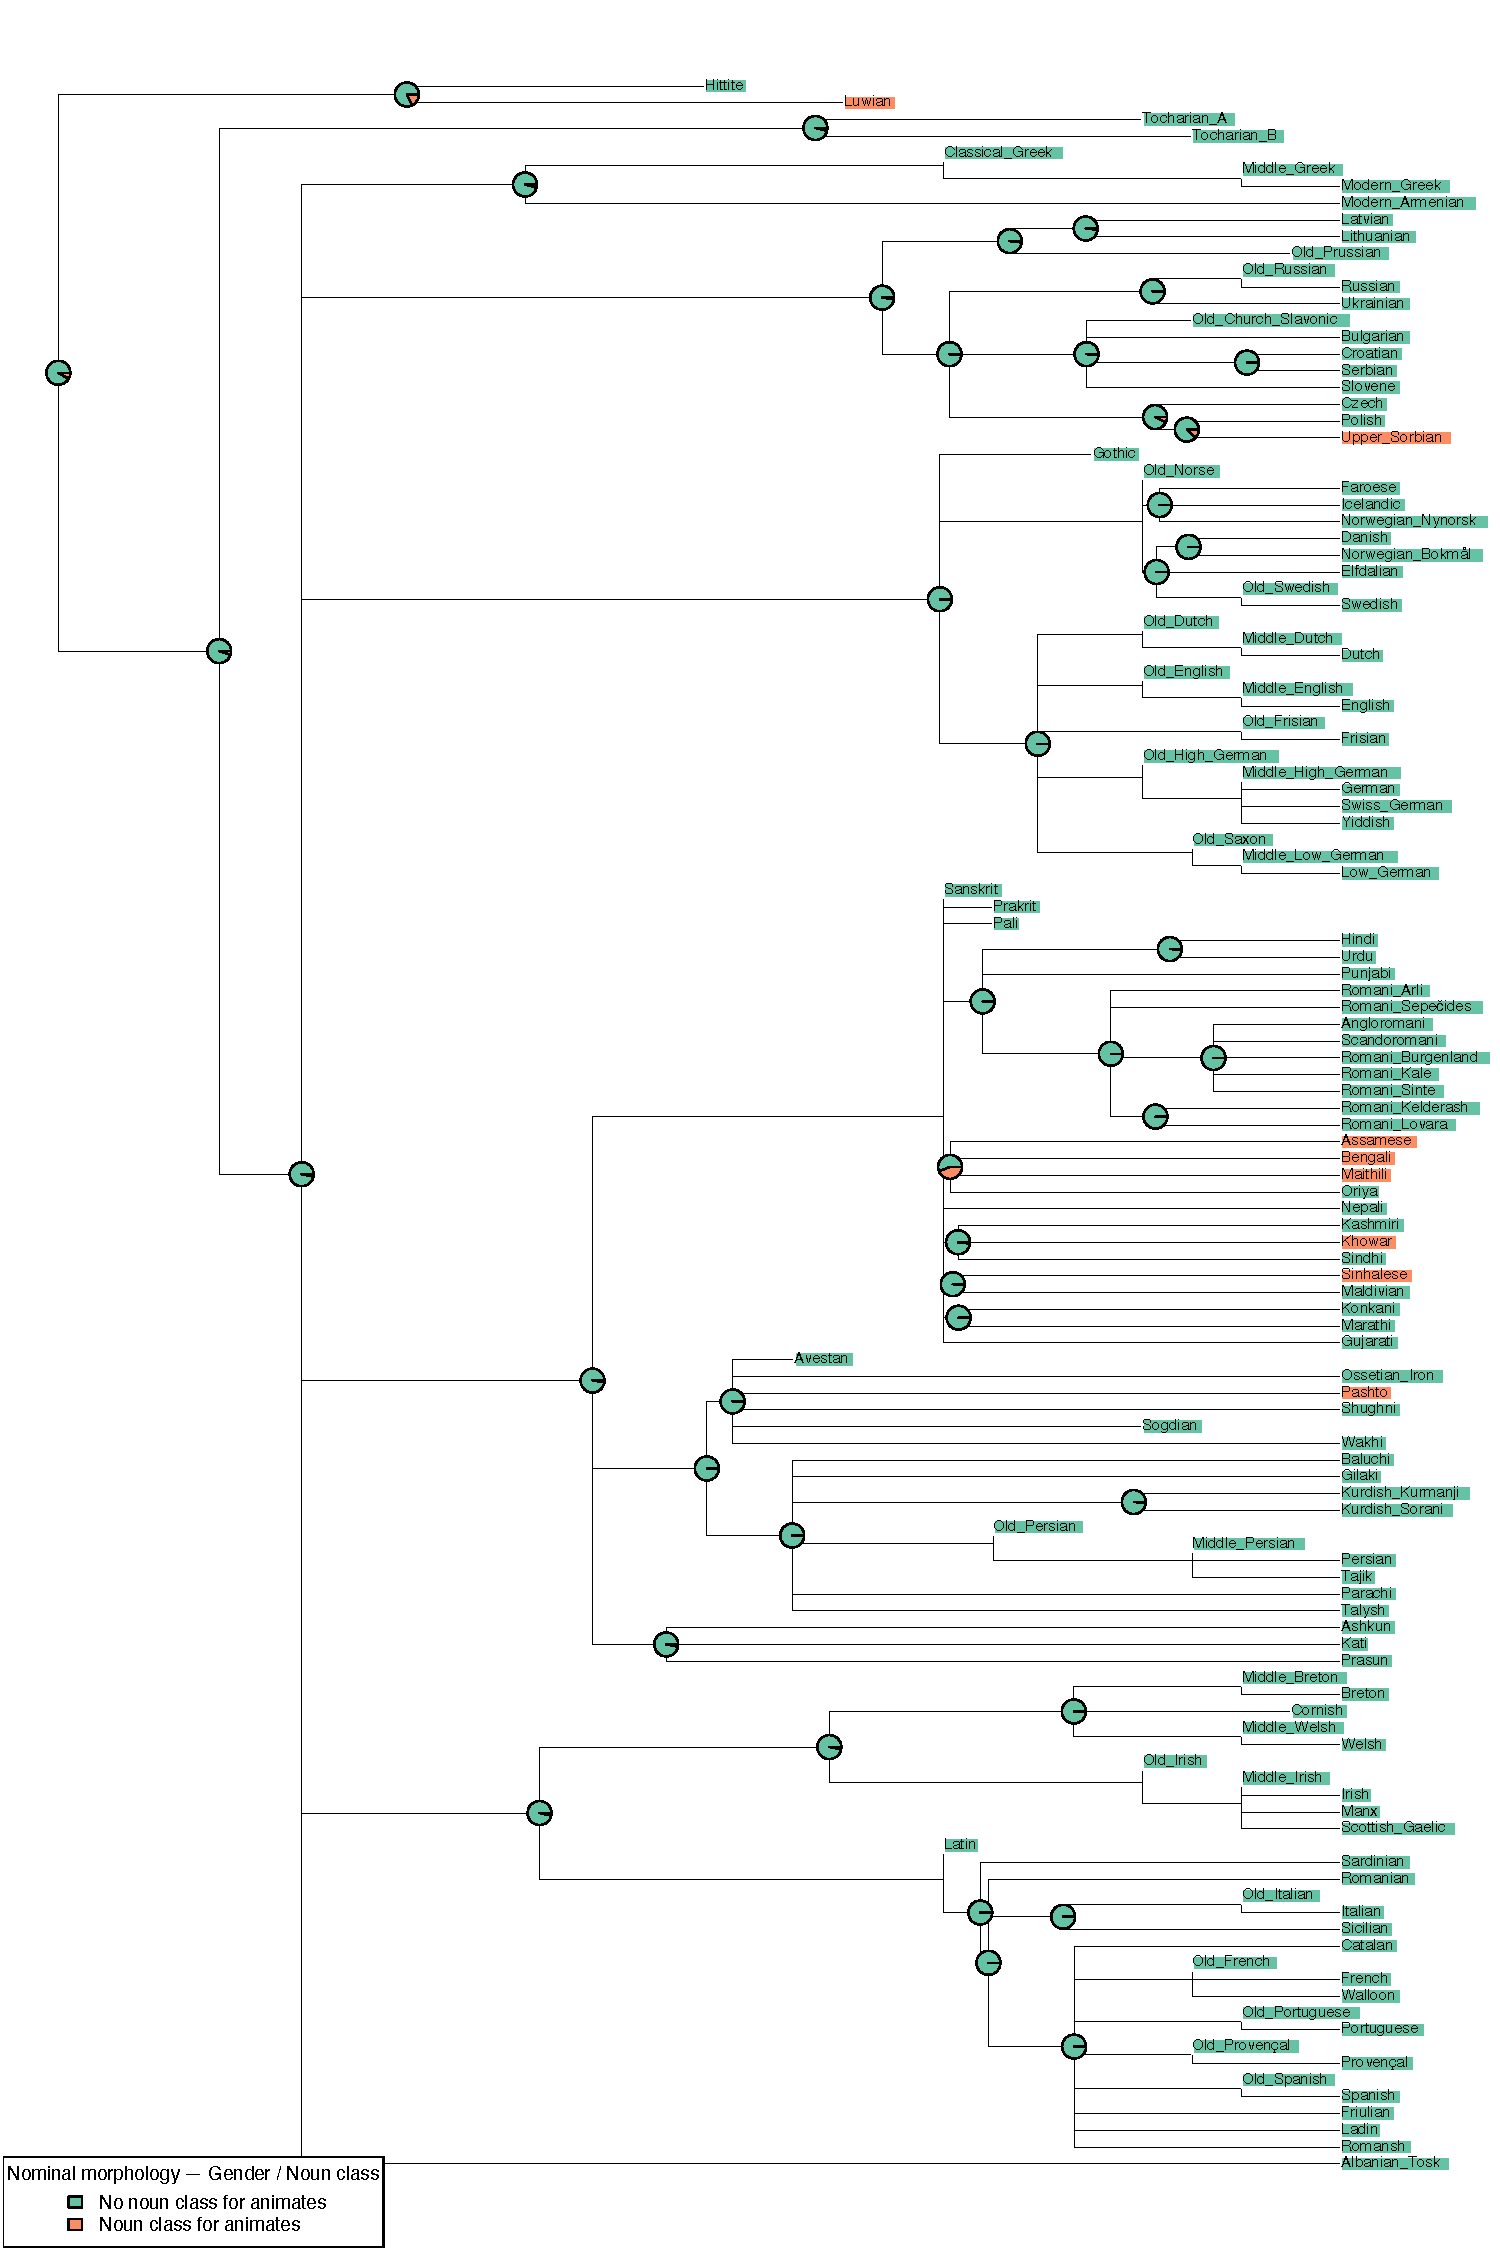
\includegraphics[width=.9\linewidth]{supp-graphics/NominalmorphologyGenderNounclassANIM.pdf}

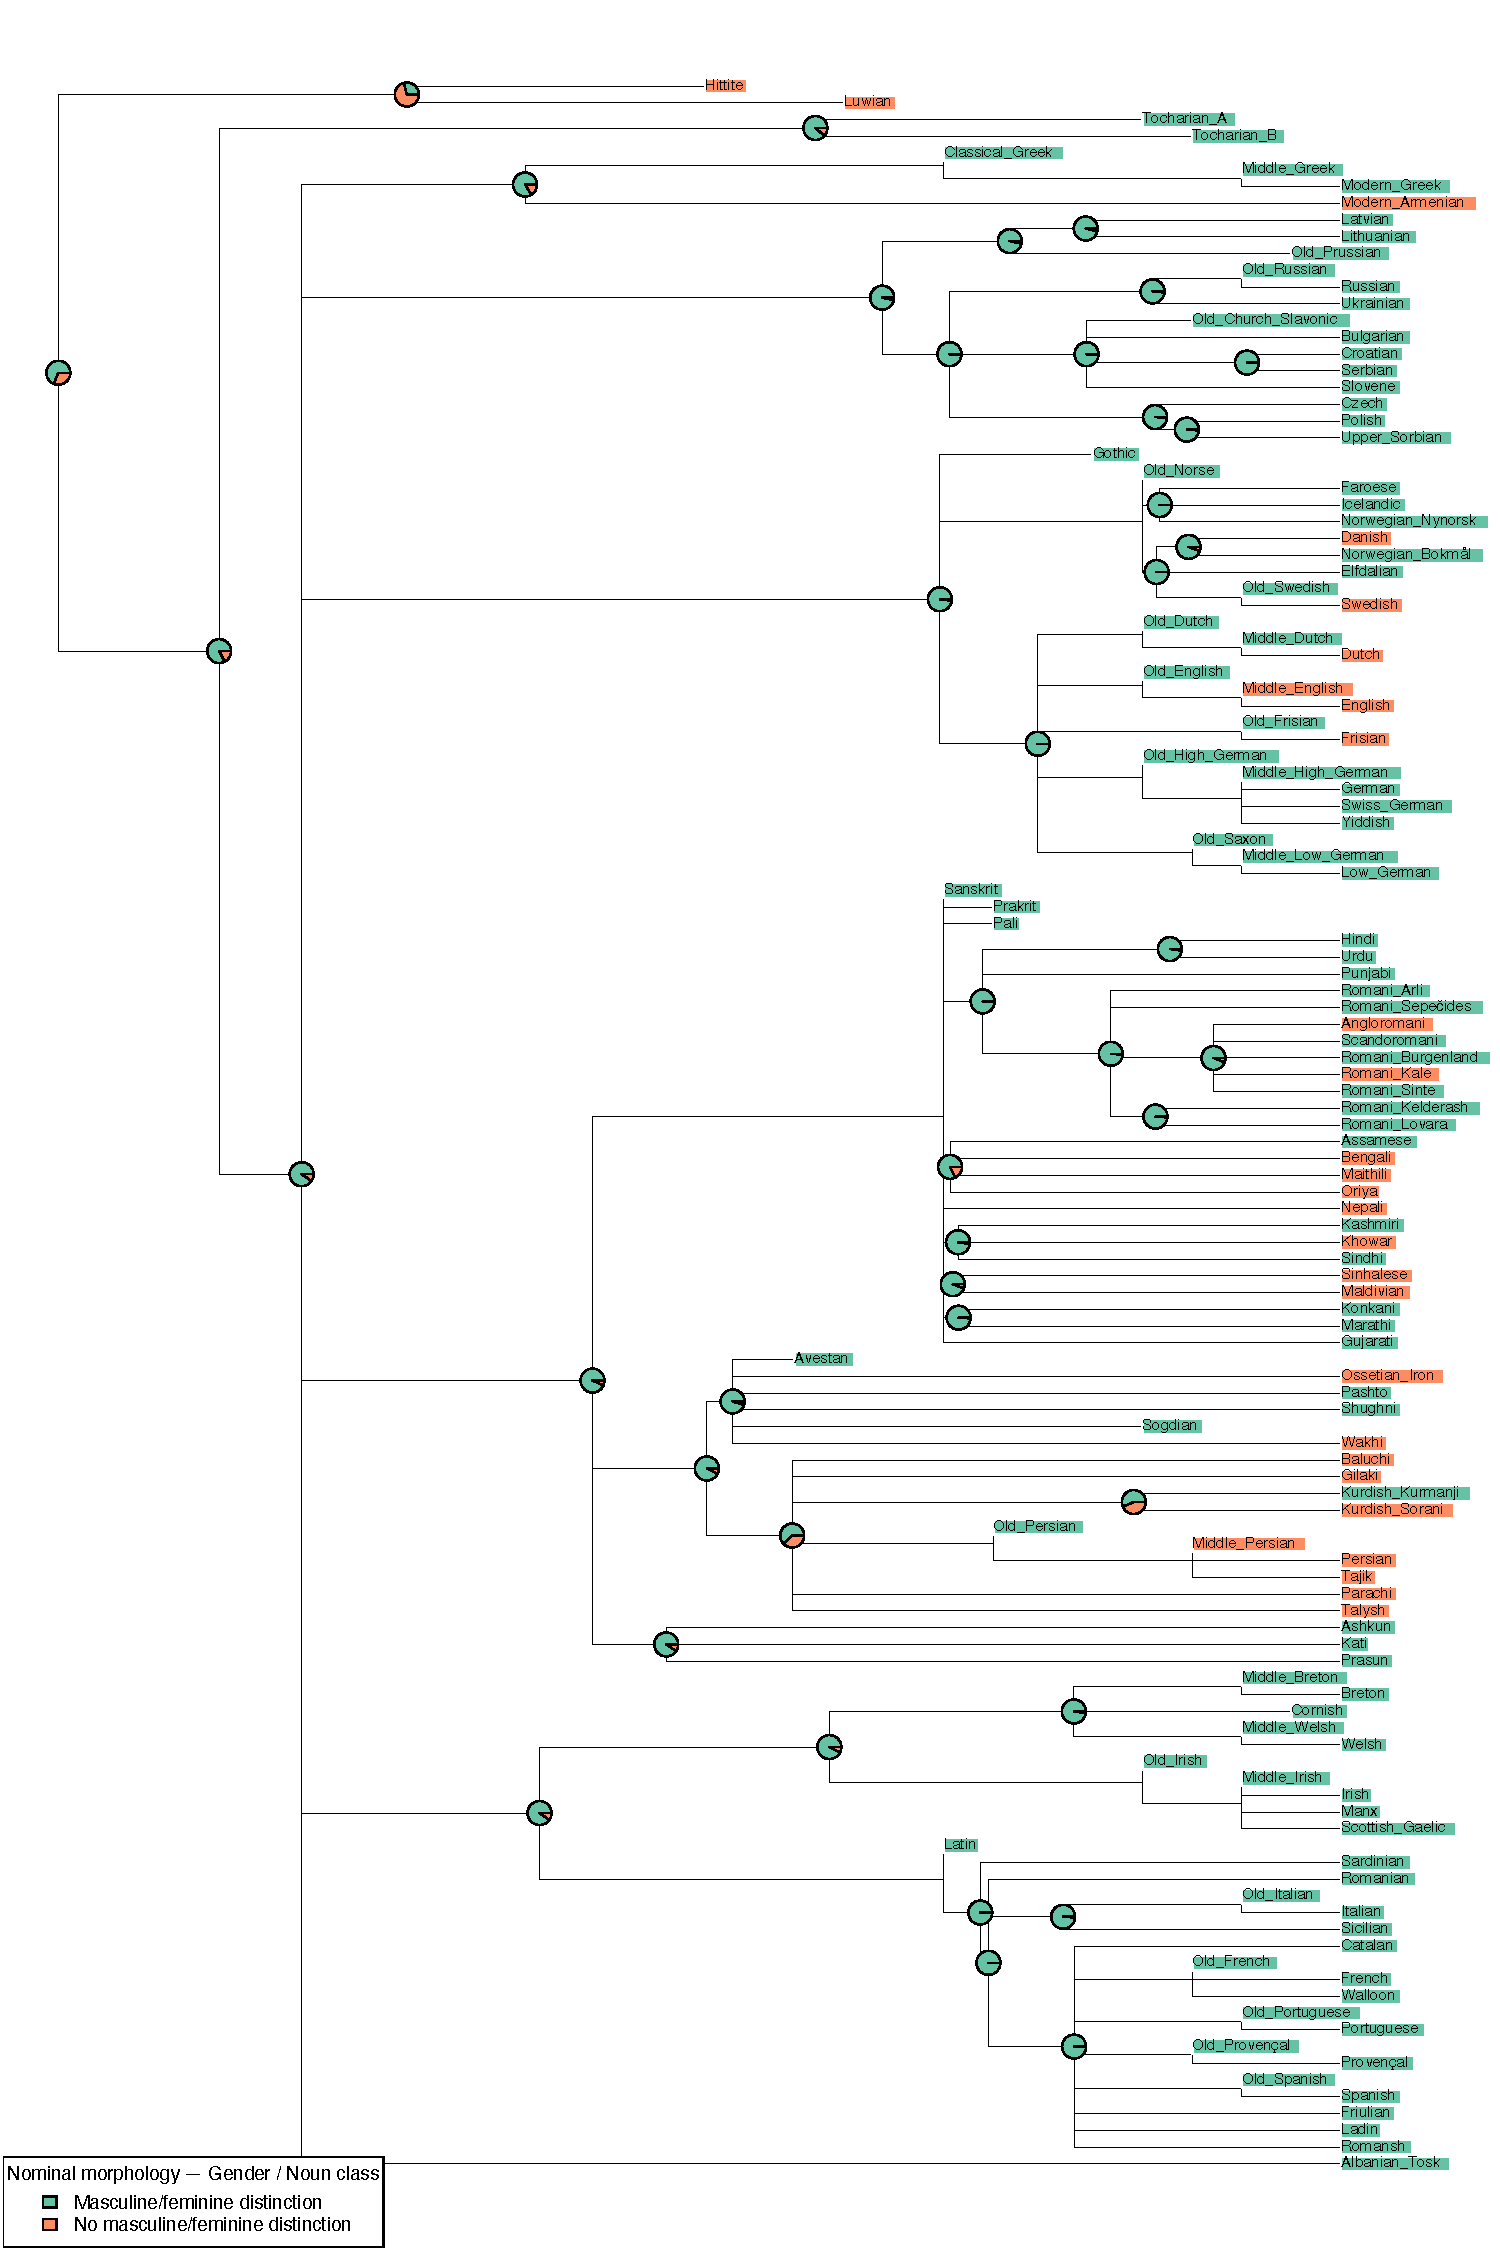
\includegraphics[width=.9\linewidth]{supp-graphics/NominalmorphologyGenderNounclassMF.pdf}

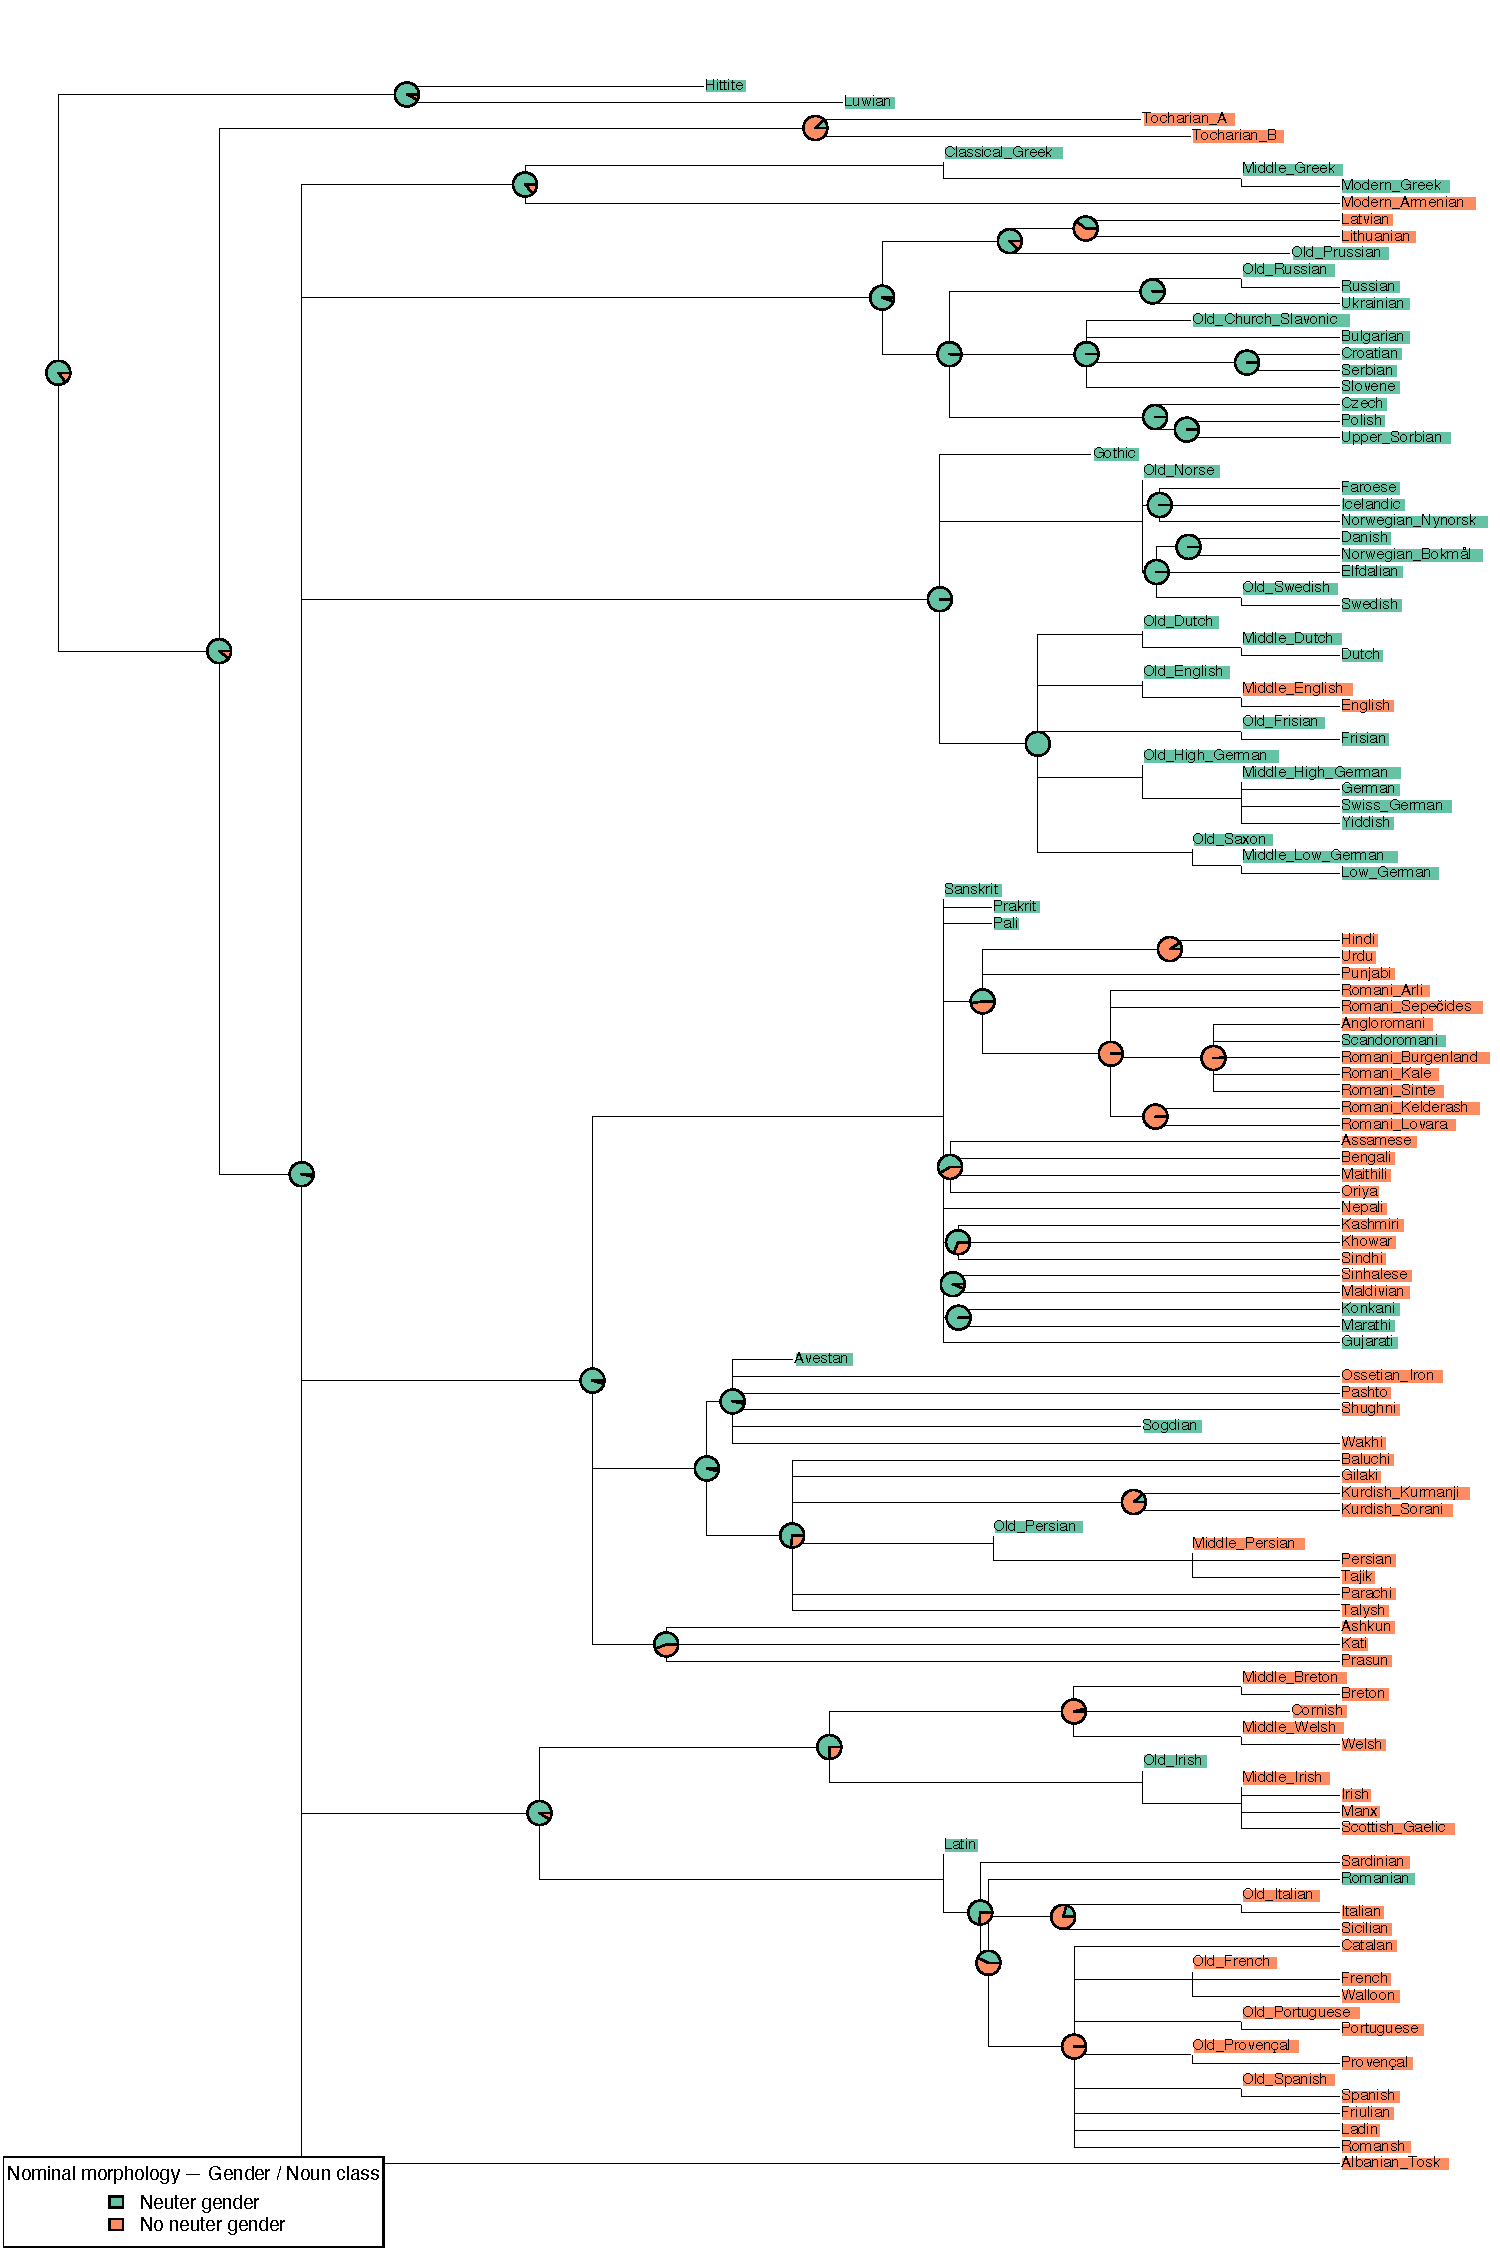
\includegraphics[width=.9\linewidth]{supp-graphics/NominalmorphologyGenderNounclassNEUTR.pdf}

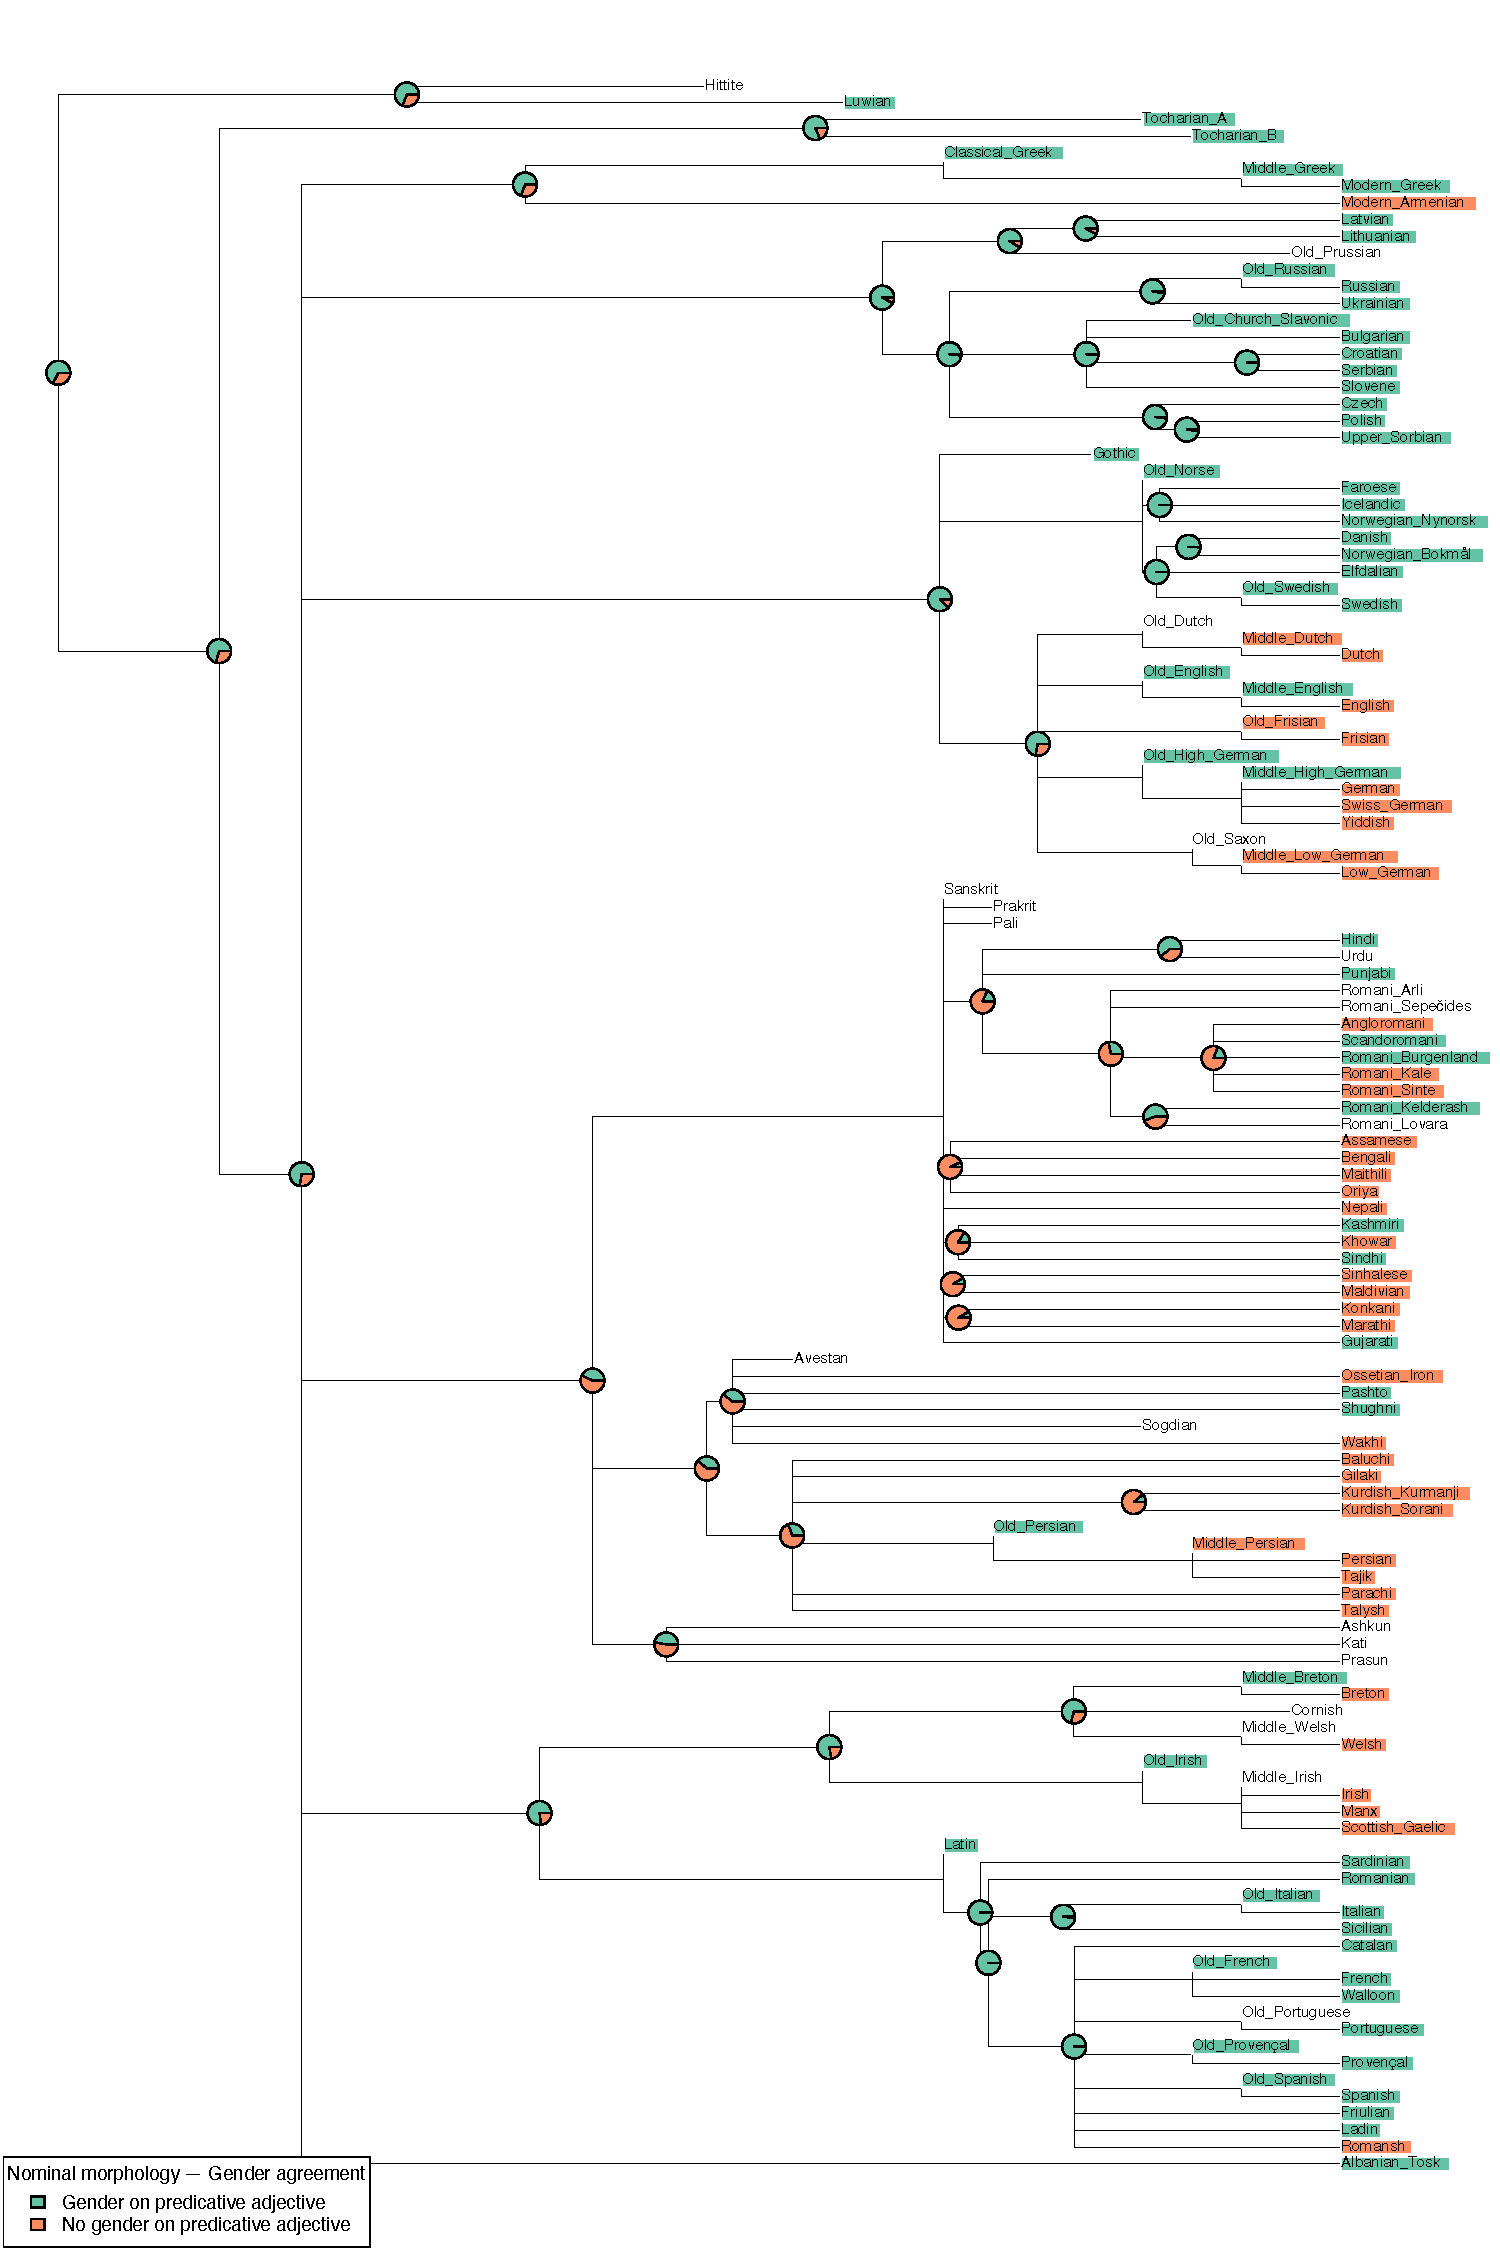
\includegraphics[width=.9\linewidth]{supp-graphics/NominalmorphologyGenderagreementPREDADJ.pdf}

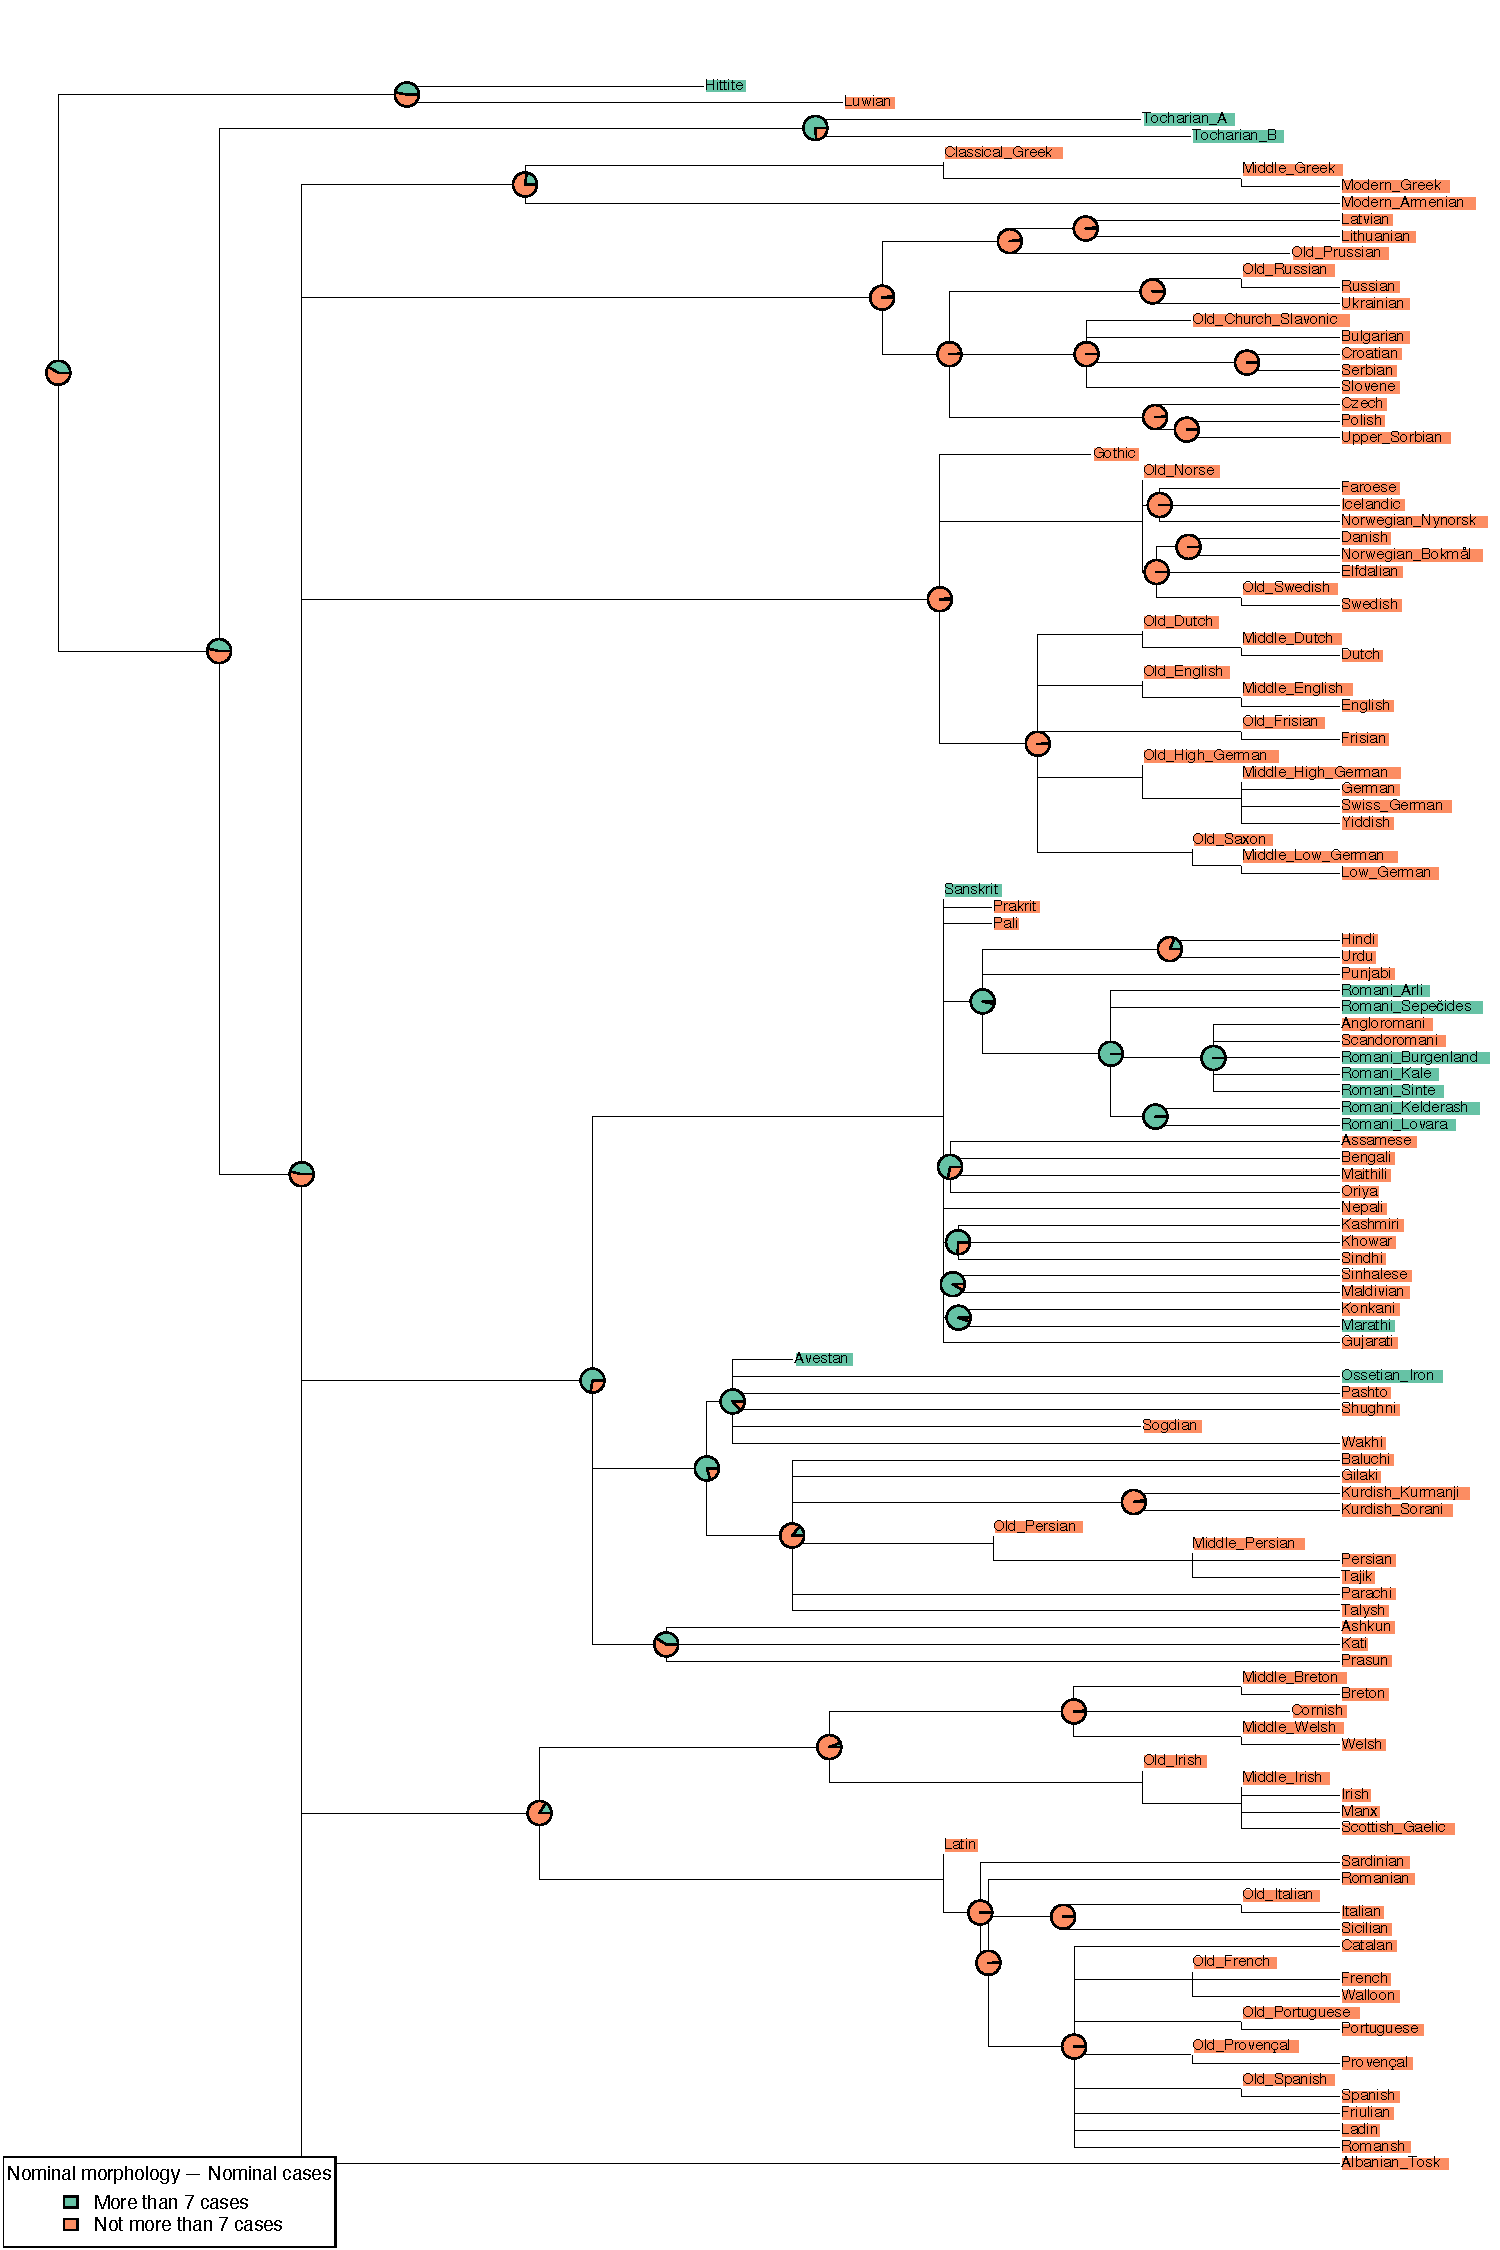
\includegraphics[width=.9\linewidth]{supp-graphics/NominalmorphologyNominalcases7Cases.pdf}

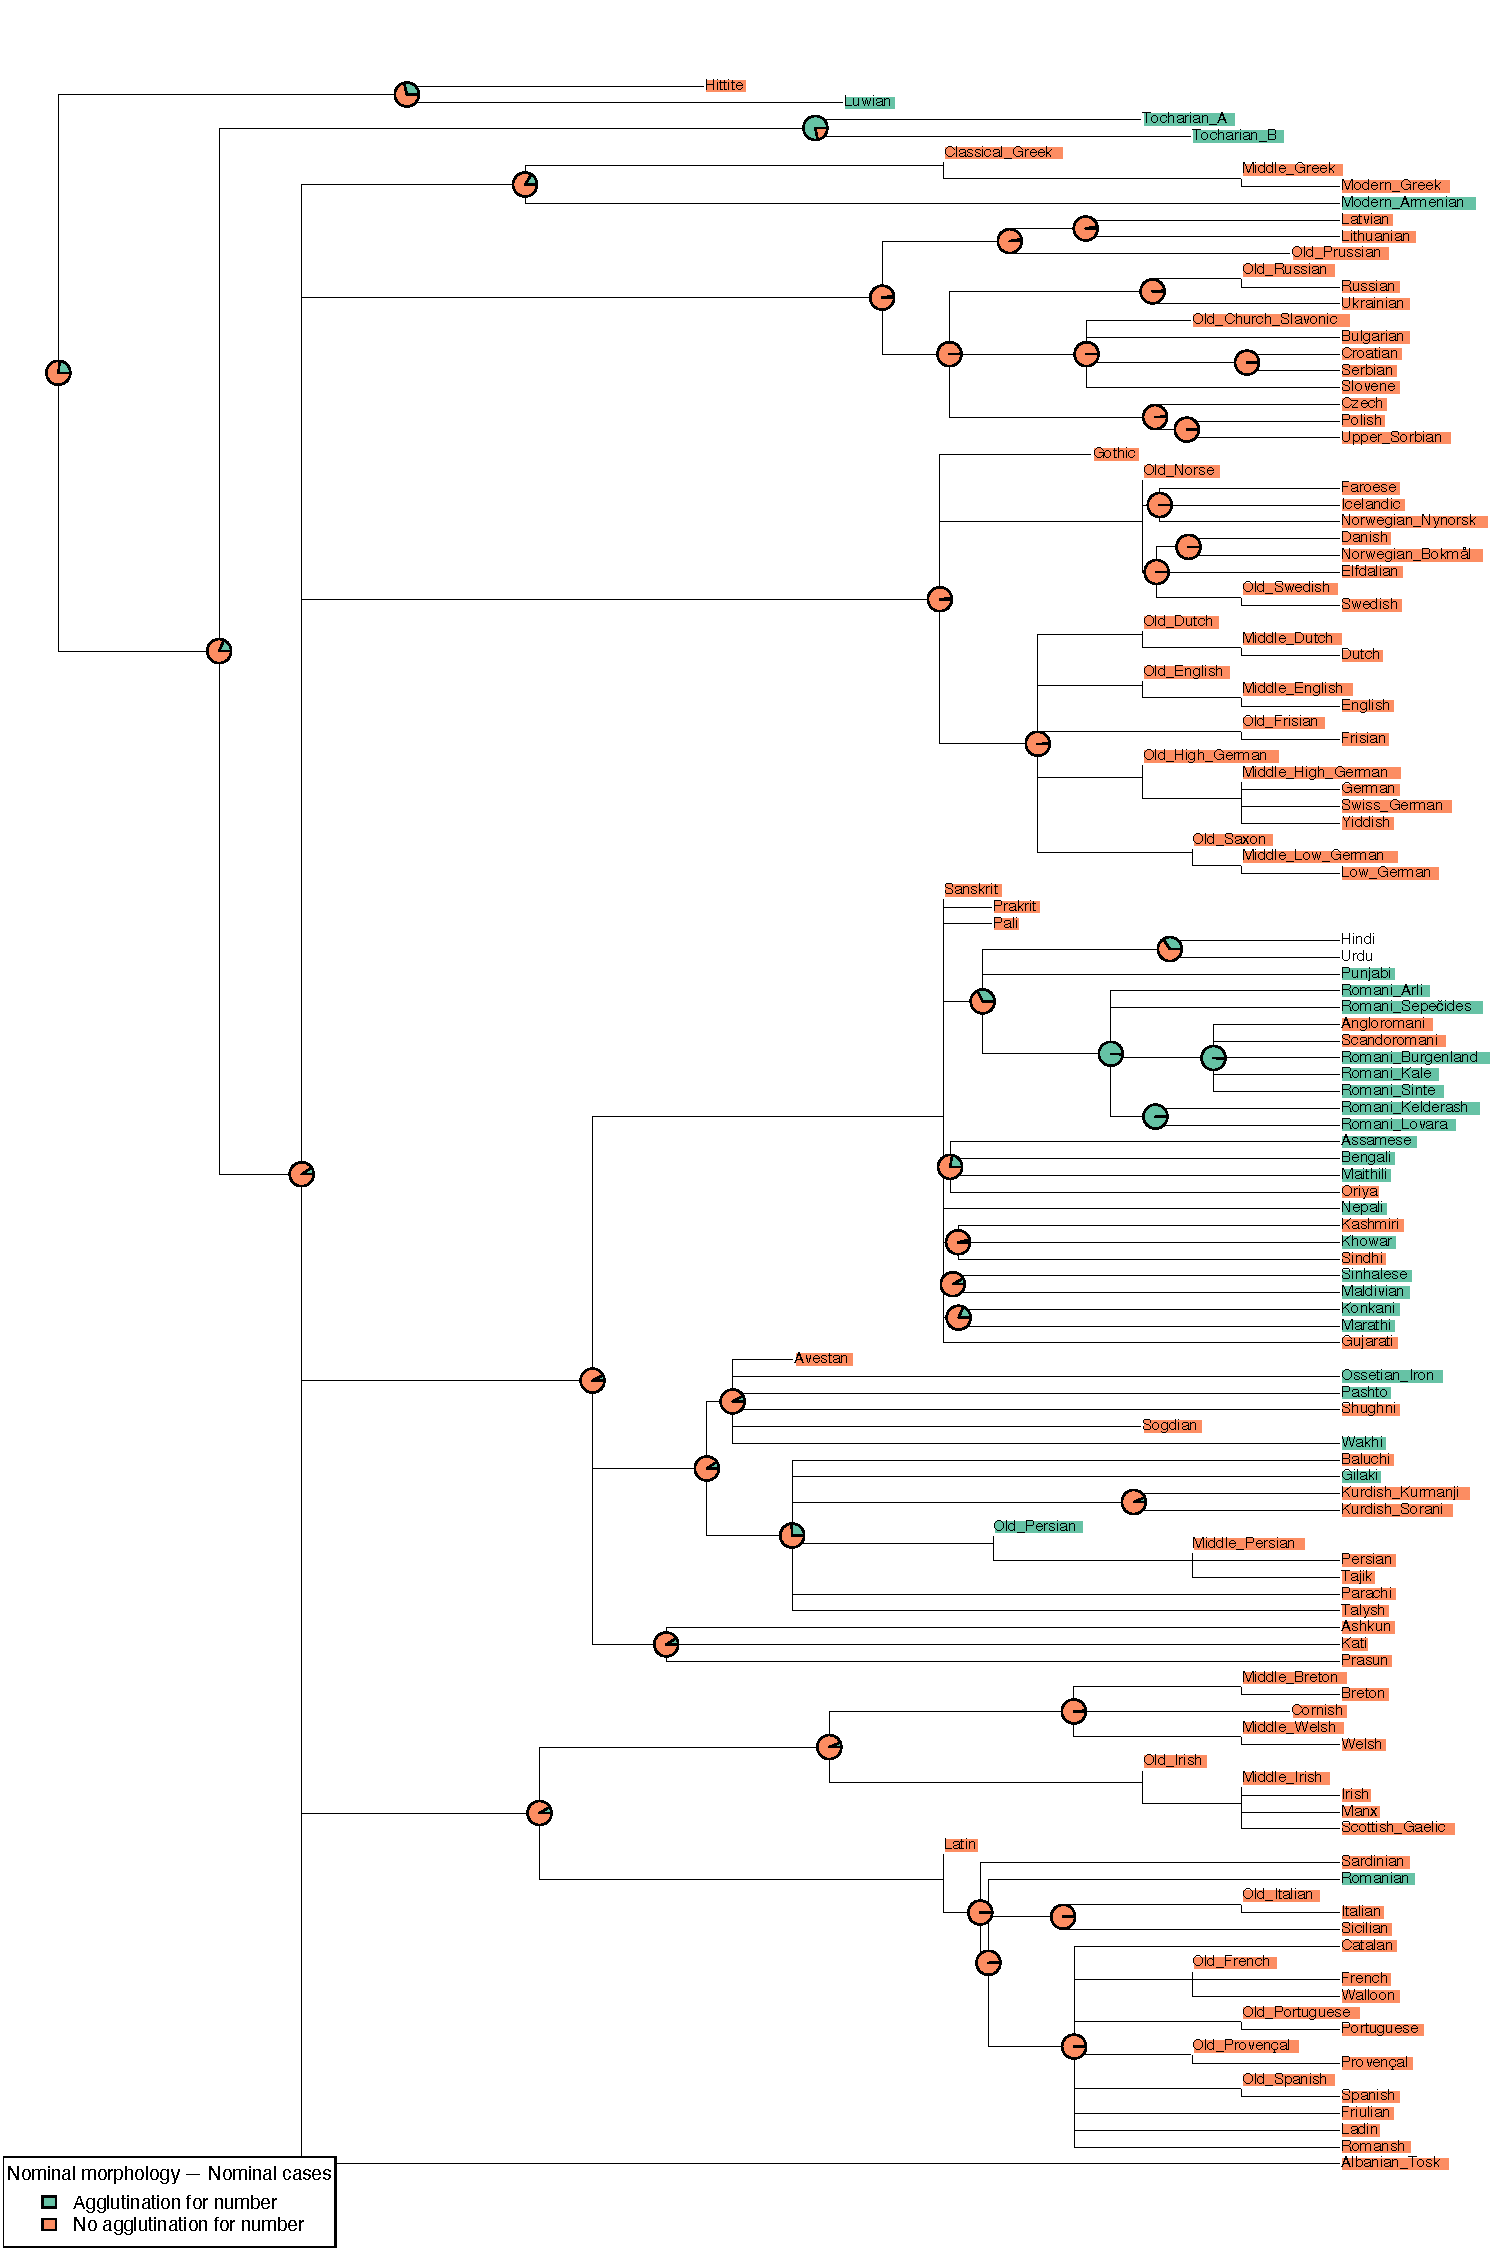
\includegraphics[width=.9\linewidth]{supp-graphics/NominalmorphologyNominalcasesAGGCASENR.pdf}

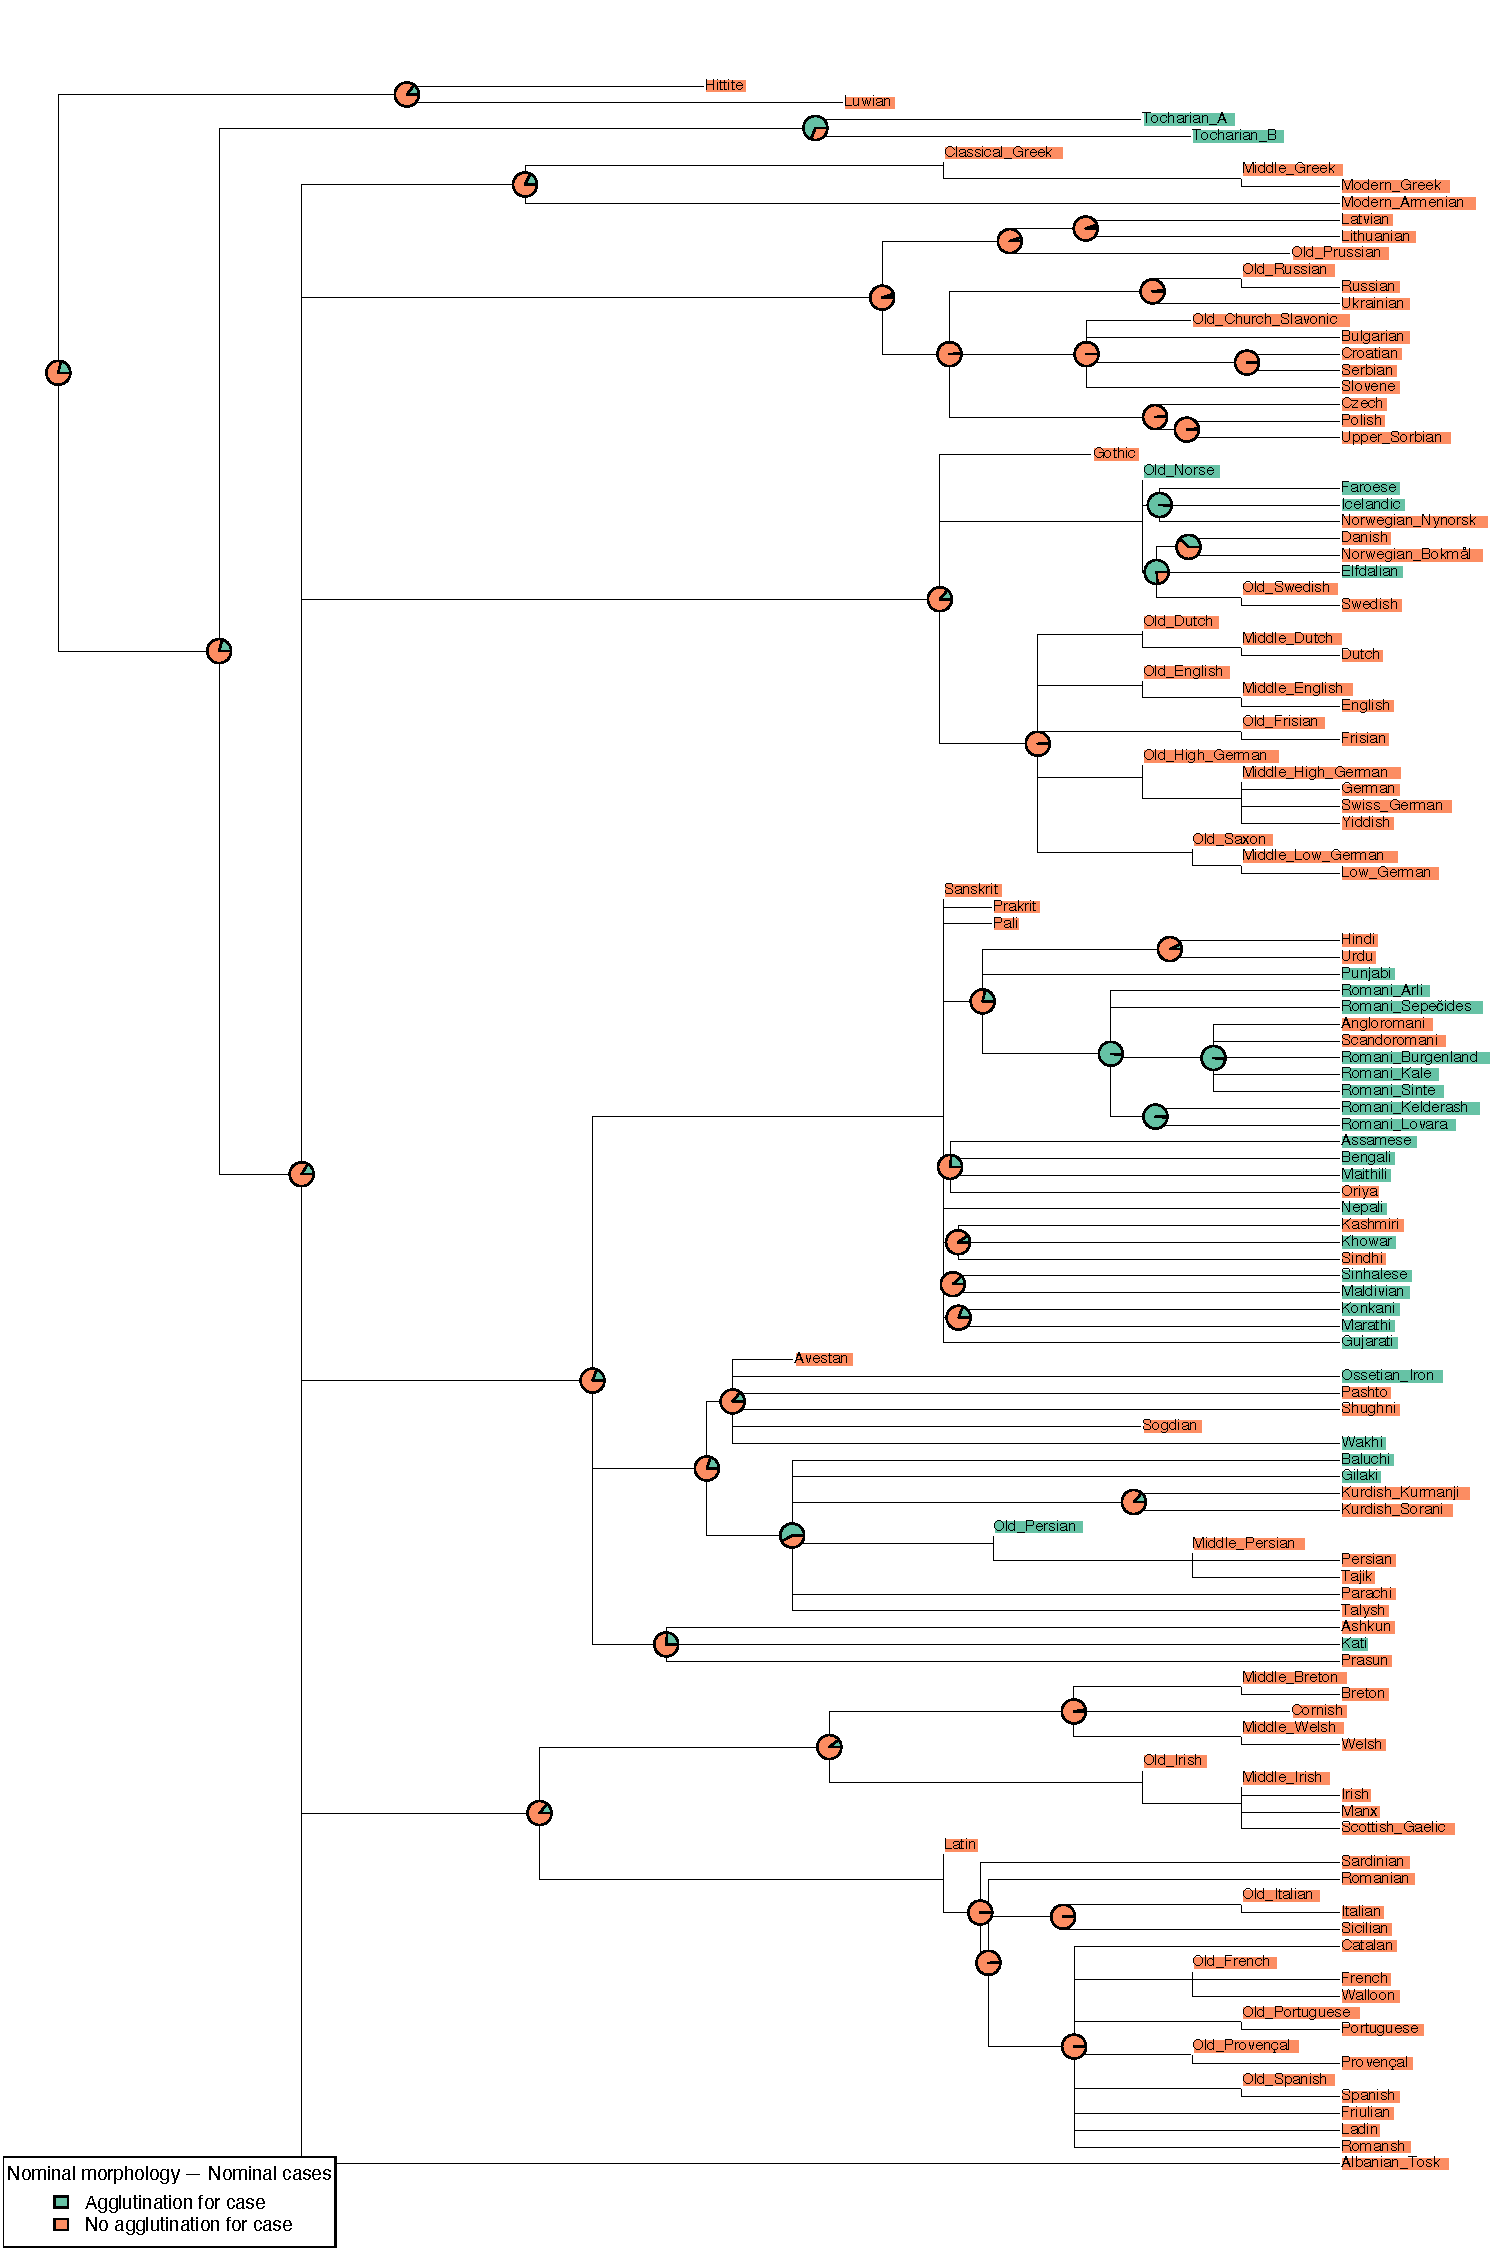
\includegraphics[width=.9\linewidth]{supp-graphics/NominalmorphologyNominalcasesAGGLCASE.pdf}

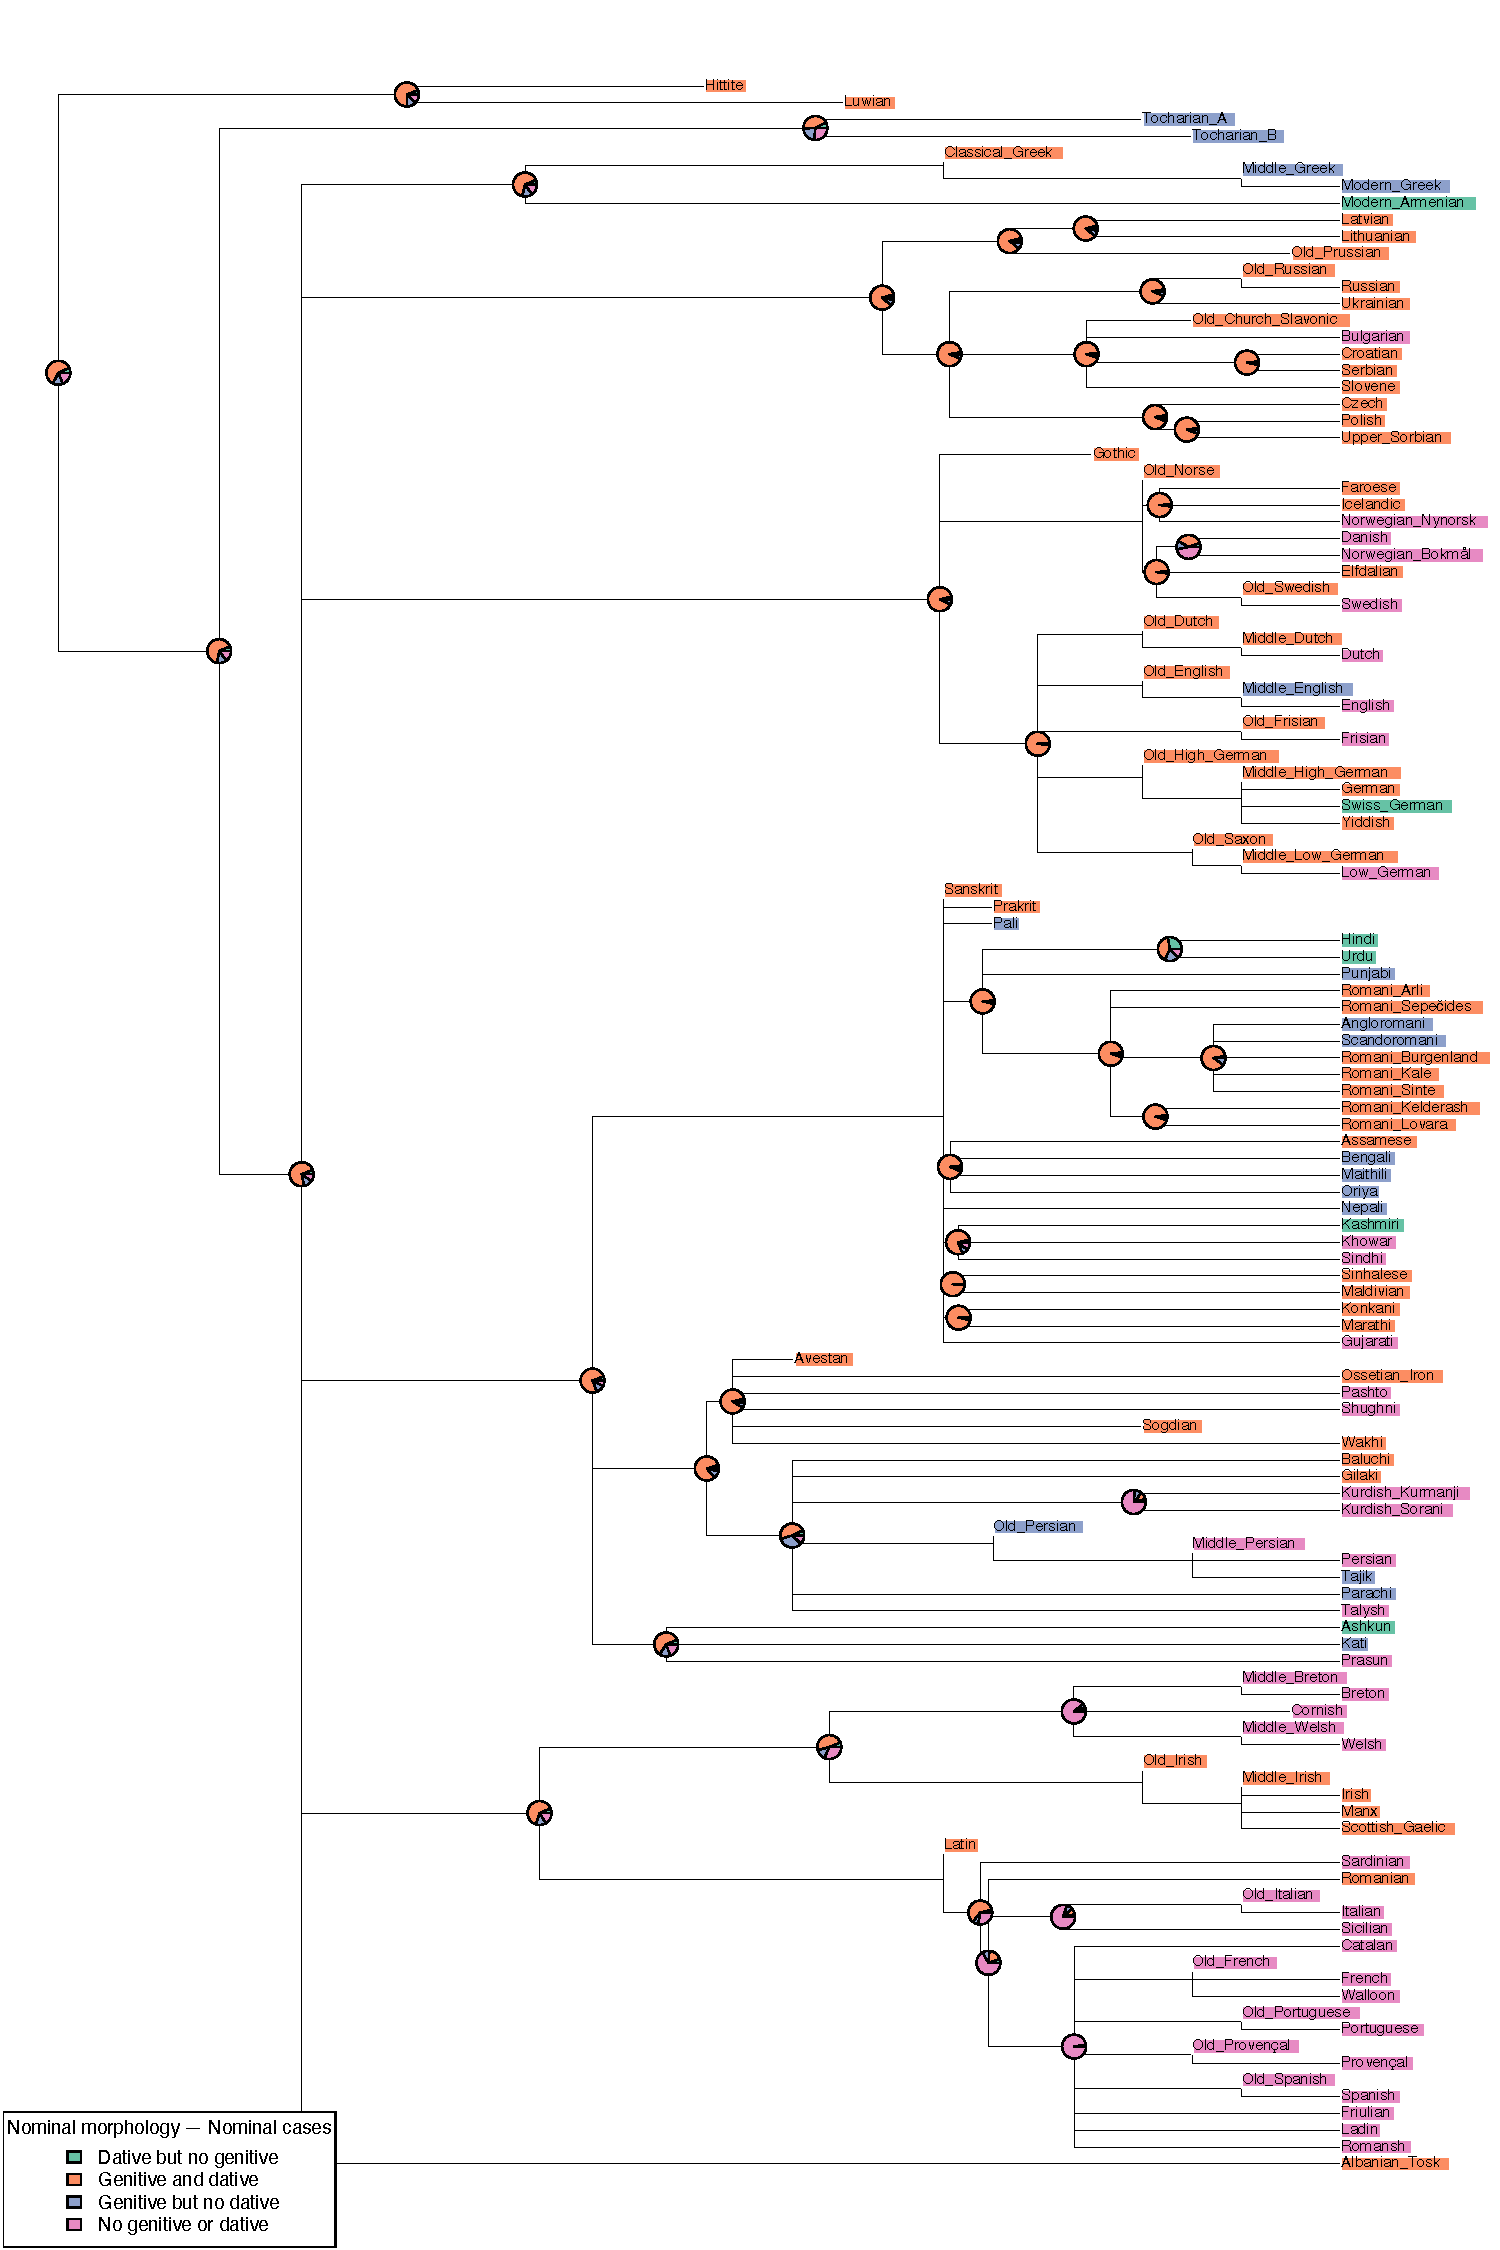
\includegraphics[width=.9\linewidth]{supp-graphics/NominalmorphologyNominalcasesDATNominalmorphologyNominalcasesGENNominalmorphologyNominalcasesGENDAT.pdf}

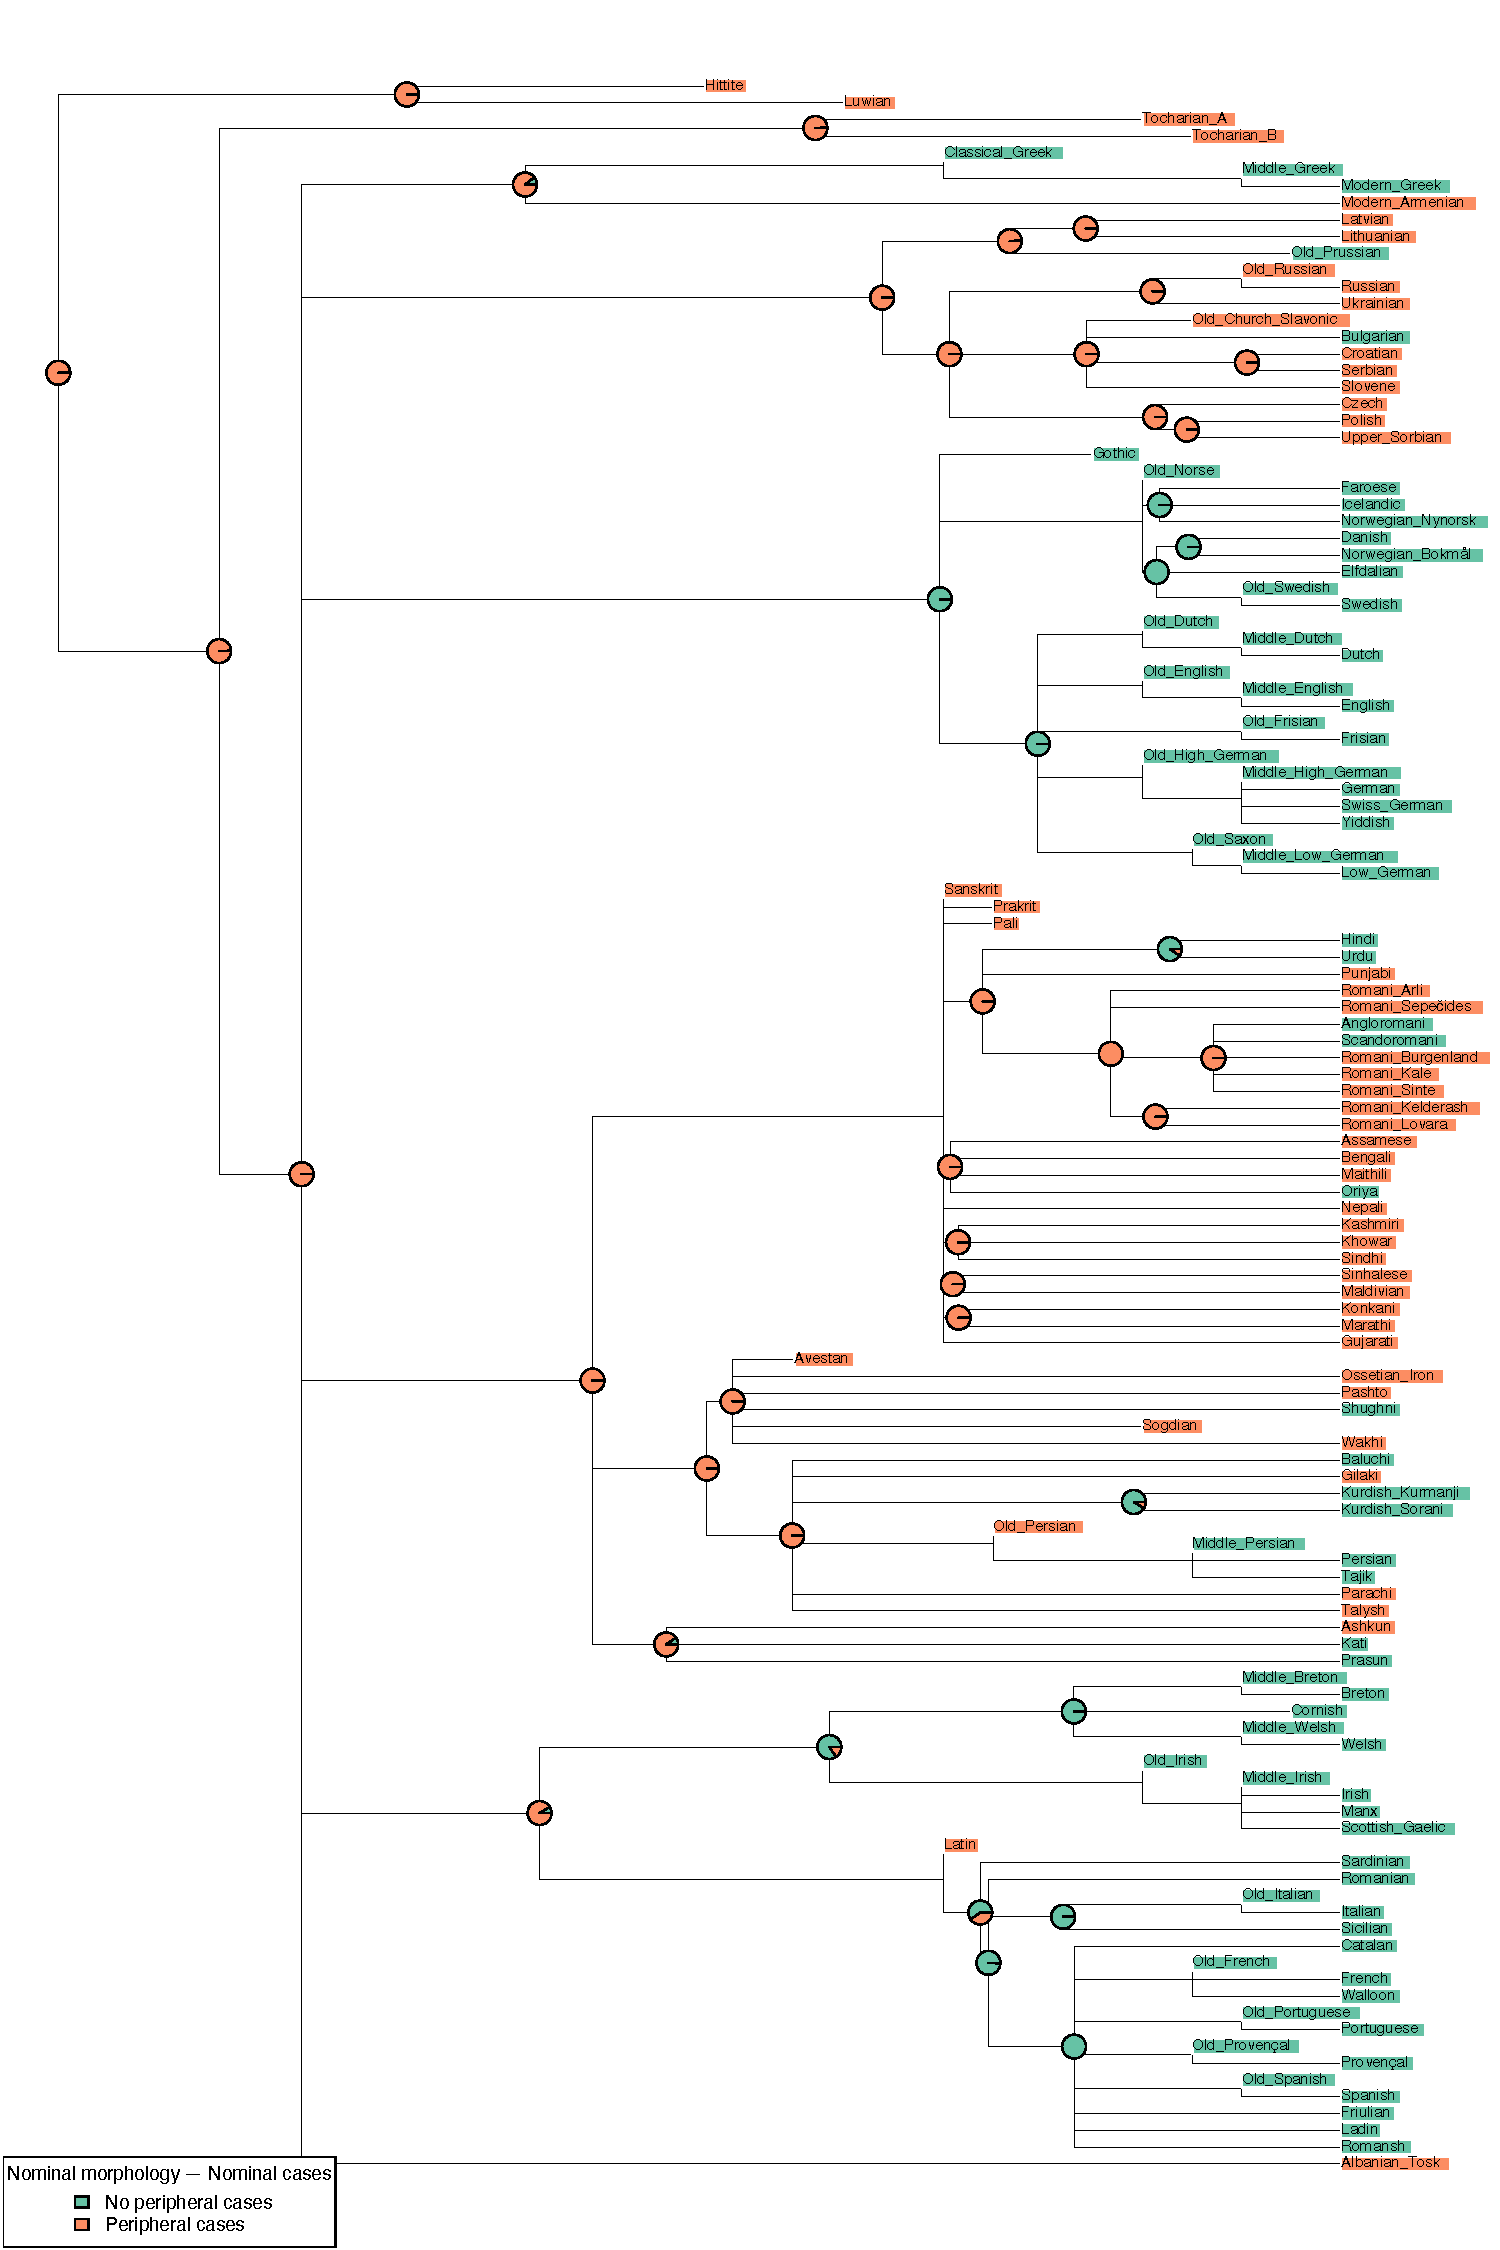
\includegraphics[width=.9\linewidth]{supp-graphics/NominalmorphologyNominalcasesOBLCases.pdf}

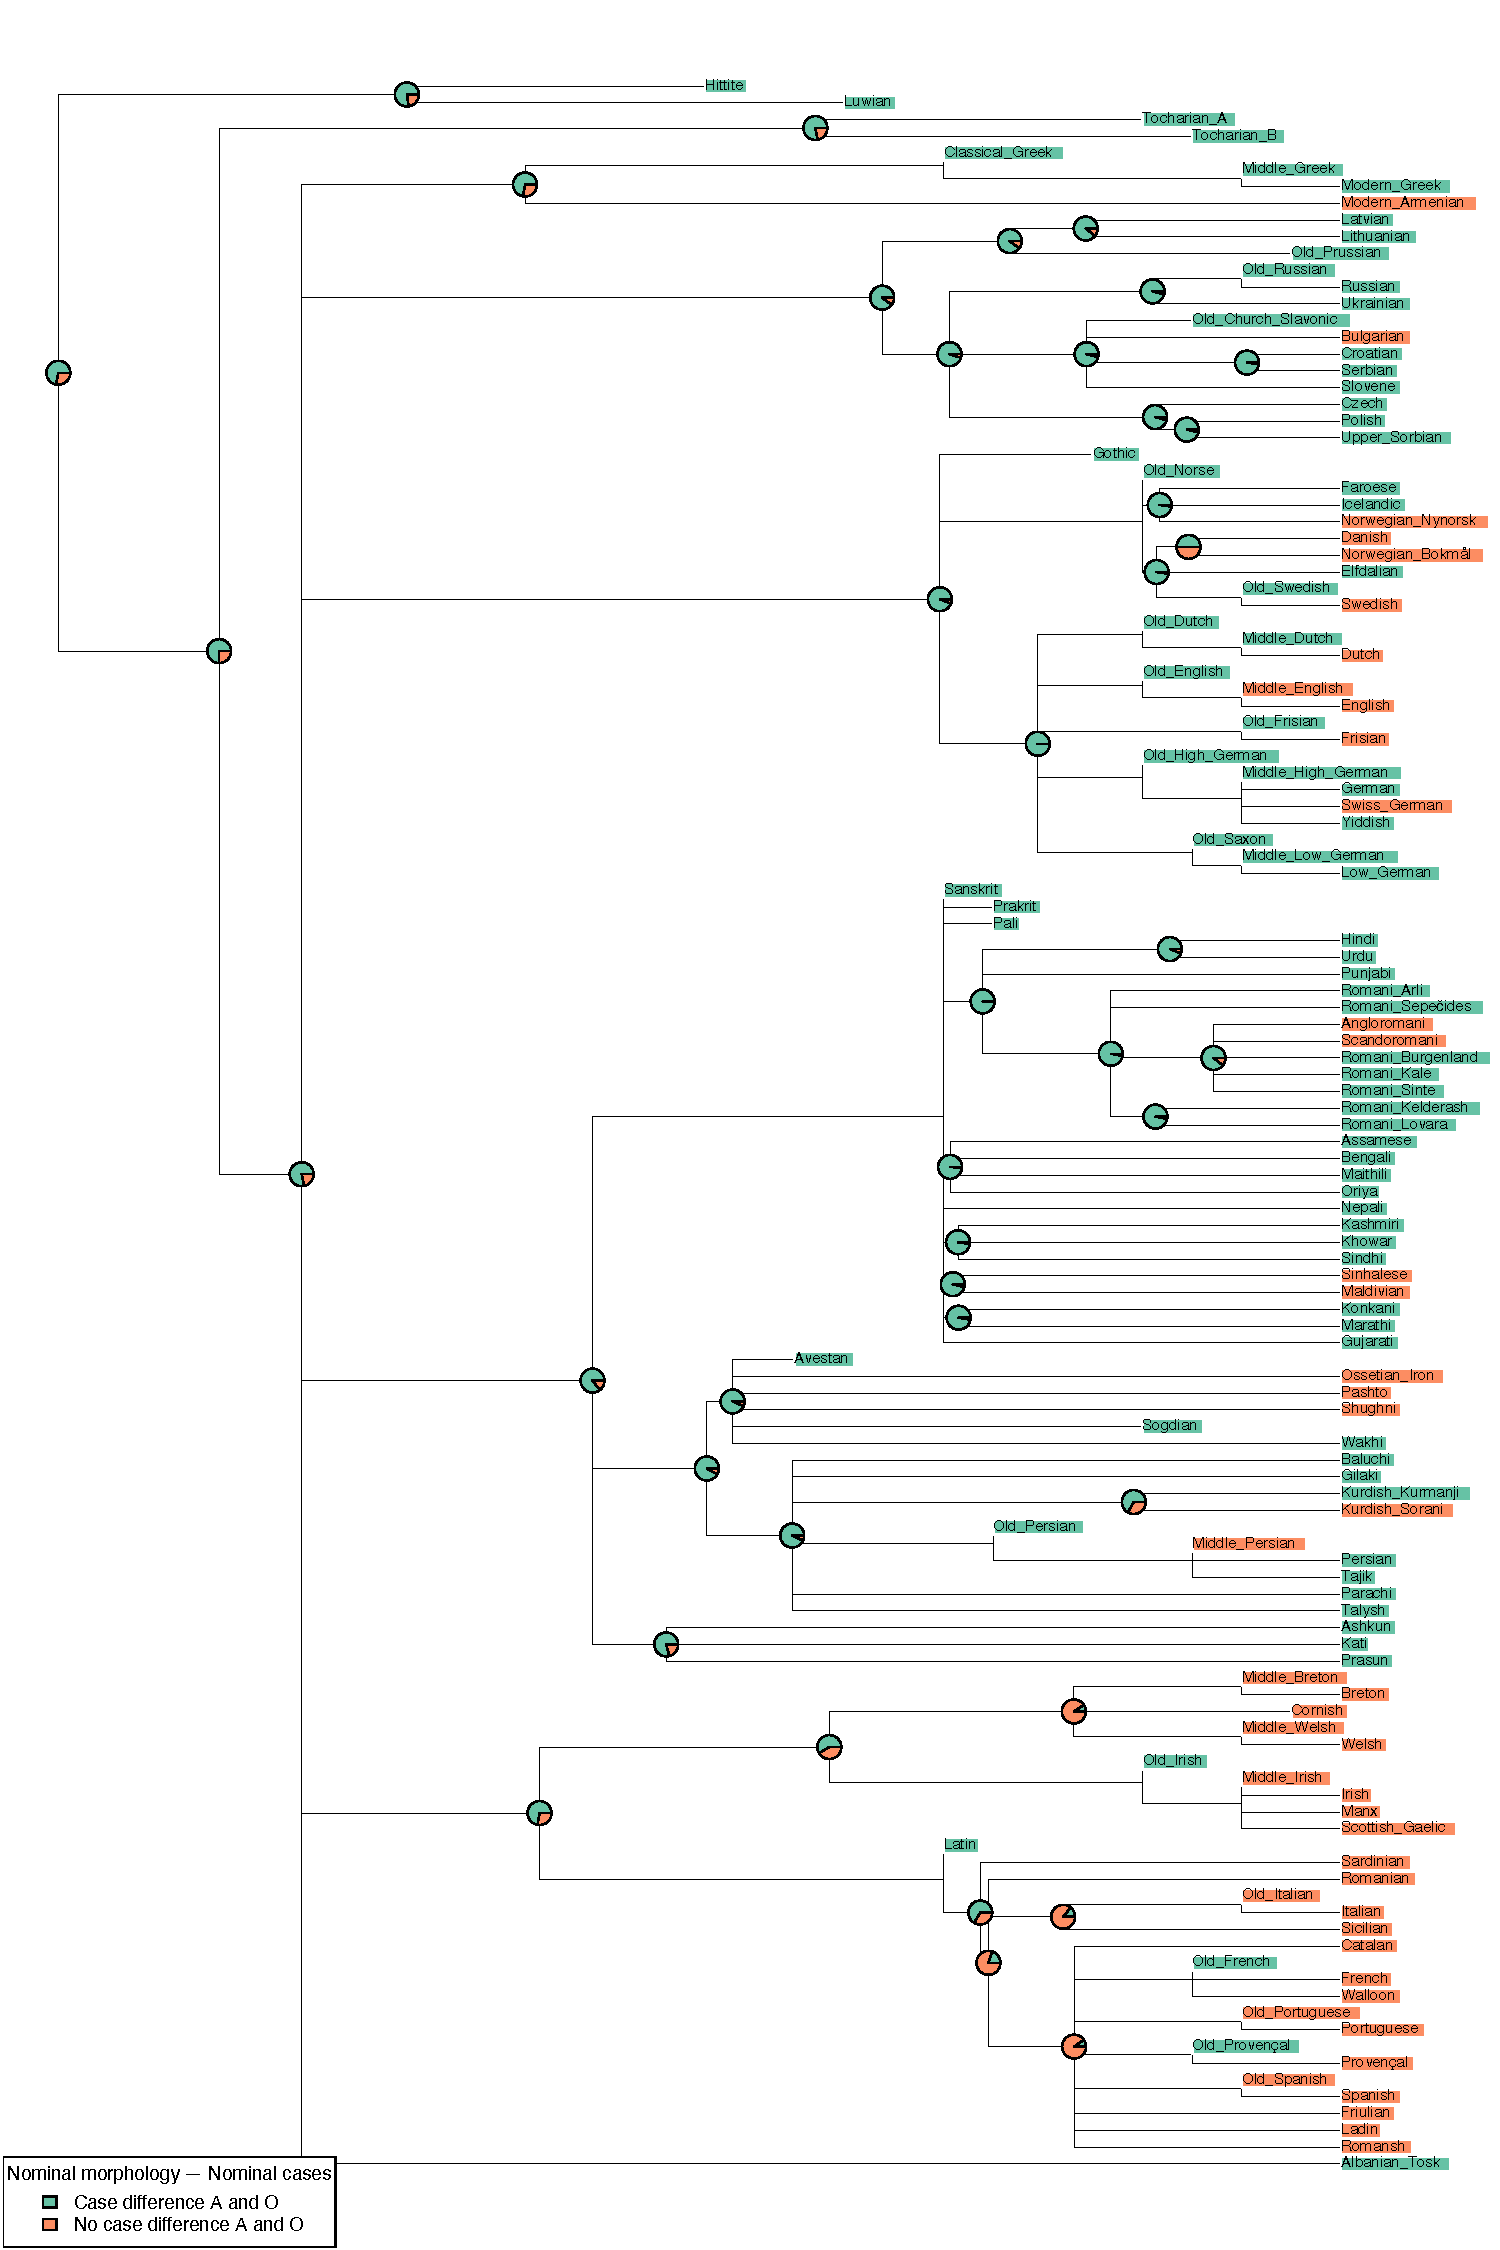
\includegraphics[width=.9\linewidth]{supp-graphics/NominalmorphologyNominalcasesOcase.pdf}

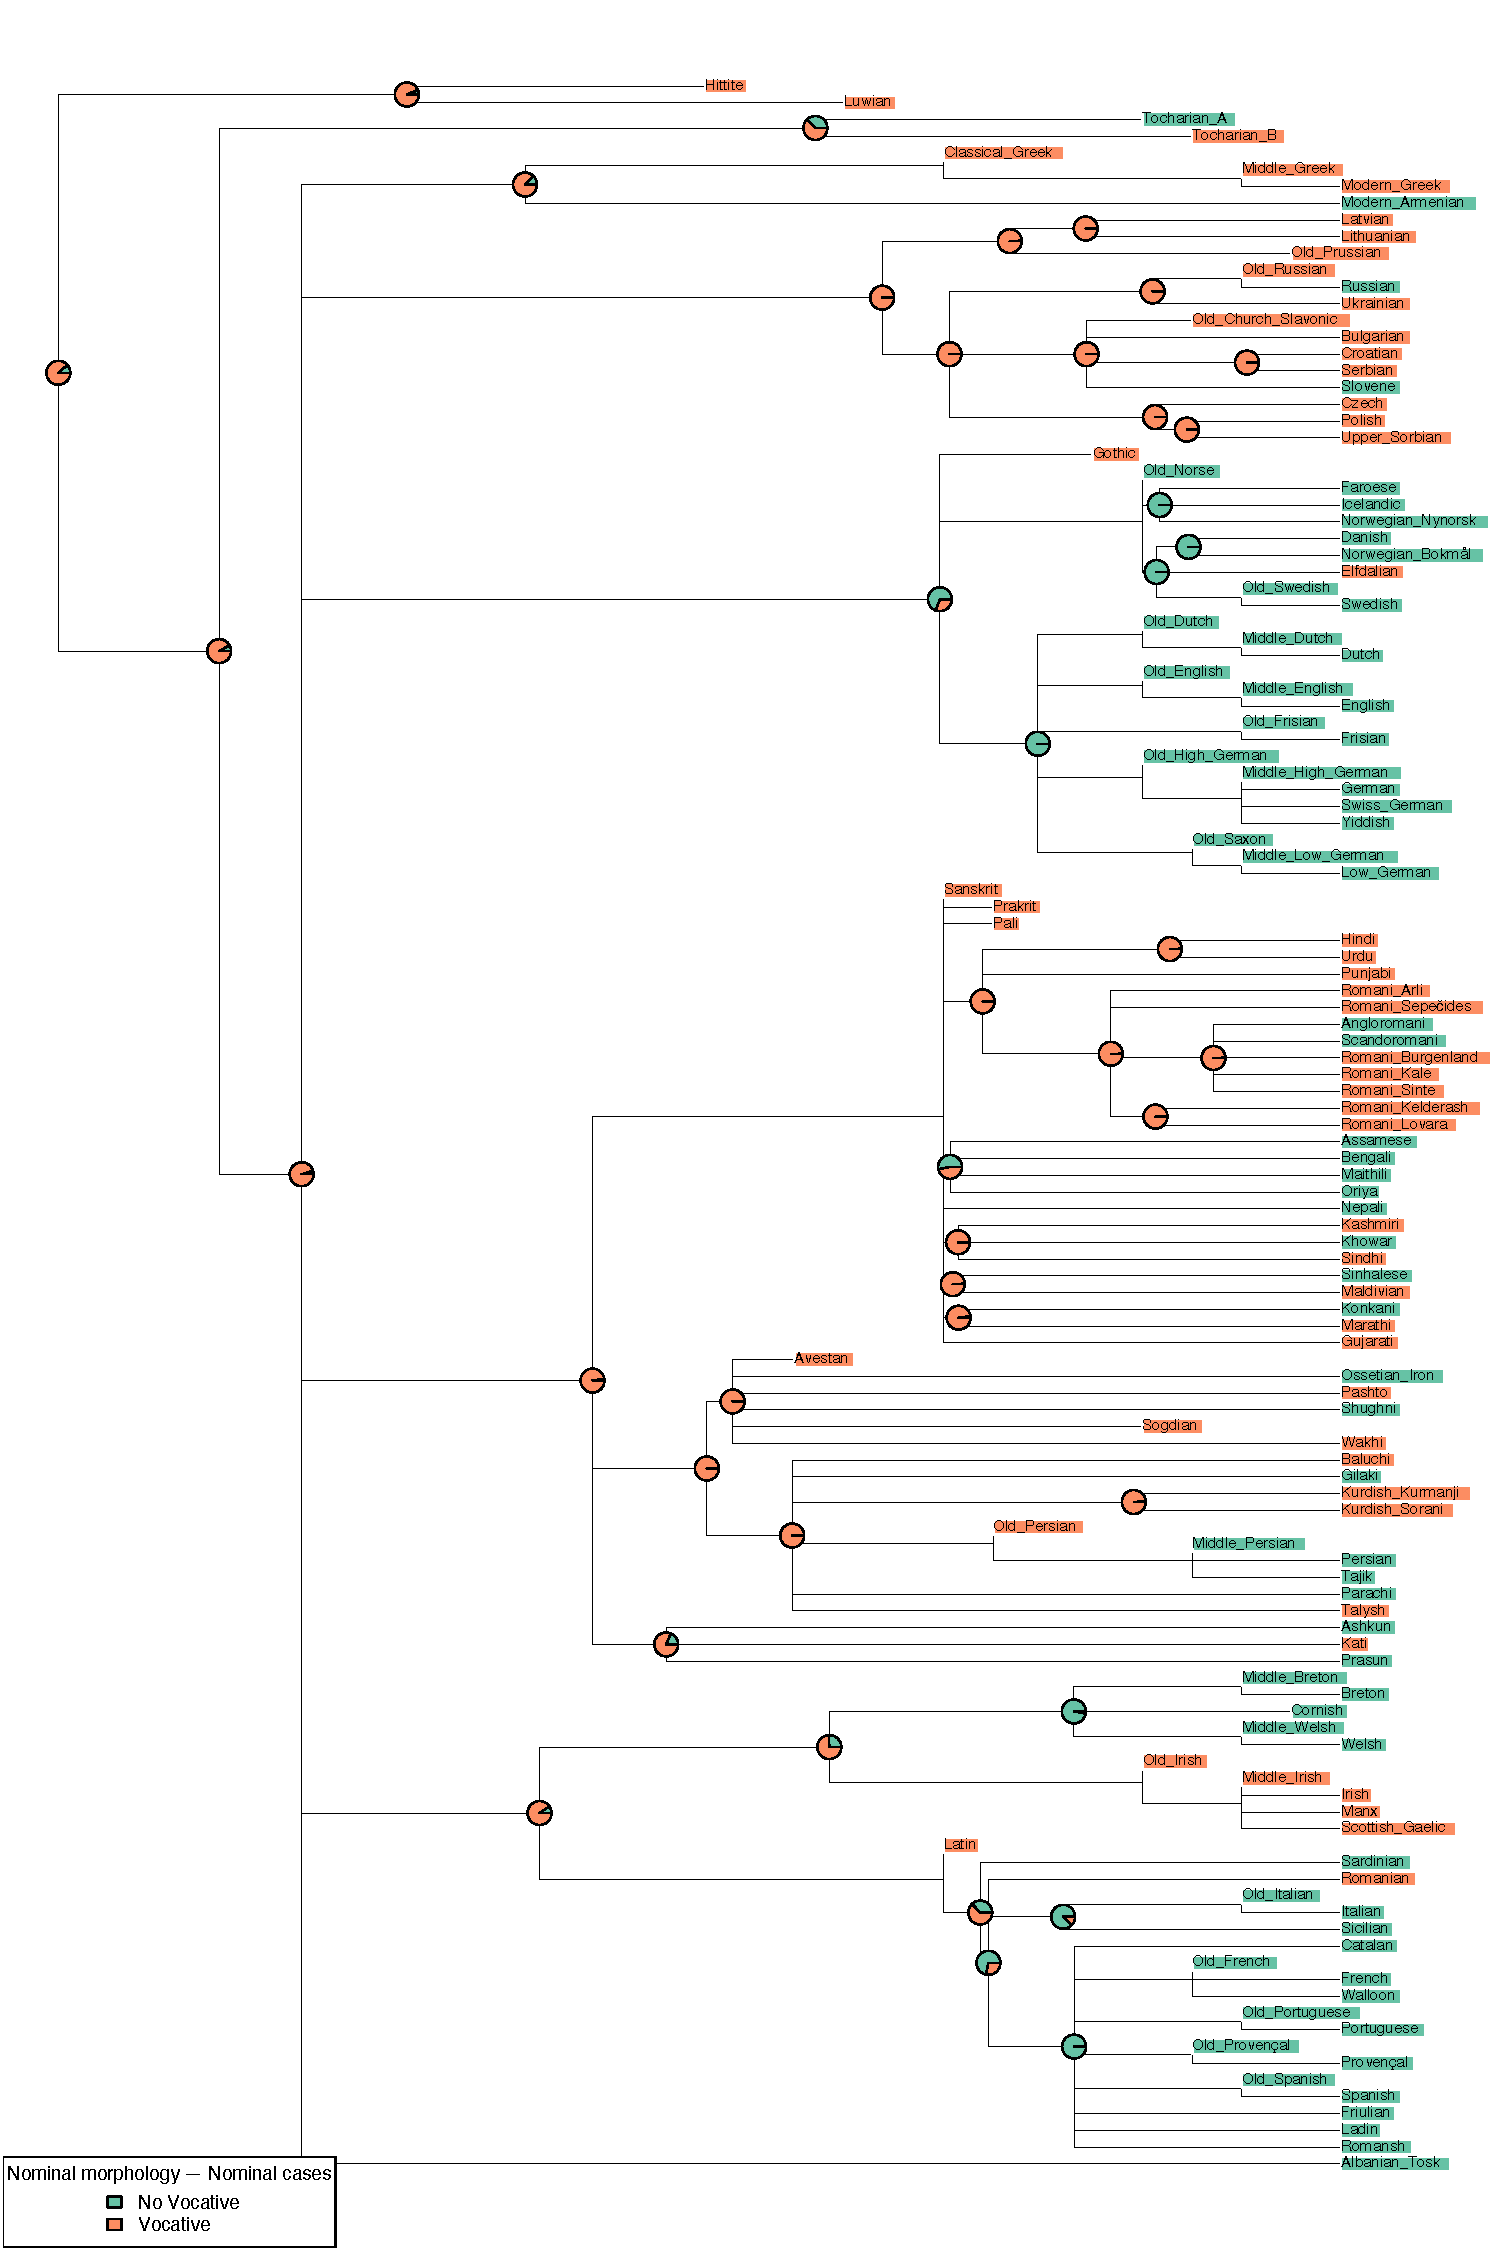
\includegraphics[width=.9\linewidth]{supp-graphics/NominalmorphologyNominalcasesVOC.pdf}

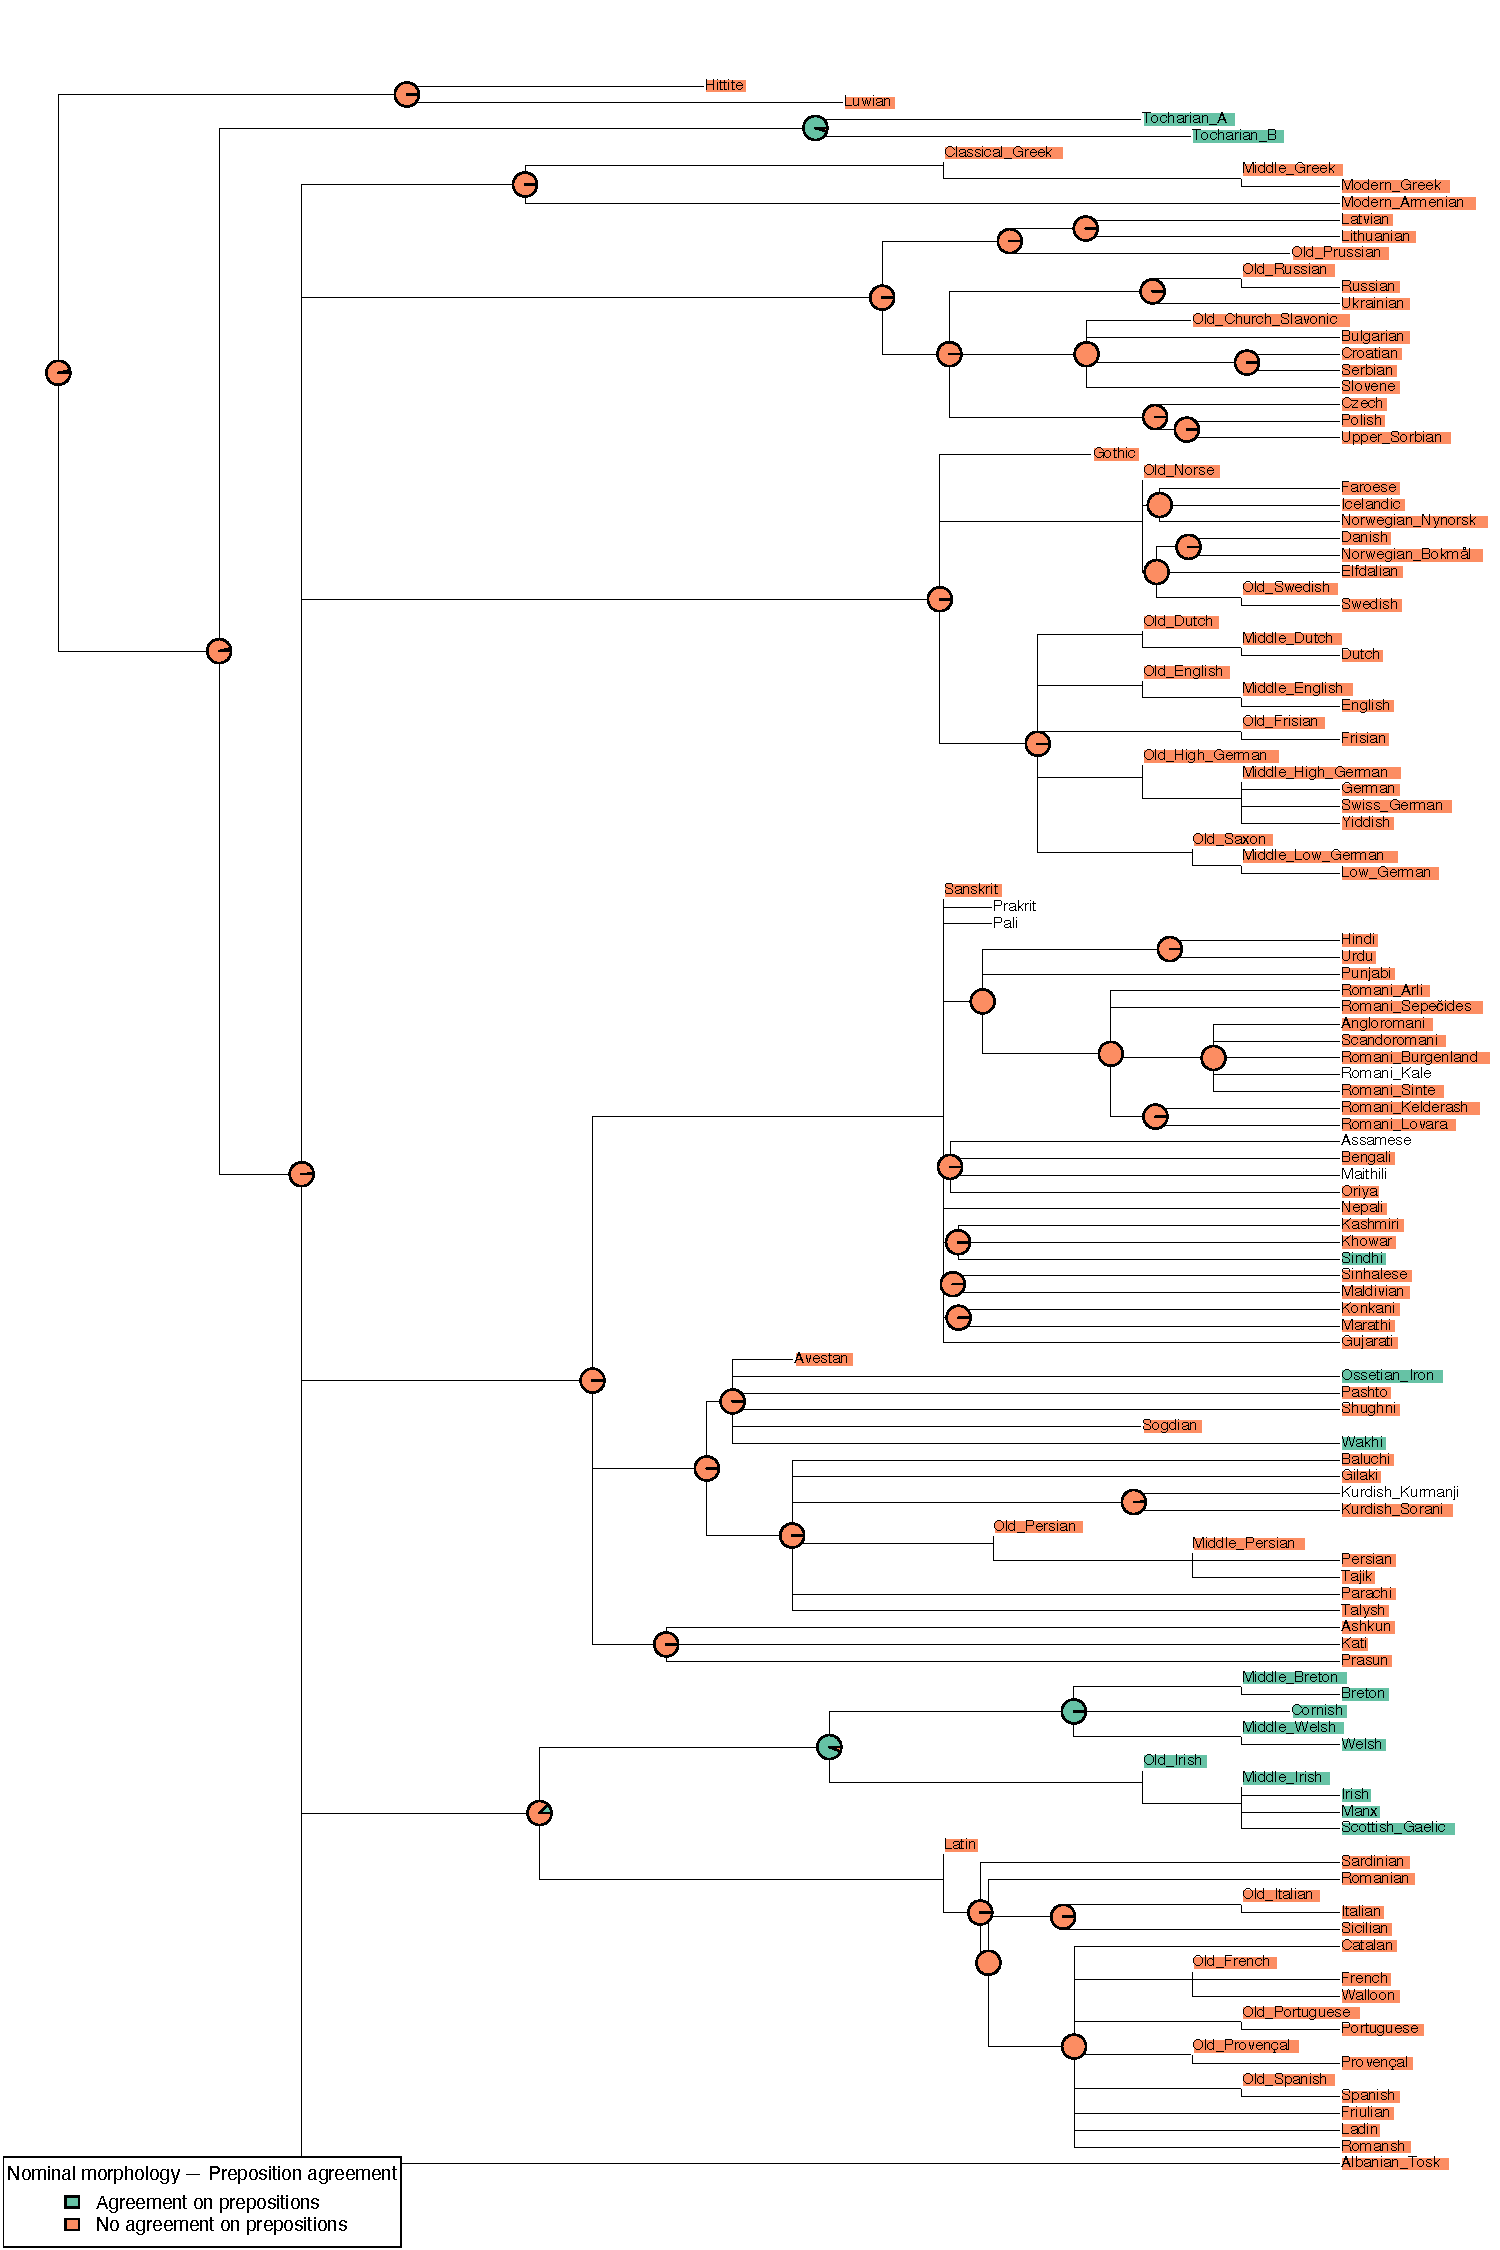
\includegraphics[width=.9\linewidth]{supp-graphics/NominalmorphologyPrepositionagreementPRONAGR.pdf}

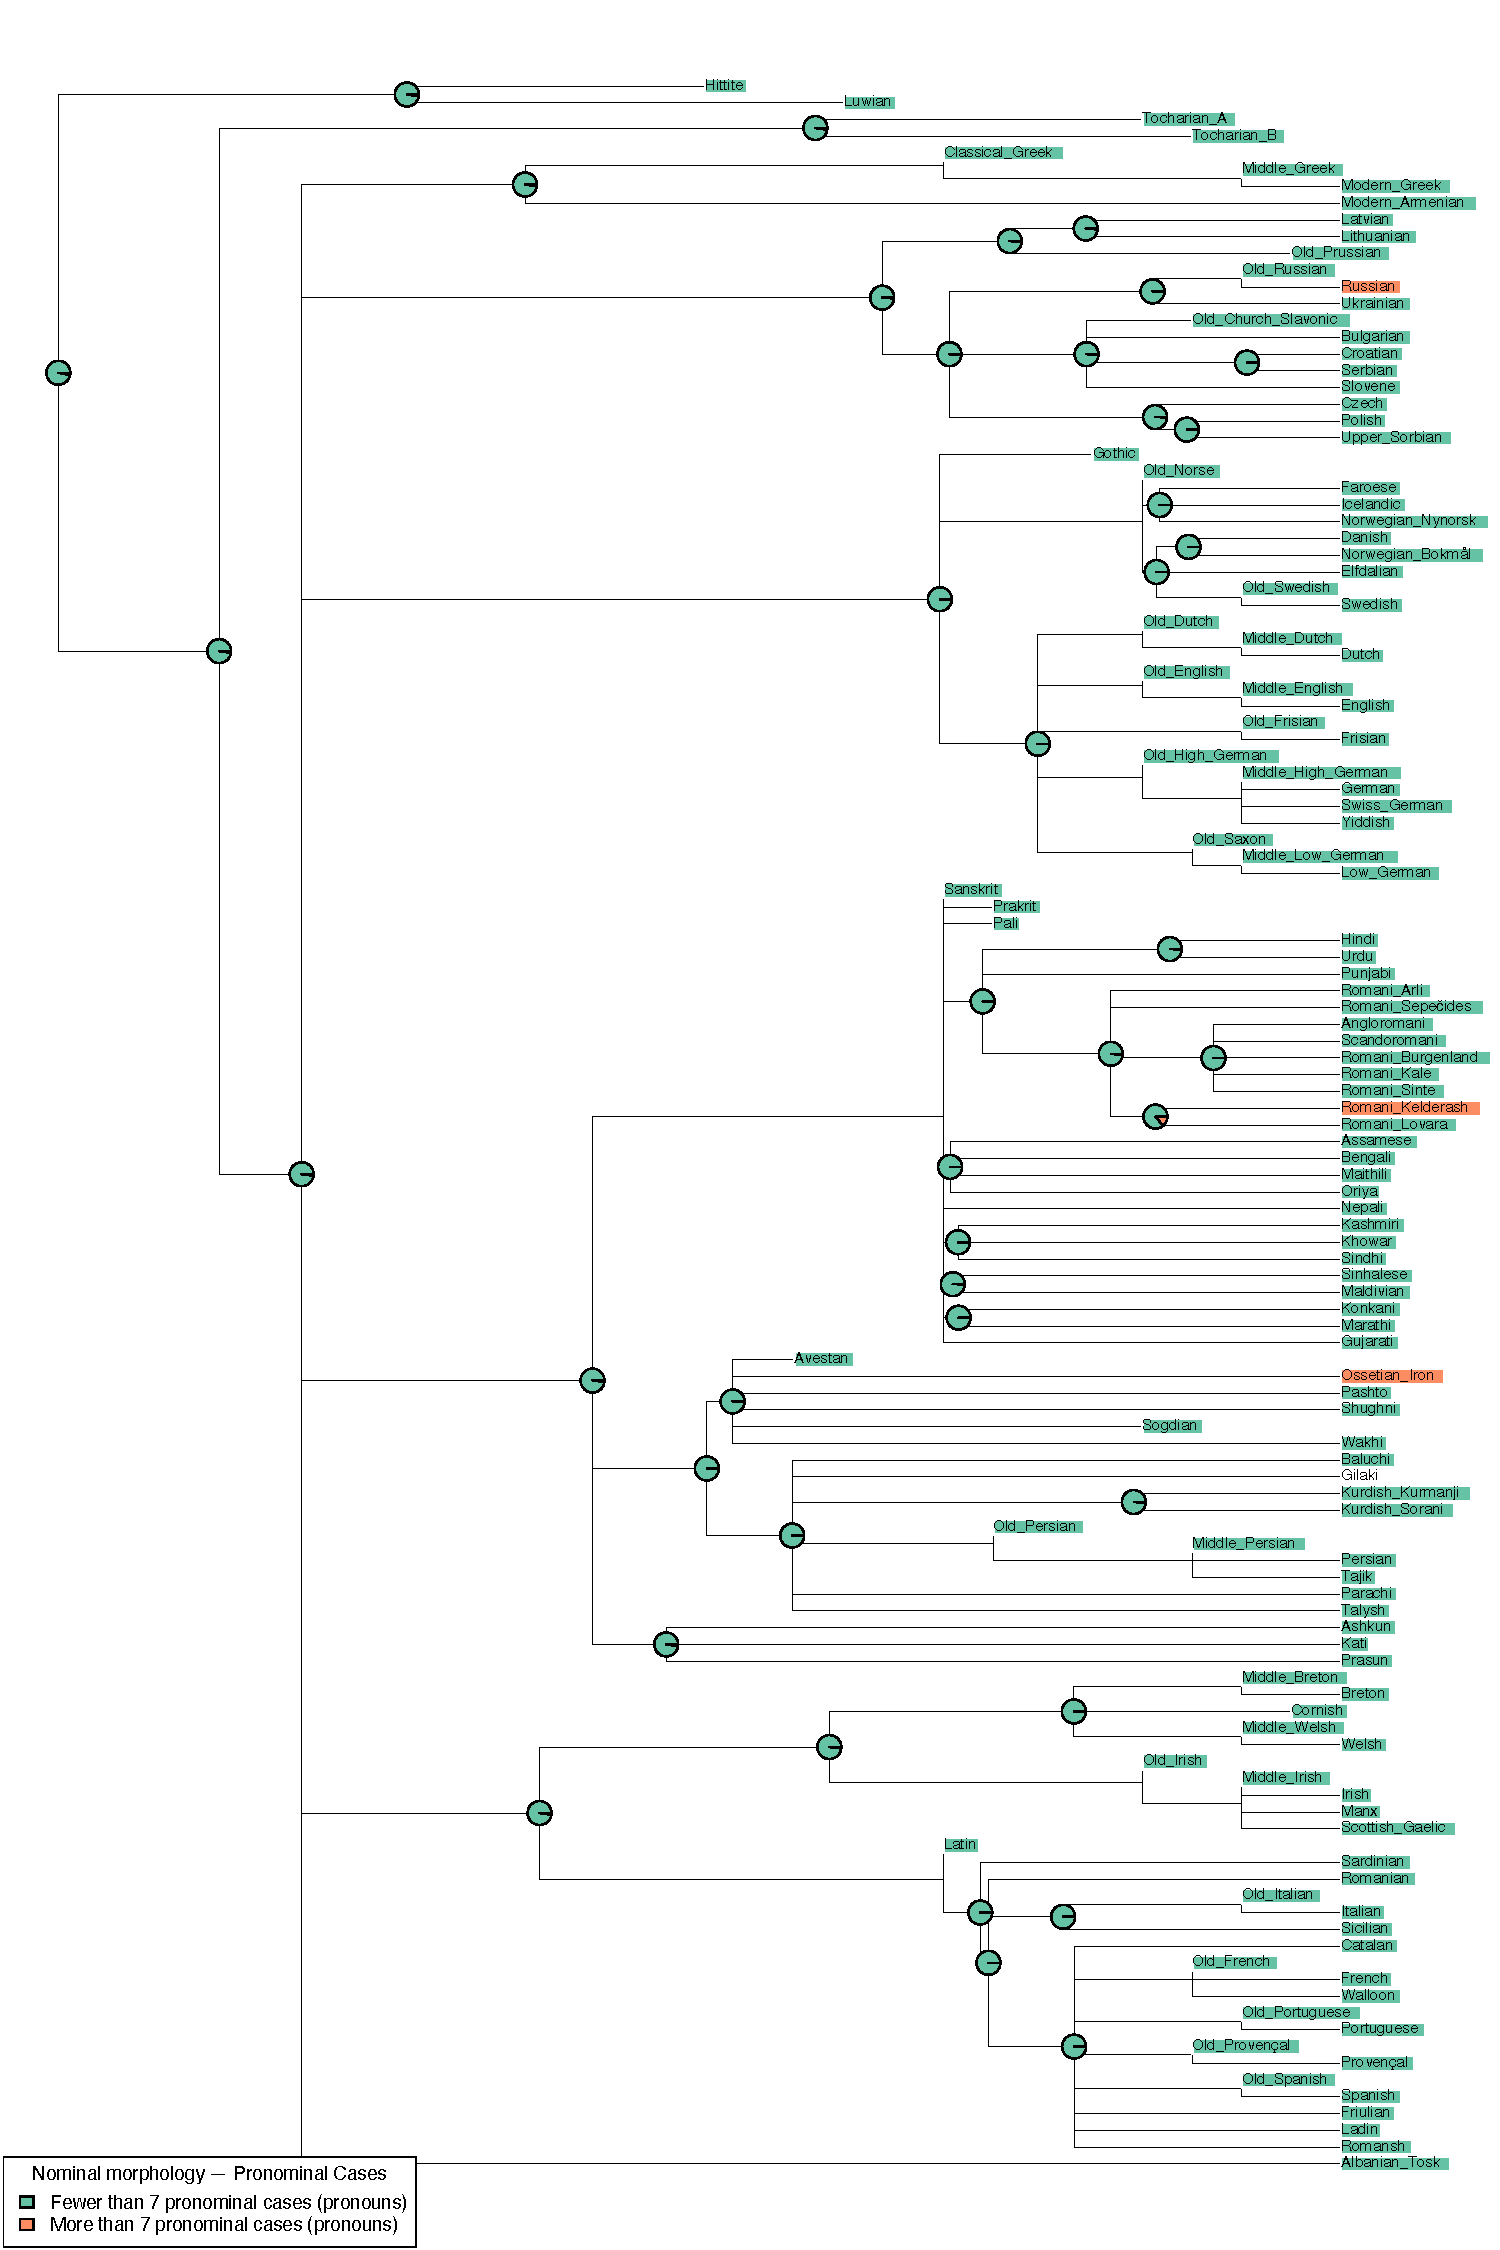
\includegraphics[width=.9\linewidth]{supp-graphics/NominalmorphologyPronominalCases7Cases.pdf}

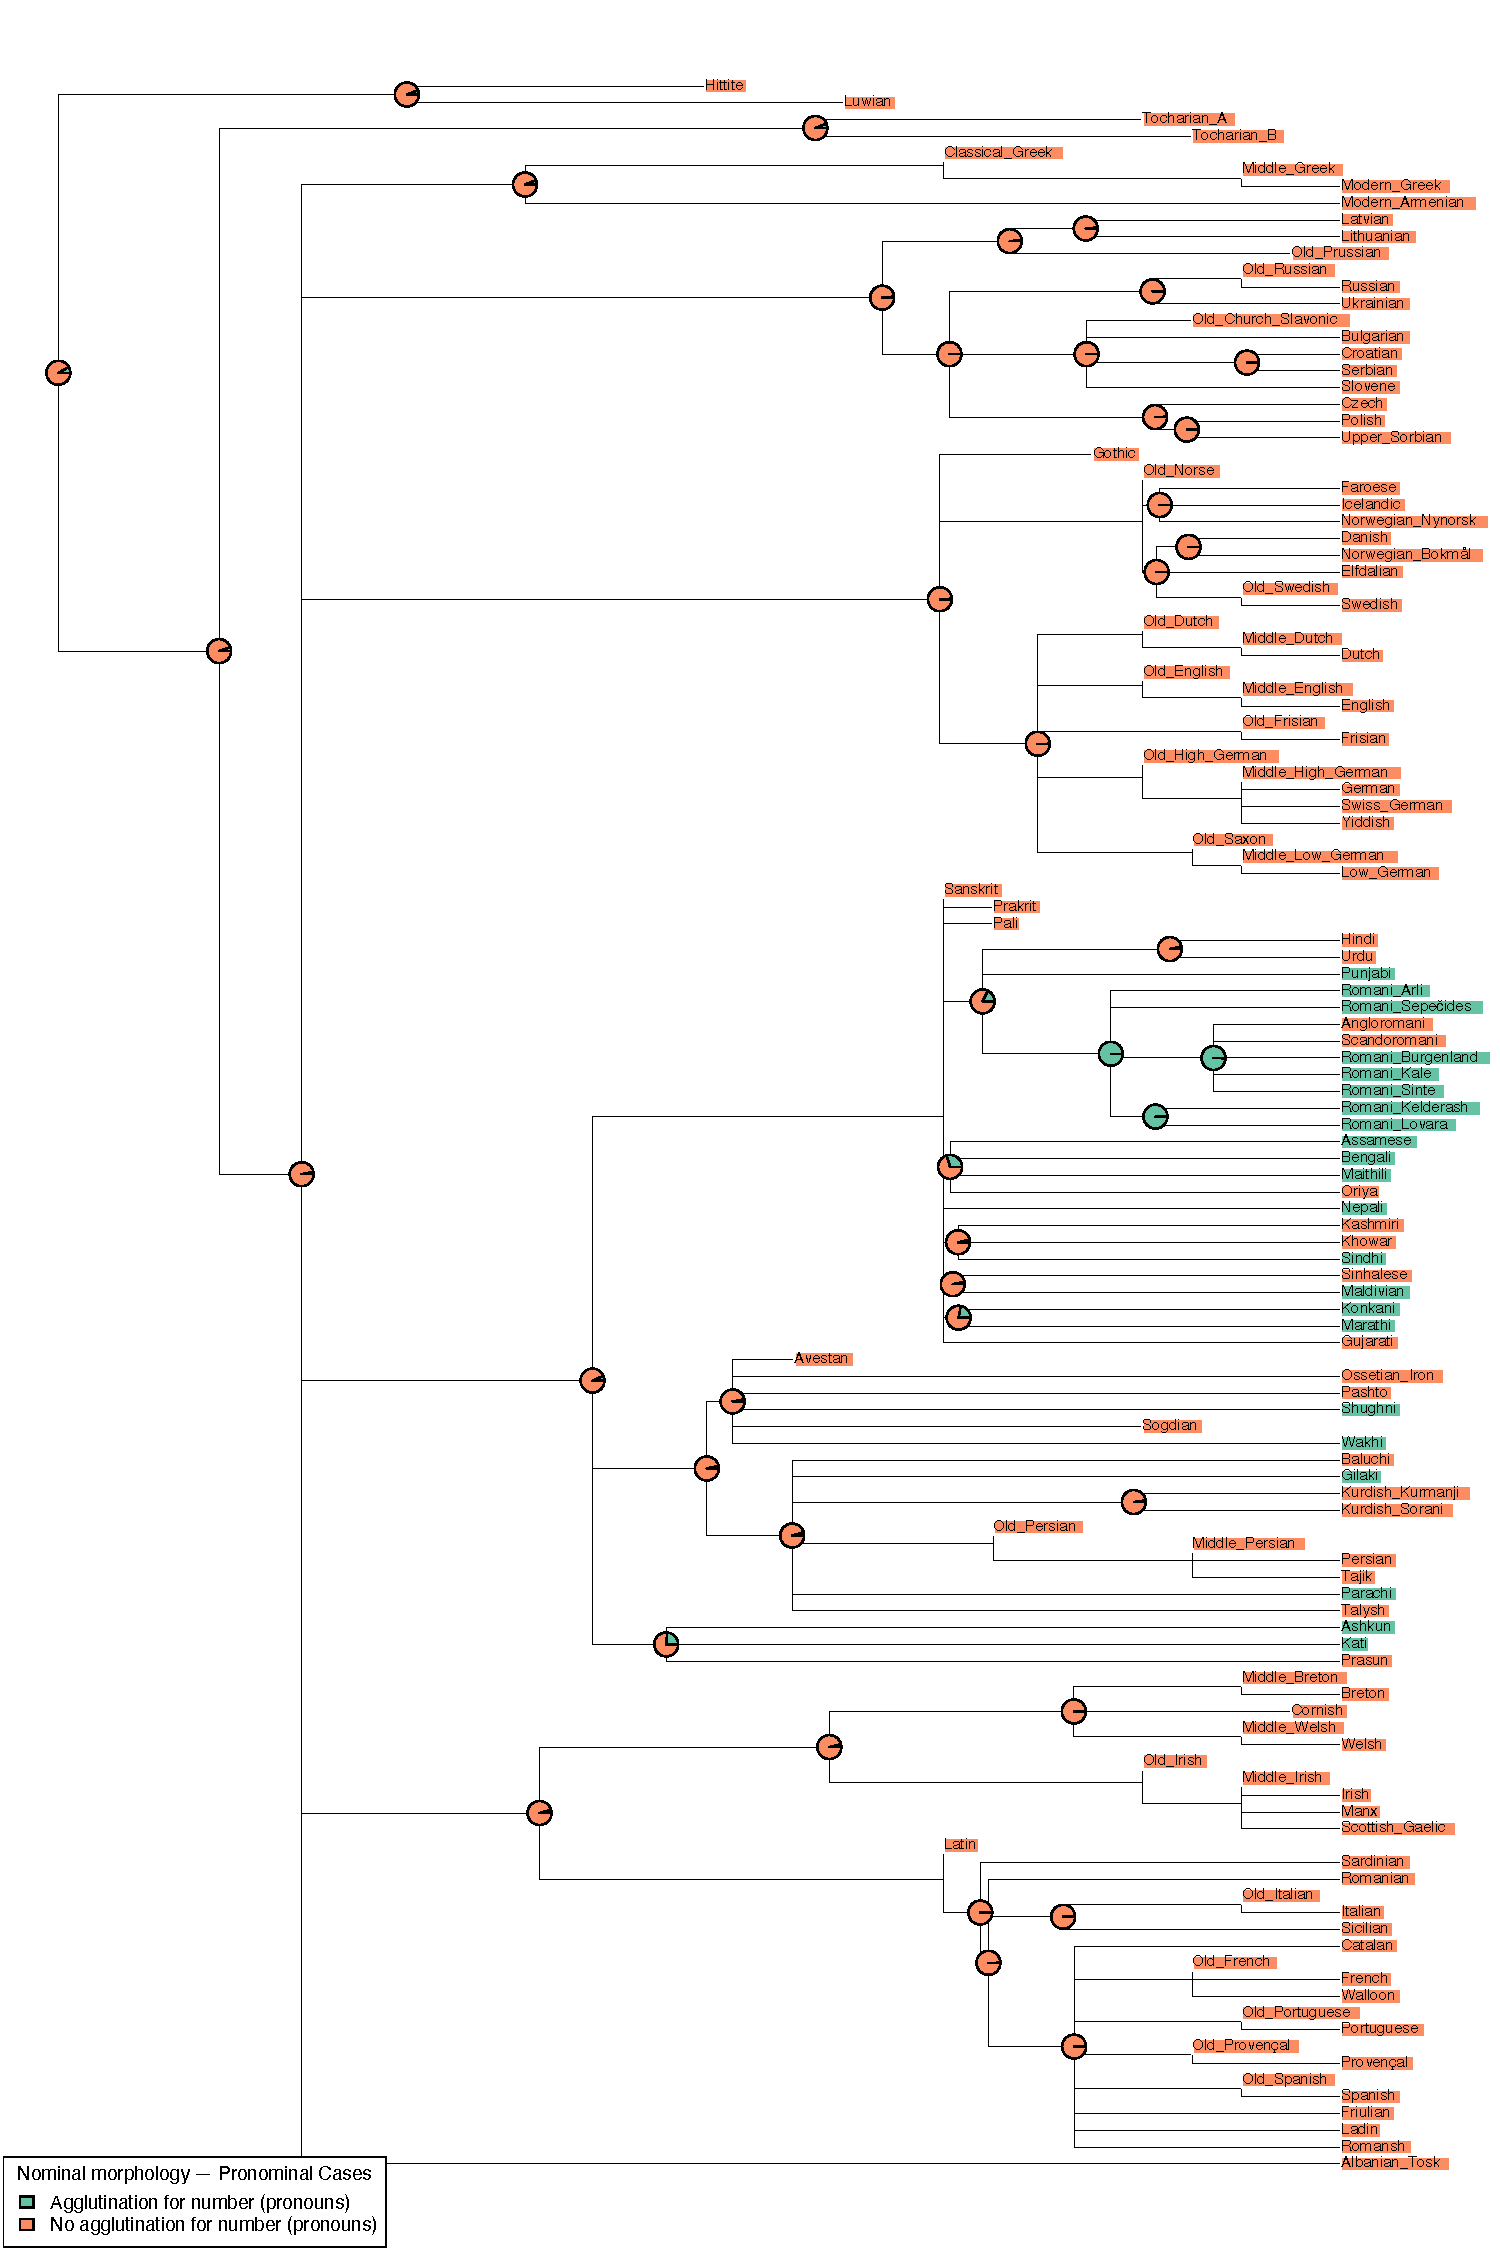
\includegraphics[width=.9\linewidth]{supp-graphics/NominalmorphologyPronominalCasesAGGLCASE.pdf}

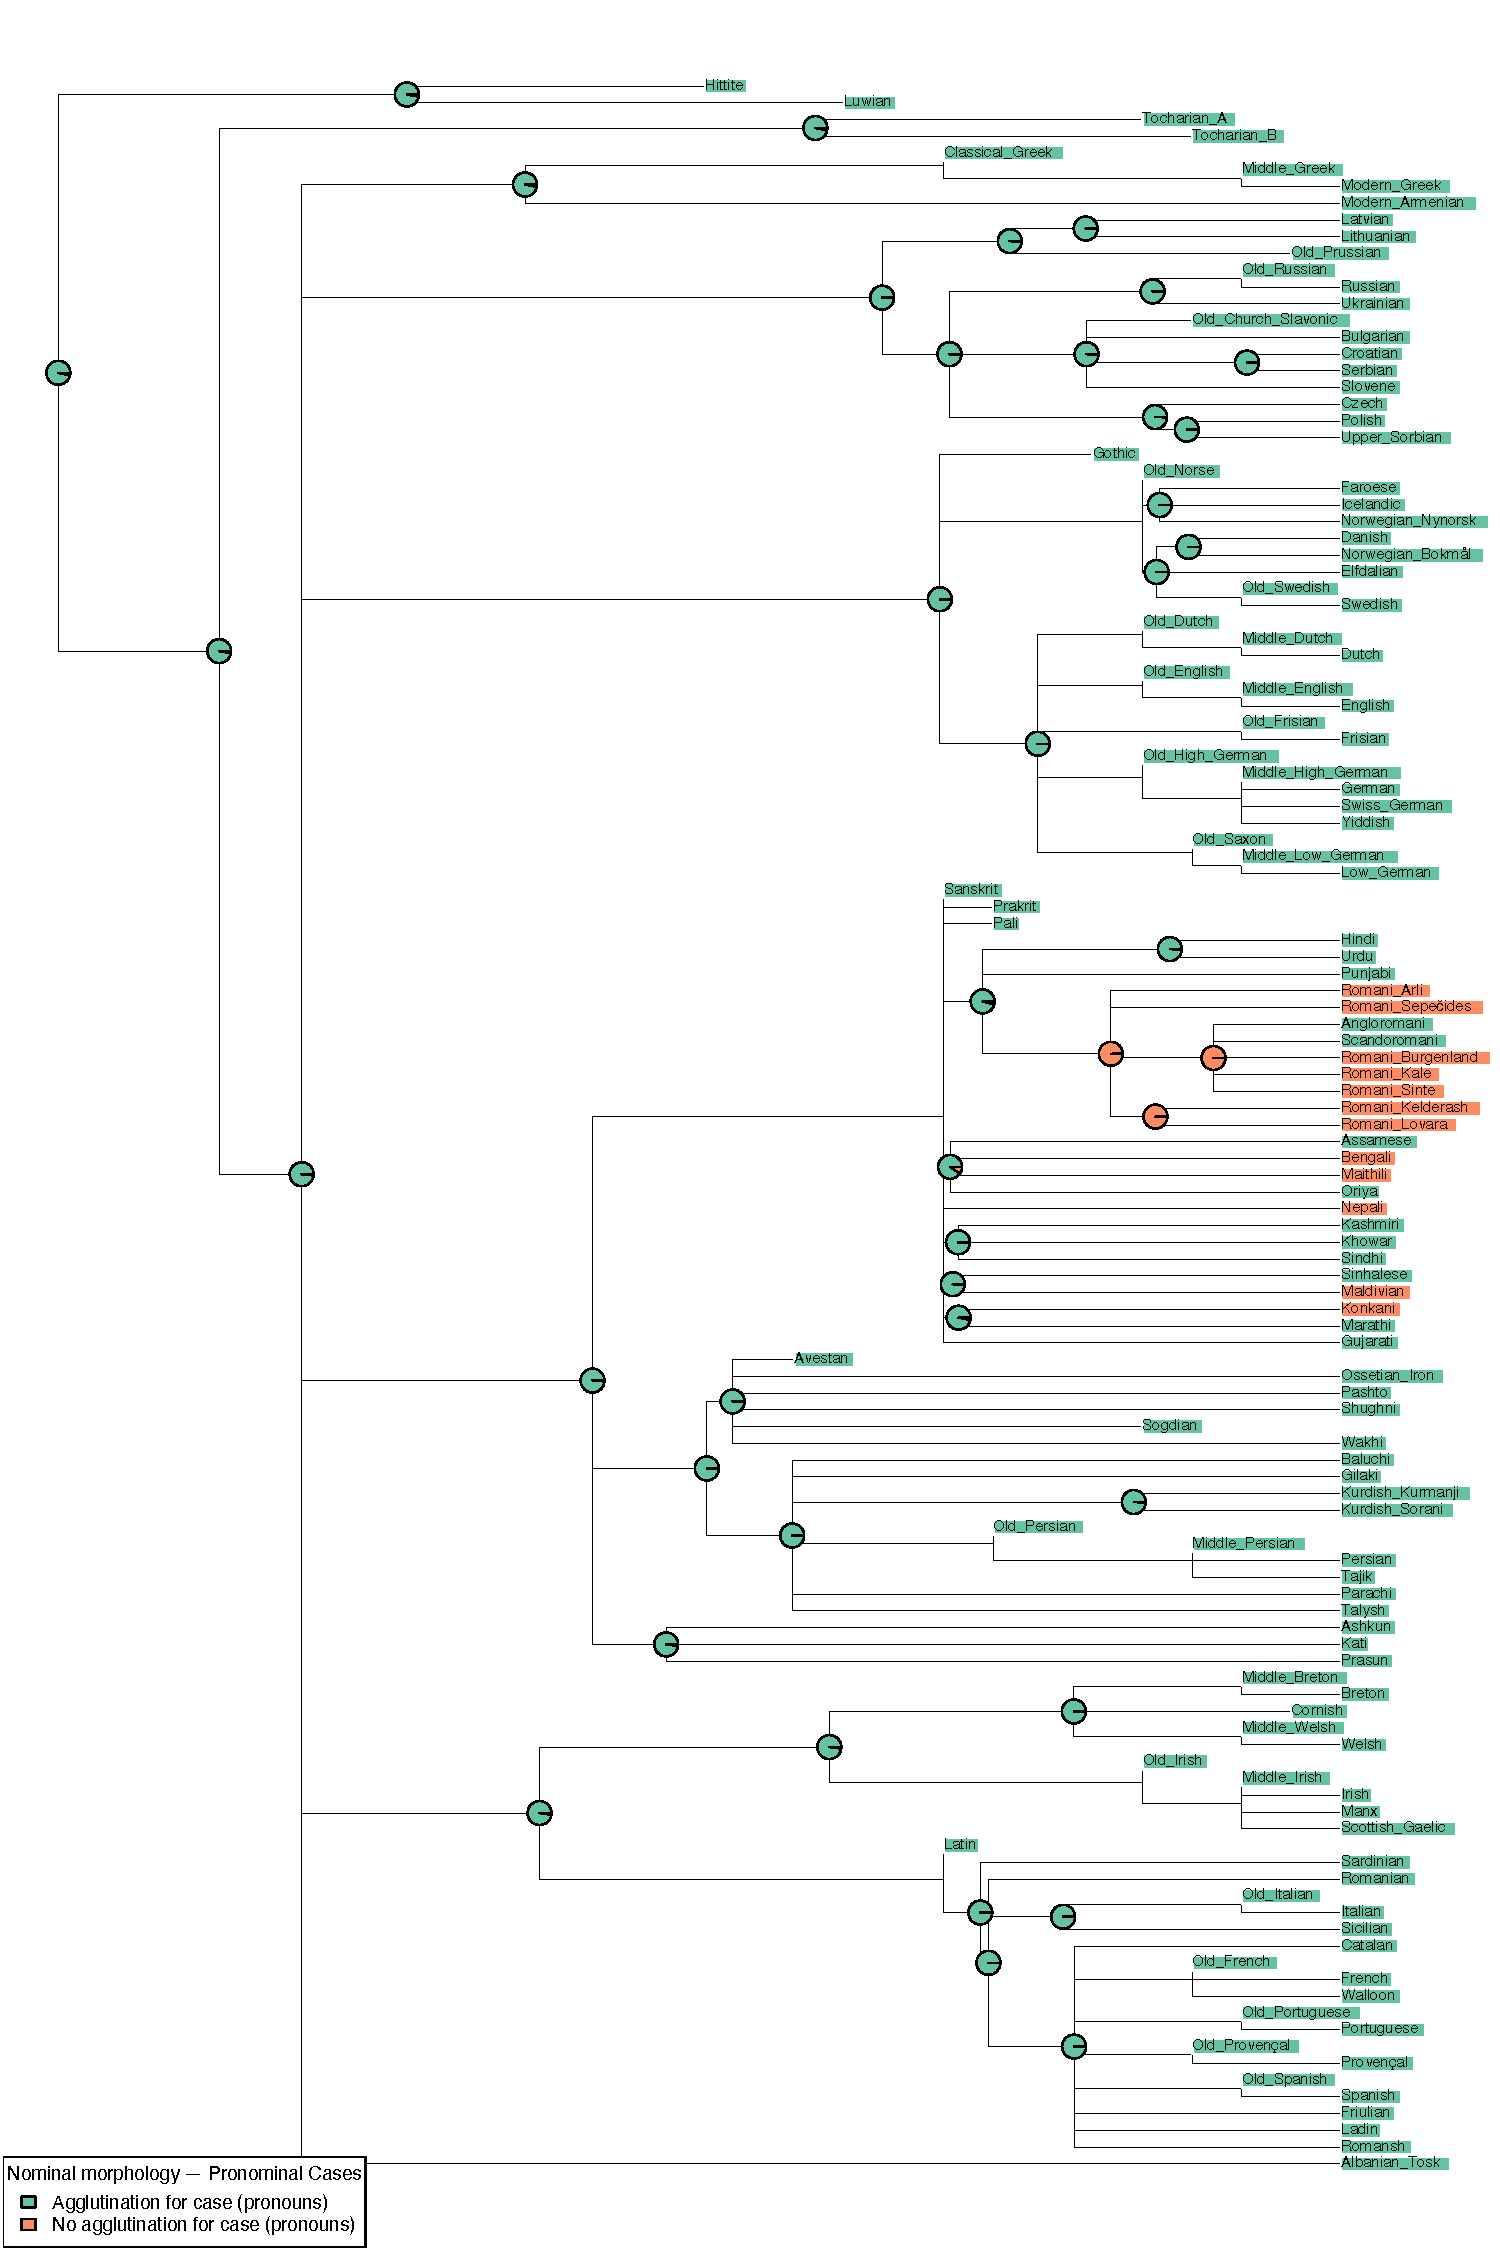
\includegraphics[width=.9\linewidth]{supp-graphics/NominalmorphologyPronominalCasesAGGLCASENR.pdf}

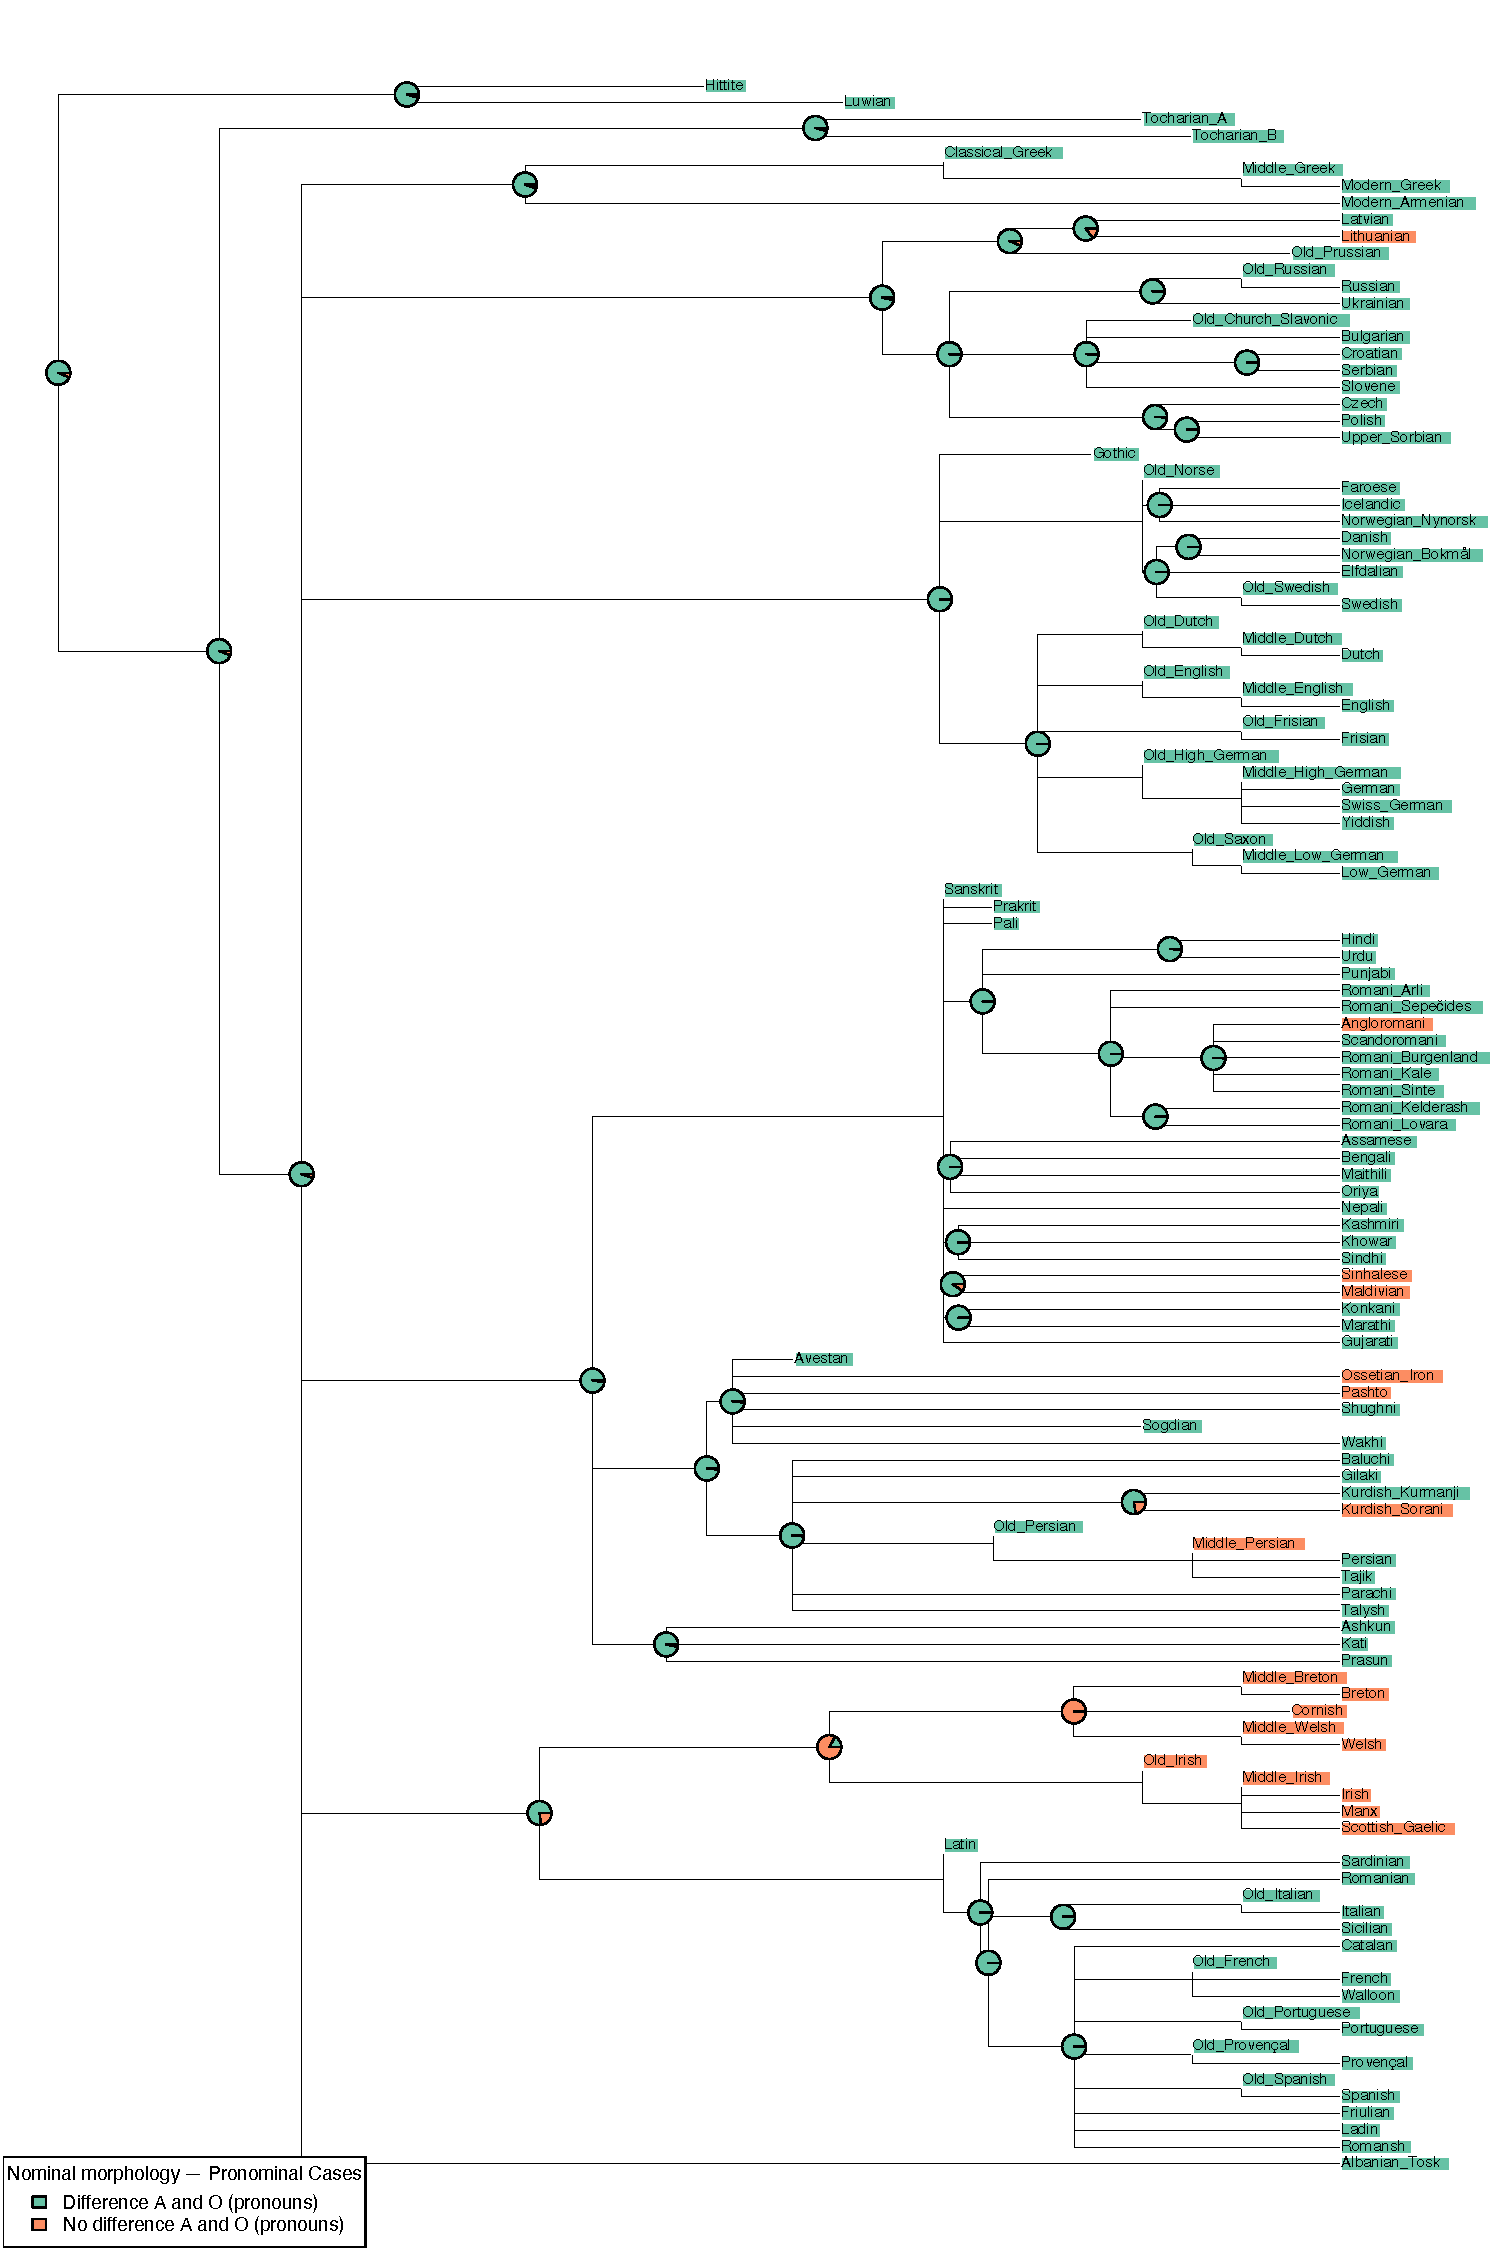
\includegraphics[width=.9\linewidth]{supp-graphics/NominalmorphologyPronominalCasesAO.pdf}

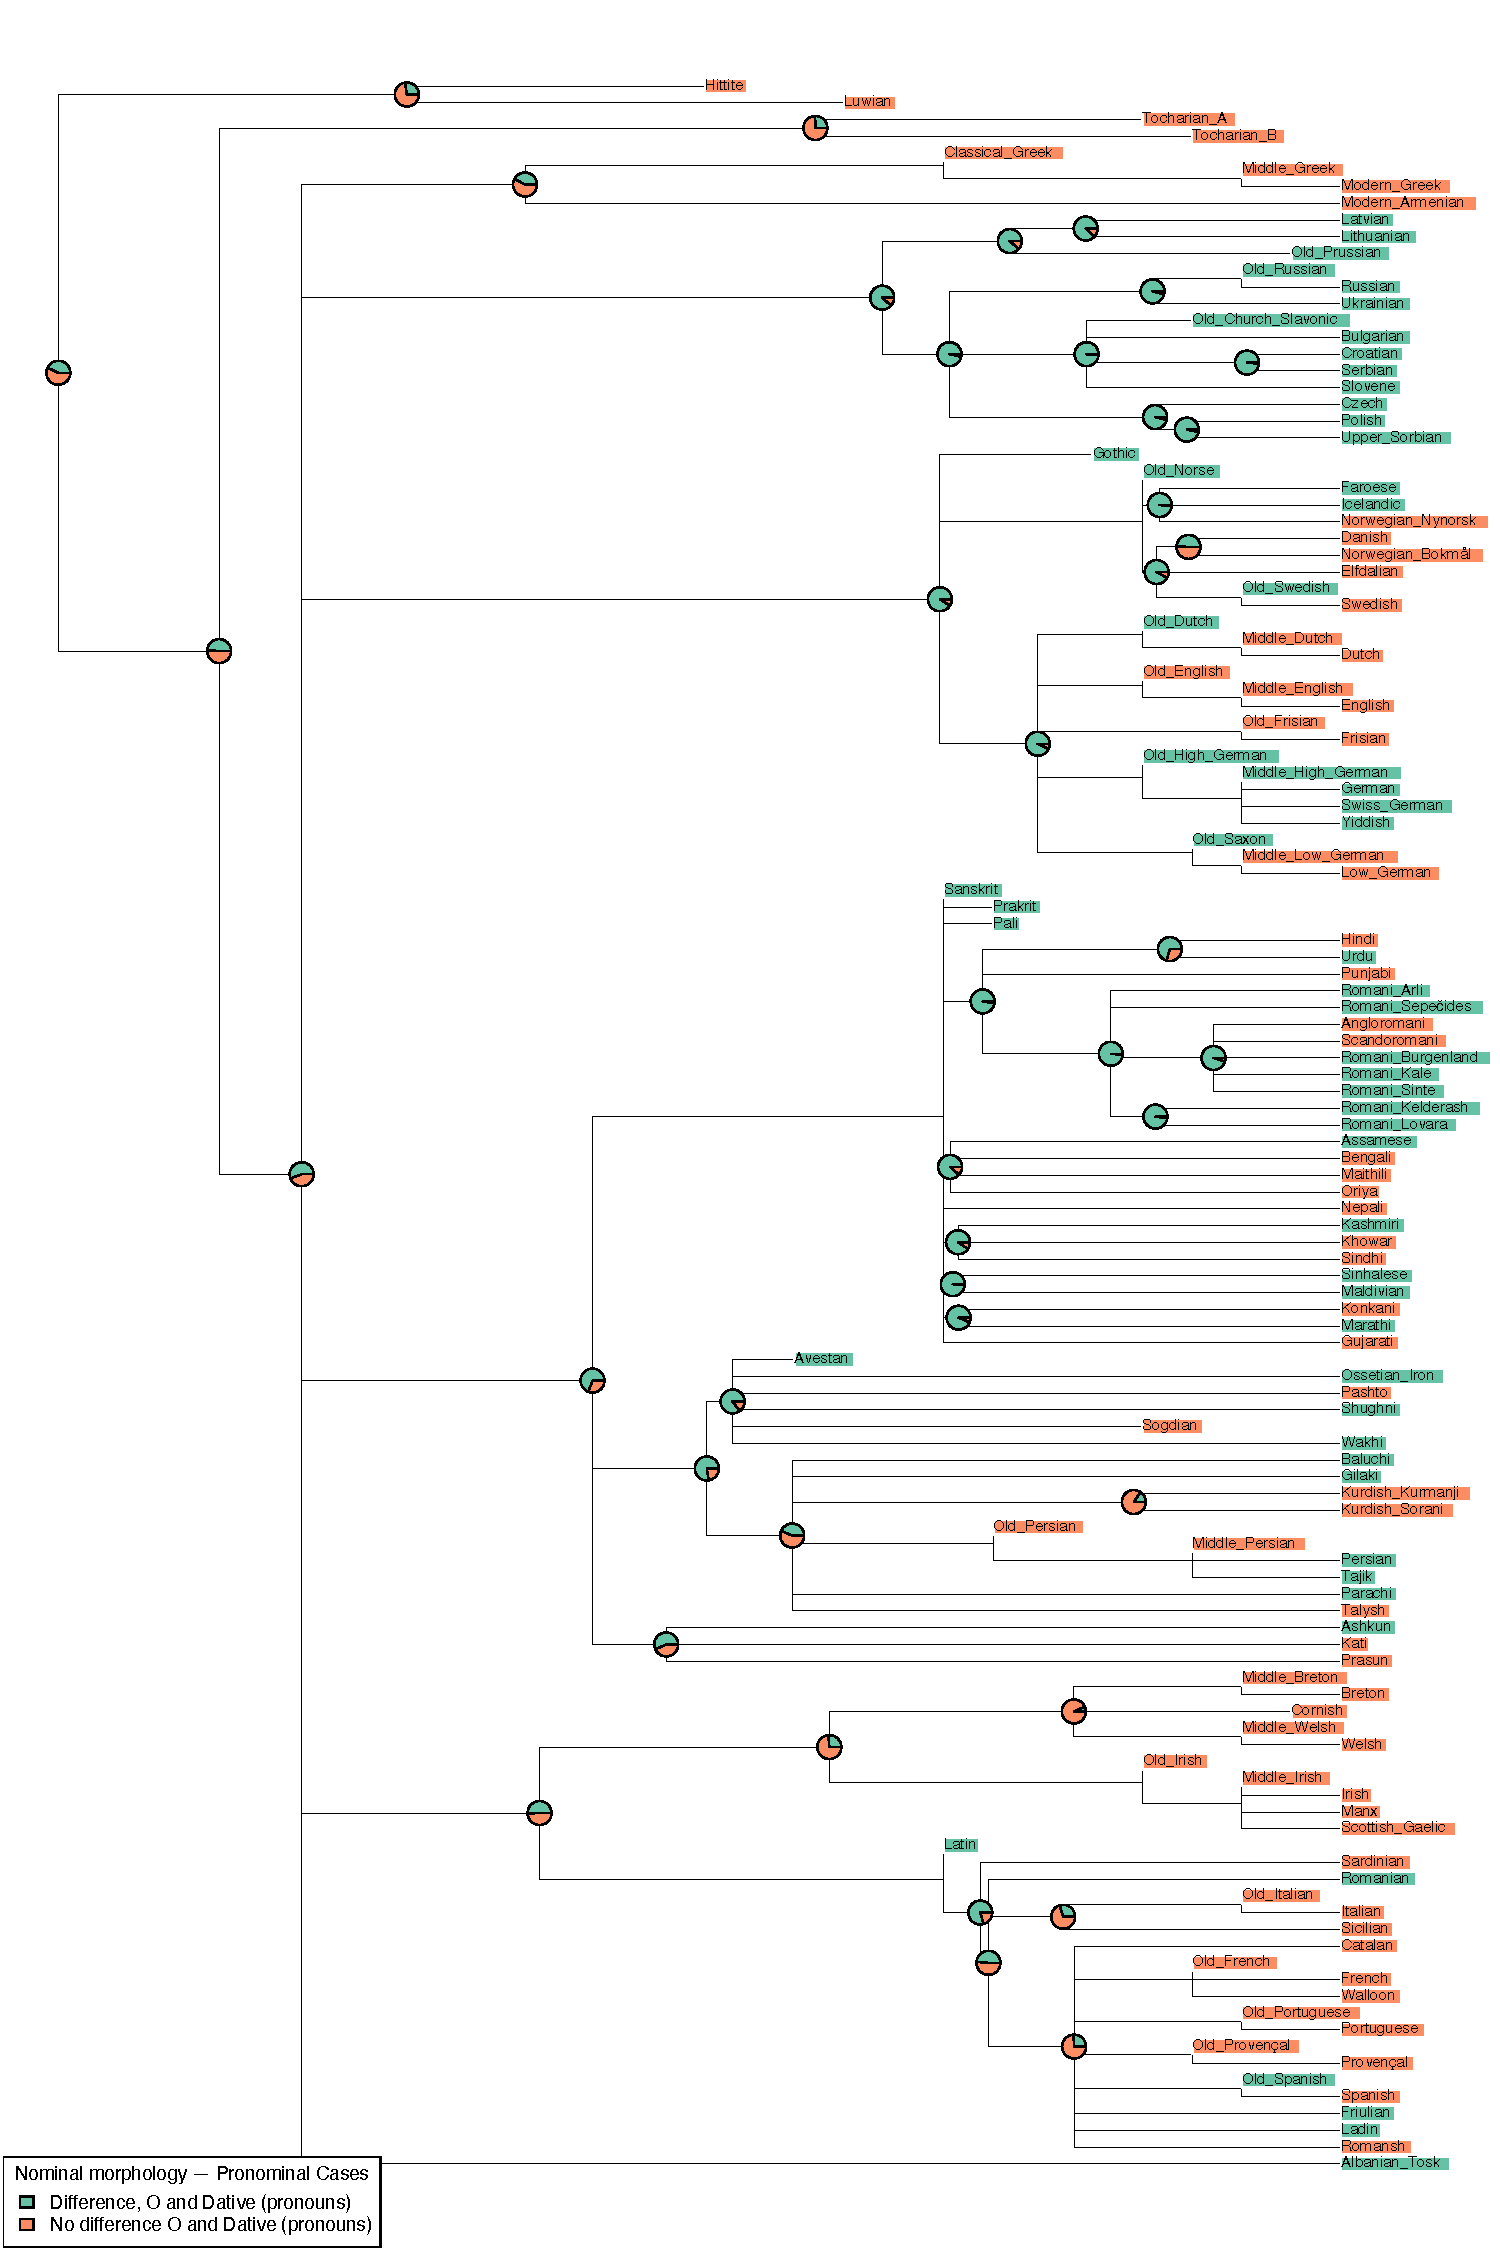
\includegraphics[width=.9\linewidth]{supp-graphics/NominalmorphologyPronominalCasesDATO.pdf}

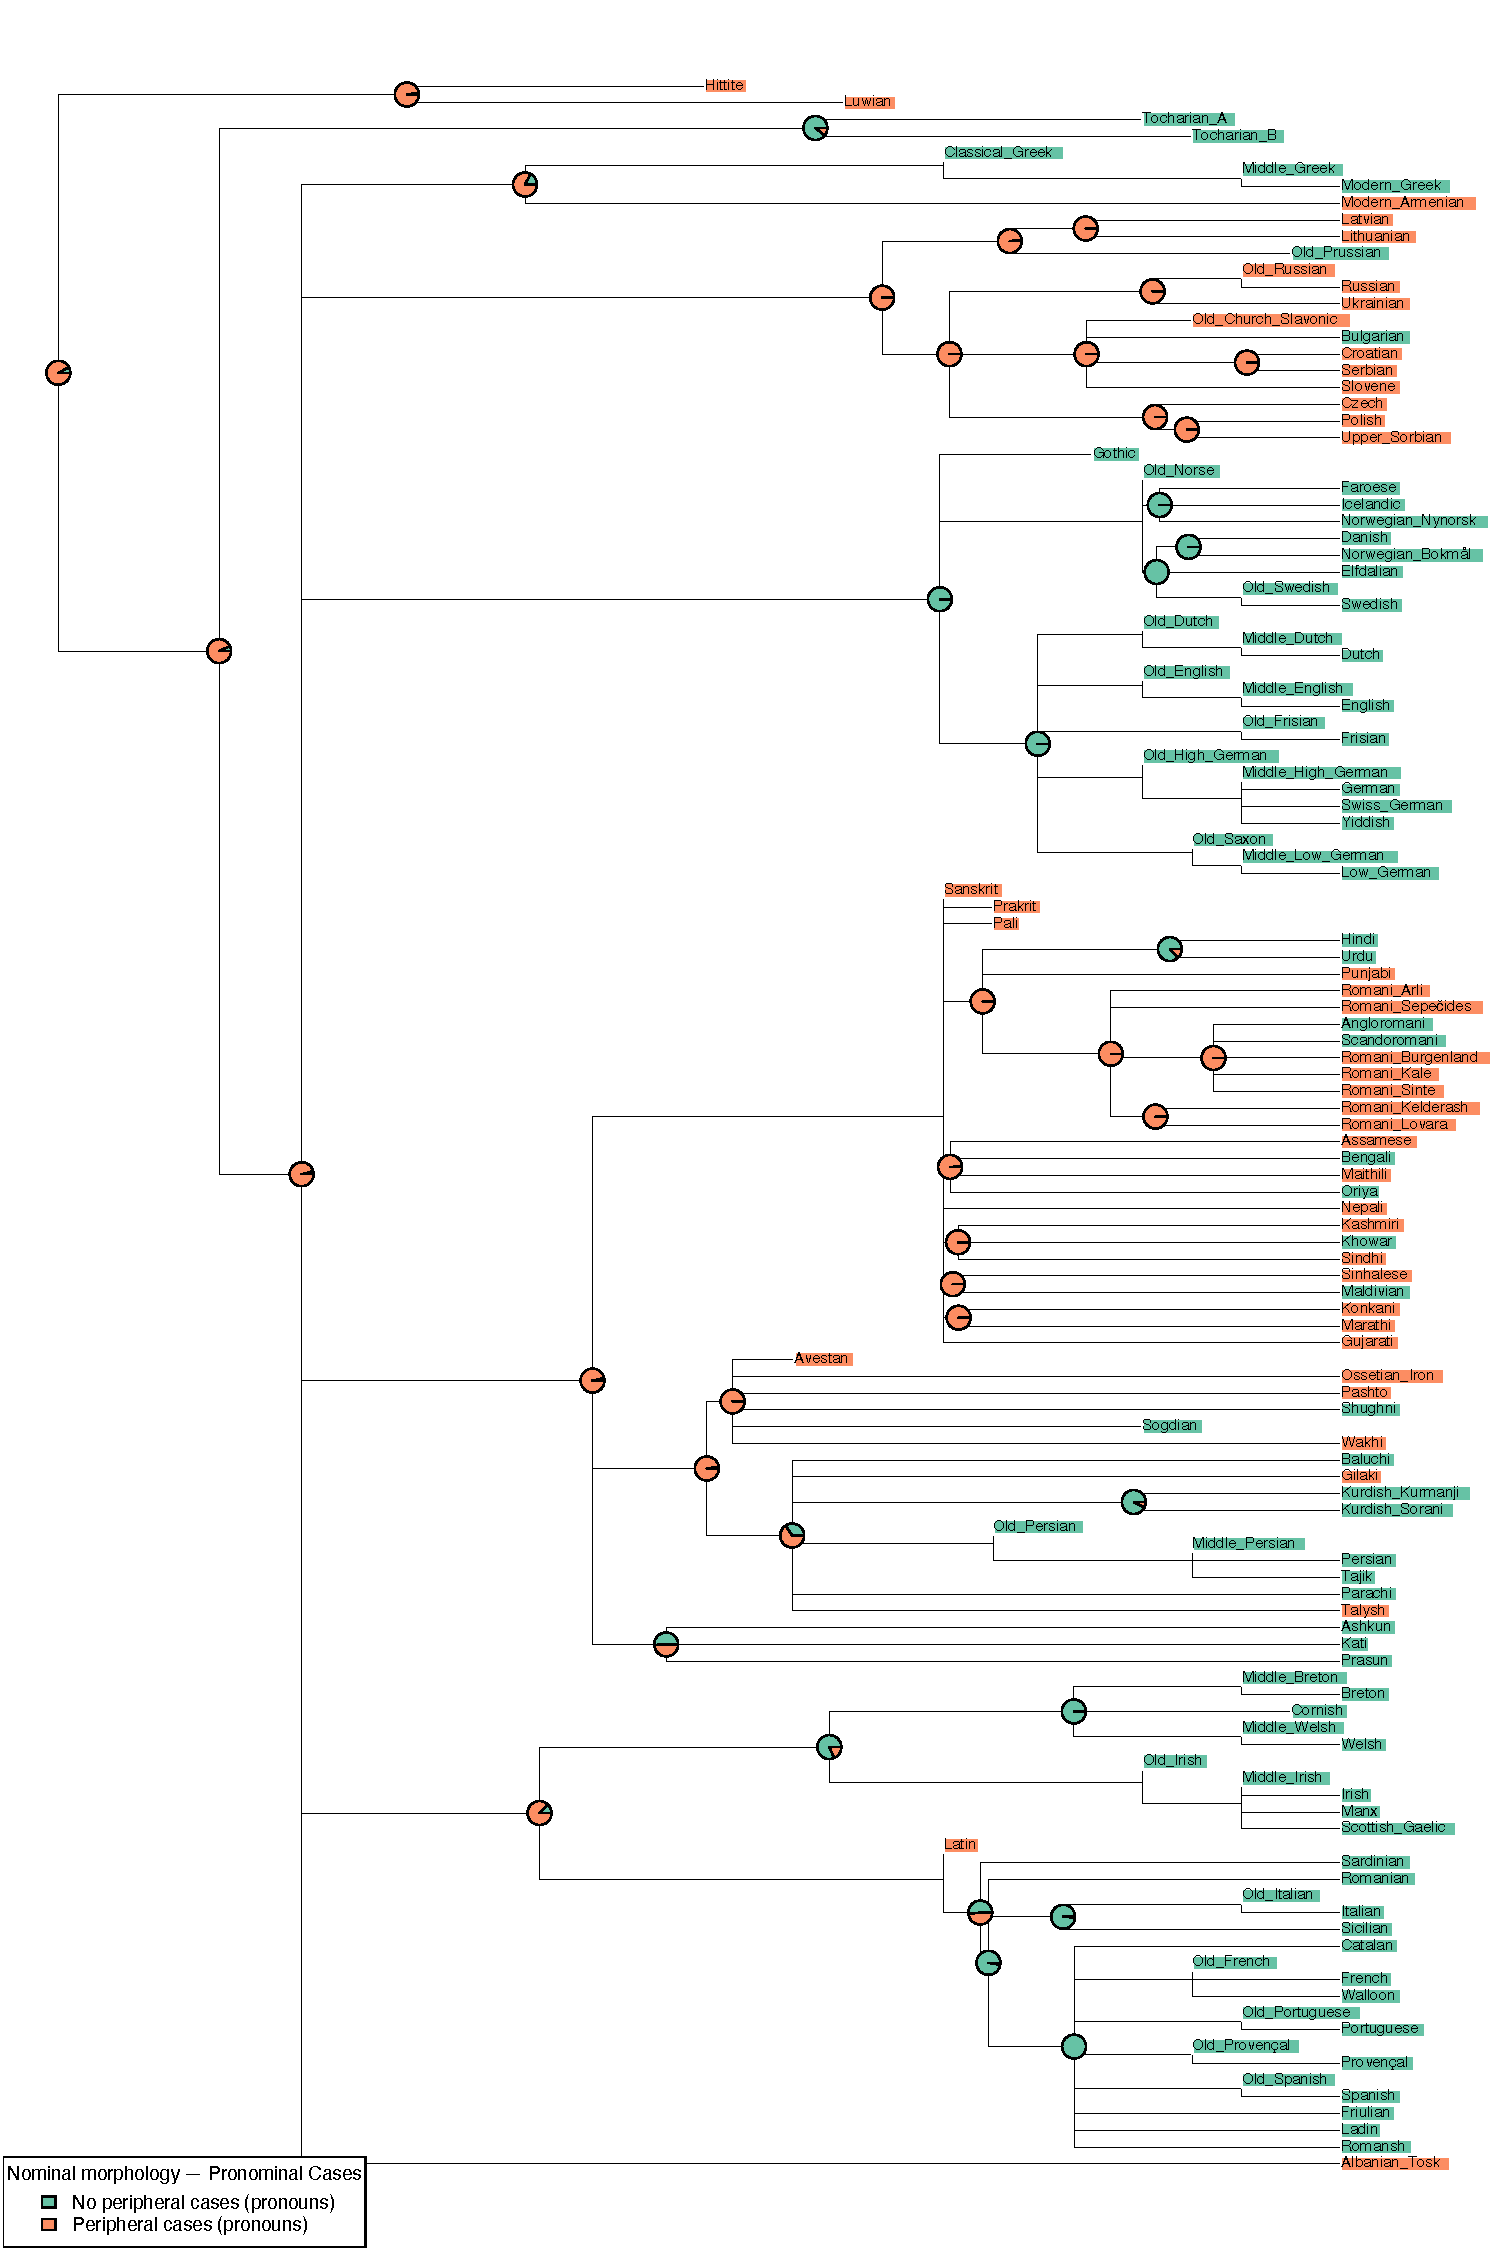
\includegraphics[width=.9\linewidth]{supp-graphics/NominalmorphologyPronominalCasesOBLCases.pdf}

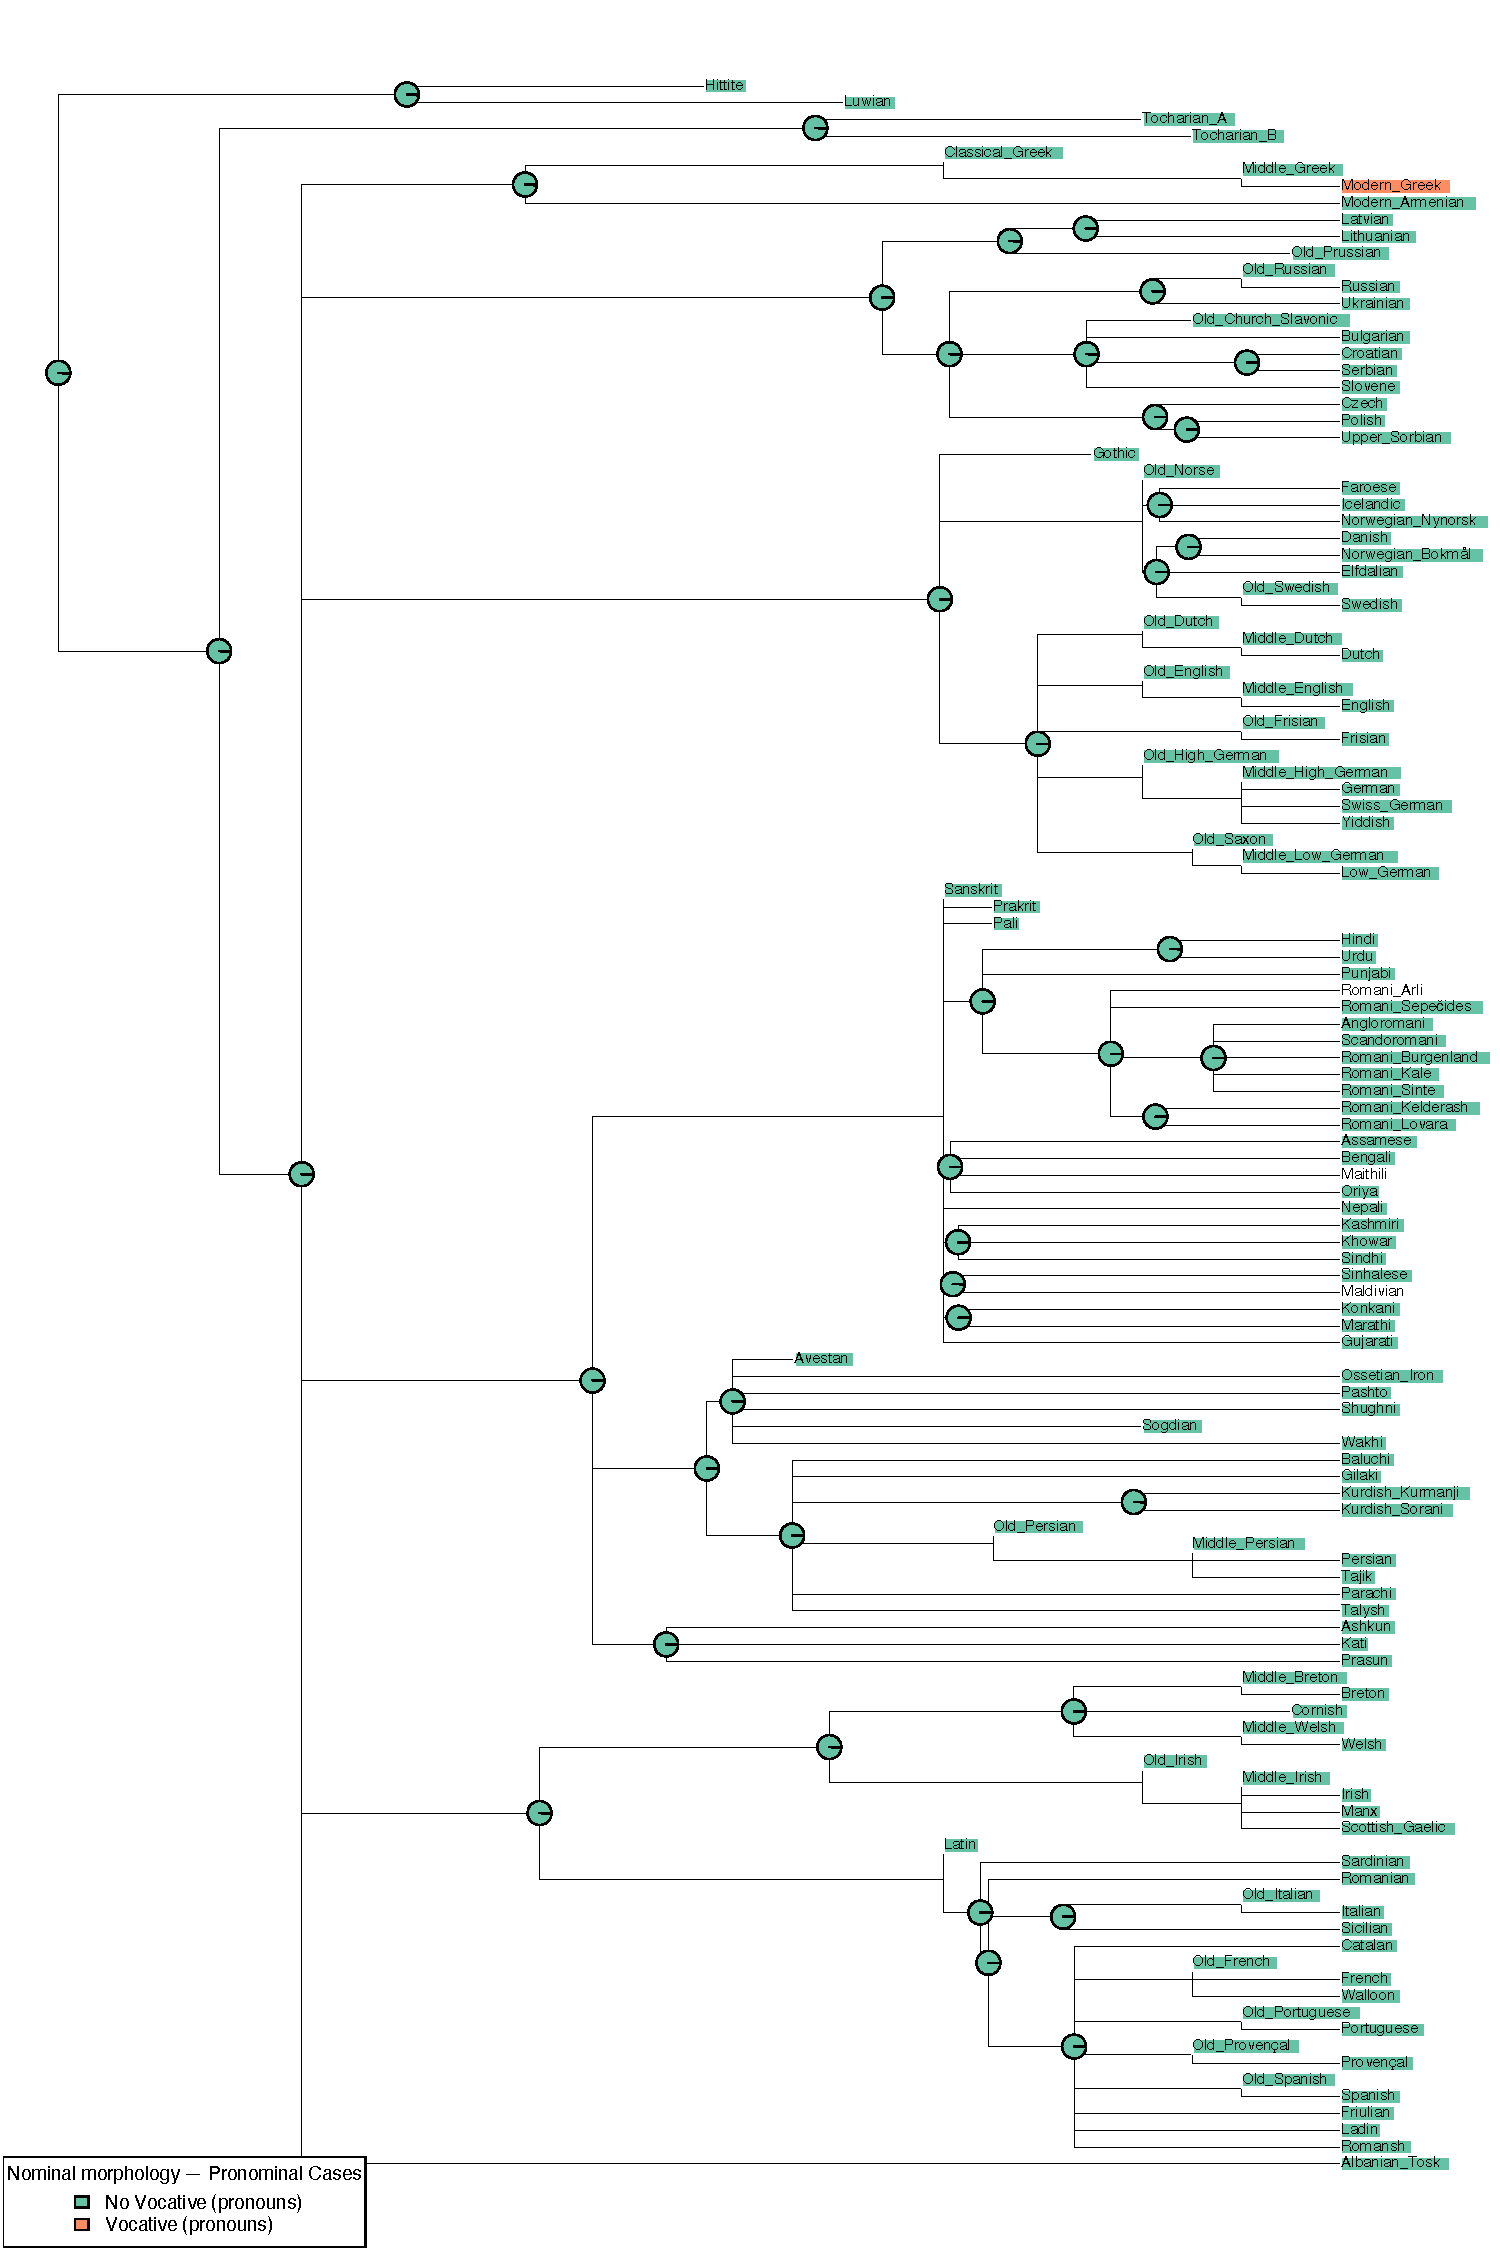
\includegraphics[width=.9\linewidth]{supp-graphics/NominalmorphologyPronominalCasesVOC.pdf}

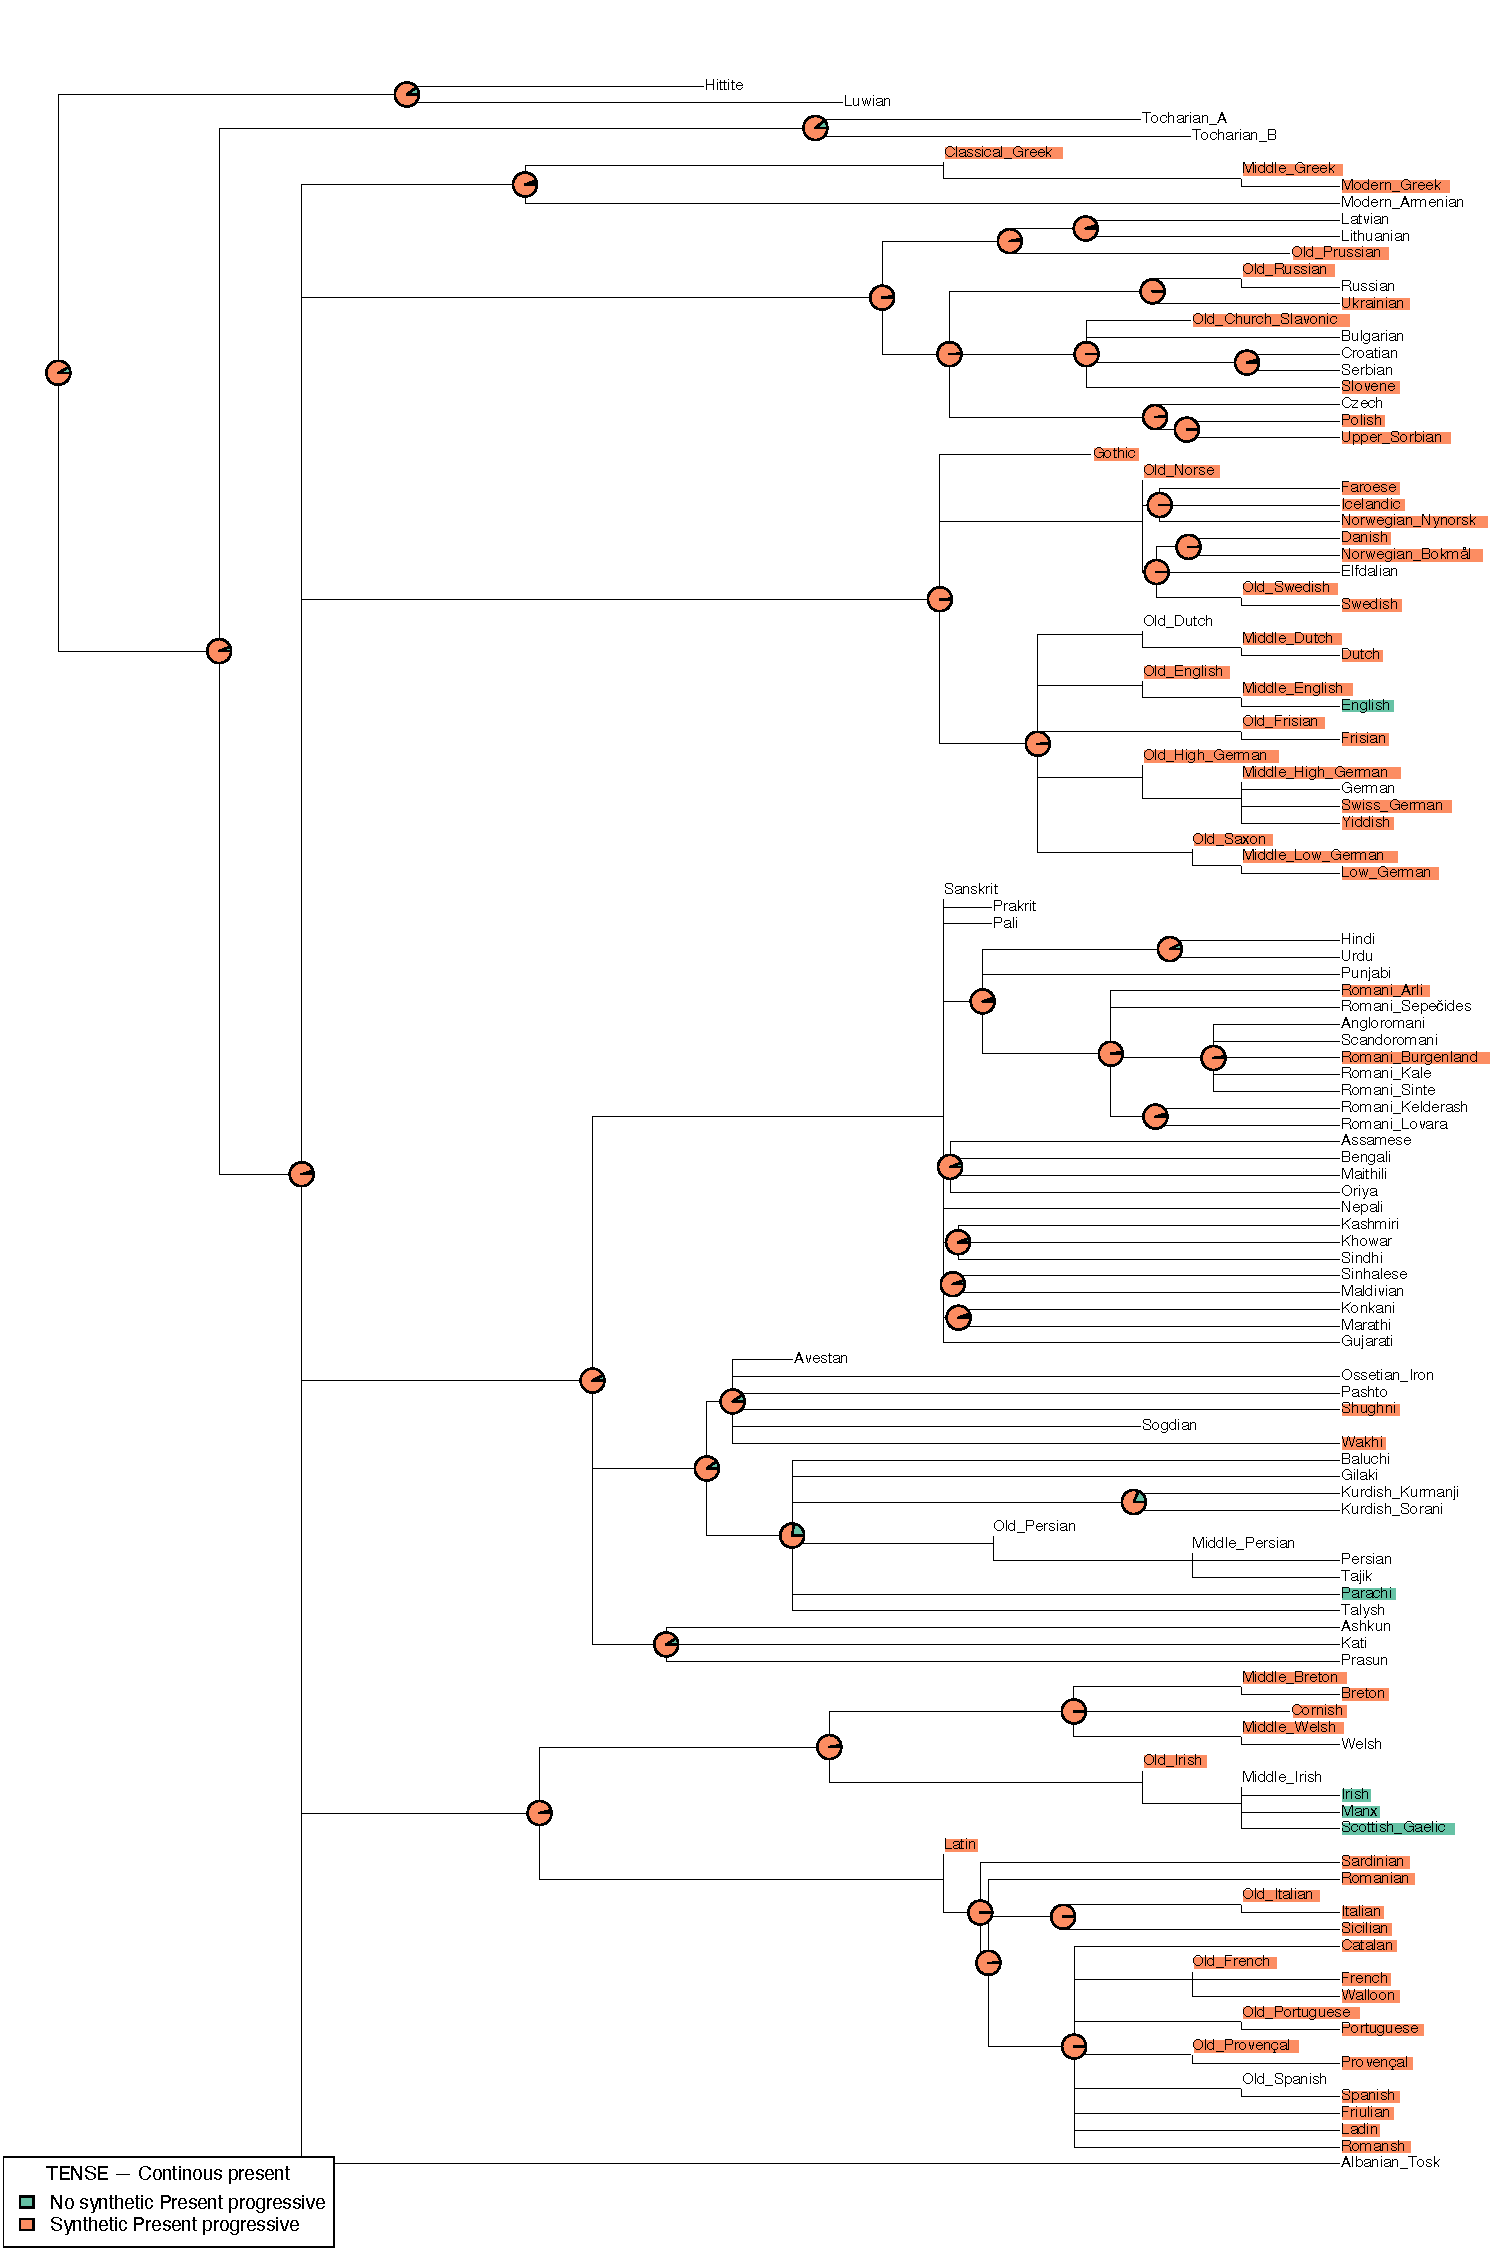
\includegraphics[width=.9\linewidth]{supp-graphics/TENSEContinouspresentPresent.pdf}

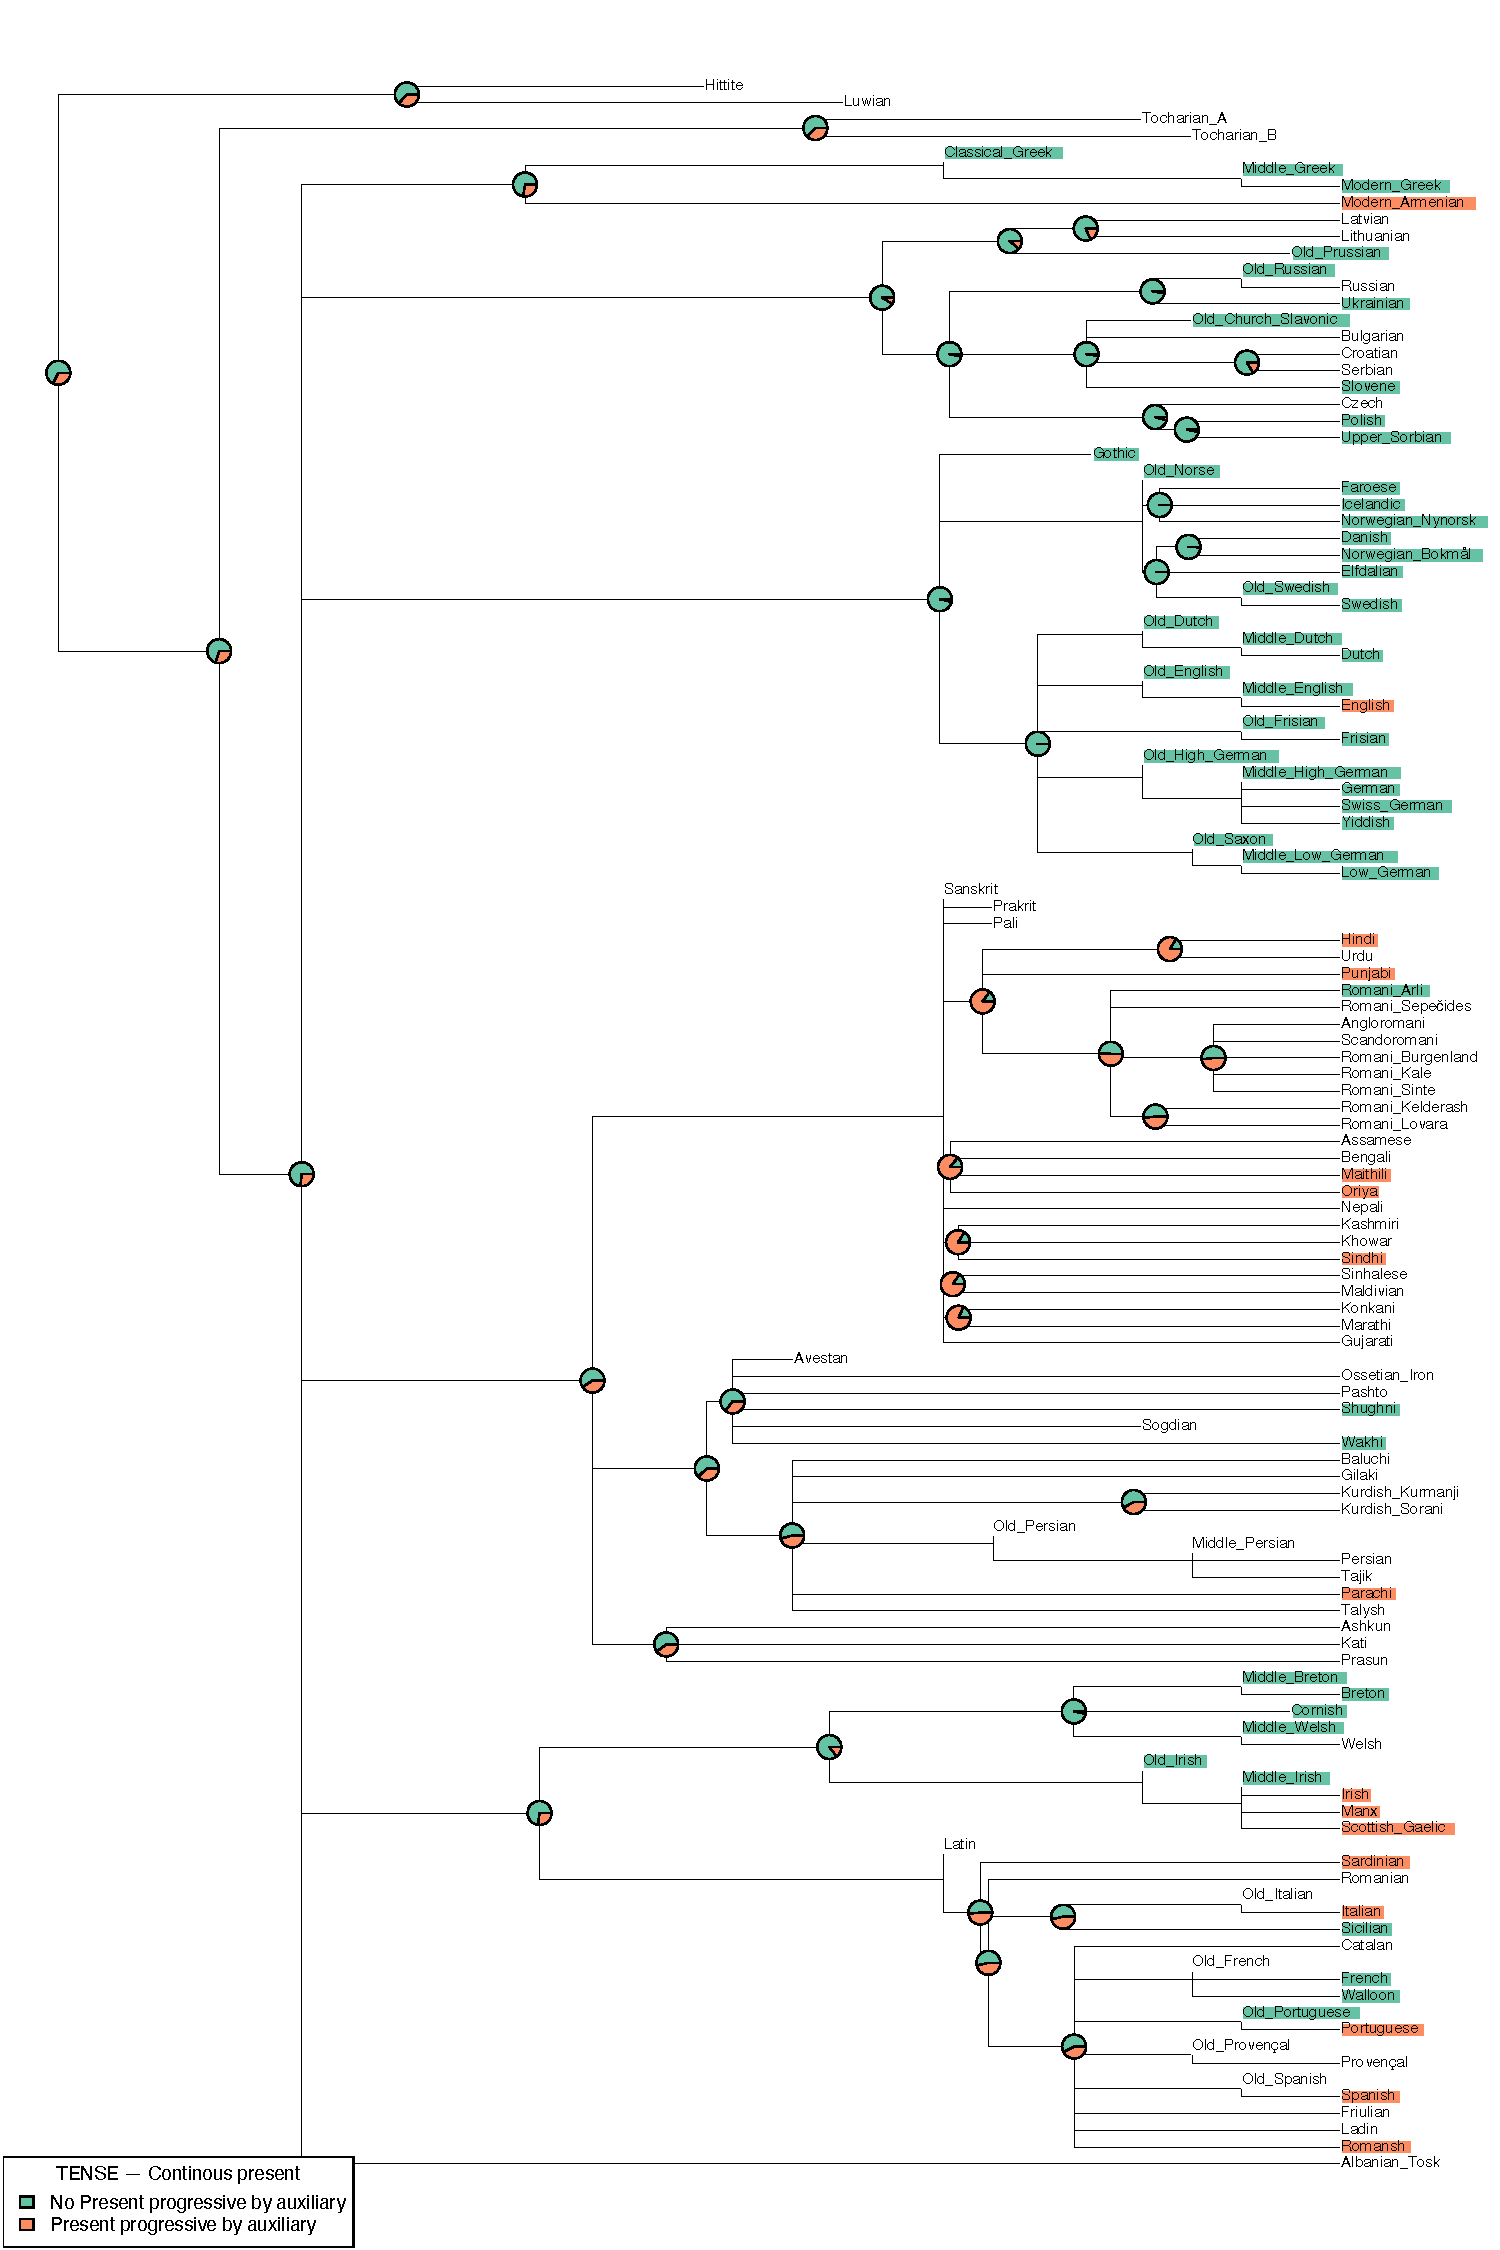
\includegraphics[width=.9\linewidth]{supp-graphics/TENSEContinouspresentProgressivepresent.pdf}

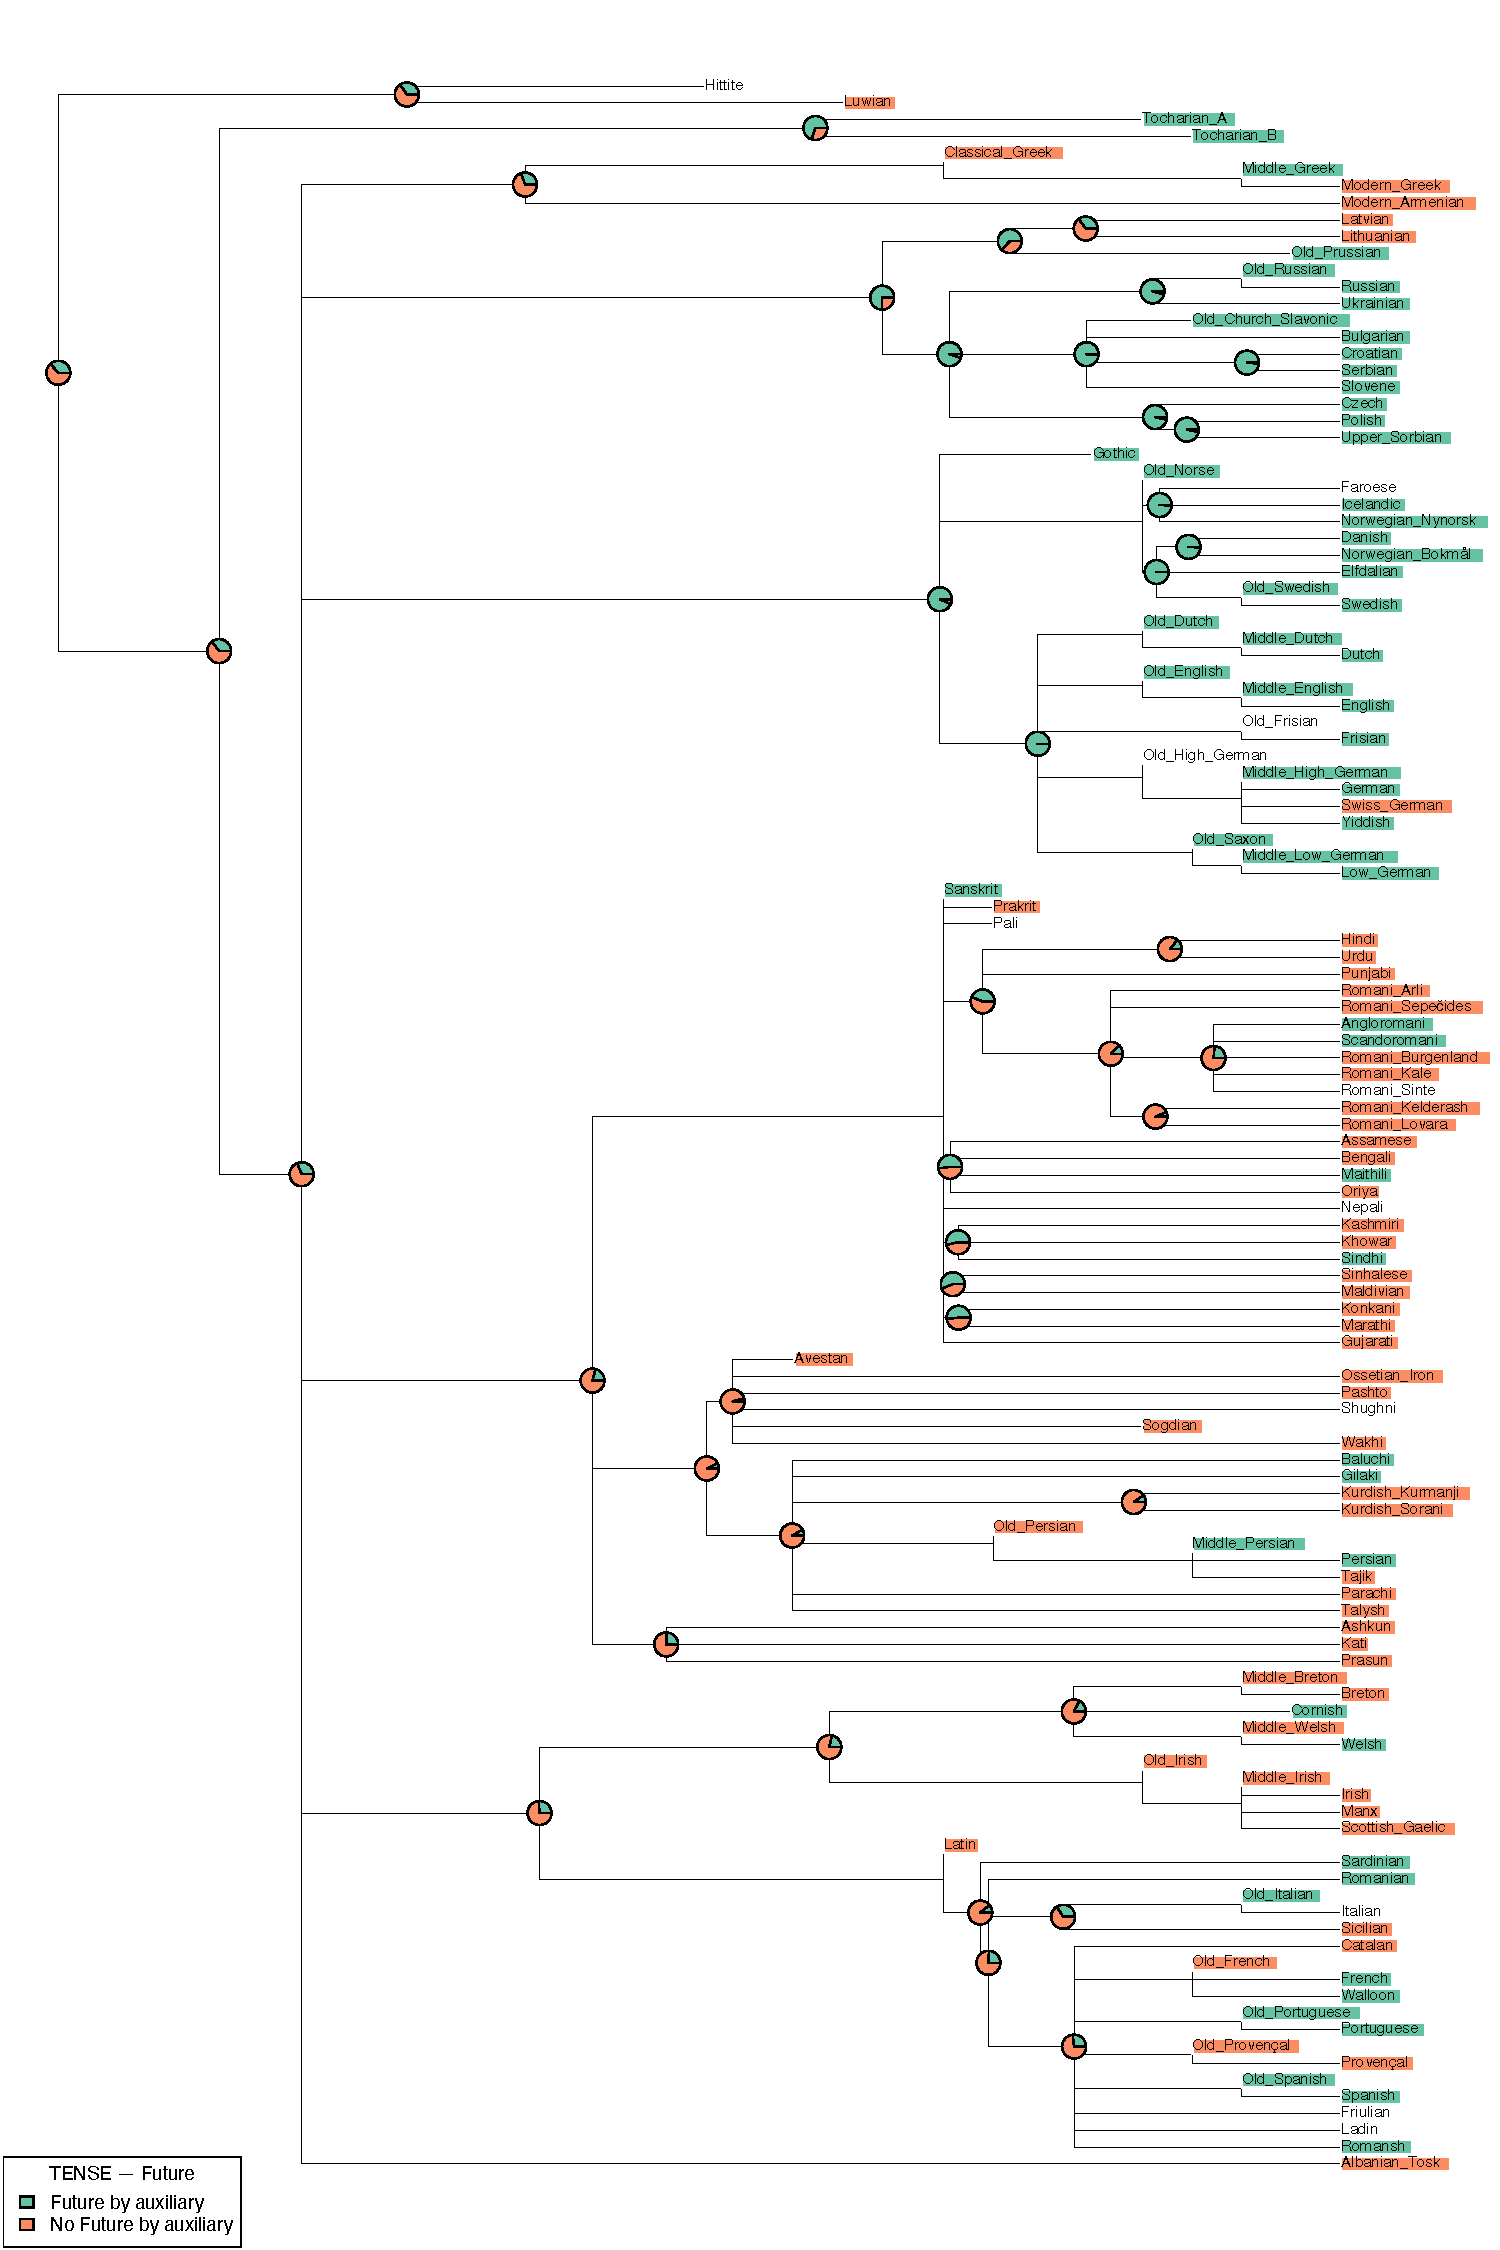
\includegraphics[width=.9\linewidth]{supp-graphics/TENSEFutureFUTAUX.pdf}

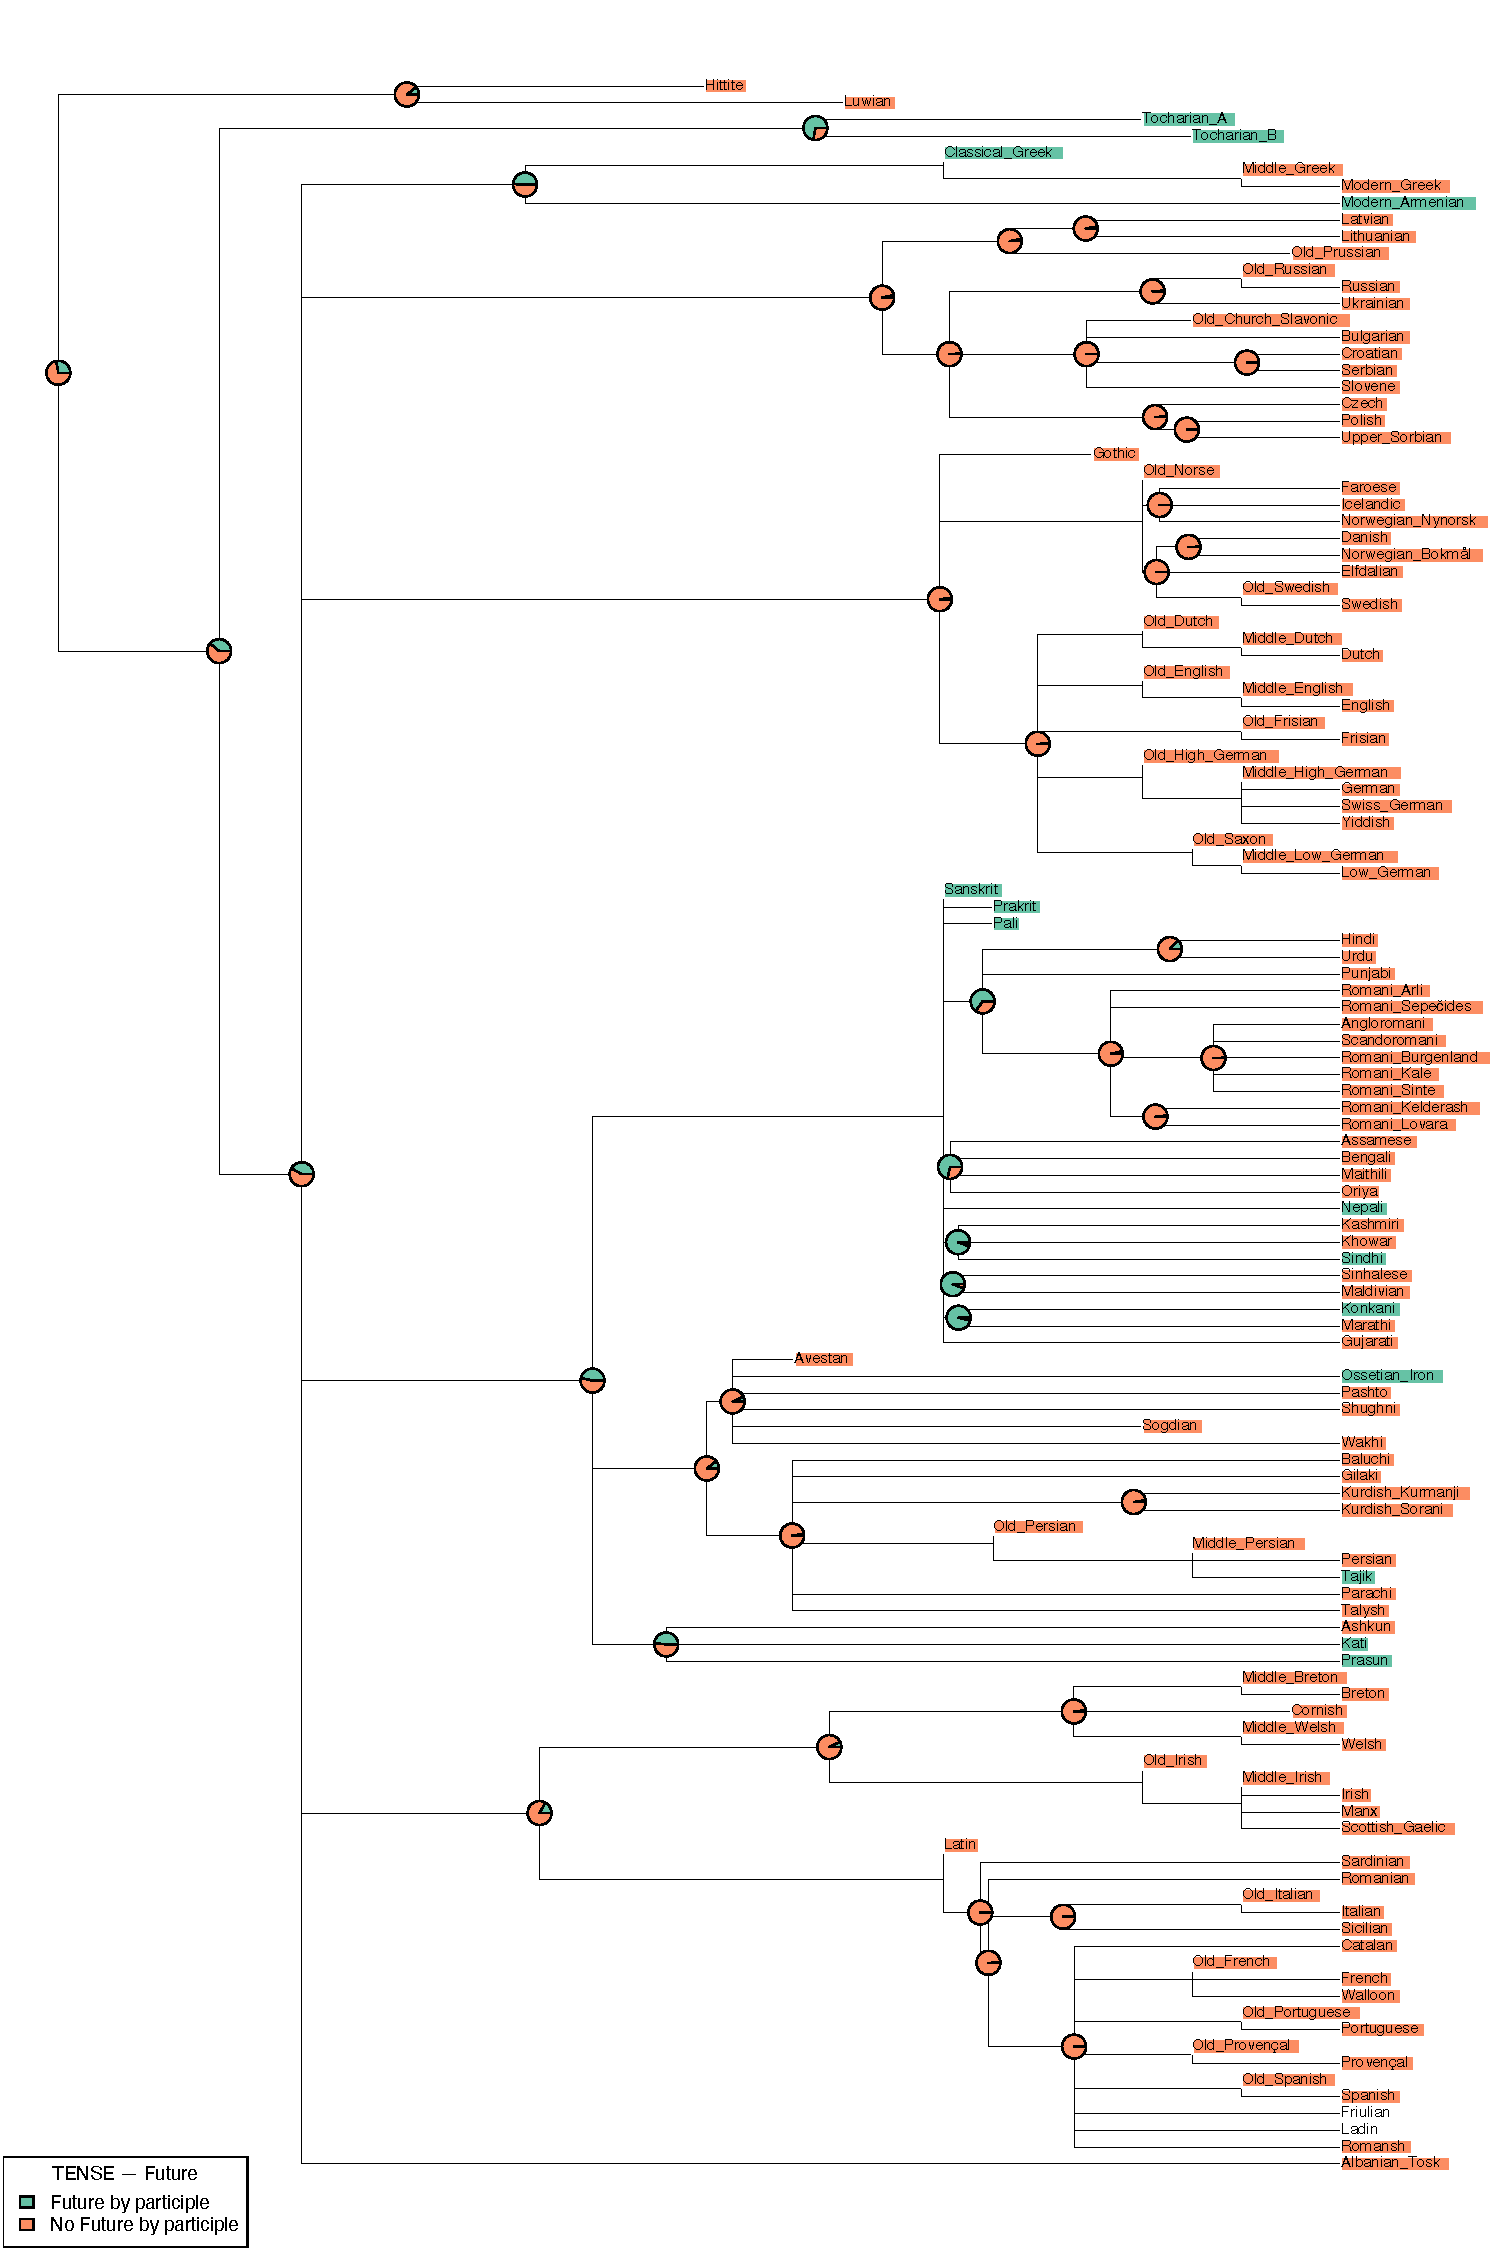
\includegraphics[width=.9\linewidth]{supp-graphics/TENSEFutureFUTParticiple.pdf}

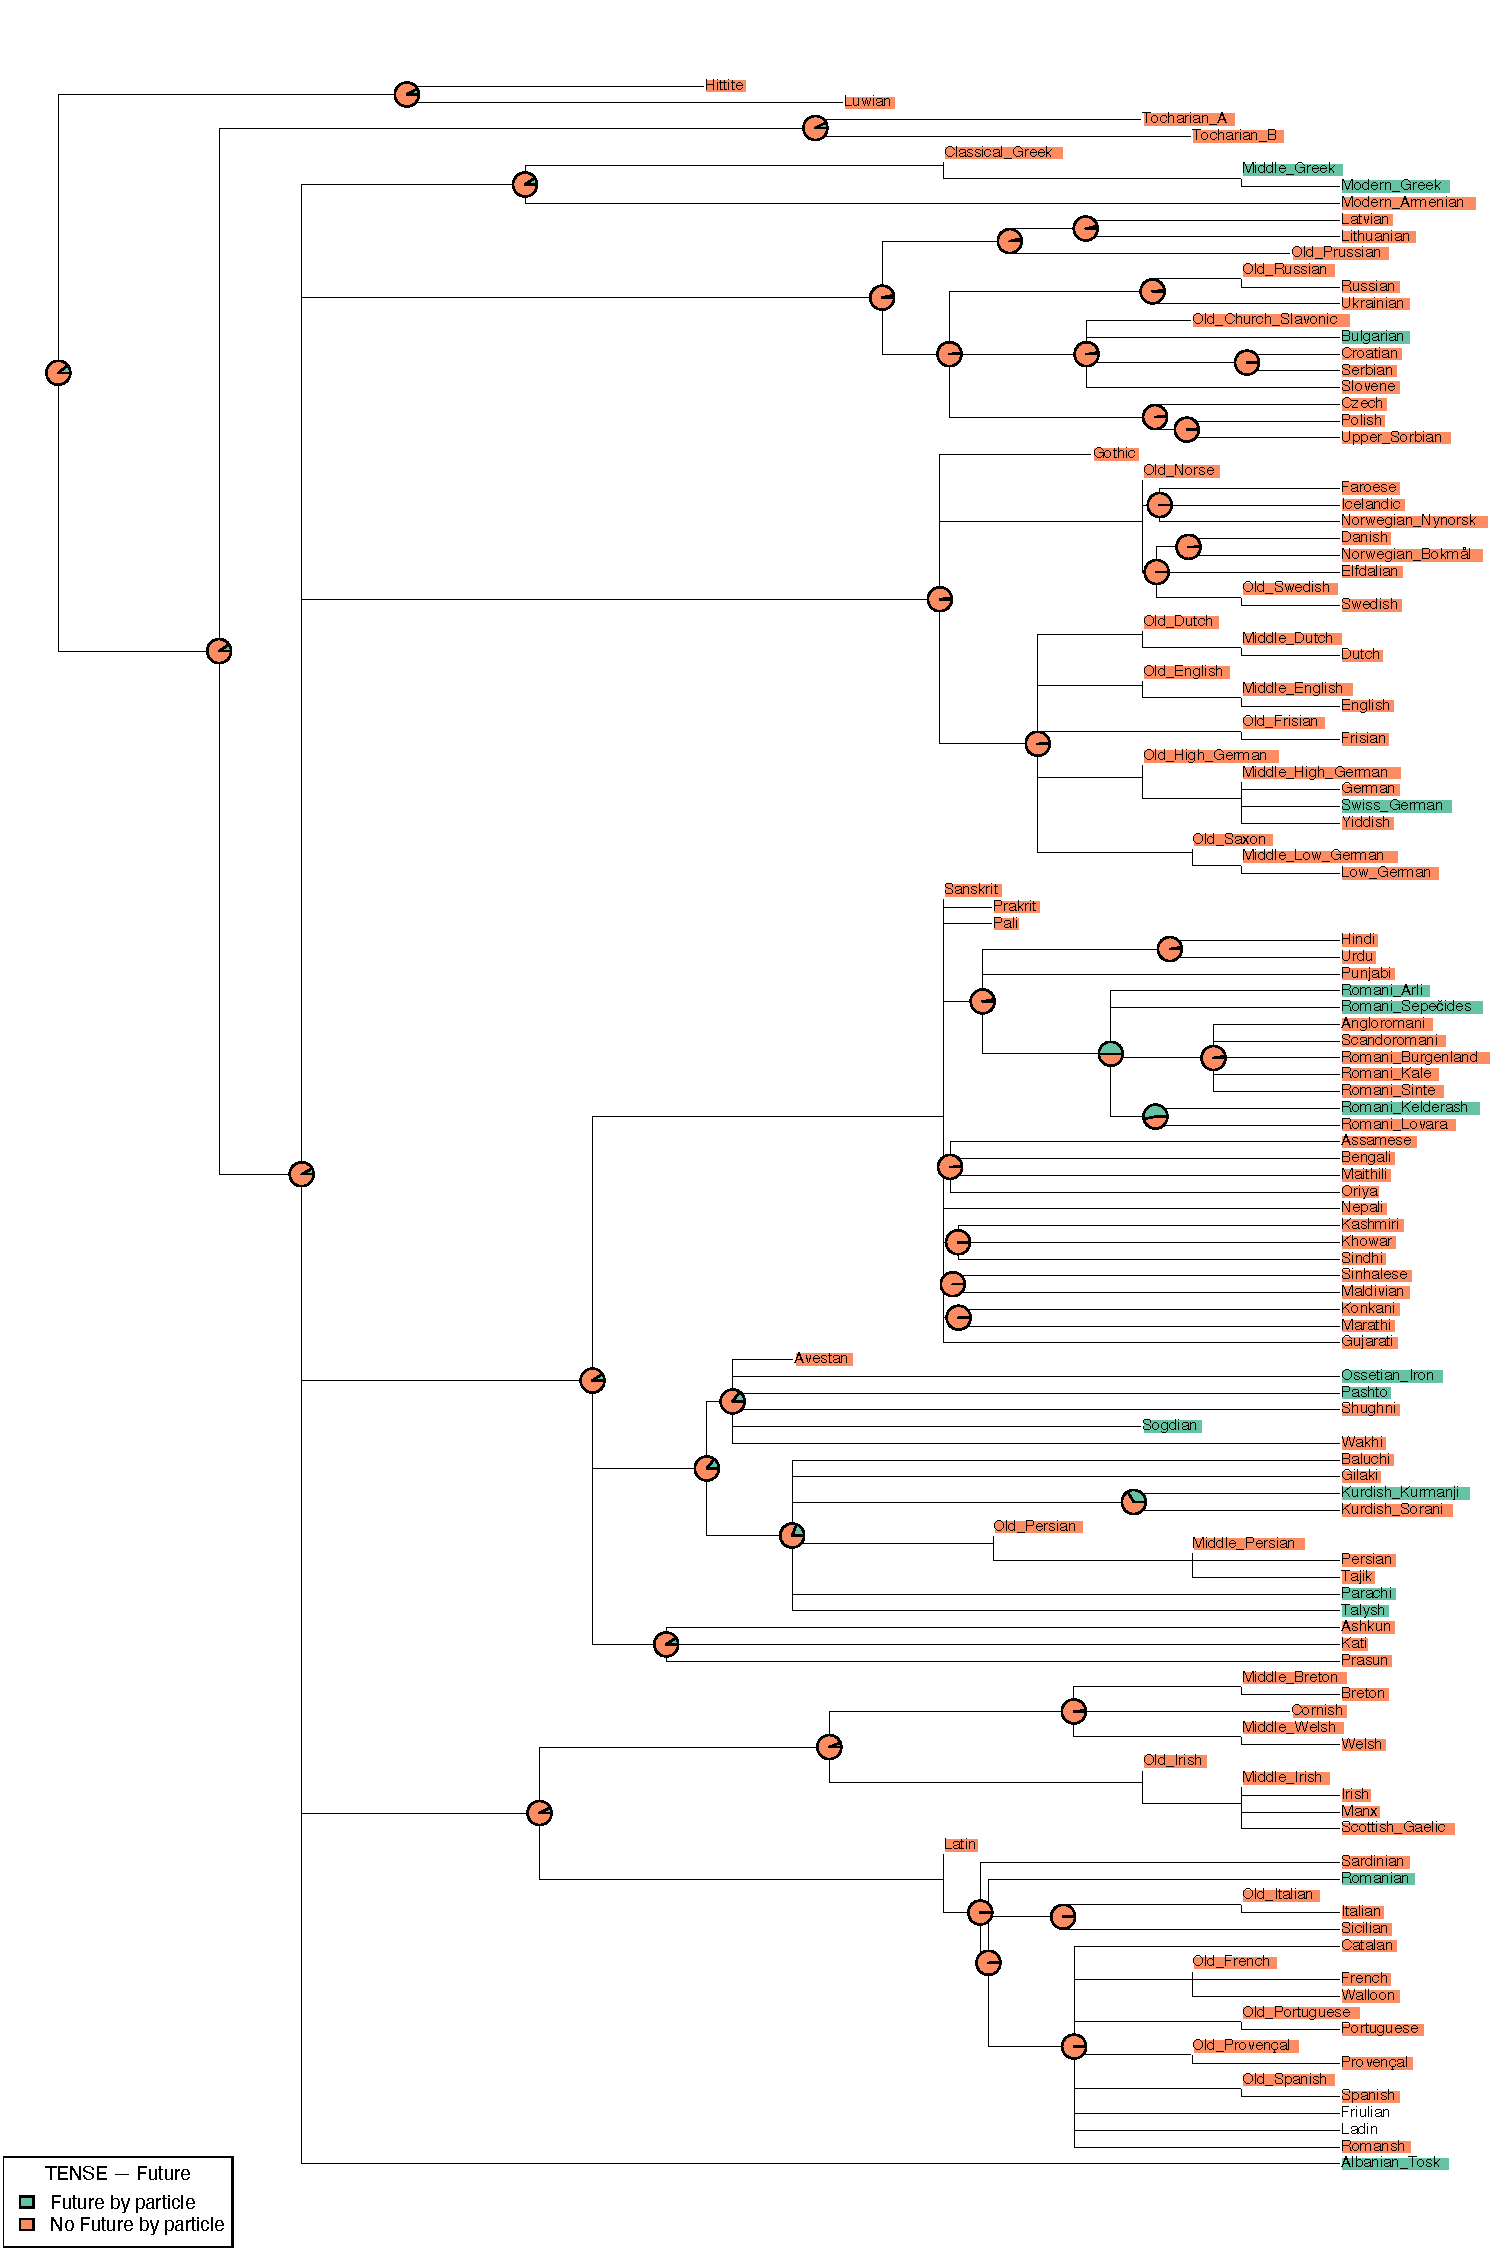
\includegraphics[width=.9\linewidth]{supp-graphics/TENSEFutureFUTParticle.pdf}

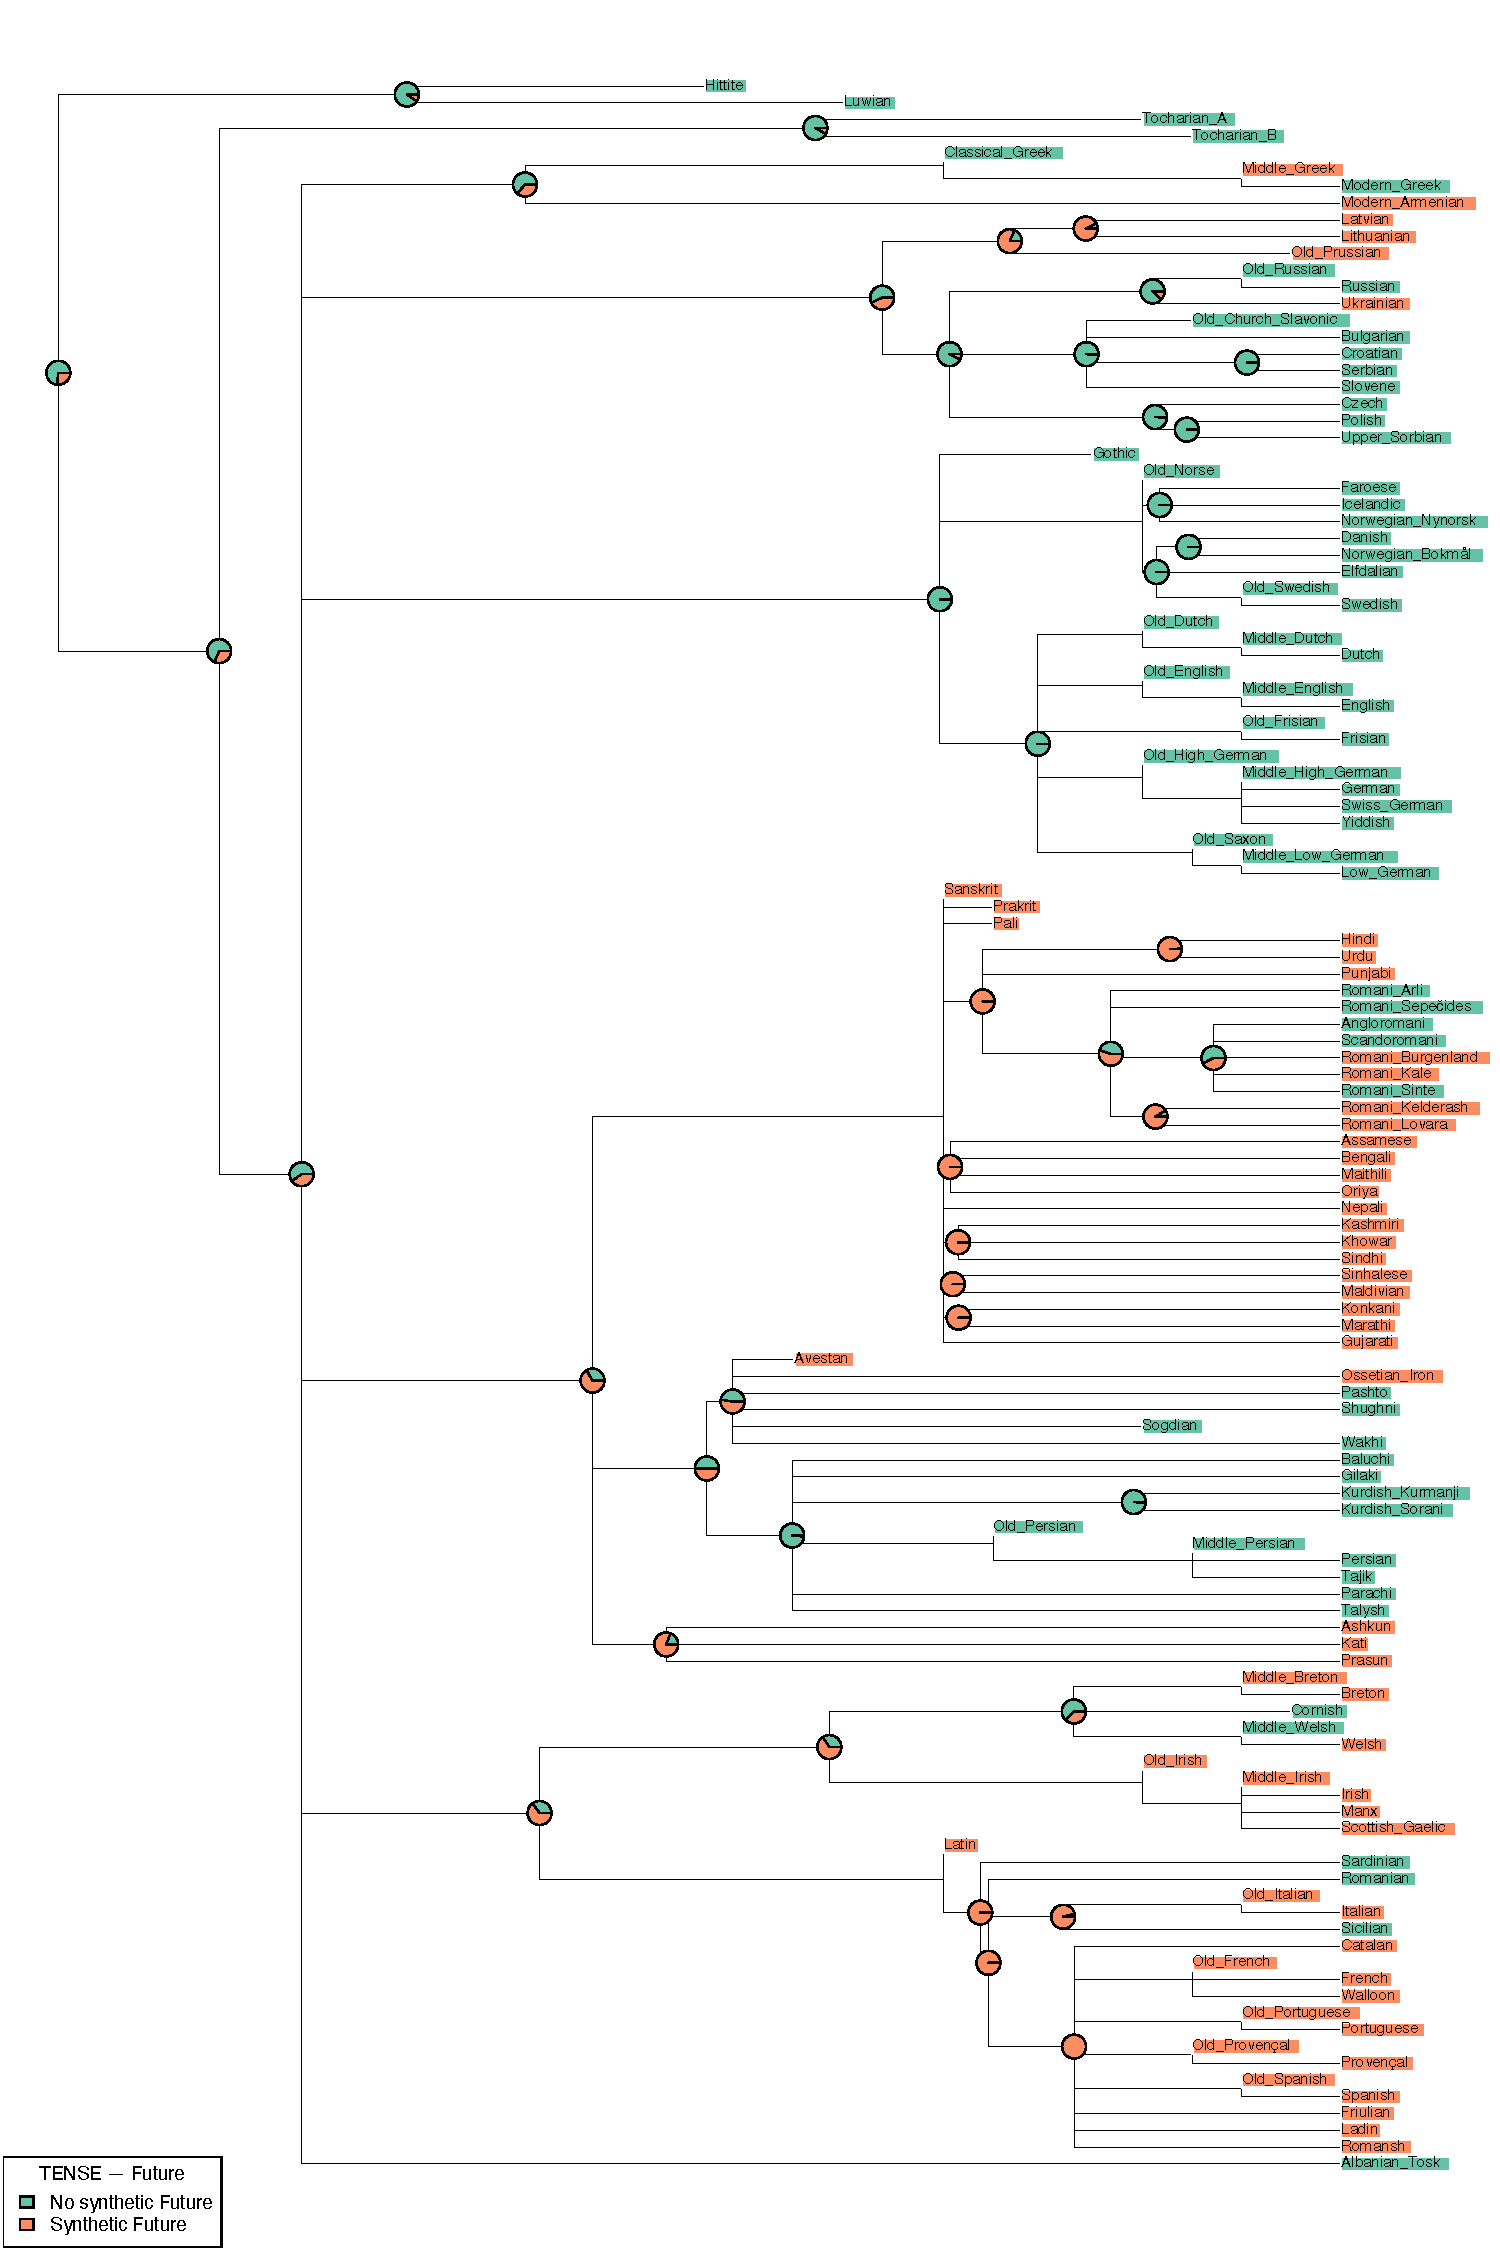
\includegraphics[width=.9\linewidth]{supp-graphics/TENSEFutureFUTSynth.pdf}

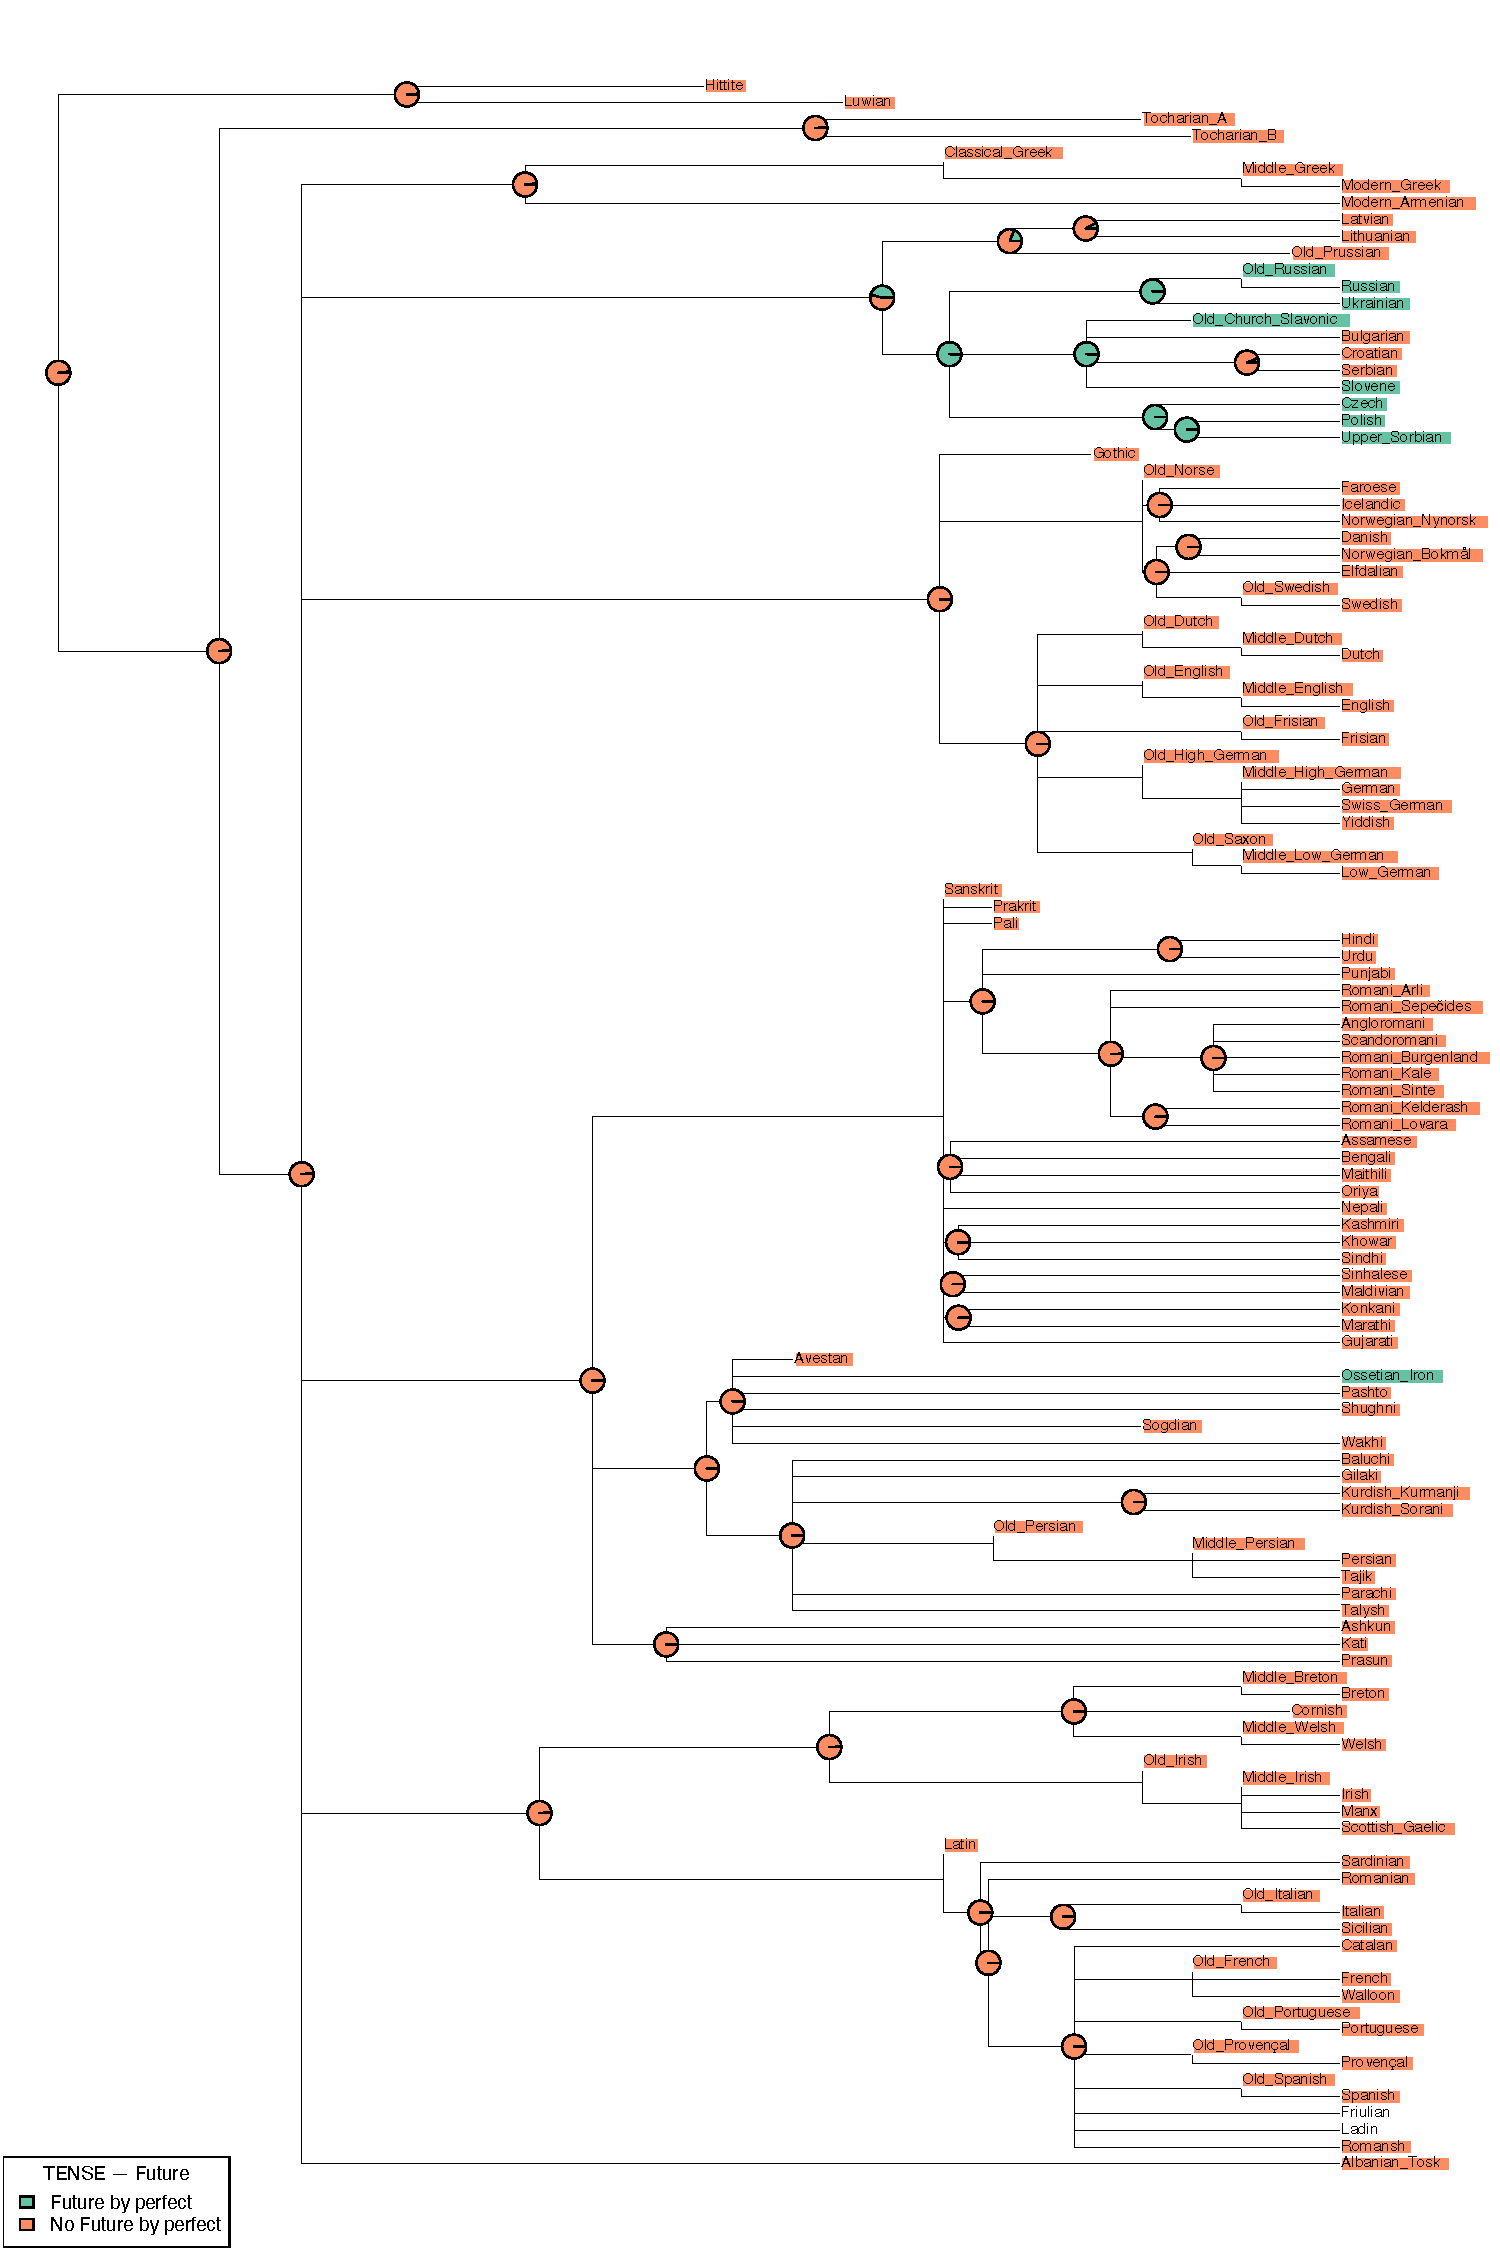
\includegraphics[width=.9\linewidth]{supp-graphics/TENSEFuturePERFFUT.pdf}

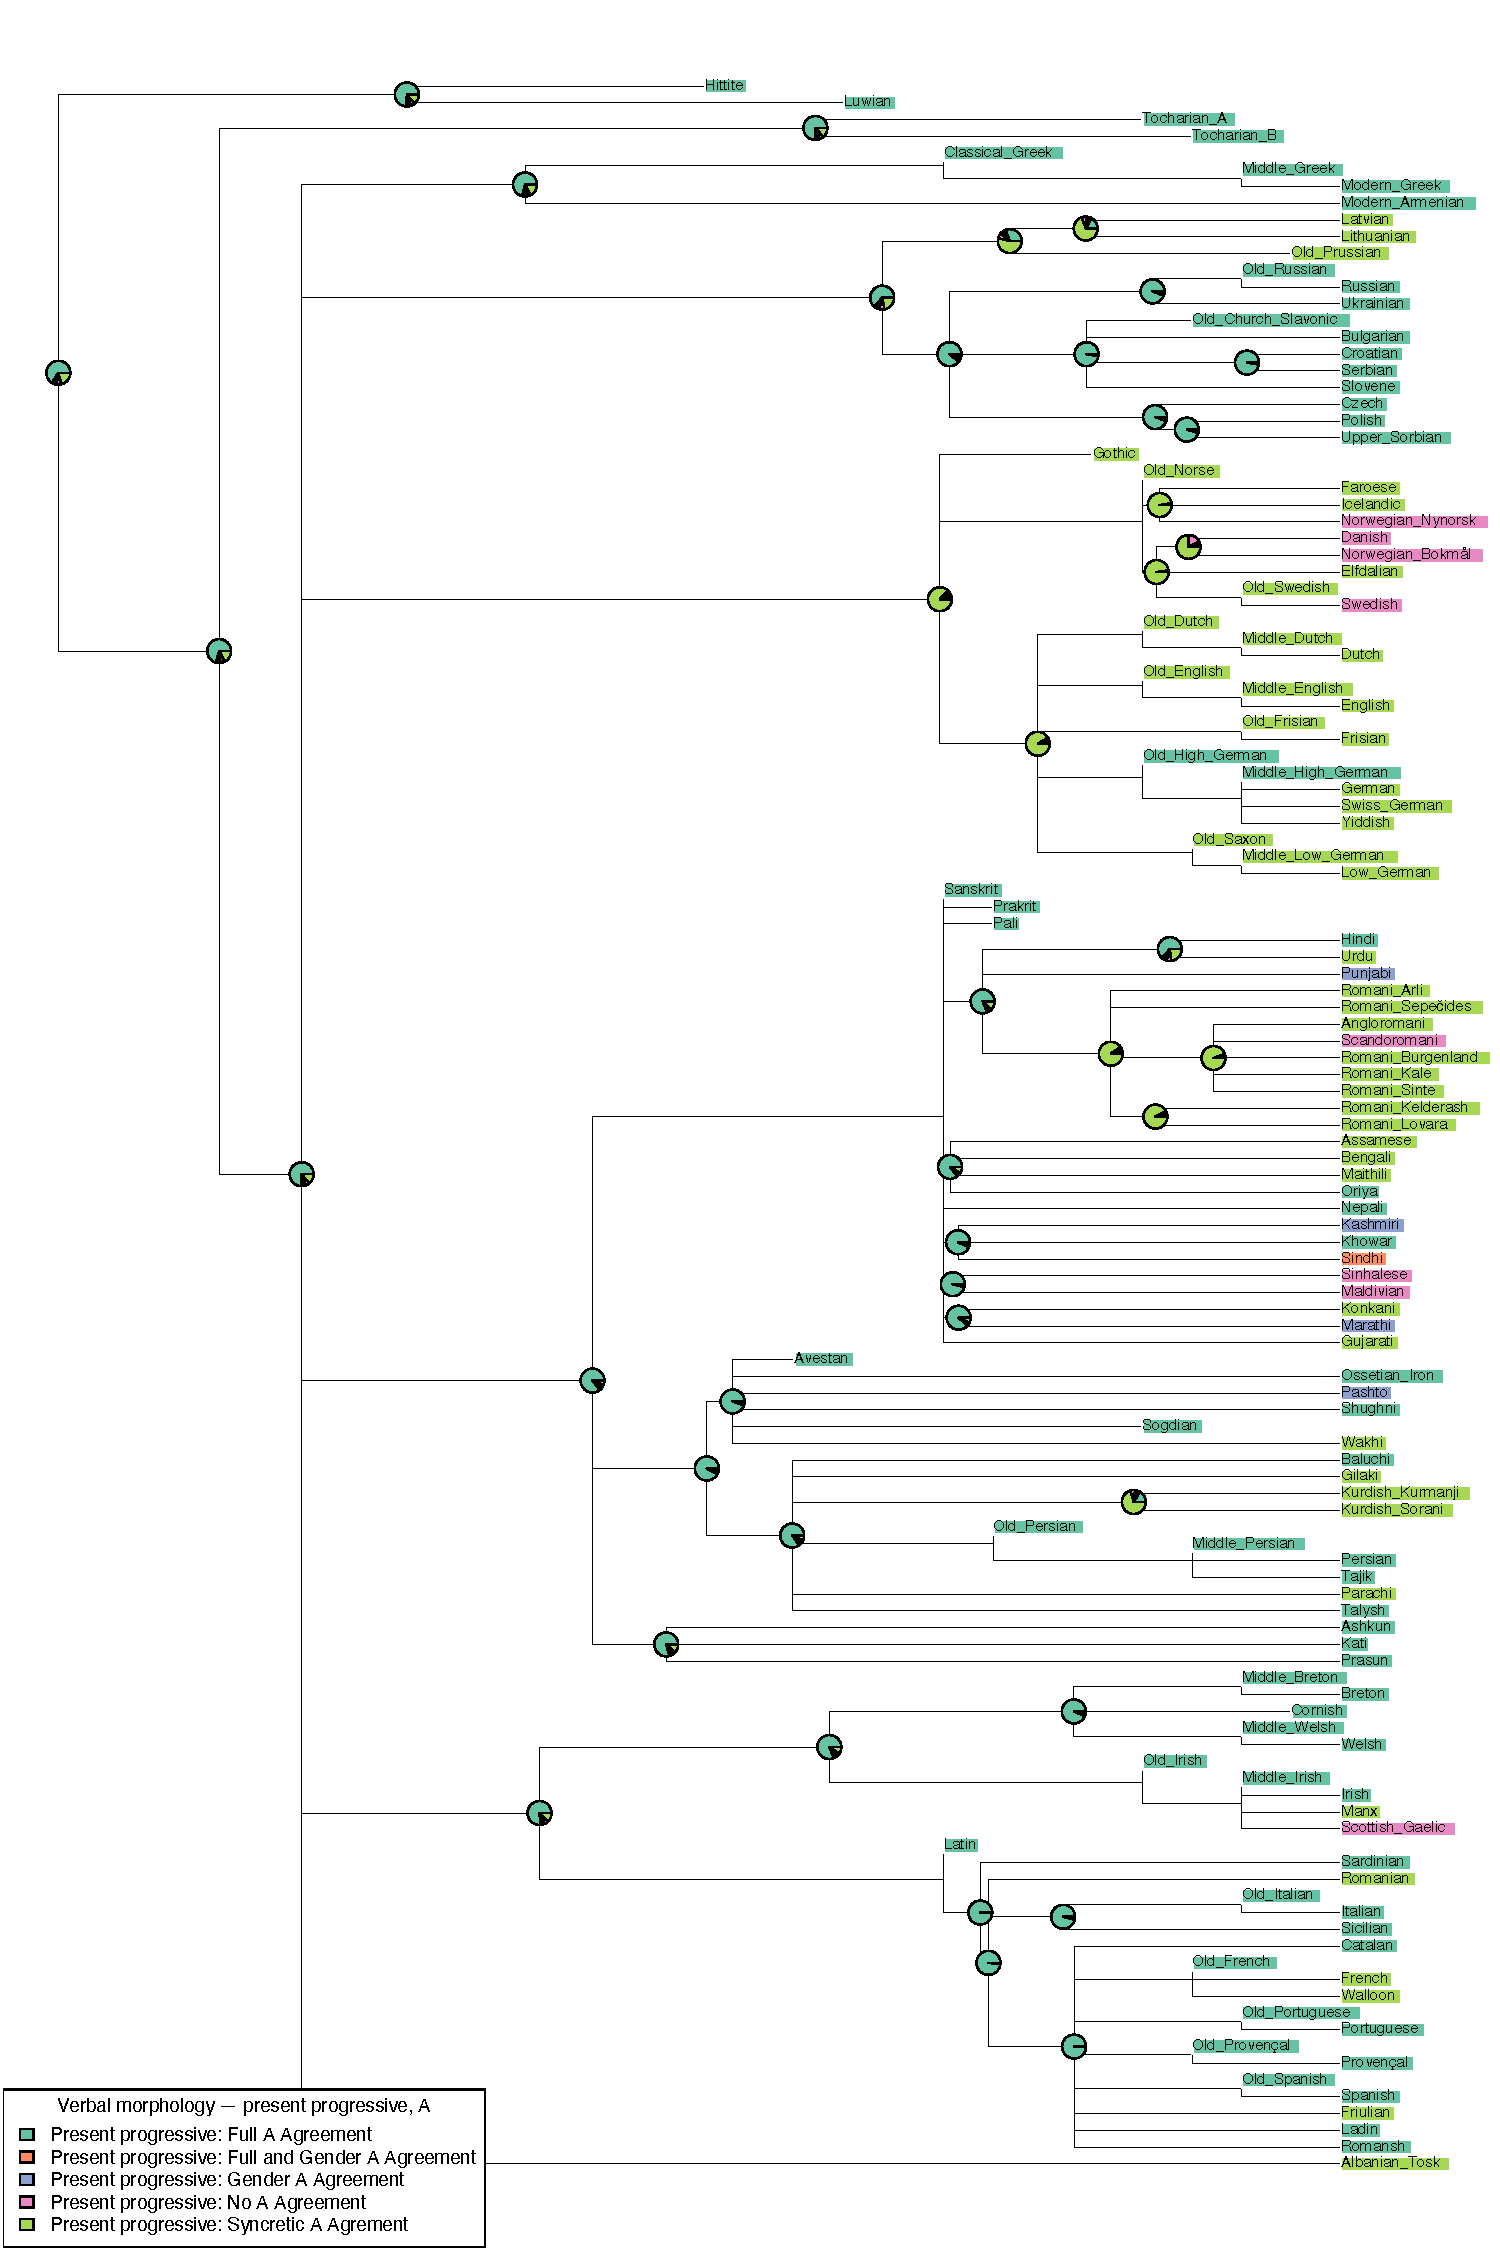
\includegraphics[width=.9\linewidth]{supp-graphics/VerbalmorphologypresentprogressiveAPROGAAGRFULLVerbalmorphologypresentprogressiveAPROGAGenderAGRVerbalmorphologypresentprogressiveAPROGNOAAGR.pdf}

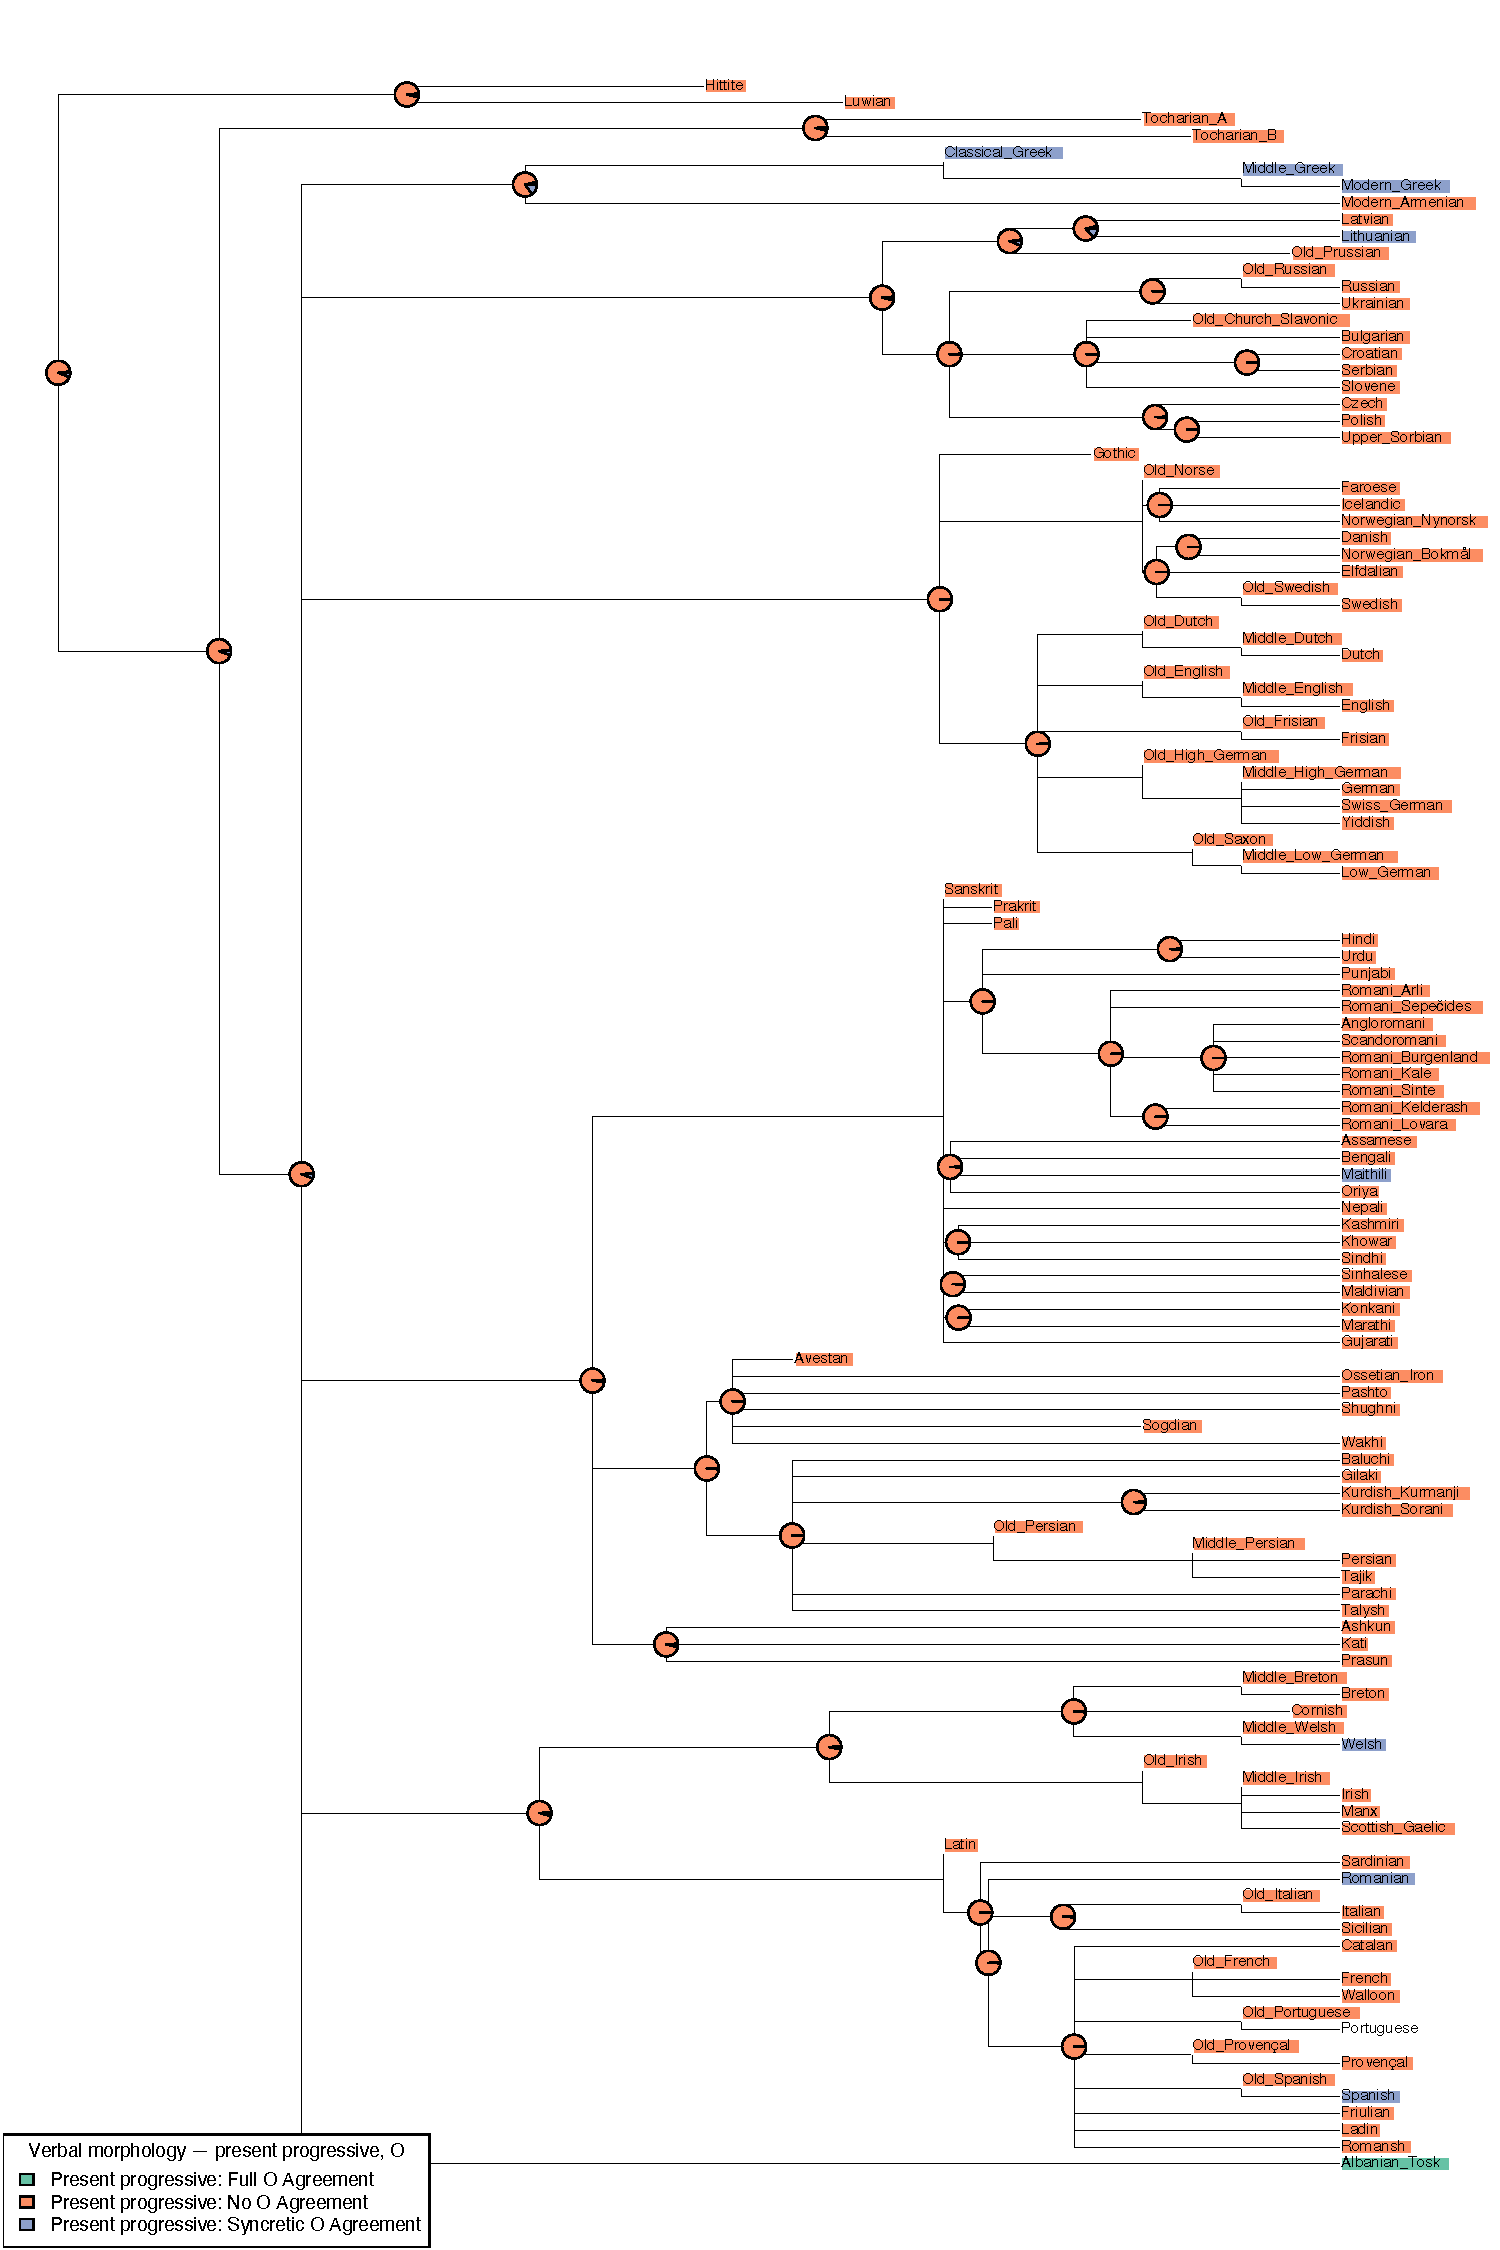
\includegraphics[width=.9\linewidth]{supp-graphics/VerbalmorphologypresentprogressiveOPROGNOOAGRVerbalmorphologypresentprogressiveOPROGOAGRFULLVerbalmorphologypresentprogressiveOPROGOGenderAGR.pdf}

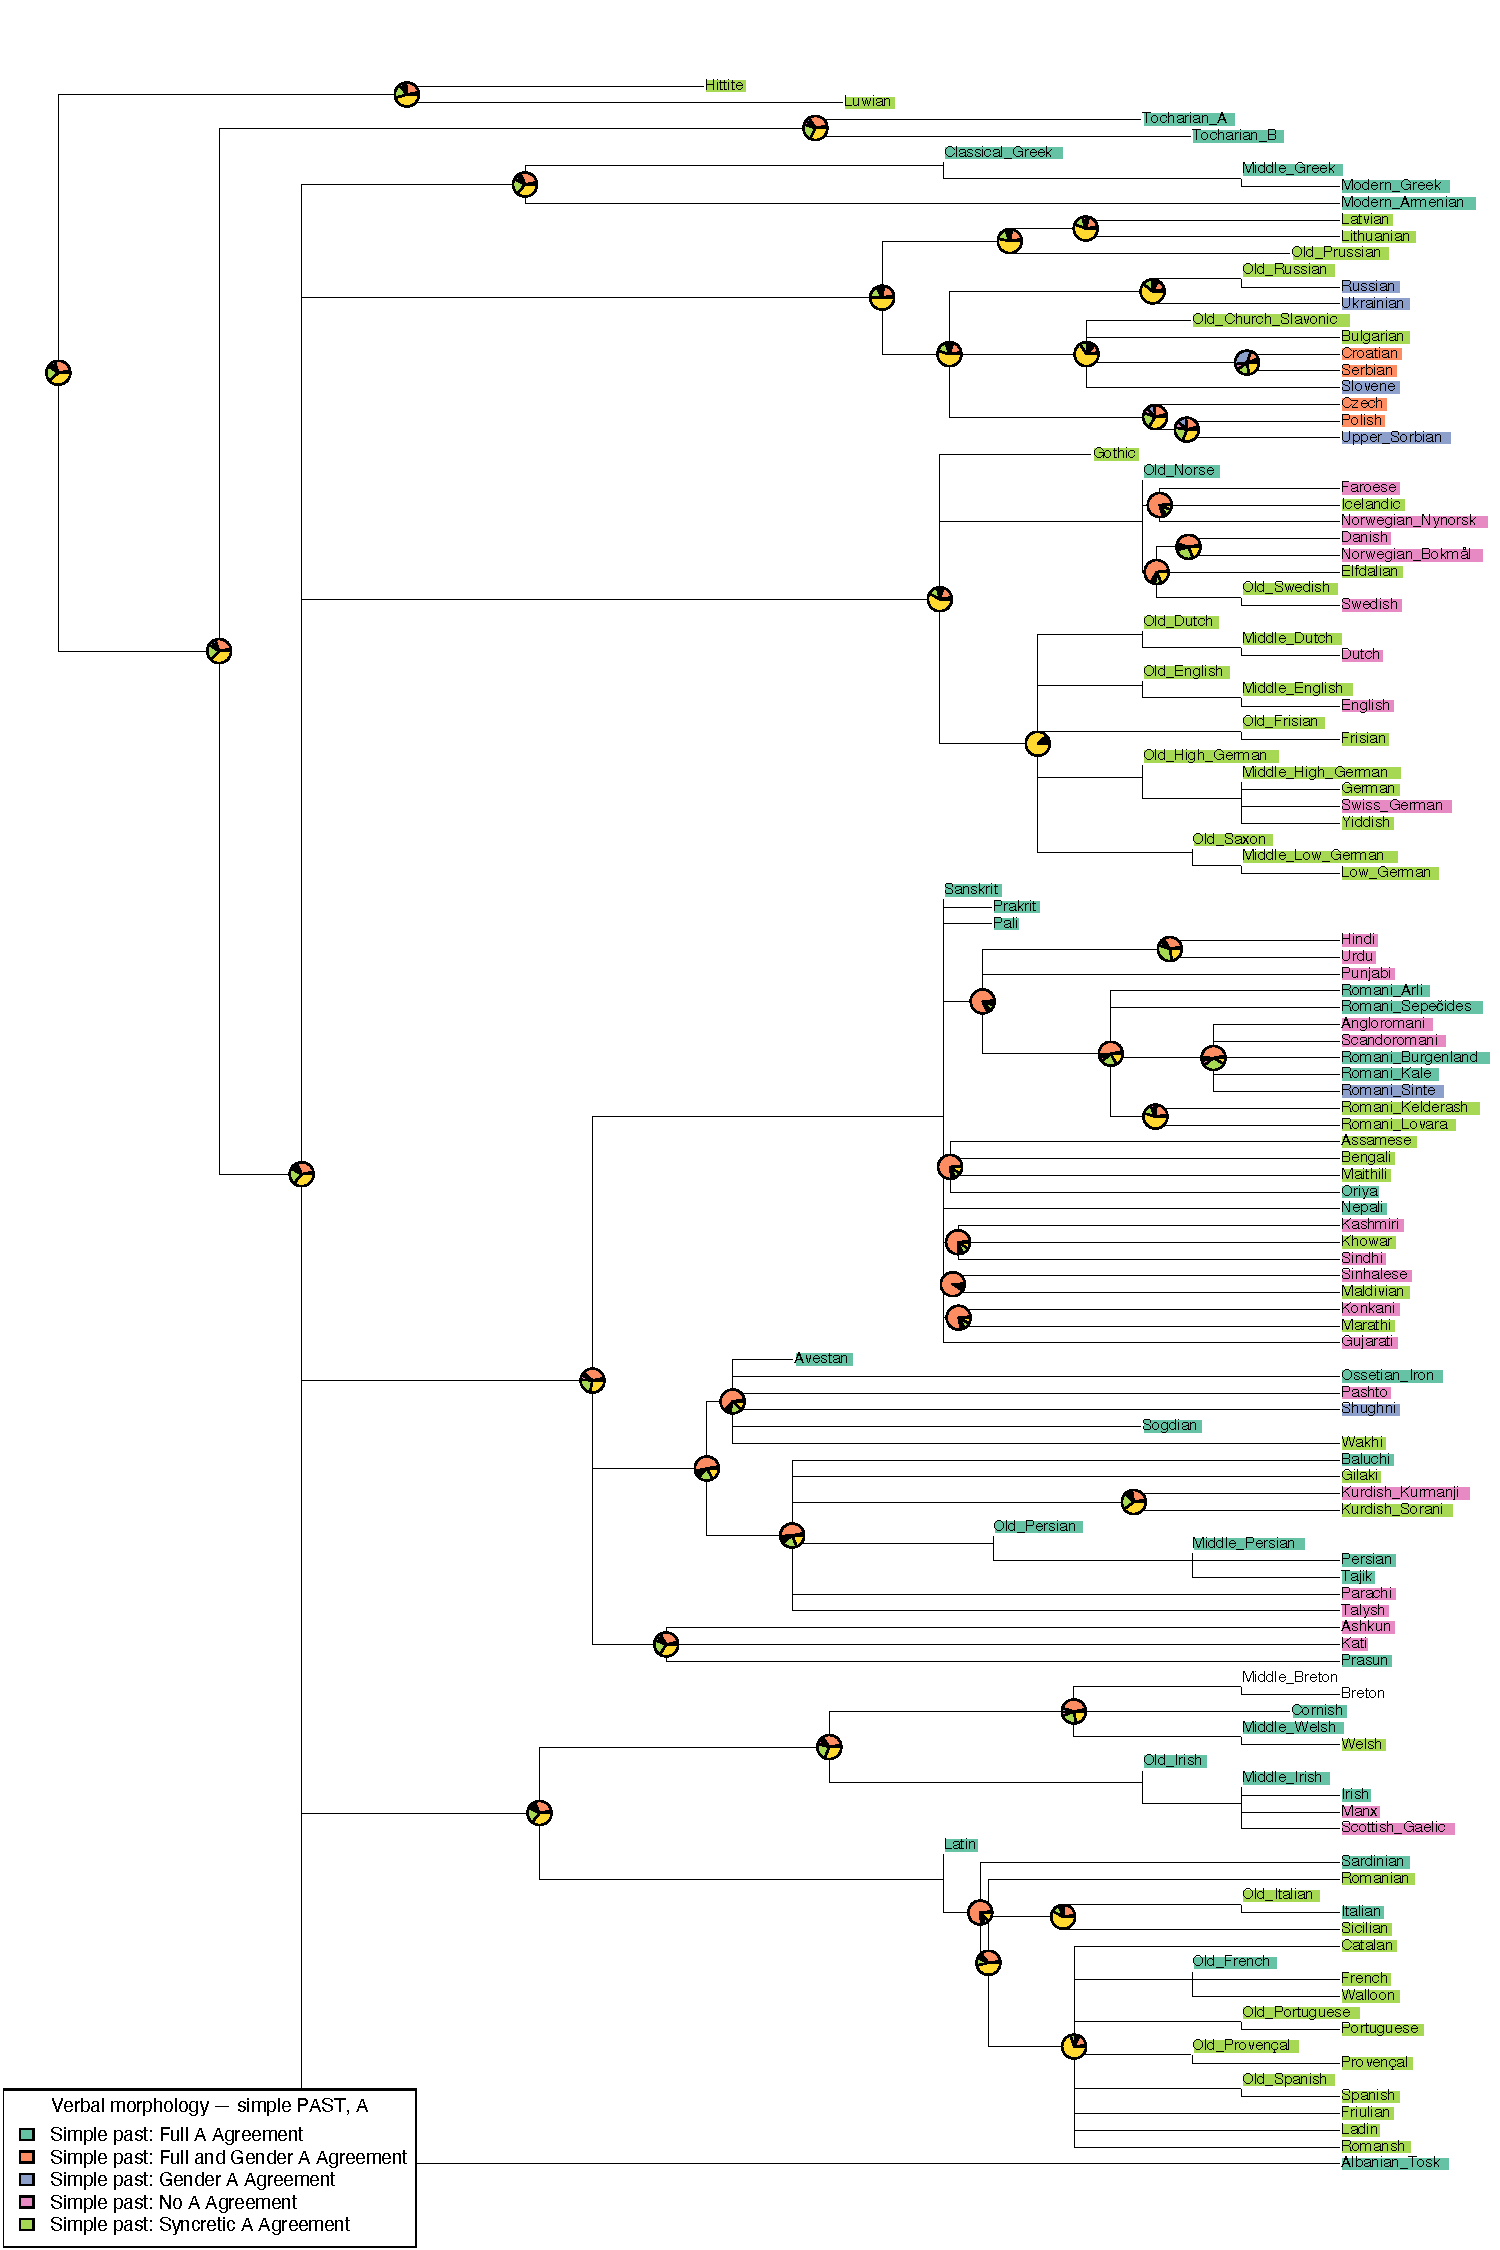
\includegraphics[width=.9\linewidth]{supp-graphics/VerbalmorphologysimplePASTAPSTAAGRFULLVerbalmorphologysimplePASTAPSTAGenderAGRVerbalmorphologysimplePASTAPSTNOAAGR.pdf}

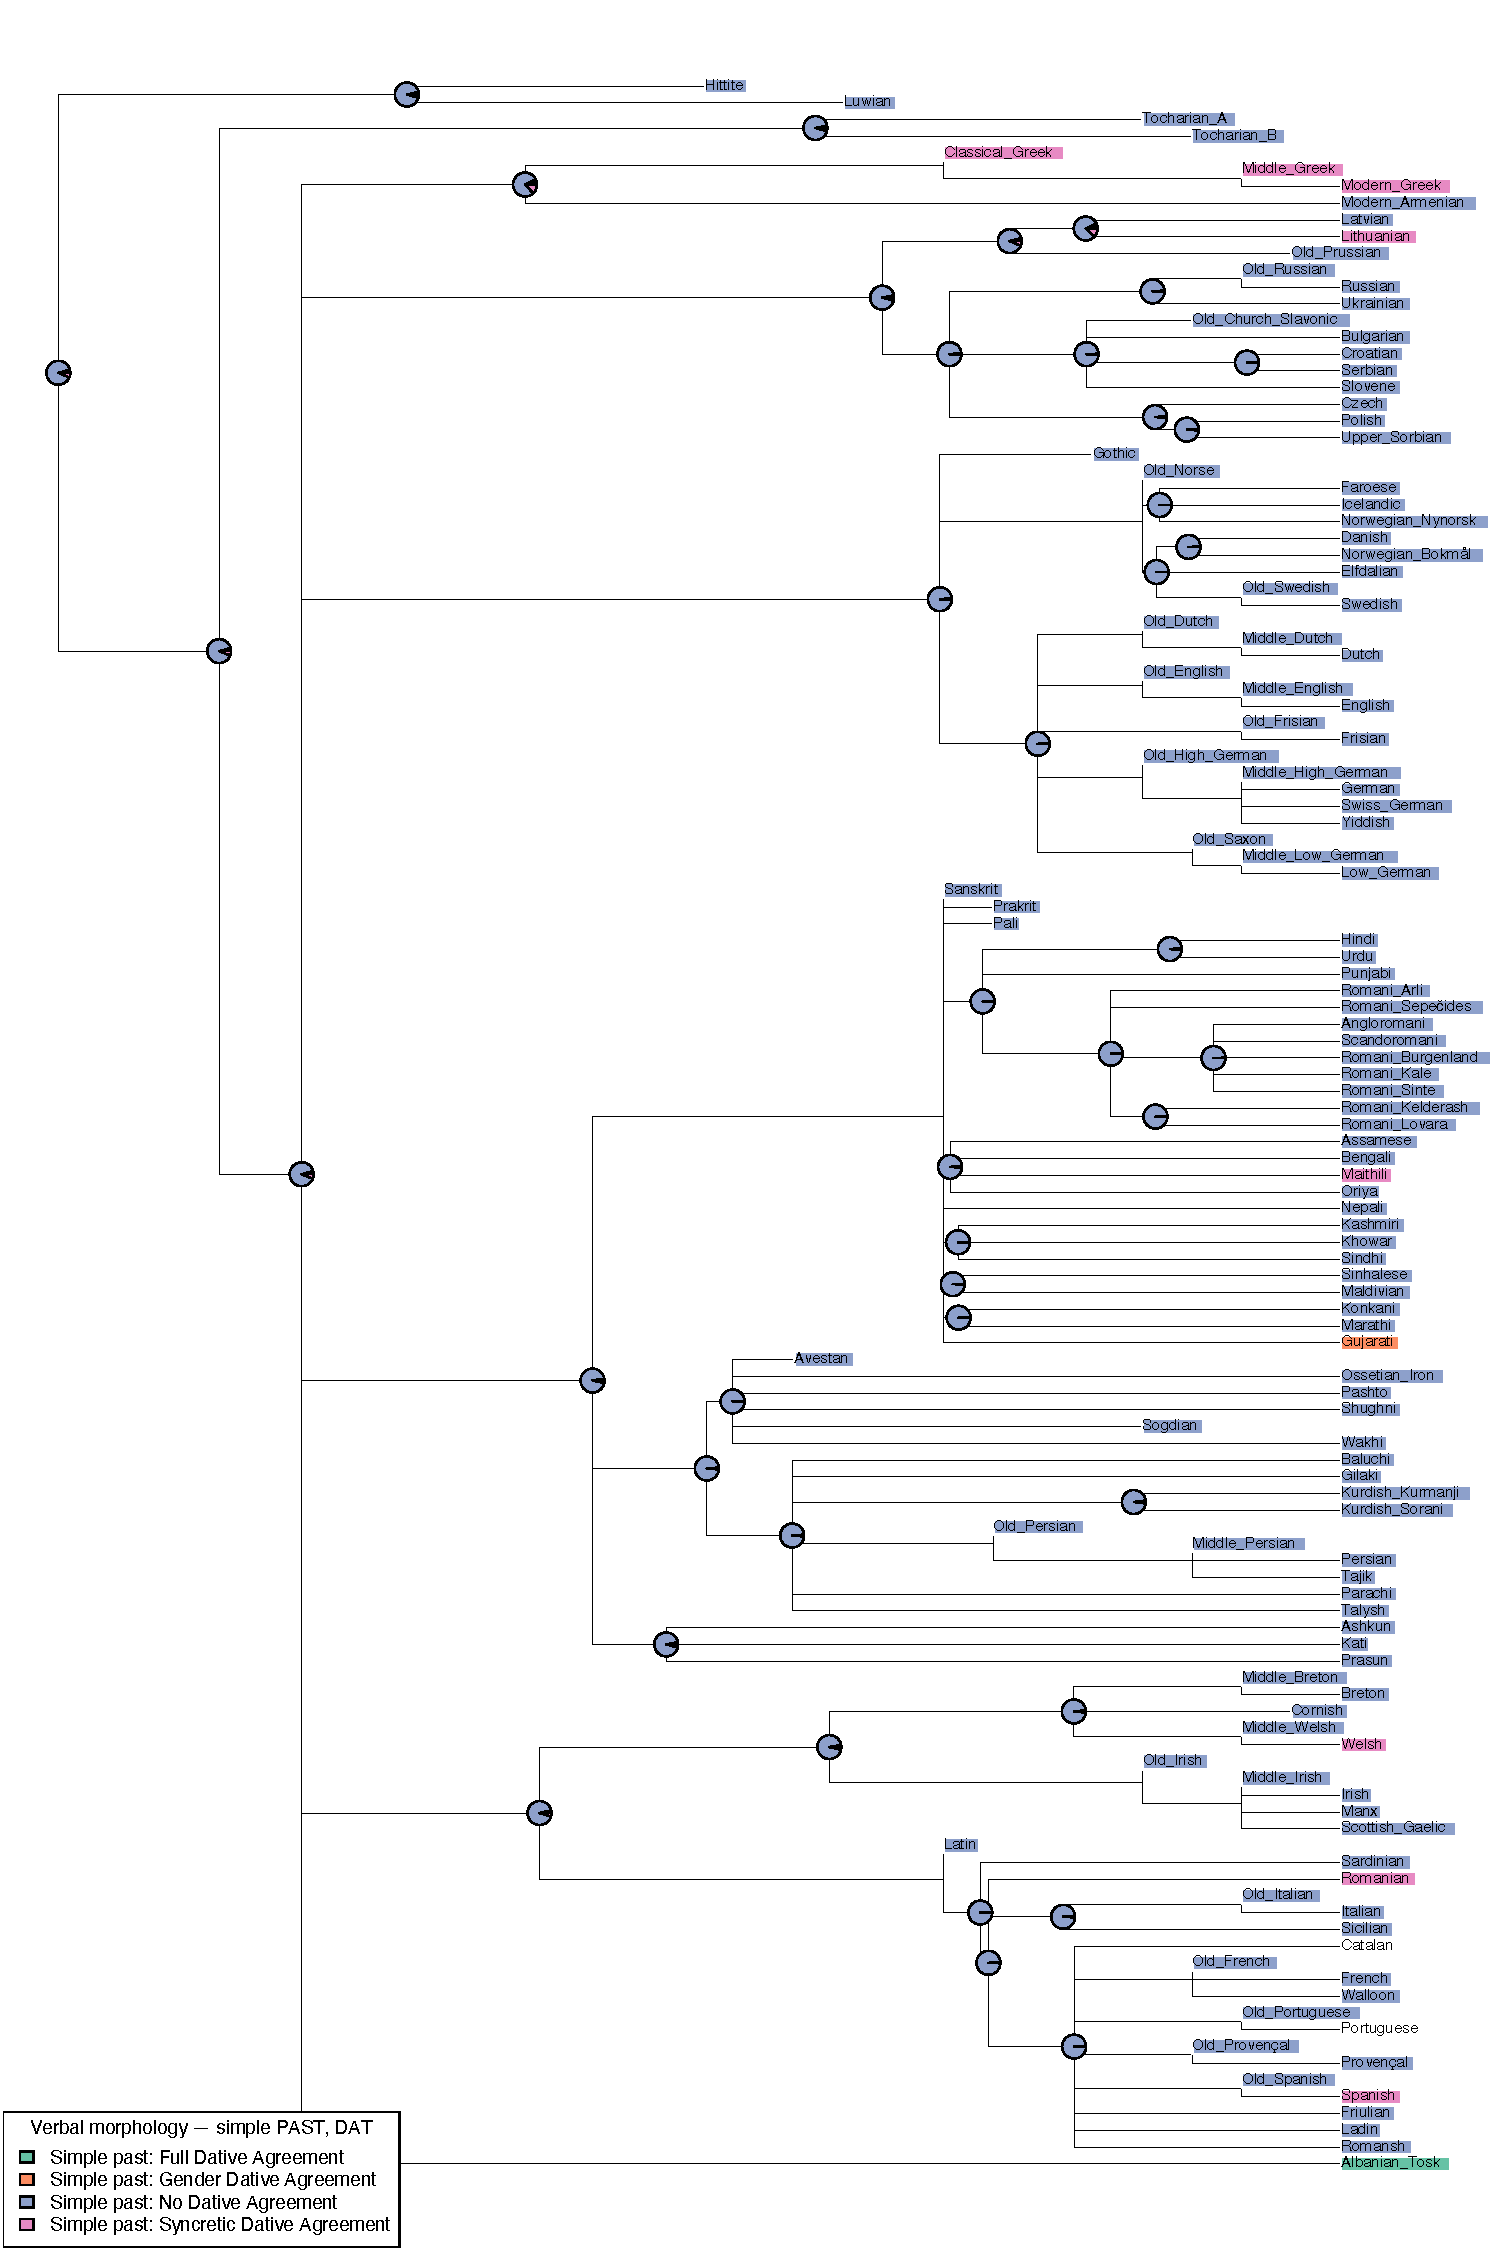
\includegraphics[width=.9\linewidth]{supp-graphics/VerbalmorphologysimplePASTDATPSTDATAGRFULLVerbalmorphologysimplePASTDATPSTDATGenderAGRVerbalmorphologysimplePASTDATPSTNODATAGR.pdf}

\includegraphics[width=.9\linewidth]{supp-graphics/VerbalmorphologysimplePASTOPSTNOOAGRVerbalmorphologysimplePASTOPSTOAGRFULLVerbalmorphologysimplePASTOPSTOGenderAGR.pdf}

\includegraphics[width=.9\linewidth]{supp-graphics/WordorderAdpositionsPost.pdf}

\includegraphics[width=.9\linewidth]{supp-graphics/WordorderAdpositionsPrep.pdf}

\includegraphics[width=.9\linewidth]{supp-graphics/WordorderCliticpronounsfiniteverb2ndpositionWordorderCliticpronounsfiniteverbOVWordorderCliticpronounsfiniteverbVO.pdf}

\includegraphics[width=.9\linewidth]{supp-graphics/WordorderCliticpronounsinfinitive2ndpositionWordorderCliticpronounsinfinitiveOVWordorderCliticpronounsinfinitiveVO.pdf}

\includegraphics[width=.9\linewidth]{supp-graphics/WordorderCliticpronounsparticiple2ndpositionWordorderCliticpronounsparticipleOVWordorderCliticpronounsparticipleVO.pdf}

\includegraphics[width=.9\linewidth]{supp-graphics/WordorderInfinitiveOVWordorderInfinitiveVO.pdf}

\includegraphics[width=.9\linewidth]{supp-graphics/WordorderMainclausesSOVWordorderMainclausesSVOWordorderMainclausesV2WordorderMainclausesVSO.pdf}

\includegraphics[width=.9\linewidth]{supp-graphics/WordorderNounadjectiveANWordorderNounadjectiveNA.pdf}

\includegraphics[width=.9\linewidth]{supp-graphics/WordorderParticipleOVWordorderParticipleVO.pdf}

\includegraphics[width=.9\linewidth]{supp-graphics/WordorderSubordinateclauseSOVWordorderSubordinateclauseSVOWordorderSubordinateclauseV2WordorderSubordinateclauseVSO.pdf}

\includegraphics[width=.9\linewidth]{supp-graphics/WordorderWHelementWHV.pdf}

\includegraphics[width=.9\linewidth]{supp-graphics/WordorderWHelementWHinitial.pdf}

\subsection*{S9}

Tree sample of Indo-European languages used for this paper's experiments.

\includegraphics[width=.6\linewidth]{tree-sample.pdf}

\end{document}
